\documentclass[a4paper, 10pt, fleqn, twosided]{memoir}

\usepackage{pgf}
\usepackage[paper = a4paper, left = 25mm, width = 160mm, top = 25mm, bottom = 25mm]{geometry}
\usepackage{apacite}
\usepackage{setspace}
\usepackage{graphicx}
\usepackage[export]{adjustbox}
\usepackage{amsmath}
\usepackage{graphics}
\usepackage{multicol}
\usepackage{multirow}
\usepackage{wasysym}
\usepackage{booktabs}
\usepackage[utf8]{inputenc}
\usepackage{todonotes}
\usepackage{tikz}
\usepackage{tcolorbox}
\usepackage{epigraph}
\usepackage{xcolor}
\usepackage{pdflscape}
\setlength{\parindent}{0em}
\setlength{\parskip}{14pt}


\usepackage[light]{iwona}
\usepackage[T1]{fontenc}
\usepackage{tabularx}
\newcolumntype{Y}{>{\raggedright\arraybackslash}X}

\counterwithout{section}{chapter}
\setsecnumdepth{subsubsection}
\setcounter{tocdepth}{3}

\usepackage{listings}% http://ctan.org/pkg/listings
\lstset{
  basicstyle=\ttfamily,
  mathescape
}

\definecolor{code}{cmyk}{1,.60,0,.40}
\definecolor{outpt}{RGB}{40, 205, 175}
\definecolor{funct}{RGB}{151, 67, 145}
\definecolor{interp}{RGB}{255, 191, 0}

\DeclareFixedFont{\titlefont}{T1}{ppl}{b}{it}{0.5in}

\raggedbottom

\makeatletter
\def\printauthor{%
    {\large \@author}}
\makeatother
\author{%
    Sharon Nielsen \\
    Biometrician \\
    \texttt{sharon.nielsen@adelaide.edu.au} \vspace{20mm}
     }

% The following code is borrowed from: https://tex.stackexchange.com/a/86310/10898

\newcommand\titlepagedecoration{%
\begin{tikzpicture}[remember picture,overlay,shorten >= -10pt]

\coordinate (aux1) at ([yshift=-15pt]current page.north east);
\coordinate (aux2) at ([yshift=-410pt]current page.north east);
\coordinate (aux3) at ([xshift=-4.5cm]current page.north east);
\coordinate (aux4) at ([yshift=-150pt]current page.north east);

\begin{scope}[code!40,line width=12pt,rounded corners=12pt]
\draw
  (aux1) -- coordinate (a)
  ++(225:5) --
  ++(-45:5.1) coordinate (b);
\draw[shorten <= -10pt]
  (aux3) --
  (a) --
  (aux1);
\draw[opacity=0.6,code,shorten <= -10pt]
  (b) --
  ++(225:2.2) --
  ++(-45:2.2);
\end{scope}
\draw[code,line width=8pt,rounded corners=8pt,shorten <= -10pt]
  (aux4) --
  ++(225:0.8) --
  ++(-45:0.8);
\begin{scope}[code!70,line width=6pt,rounded corners=8pt]
\draw[shorten <= -10pt]
  (aux2) --
  ++(225:3) coordinate[pos=0.45] (c) --
  ++(-45:3.1);
\draw
  (aux2) --
  (c) --
  ++(135:2.5) --
  ++(45:2.5) --
  ++(-45:2.5) coordinate[pos=0.3] (d);
\draw
  (d) -- +(45:1);
\end{scope}
\end{tikzpicture}%
}

\tcbuselibrary{skins}

\newtcolorbox{application}[2][]{%
    % [#1]: Extra options for the tcolorbox
    % {#2}: Title of box
    title= {#2},
    enhanced,
    skin=enhancedlast,
    sharp corners,
    colframe = black,
    colback = white,
    drop fuzzy shadow,
    boxrule = 0.41pt, %Width of line
    borderline north={1.1mm}{-1.1mm}{black}, %The two distances must be equal magnitude but opposite in sign
    attach boxed title to top left={
        xshift = -2mm,
        yshift=-0.5mm,
        yshifttext=-1mm
    },
    coltitle = black!50!blue,
    fonttitle = \Large\itshape,
    boxed title style = {
        colframe = white,
        colback = white,
        sharp corners
    },#1
}


\begin{document}

\raggedbottom
\begin{titlingpage}

\noindent
\titlefont Statistical Analysis of \newline Agronomic Experiments\par
\null\vfill
\vspace*{1cm}
\noindent
\hfill
\begin{minipage}{0.35\linewidth}
    \begin{flushright}
        \printauthor
    \end{flushright}

\end{minipage}
%
%%% logos go here ...

\begin{tabular}{rr}
	
\includegraphics[height = 1cm, keepaspectratio]{SARDI}
	
\includegraphics[height = 1cm, keepaspectratio]{SAGI}
	
\includegraphics[height = 1cm, keepaspectratio]{UoAsmall}
	
\includegraphics[height = 1cm, keepaspectratio]{BiometryHub}
	
\includegraphics[height = 1cm, keepaspectratio]{GRDC}
\end{tabular}\\[10mm]


\titlepagedecoration
\end{titlingpage}
\clearpage

\tableofcontents
\clearpage
\chapter{Statistical Analysis of Agronomic Experiments}

This course is based heavily on information in Statistical Methods in Biology: Design and Analysis of Experiments and Regression
\cite{welham2014statistical}, so rather than referencing this book throughout the workbook I acknowledge it here.


\begin{figure}[!hbtp]
\centering
\fbox{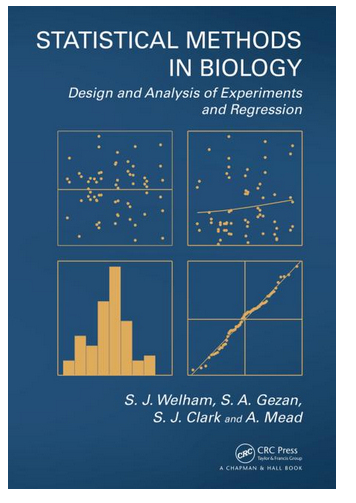
\includegraphics[width=0.5\textwidth]{welham}}
\caption{Statistical Methods in Biology: Design and Analysis of Experiments and Regression}
\label{fig:welham}
\end{figure}

\clearpage
\section{Data Analysis - A Cyclical Process}
Data analysis is an important part of the scientific process and can be done by following a process but it is really
crucial you examine all the results in the context of the analysis. As a result the data analysis process is not a
linear process but a cyclical one. We will discuss this through the workshop but first we will explore the different
types of analysis covered in this workshop.

\section{Types of Analyses}

The type of analysis required depends on:

\begin{enumerate}
\item the aim of the analysis (exploring relationships or the effect of a treatment or some other aim)
\item the type of data of the response variable (quantitative or qualitative)
\item the type of data of the explanatory variable/s (quantitative and/or qualitative)
\item the design of the experiment
\item whether the model assumptions are met
\end{enumerate}

The flow diagram (Figure \ref{fig:lmflow}) helps decide what model is appropriate for the different data types and the
number of explanatory variables.

\clearpage
\begin{landscape}
\begin{figure}[!hbtp]
\centering
\fbox{\includegraphics[width = 20cm]{LMFlowChart}}
\caption{Decision diagram for data analysis}
\label{fig:lmflow}
\end{figure}
\end{landscape}


\section{Data Types}

\begin{figure}[!hbtp]
\centering
\fbox{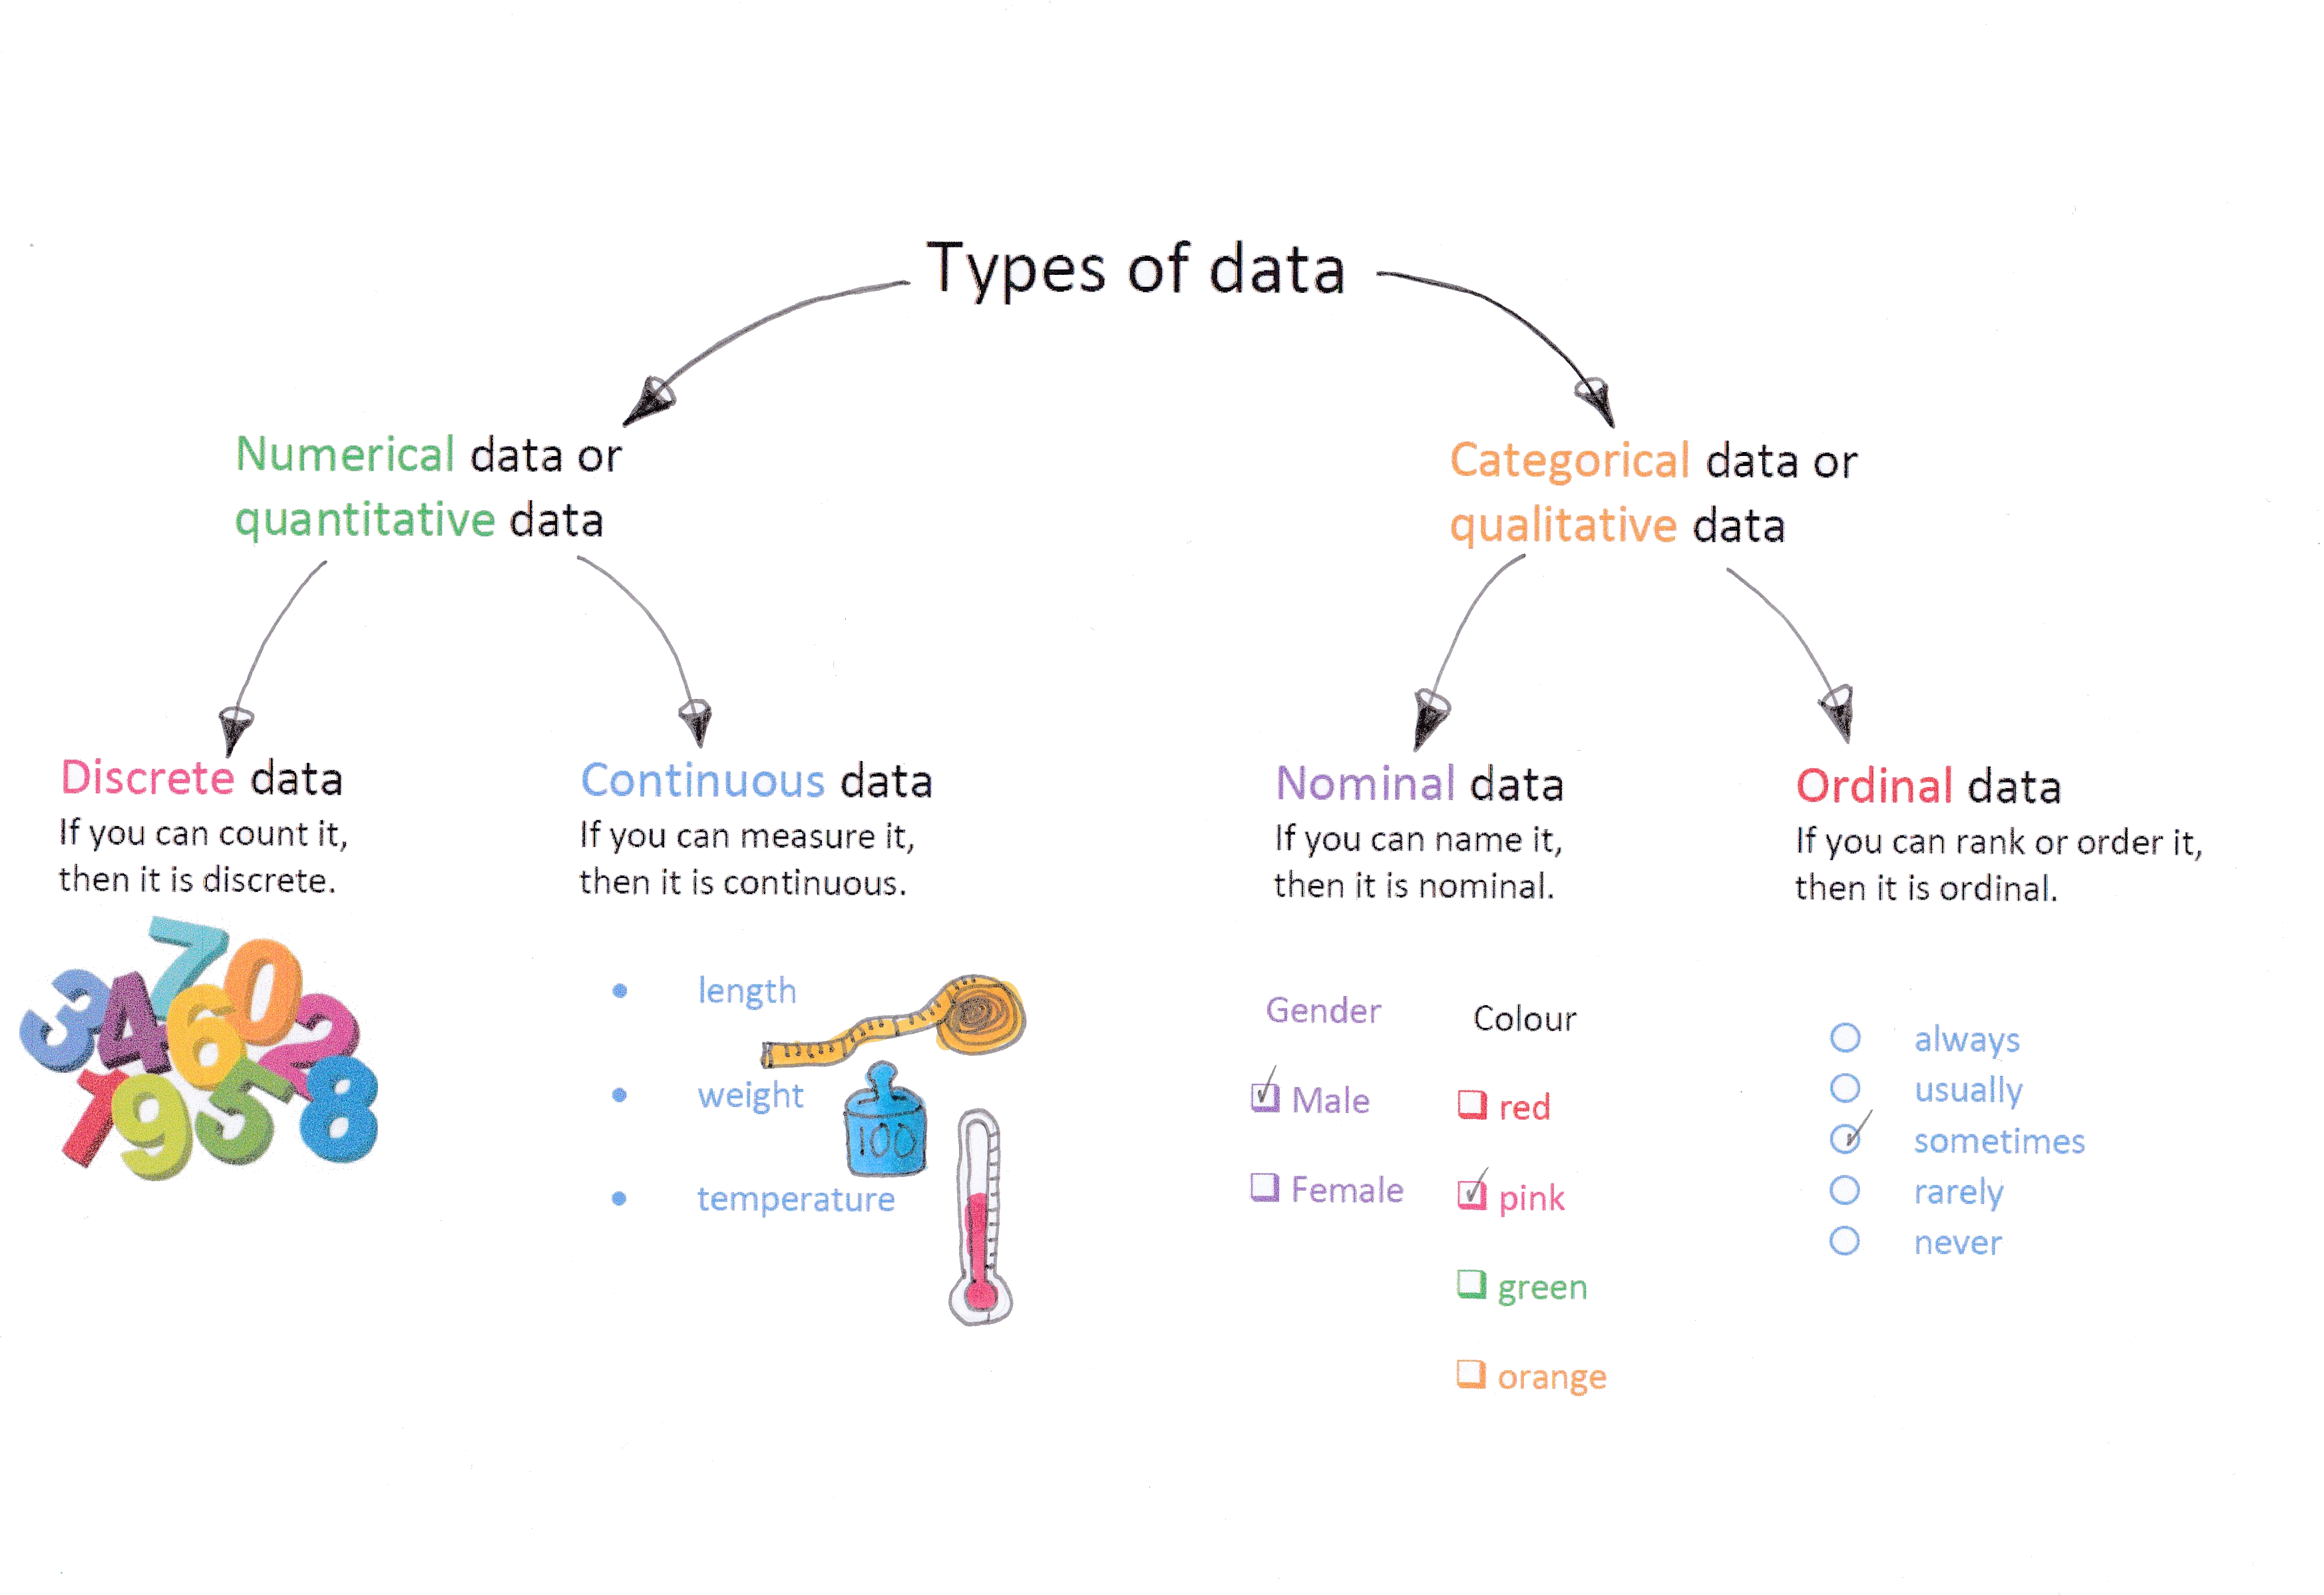
\includegraphics[width = 0.75\textwidth]{datatypes.png}}
\caption{Different data types}
\label{fig:dt}
\end{figure}


\subsection{Response Type}

The response variable is the variable of interest and the focus variable of the
hypothesis statement. The response variable can be classified as discrete or
continuous, typically measurements such as weight, height, temperature are all
considered to be continuous variables. Counts, scores and states which are
categories (alive/dead etc.) are discrete variables. The analysis method used
are dependent on the type of response variable. This includes choosing
appropriate graphical methods and the correct statistical model. A summary of
this information is in Table \ref{response}.

This workshop will focus on the analysis of continuous data using linear models
in it's various forms. Regression analysis is used where both the explanatory
variable and the response variable are continuous data types. ANOVA methods are
used where the explanatory variables are categorical in nature, analysis of
covariance is used where we have a mixture of continuous and categorical
explanatory variables. \clearpage

\small
\begin{table}[!hbp]
\begin{tabular}{|c|l|l|l|}
  \hline
  \textbf{Data} & \textbf{Example} & \textbf{Graphical} & \textbf{Statistical} \\
  \textbf{Type} & & \textbf{Techniques} & \textbf{Model} \\
  \hline
  \multirow{13}{*}{\rotatebox{90}{Discrete}} & \textbf{Counts - } & Column  & Generalised Linear Models  \\
           & faecal egg count  & or bar chart  & (GLM) with a Poisson \\
           & number of cells  &   &  distribution  \\
           & number of species  &  &  \\
  \cline{2-4}
           & \textbf{Scores - } &  Column & Sometimes analysed as \\
           & lodging &  or bar chart    & normal continuous data \\
           & disease score &  & ANOVA$^\ast$, linear models \\
           & zadoks &  & - but this might not be \\
           & &  & appropriate \\
  \cline{2-4}
           & \textbf{Categorical -}  &  Column & GLM - for example:   \\
           & dead/alive  &  or bar chart & logistic regression  \\
           & colour (red/blue/green)  &  &    \\
           & low/medium/high  &  &    \\
\hline
 \multirow{6}{*}{\rotatebox{90}{Continuous}} & \textbf{Measurements - } & Histogram & Linear models$^\ast$, including: \\
    & pH &  or Box plot & Simple Linear Regression\\
    & temperature & & Multiple Linear Regression\\
    & weight & & Polynomial Regression\\
    & height & & Analysis of Variance (ANOVA)\\
    & \% & & Analysis of Covariance\\
 \hline
    \multicolumn{4}{|c|}{$^\ast$  Transformations may be required to meet model assumptions}\\
 \hline
\end{tabular}
\caption{Response types with graphical \& statistical analysis methods.\label{response}}
\end{table}
\normalsize

It is important to be able to identify what data type of both the response and
explanatory variables. You need to consider this carefully before deciding
which type of analysis to pursue. Once you have decided on the type of analysis
that is appropriate for the data that you are working with, then it is
necessary to determine the ``best'' model to use; an understanding of the
experimental design used and the experimental and observations units is
essential.



\section{Commonly used designs}


The designs studied in W1 Planning and Designing Agronomic Experiments were:

\begin{itemize}
\item Completely Randomised Design (CRD)
\item Randomised Complete Block Design (RCBD)
\item Latin Square
\item Factorial Treatment Structures
\item Split-plot
\item Strip-plot
\end{itemize}

In this workshop we will consider the analysis of these experiments using the R statistical package \cite{r}.

\clearpage
\chapter{Linear models - Analysis of Variance}

\section{Completely Randomised Design (CRD)}
In a CRD the random allocation of treatments to experimental units is not constrained in any way. Usually the aim of
the analysis of this type of experiment is to determine whether treatment differences exist. The usual hypothesis test
is
\begin{eqnarray*}
	H_0&:& \mu_1 = \mu_2 = \hdots = \mu_t \\
	H_1&:& \texttt{not all treatment means are the same}
\end{eqnarray*}
For this analysis, if the null hypothesis is true, then all the treatments arise from a normal distribution with a
common mean (Figure \ref{fig:crdnull}). However, if the alternative hypothesis is true, the treatment are derived from
a set of normal distributions with a common variance where some or all of the means differ (Figure \ref{fig:crdalt}).
\begin{figure}[!hbtp]
\centering
\fbox{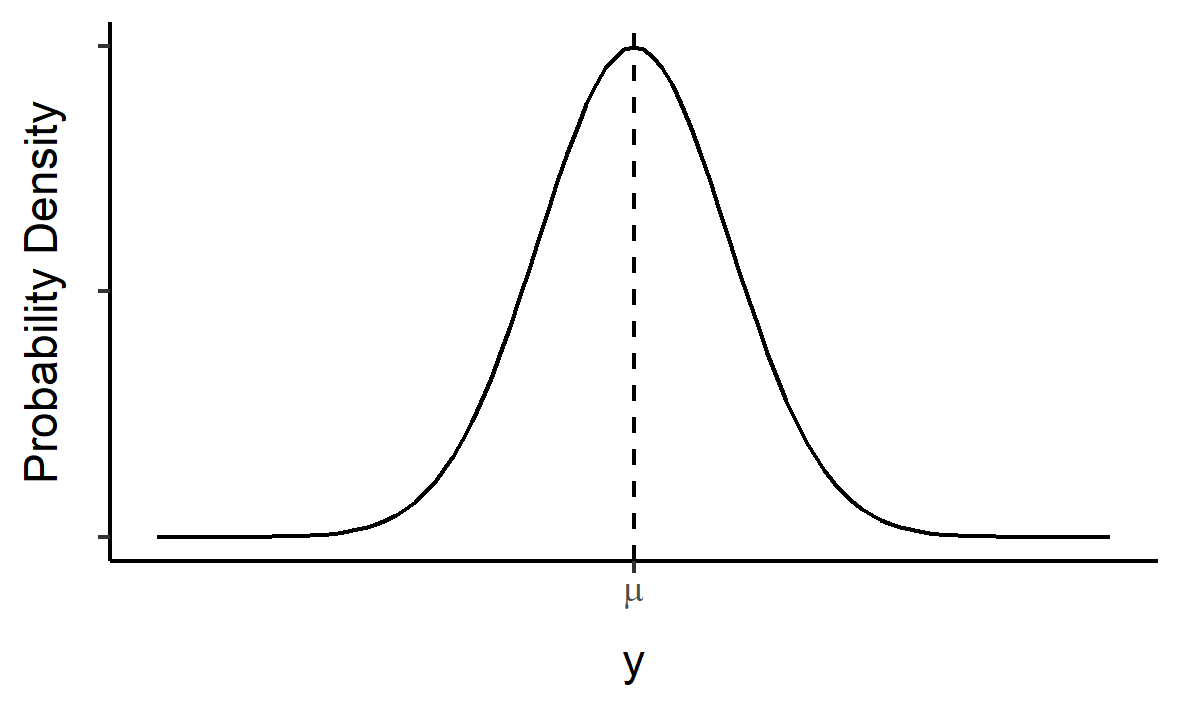
\includegraphics{CRDnullNormDensity.png}}
\caption{The assumed distribution under the null hypothesis}
\label{fig:crdnull}
\end{figure}
\clearpage
\begin{figure}[!hbtp]
\centering
\fbox{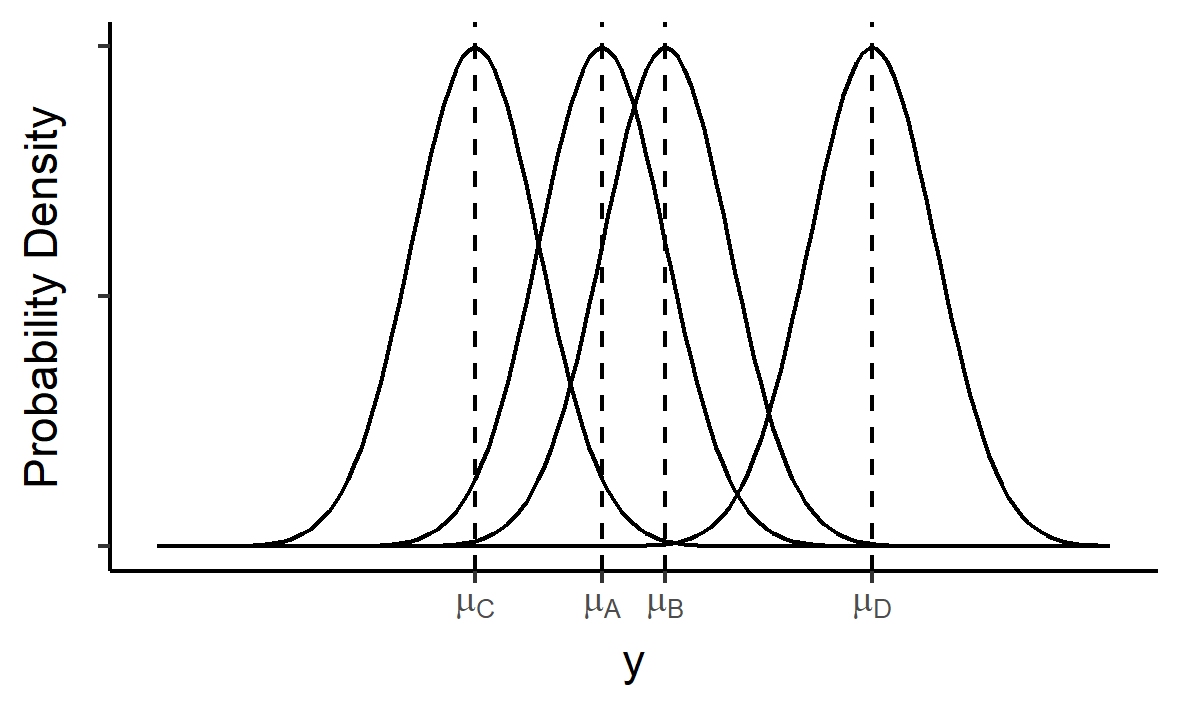
\includegraphics{CRDAlternativeNormDensity.png}}
\caption{The assumed distribution under the alternative hypothesis}
\label{fig:crdalt}
\end{figure}

\textbf{Exercise:}
\begin{table}[h]
\centering
\noindent\begin{tabular}{@{}*{1}{p{\textwidth}@{}}}
   \toprule
Draw two boxplot graphs depicting the Null and Alternative Hypotheses.
     \\
     \\
\textbf{Null Hypothesis - all the treatment means are equal}    \\
     \\
     \\
     \\
     \\
     \\
     \\
     \\
     \\
     \\
     \\
     \\
     \\
     \\
\textbf{Alternative Hypothesis - not all the treatment means are equal}    \\
     \\
     \\
     \\
     \\
     \\
     \\
     \\
     \\
     \\
     \\
     \\
     \\
     \\
\bottomrule
 \hline
\end{tabular}
\end{table}

\clearpage

The aim of Analysis of variance is to partition the variance of the response up into two or more parts. From the design
course we know that the skeletal ANOVA table for a CRD looks like:

\begin{verbatim}
Source of Variation                      df
=============================================
Treatment                                t-1
Residual                                 n-t
=============================================
Total                                    n-1
\end{verbatim}

where $t$ are the number of treatments and $n$ is the total number of responses. This ANOVA table shows that for a CRD
the variance is partitioned up into the variance that is associated with the treatments and the variance that is
associated with the residual or unexplained variance, as in Figure \ref{fig:crdbucket}.

\begin{figure}[!hbtp]
\centering
\fbox{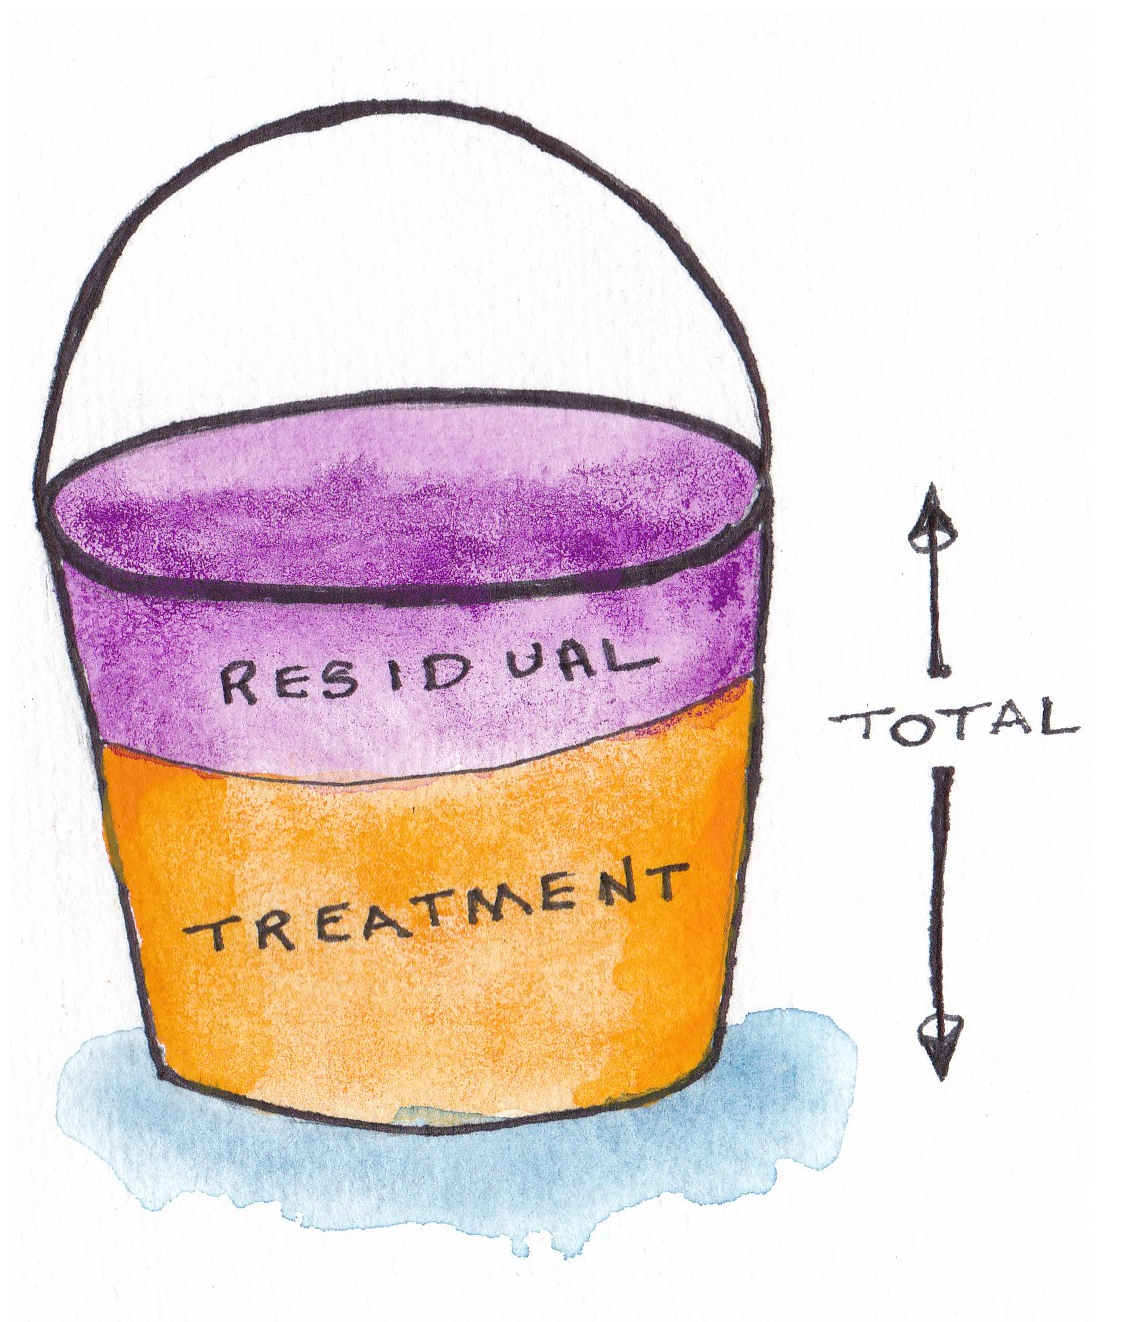
\includegraphics[width = 4cm]{crdbucket.png}}
\caption{Variance partitioning for a CRD}
\label{fig:crdbucket}
\end{figure}

If the variance associated with the treatment is much larger than the residual variance, the alternative hypothesis
will be supported by the model. To see how this works in practice a small example is used.

Consider a small hypothetical experiment based on a completely randomised design with three treatments and four
replicates. The data is provided in Table \ref{tab:hypcrd}

\begin{table}[ht]
\centering
\begin{tabular}{cc}
 \toprule
  treatment & response \\
  \midrule
  A & 4.28 \\
  A & 4.04 \\
  A & 4.67 \\
  A & 3.11 \\
  B & 6.29 \\
  B & 5.90 \\
  B & 7.21 \\
  B & 8.60 \\
  C & 6.17 \\
   C & 5.42 \\
   C & 5.85 \\
   C & 7.77 \\
   \bottomrule
\end{tabular}
\caption{\label{tab:hypcrd} Hypothetical data based on a completely randomised design.}
\end{table}

\clearpage

A graph of this data is shown in Figure \ref{fig:hypcrdbox}. We can see that there appears to be a difference in the
response for Treatment A compared to the other two treatments. Also, the spread of the treatments appears to be
similar.

\begin{figure}[!hbtp]
\centering
\fbox{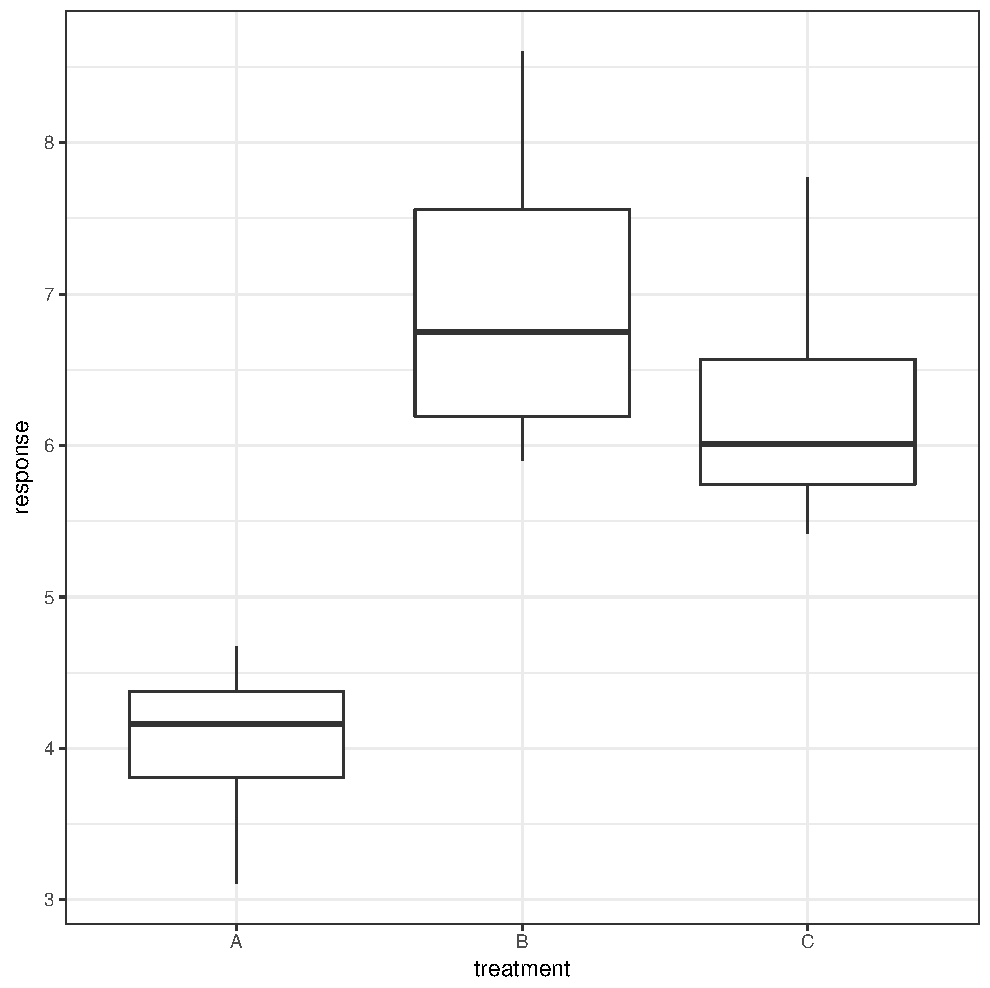
\includegraphics[width=0.6\textwidth]{hypcrd_boxplot.pdf}}
\caption{Hypothetical data based on a completely randomised design.}
\label{fig:hypcrdbox}
\end{figure}

The overall mean is simply the mean of all the responses, ignoring the treatments. Figure \ref{fig:hypcrdoverallmean}
shows the individual observations relative to the overall mean (gold horizontal line).


\begin{figure}[!hbtp]
\centering
\fbox{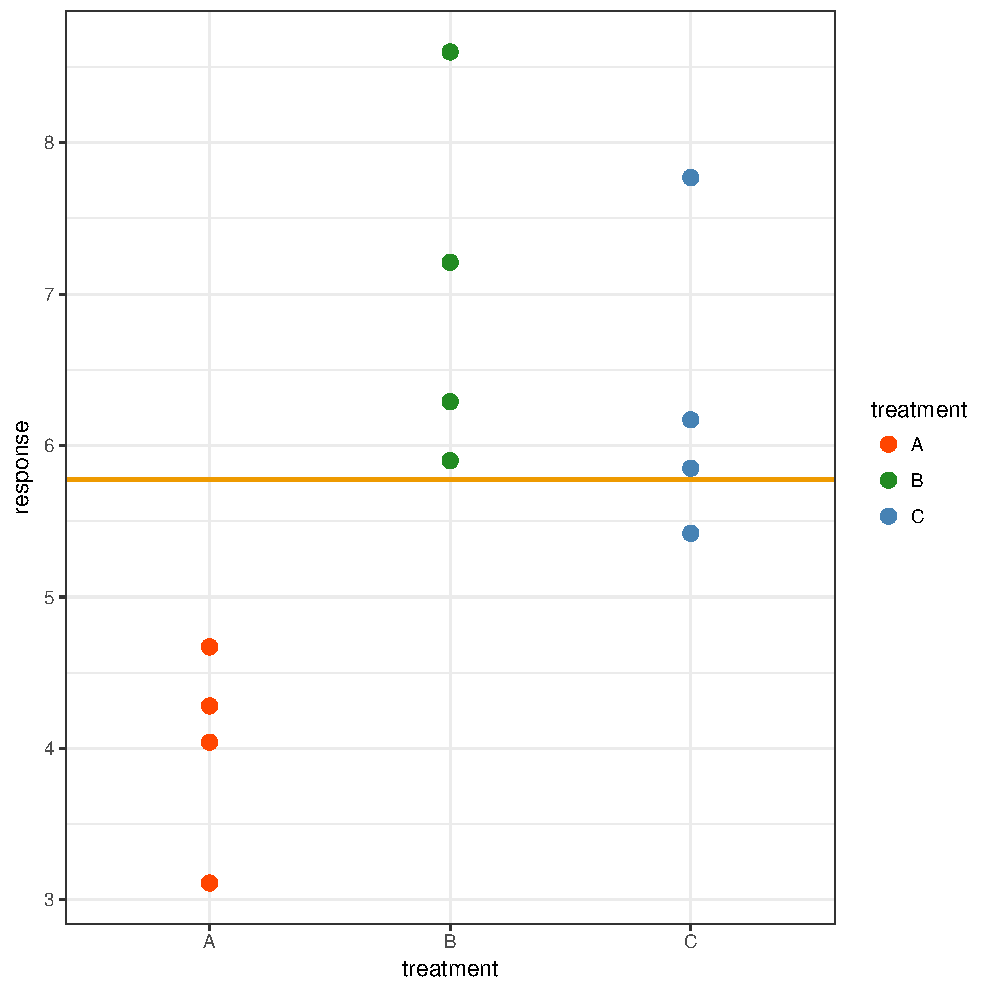
\includegraphics[width=0.6\textwidth]{hypcrd_overallmean.pdf}}
\caption{The observed data in relation to the overall mean.}
\label{fig:hypcrdoverallmean}
\end{figure}



The total variability associated with this data is based on the squared distances from the overall mean. Figure
\ref{fig:hypcrdtotss} shows the individual observations and the distances (in black) from the overall mean. These black
lines are representative of the total sums of squares.

\begin{figure}[!hbtp]
\centering
\fbox{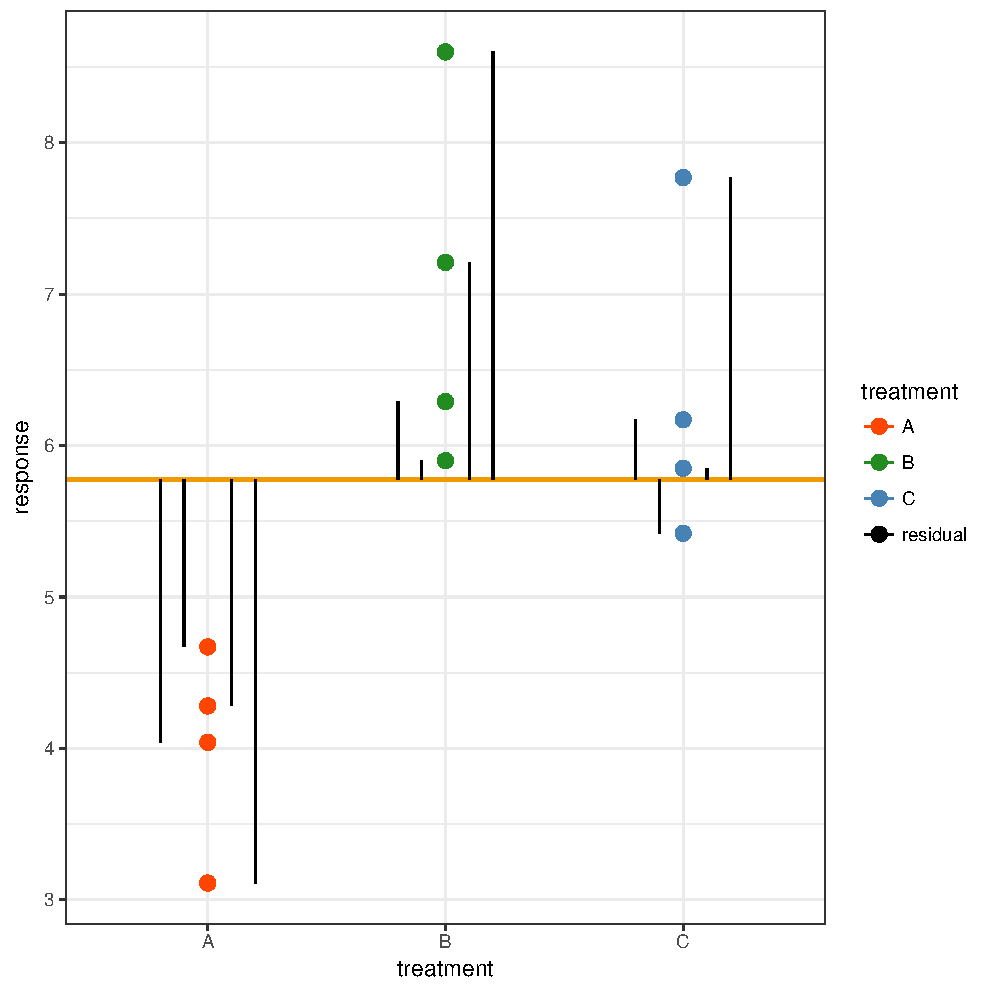
\includegraphics[width=0.6\textwidth]{hypcrd_totss.pdf}}
\caption{The observed data with representation of the total sums of squares.}
\label{fig:hypcrdtotss}
\end{figure}

In the analysis of a CRD, the total sums of squares is partitioned into the part that is associated with the treatments
and the remaining unexplained variance. When the model is fitted to the data the mean for each treatment is calculated.
The mean for each of the treatments in this example are shown in Figure \ref{fig:hypcrdtrtmean}.


\begin{figure}[!hbtp]
\centering
\fbox{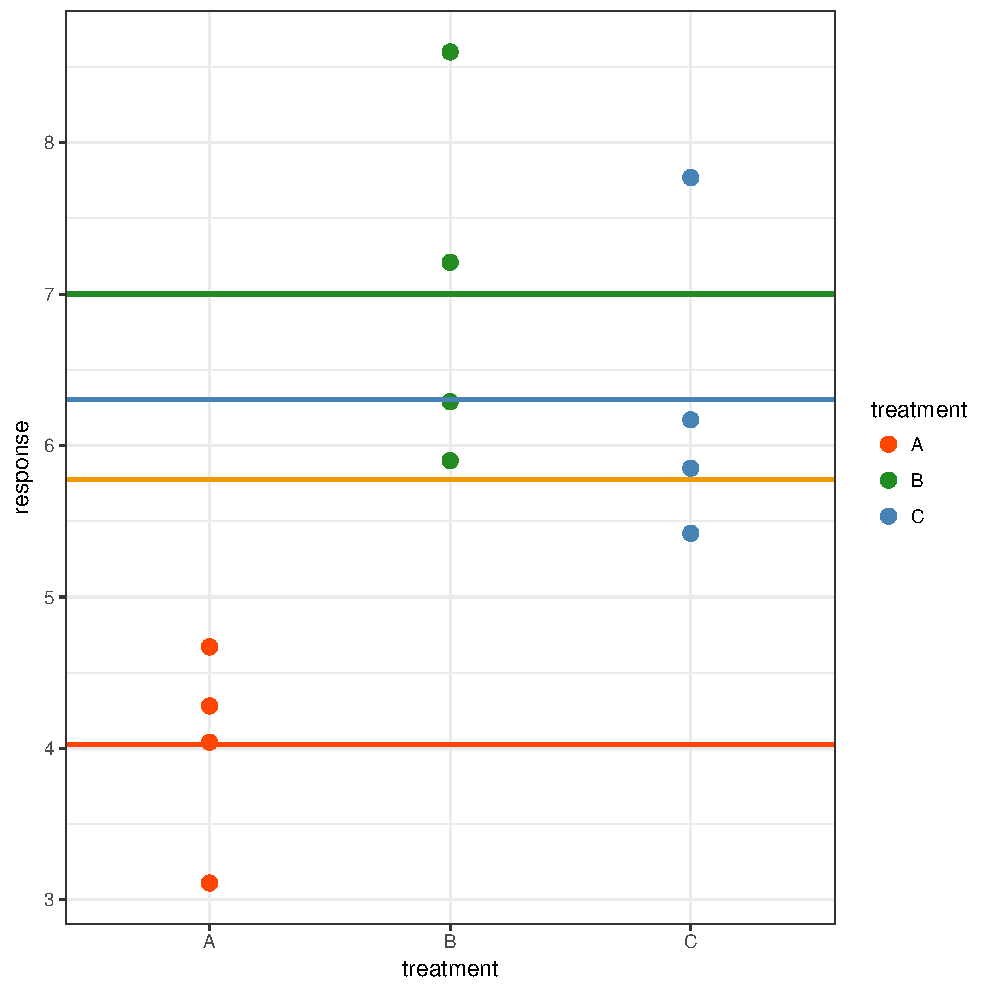
\includegraphics[width=0.6\textwidth]{hypcrd_trtmean.pdf}}
\caption{The observed data with treatment means.}
\label{fig:hypcrdtrtmean}
\end{figure}

The treatment sums of squares is the variability associated with this data is based on the squared distances from the
relative treatment mean. The treatment sum of squares is represented by the black vertical lines in Figure
\ref{fig:hypcrdtrtss}

\begin{figure}[!hbtp]
\centering
\fbox{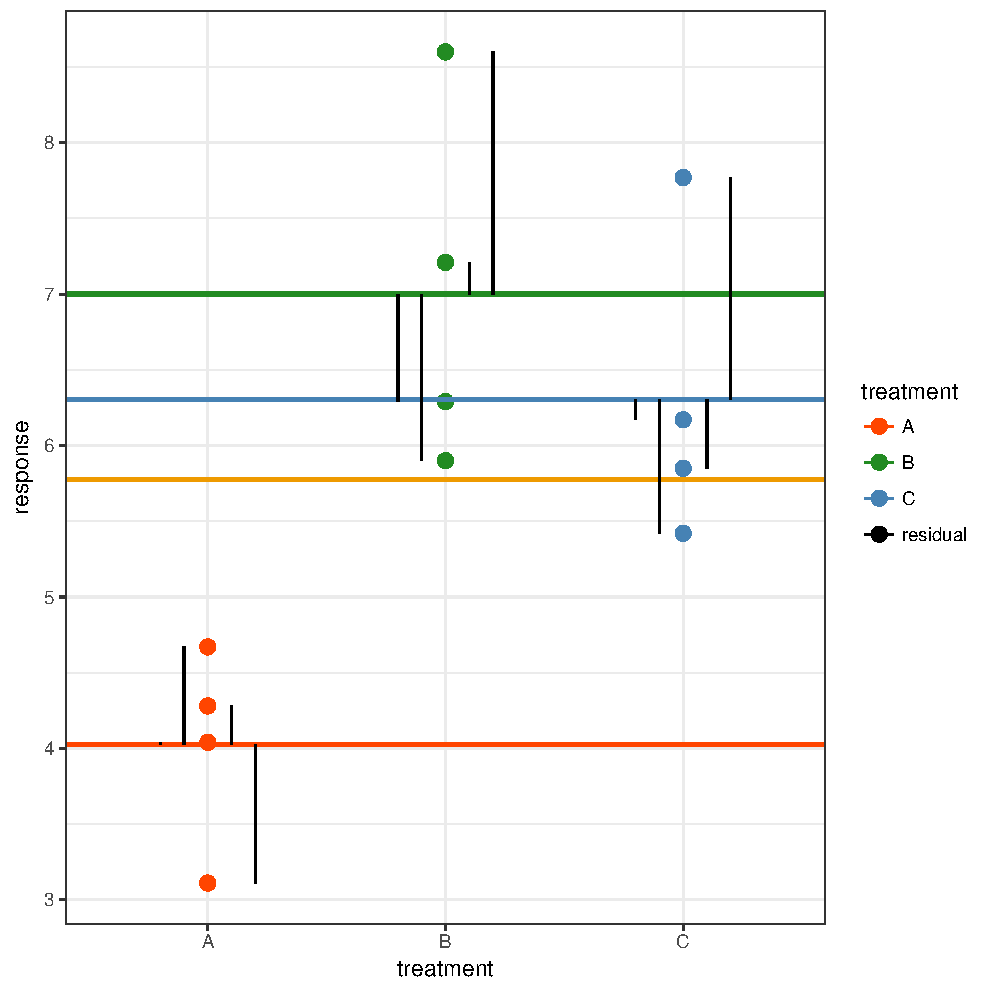
\includegraphics[width=0.6\textwidth]{hypcrd_trtss.pdf}}
\caption{The observed data with representation of the treatment sums of squares.}
\label{fig:hypcrdtrtss}
\end{figure}
\textbf{Note:} The distance from the overall mean to the treatment mean is called the effect of the treatment. An
effect is the difference between two means.


The ANOVA table (Table \ref{tab:crdaov}) is calculated as follows:

\begin{table}[ht]
\centering
\begin{tabular}{llllc}
\toprule
   & & & &\\
  Source & SS & df & MS & F \\
   & & & &\\
\midrule
   Treatment & $\sum\limits_{i=1}^{t}n_i(\bar{y}_{i}-\bar{y})^2$ & $t-1$ & $\frac{SS_{Trt}}{df_{Trt}}$ & $\frac{MS_{Trt}}{MS_{Residual}}$ \\
   & & & &\\
  Residual & $\sum\limits_{i=1}^{t} \sum\limits_{j=1}^{r} (y_{ij}-\bar{y}_{i})^2$ & $\sum\limits_{i=1}^{t}(n_i-t)$ & $\frac{SS_{Residual}}{df_{Residual}}$ &  \\
   & & & &\\
   Total & $\sum\limits_{i=1}^{t} \sum\limits_{j=1}^{r} (y_{ij}-\bar{y})^2 $ & $\sum\limits_{i=1}^{t}(n_i-1)$ &  &  \\
   & & & &\\
\bottomrule
\end{tabular}
\caption{\label{tab:crdaov} Single factor Analysis of Variance Table.}
\end{table}

where $y_{ij}$ represents the response from the $j^{th}$ observation on the $i^{th}$ treatment and the full set of
responses can be denoted as $y_{ij}$, $i = 1, \hdots , t$ and $j = 1, \hdots , r$.


We can see in Table \ref{tab:crdaov} that the $F$-value is calculated as the ratio of the variance associated with the
treatments to the variance associated with the residual. Typically $F$-values greater than 3 will show significance.
Figure \ref{fig:comp} shows how the boxplot and Sums of Squares partitioning may look under the null and alternative
hypothesis.


\begin{figure}[!hbtp]
\centering
\fbox{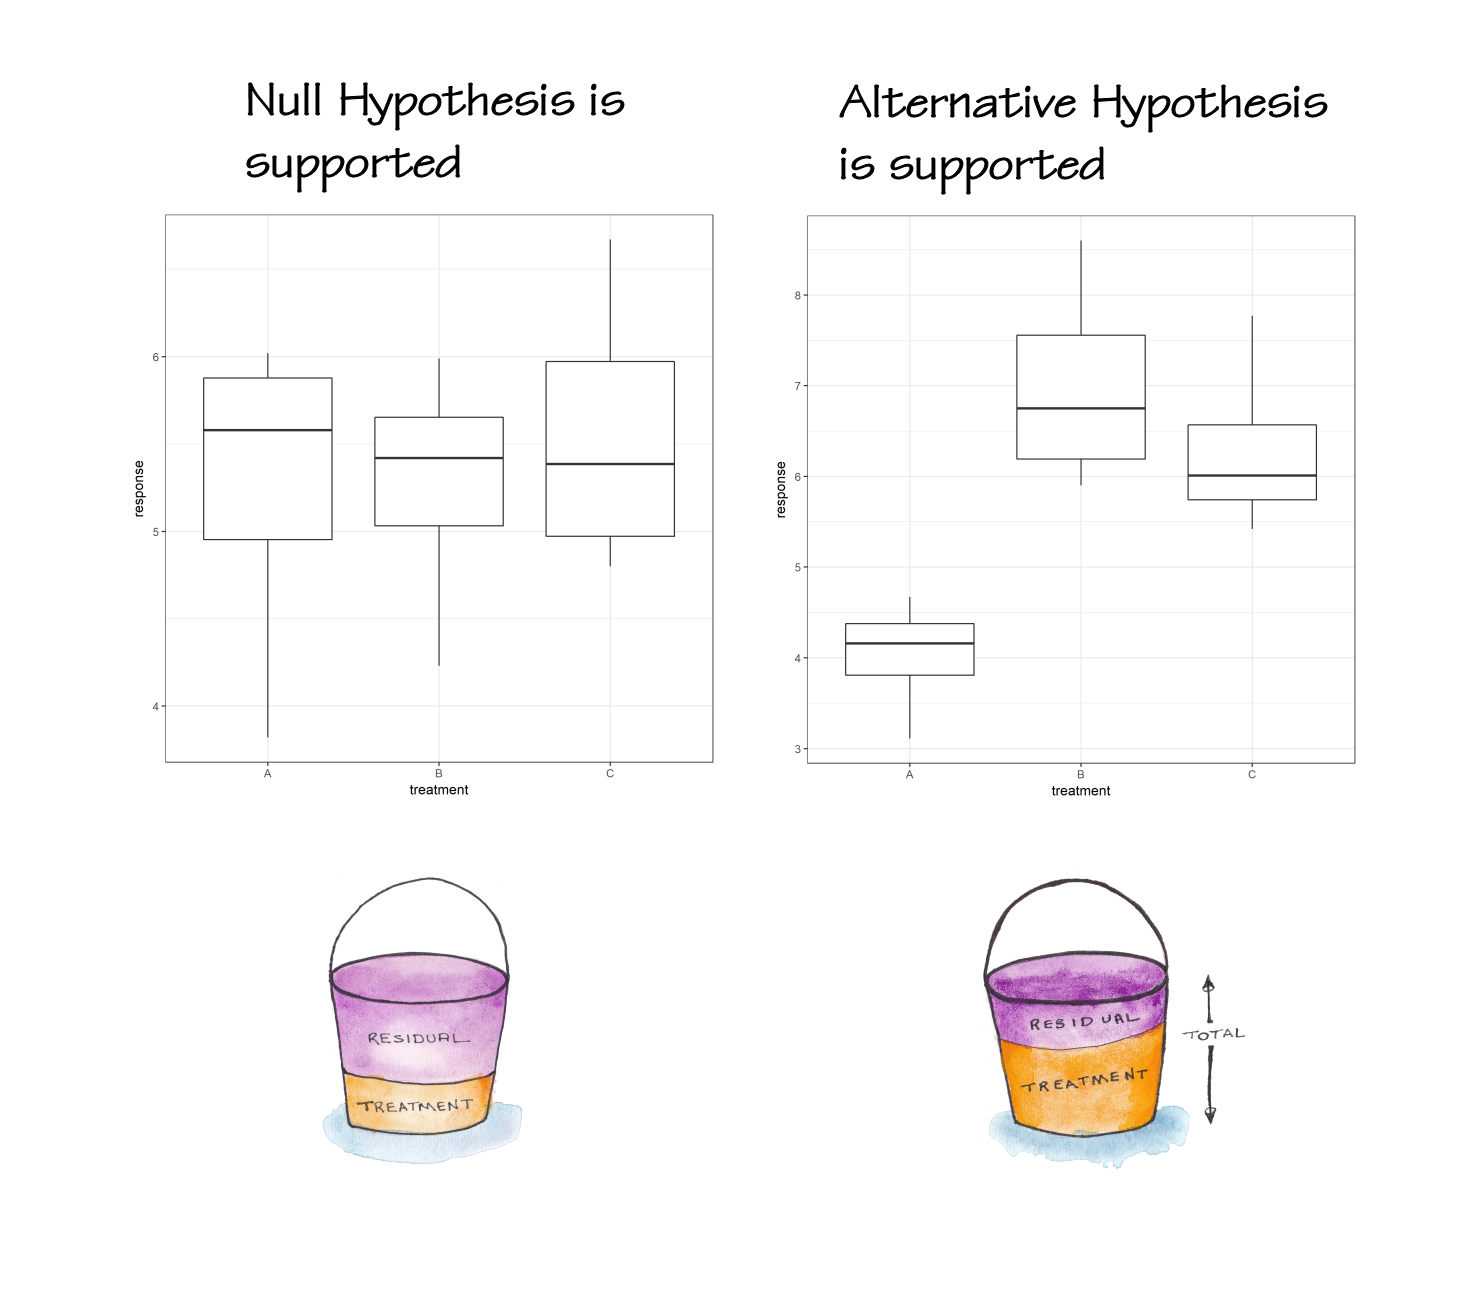
\includegraphics[width=0.8\textwidth]{compAcrd.png}}
\caption{Boxplot and Sums of Squares partitioning under the null and alternative hypothesis.}
\label{fig:comp}
\end{figure}

\textbf{Example 1}

An experiment was run to investigate the effect of the differences in soil
calcium on the root growth of plants. The experimental material consisted of 20
pots, each containing one plant, arranged in a rectangular array of four rows
and five columns, under uniform controlled conditions. The treatments comprised
four relative concentrations of calcium - 1, 5, 10 and 20. Each treatment was
applied to five pots selected at random to give a CRD design. The data can be
found in \texttt{example1.csv}.

\begin{application}{Experiment Layout Sketch}
\vspace{10cm}
\end{application}


The analysis will be undertaken to determine
\begin{eqnarray*}
	H_0&:& \mu_1 = \mu_5 = \mu_{10} = \mu_{20} \\
	H_1&:& \texttt{not all the calcium treatment means are the same}
\end{eqnarray*}

or this can be rewritten in terms of effects
\begin{eqnarray*}
	H_0&:& \alpha_1 = \alpha_5 = \alpha_{10} = \alpha_{20} = 0 \\
	H_1&:& \texttt{not all the calcium treatment effects are zero}
\end{eqnarray*}
These are identical hypotheses.

\subsection{Data Checking}


The first part of any analysis like this will be to visualise the data. We need to determine whether using usual
analysis of variance methods may be appropriate and check the data for any anomalies. When testing for the effect of a
treatment, a boxplot is an appropriate graph to use. The treatments are the $x$-variable and the response (root length)
is the dependent or $y$-variable.


The code to create the graph is given below:


\tcbset {colback = code!10!white, colframe = code}
\begin{tcolorbox}[title = Import and graph the data]
\begin{verbatim}
dat <- read.csv("example1.csv")                                # import the data
dat$trt <- factor(dat$trt)          # convert the treatment variable to a factor
\end{verbatim}
\tcblower
\begin{verbatim}
ggplot(data = dat, aes(x = trt, y = RL)) + geom_boxplot() + theme_bw()
\end{verbatim}
\end{tcolorbox}

\tcbset {colback = outpt!25!white, colframe = outpt}
\begin{tcolorbox}[title = Example 1 Boxplots of root length of plants for the concentrations of calcium ]
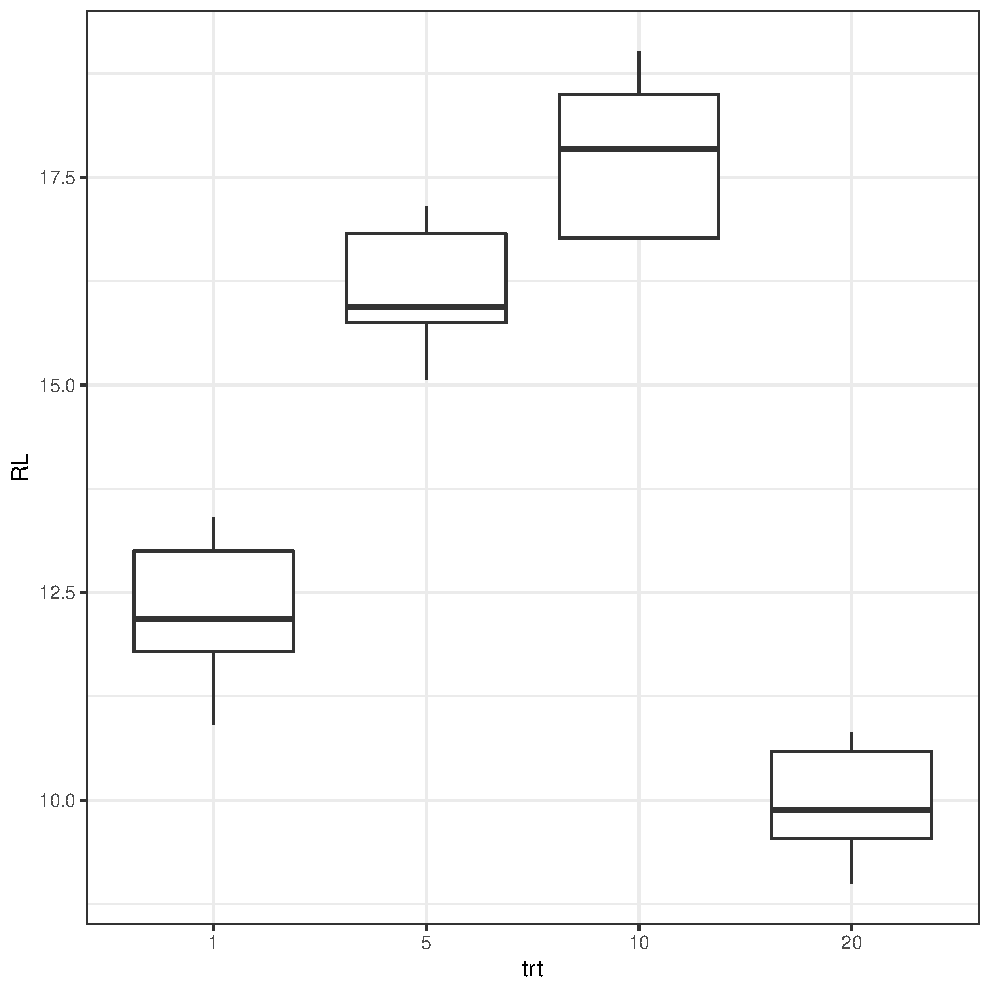
\includegraphics[width=0.8\textwidth, frame]{example1_boxplot.pdf}
\end{tcolorbox}


To interpret this graph the centre (median) and the spread are considered. Do the individual boxplots line up together
across the page? Or do they ``bounce'' up and down? This will help to understand the data while deciding whether to
expect the analysis of variance results to show a significant effect due to the treatments or not. The spread of each
boxplot (from the lowest point to the highest point) should be similar. This check is done in relation to the model
assumptions.

\subsection{Linear Model}

The linear model that is fit can be described by a simple model,

\begin{eqnarray*}
% \nonumber % Remove numbering (before each equation)
  RL_{ij} &=& \mu_i + \varepsilon_{ij}
\end{eqnarray*}

where $\mu_i$ is the true (but unknown) mean for the $i^{th}$ treatment and $\varepsilon_{ij}$ is the deviation
(residual) of the $j^{th}$ response on the $i^{th}$ treatment from its population mean.

Using symbolic notation, we can represent this equation as
\begin{eqnarray*}
	\texttt{Response variable}&:& \texttt{RL} \\
	\texttt{Explanatory component}&:& \texttt{Calcium Concentration}\\
	\texttt{Residual}&:& \texttt{Assume independence}
\end{eqnarray*}


\subsection{Model Assumptions}

\textbf{Assumption 1}
\begin{eqnarray*}
E(\varepsilon_{ij}) = 0
\end{eqnarray*}

This means that the population mean of the residuals is zero, which implies no systematic bias in the observations.

\textbf{Assumption 2}
\begin{eqnarray*}
Var(\varepsilon_{ij}) = \sigma^2
\end{eqnarray*}

The variances of the residuals are the same for all units. This is also known as homoscedasticity, or homogeneity of
variances.

\textbf{Assumption 3}
\begin{eqnarray*}
Cov(\varepsilon_{i},\varepsilon_{j}) = 0
\end{eqnarray*}

 The covariance between deviations for two separate observations is zero and the residuals are independent.

\textbf{Assumption 4}
\begin{eqnarray*}
\varepsilon_{ij} \sim \textsf{Normal}(0, \sigma^2)
\end{eqnarray*}

The residuals follow a Normal distribution with a mean 0 and variance $\sigma^2$.

\textbf{Assumption 5}

The values of the explanatory variables (factor or variates) are known without error.

The first three assumptions require that the residuals arise from the same
underlying probability distribution. The fourth assumption adds the requirement
that this is the Normal distribution, and this is necessary to make valid
statistical inferences that rely on the properties of the Normal distribution.
For the case of data with a single explanatory factor, Assumption 5 requires
that each observation can be allocated to a treatment group without error,
which is usually a realistic requirement.

\subsection{Fitting the Model}

Fitting the model is simply the physical process of running the model to analyse the data in a statistical package. In
this case we use the R statistical package \cite{r}. There are a number of different functions in R and other packages
that will allow the analysis of this experiment - for this analysis we will use the standard function \texttt{aov}.


\tcbset {colback = code!10!white, colframe = code}
\begin{tcolorbox}[title = Fitting the linear model for a CRD]
\begin{verbatim}
dat$trt <- factor(dat$trt)                      # convert trt to a factor

dat.aov <- aov(RL ~ trt, data = dat)            # fitting the model

\end{verbatim}

\tcblower
\begin{verbatim}
par(mfrow = c(2, 2))
plot(dat.aov)

anova(dat.aov)
\end{verbatim}
\end{tcolorbox}


\tcbset {colback = outpt!25!white, colframe = outpt}
\begin{tcolorbox}[title = Example 1 Output]
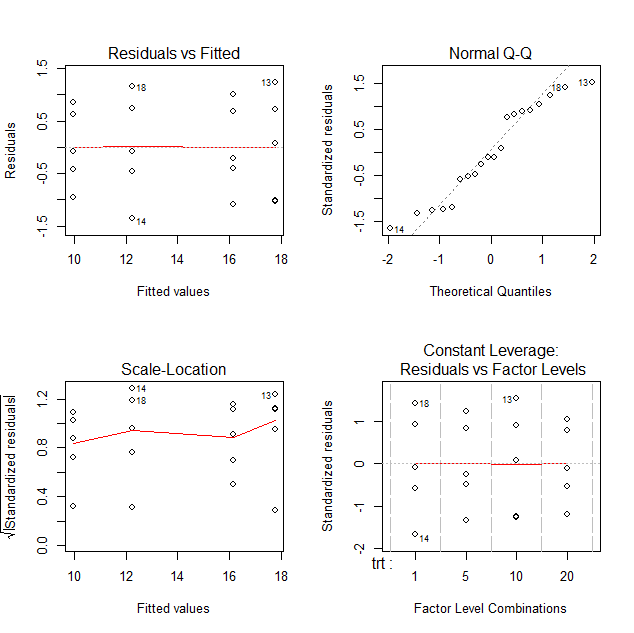
\includegraphics[width=0.8\textwidth, frame]{Example1Resplot.png}
\begin{verbatim}
Analysis of Variance Table

Response: RL
          Df Sum Sq Mean Sq F value    Pr(>F)
trt        3 190.79  63.598  77.675 9.414e-10 ***
Residuals 16  13.10   0.819
---
Signif. codes:  0 ‘***’ 0.001 ‘**’ 0.01 ‘*’ 0.05 ‘.’ 0.1 ‘ ’ 1
\end{verbatim}
\end{tcolorbox}


\subsection{Interpreting the Output}

The model assumptions need to be verified before the statistical inferences can be considered. Assumption 4 is assessed
using the first two graphs in the output (A and B) - the histogram and the QQ-plot. The histogram of the residuals
should be approximately symmetrical and bell-shaped, centred around zero. The QQ-plot displays the ordered residuals
plotted against the quantiles of the (in this case) Normal distribution. Deviations from the straight line indicates
deviation from the Normal distribution.

\tcbset {colback = interp!25!white, colframe = interp}
\begin{tcolorbox}[title = Example 1 Assumption 1]
\begin{verbatim}
When fitting an analysis of variance model as is done here Assumption 1
will always be true.
\end{verbatim}
\end{tcolorbox}


Assumption 2 is assessed using graph C - the residual plot. This plot should show approximately equal variance
(indicated by the vertical spread about zero) across the range of the fitted values.

\begin{tcolorbox}[title = Example 1 Assumption 2]
\begin{verbatim}
If the data have homogeneity of variances graph C should show
approximately equal variance across the range of the fitted values.

In this example there are four treatments so the four vertical lines
of residuals corresponds to the residuals associated with each of the
four treatments. The bigger the difference between the treatment means
the further spread the fitted values will be horizontally.

In this case the data show homogeneity of variances.
\end{verbatim}
\end{tcolorbox}

\begin{tcolorbox}[title = Example 1 Assumption 3]
\begin{verbatim}
Independence (Assumption 3) can safely be made given knowledge of the experimental
procedure. In this case we assume that the experiment was statistically designed
and run without complicating factors.
\end{verbatim}
\end{tcolorbox}

\begin{tcolorbox}[title = Example 1 Assumption 4]
\begin{verbatim}
Both the histogram and the QQ-plot show that the residuals follow an
approximate Normal distribution. There are only 20 observations in this
data, so it is not unusual that the histogram and QQ-plot are not exact.


The Shapiro-Wilk test of normality is used to determine if the residuals
are normally distributed.
\end{verbatim}
\end{tcolorbox}

\textbf{The Shapiro-Wilk test of normality}


The hypothesis being tested is:
\begin{align*}
& H_0: \text{The data are normally distributed}\\
& H_1: \text{The data are not normally distributed}\\
\end{align*}
and for the assumption the residuals are normally distributed to be met, the
p-value associated with the Shapiro-Wilk's test needs to be $\ge$ 0.05.


\tcbset {colback = code!10!white, colframe = code}
\begin{tcolorbox}[title = Testing Assumption 4 - Shapiro Wilk Test for Normality]
\begin{verbatim}
shapiro.test(dat.aov$residuals)
\end{verbatim}
\end{tcolorbox}
\clearpage

\tcbset {colback = outpt!25!white, colframe = outpt}
\begin{tcolorbox}[title = Example 1 Shapiro-Wilk normality test output]
\begin{verbatim}

        Shapiro-Wilk normality test

data:  dat.aov$residuals W = 0.92976, p-value = 0.1528
\end{verbatim}
\end{tcolorbox}


\tcbset {colback = interp!25!white, colframe = interp}
\begin{tcolorbox}[title = Example 1 Shapiro-Wilk normality test interpretation]
\begin{verbatim}

In this case we can conclude that the residuals are derived from a population
that is normally distributed (as the Shapiro-Wilk p-value = 0.1528).

\end{verbatim}
\end{tcolorbox}



\begin{tcolorbox}[title = Example 1 Assumption 5]
\begin{verbatim}
It is assumed that the treatments are allocated without error.
\end{verbatim}
\end{tcolorbox}

The model assumptions are met - it is valid to consider the results in the analysis of variance table.


Note: statistical packages display numbers in scientific notation as \texttt{9.41e-10}. This number is written in
scientific notation as $9.41\times 10^{-10}$.

\tcbset {colback = interp!25!white, colframe = interp}
\begin{tcolorbox}[title = Example 1 ANOVA interpretation]
\begin{verbatim}

The p value = 9.41e-10, which is less than 0.001 - highly significant,
and conclude there is evidence to suggest that not all the calcium
treatment means are the same.

\end{verbatim}
\end{tcolorbox}

There is evidence that the calcium level is affecting the root length of the plants. So the next step in the analysis
process is to find the means for each of the calcium treatments. In this simple case the simple means will be the same
as predicting the means based on the model but when a model is fitted to the data the predicted means (and standard
errors) should be presented.


\subsection{Prediction}

To get the predicted values when using the \texttt{aov} function, a data frame needs to be setup with the factor/s and
levels that predicted values are required. In this case we need a data frame with a single variable \texttt{trt}, with
the levels 1, 5, 10 and 20.

\tcbset {colback = code!10!white, colframe = code}
\begin{tcolorbox}[title = Example 1 predicted values]
\begin{verbatim}
library(emmeans)

pred.out <- emmeans(dat.aov, "trt")
pred.out
pred.out <- data.frame(pred.out)
\end{verbatim}
\end{tcolorbox}

\tcbset {colback = outpt!25!white, colframe = outpt}
\begin{tcolorbox}[title = Example 1 Predicted output]
\begin{verbatim}
 trt emmean        SE df  lower.CL upper.CL
 1   12.258 0.4046641 16 11.400151 13.11585
 5   16.144 0.4046641 16 15.286151 17.00185
 10  17.774 0.4046641 16 16.916151 18.63185
 20   9.964 0.4046641 16  9.106151 10.82185
\end{verbatim}
\end{tcolorbox}

As this is a simple design and analysis with equal replication the standard errors are the same for each treatment.
This will not always be the case.

\tcbset {colback = interp!25!white, colframe = interp}
\begin{tcolorbox}[title = Example 1 Prediction interpretation]
\begin{lstlisting}

Calcium concentration 10 has the highest predicted value of
17.8cm ($\pm$0.40cm) and Calcium concentration 20 has the
lowest predicted value of 10.0cm ($\pm$0.40cm).
\end{lstlisting}
\end{tcolorbox}


\subsection{Multiple Comparison Test}

The aim of this analysis was to determine the effect of the treatments. We have found a significant effect of treatment
on root length. When you want to determine the treatment differences you need to compare each treatment to every other
treatment. In the case where there are 4 treatments (as in Example 1), there are a total of 6 comparisons that need to
be made, to compare each treatment with all the other treatments - for more treatments many more comparisons are
required. In this situation it has been shown that the Type I error can be seriously compromised and the Type I error
for all the comparisons can end up being larger than expected. To adjust for this a \textbf{family-wise} Type I error
rate is employed and the method of comparison is called Tukey's Multiple Comparison Test.

When using the \texttt{aov} function we employ a function from the \texttt{agricolae} package (the same package we used
for designing the experiment).

\tcbset {colback = code!10!white, colframe = code}
\begin{tcolorbox}[title = Example 1 Tukey's multiple comparison]
\begin{verbatim}
library(agricolae)

tuk.out <- HSD.test(dat.aov, trt = "trt", console = TRUE)
tuk.out$groups$trt <- factor(row.names(tuk.out$groups),
                            levels = c("1", "5", "10", "20"))

library(dplyr)

pred.out <- left_join(pred.out, tuk.out$groups, by = "trt")
pred.out
\end{verbatim}
\end{tcolorbox}
\clearpage


\tcbset {colback = outpt!25!white, colframe = outpt}
\begin{tcolorbox}[title = Example 1 Tukey's multiple comparison output]
\begin{verbatim}
  trt emmean        SE df  lower.CL upper.CL     RL groups
1   1 12.258 0.4046641 16 11.400151 13.11585 12.258      b
2   5 16.144 0.4046641 16 15.286151 17.00185 16.144      a
3  10 17.774 0.4046641 16 16.916151 18.63185 17.774      a
4  20  9.964 0.4046641 16  9.106151 10.82185  9.964      c
\end{verbatim}
\end{tcolorbox}

\tcbset {colback = interp!25!white, colframe = interp}
\begin{tcolorbox}[title = Example 1 Prediction interpretation]
\begin{verbatim}
At the family 5% significance level:
- The two middle concentrations are not significantly different
- Calcium concentration 1 is significantly higher than concentration
             20 but significantly lower than concentrations 5 and 10.
- Calcium concentration 20 is significantly lower than all other concentrations
\end{verbatim}
\end{tcolorbox}

The means and standard errors from the predict and the ones provided by the \texttt{HSD.test} function are exactly the
same as expected. Saving the comparisons with the predicted values allow a graph of the predicted values to be made.

\tcbset {colback = code!10!white, colframe = code}
\begin{tcolorbox}[title = Example 1 Graph of predicted values]
\begin{verbatim}
# Calculate the upper and lower limits of the confidence intervals
pred.out$ci <-  qnorm(0.975)*pred.out$SE    #95% Confidence Interval
pred.out$low <- pred.out$emmean - pred.out$ci
pred.out$up <- pred.out$emmean + pred.out$ci

# graph the predicted values 
ggplot(data = pred.out, aes(x = trt)) +
geom_errorbar(aes(ymin = low, ymax = up), width = 0.2) +
geom_text(aes(x = trt, y = up, label = groups), vjust = 0, nudge_y = 0.1) +
geom_point(aes(y = emmean), color = "black", shape = 16) + theme_bw() +
labs(x = "Calcium Concentration", y = "Predicted Root Length (cm)")
\end{verbatim}
\end{tcolorbox}


\tcbset {colback = outpt!25!white, colframe = outpt}
\begin{tcolorbox}[title = Example 1 Graph of predicted values]
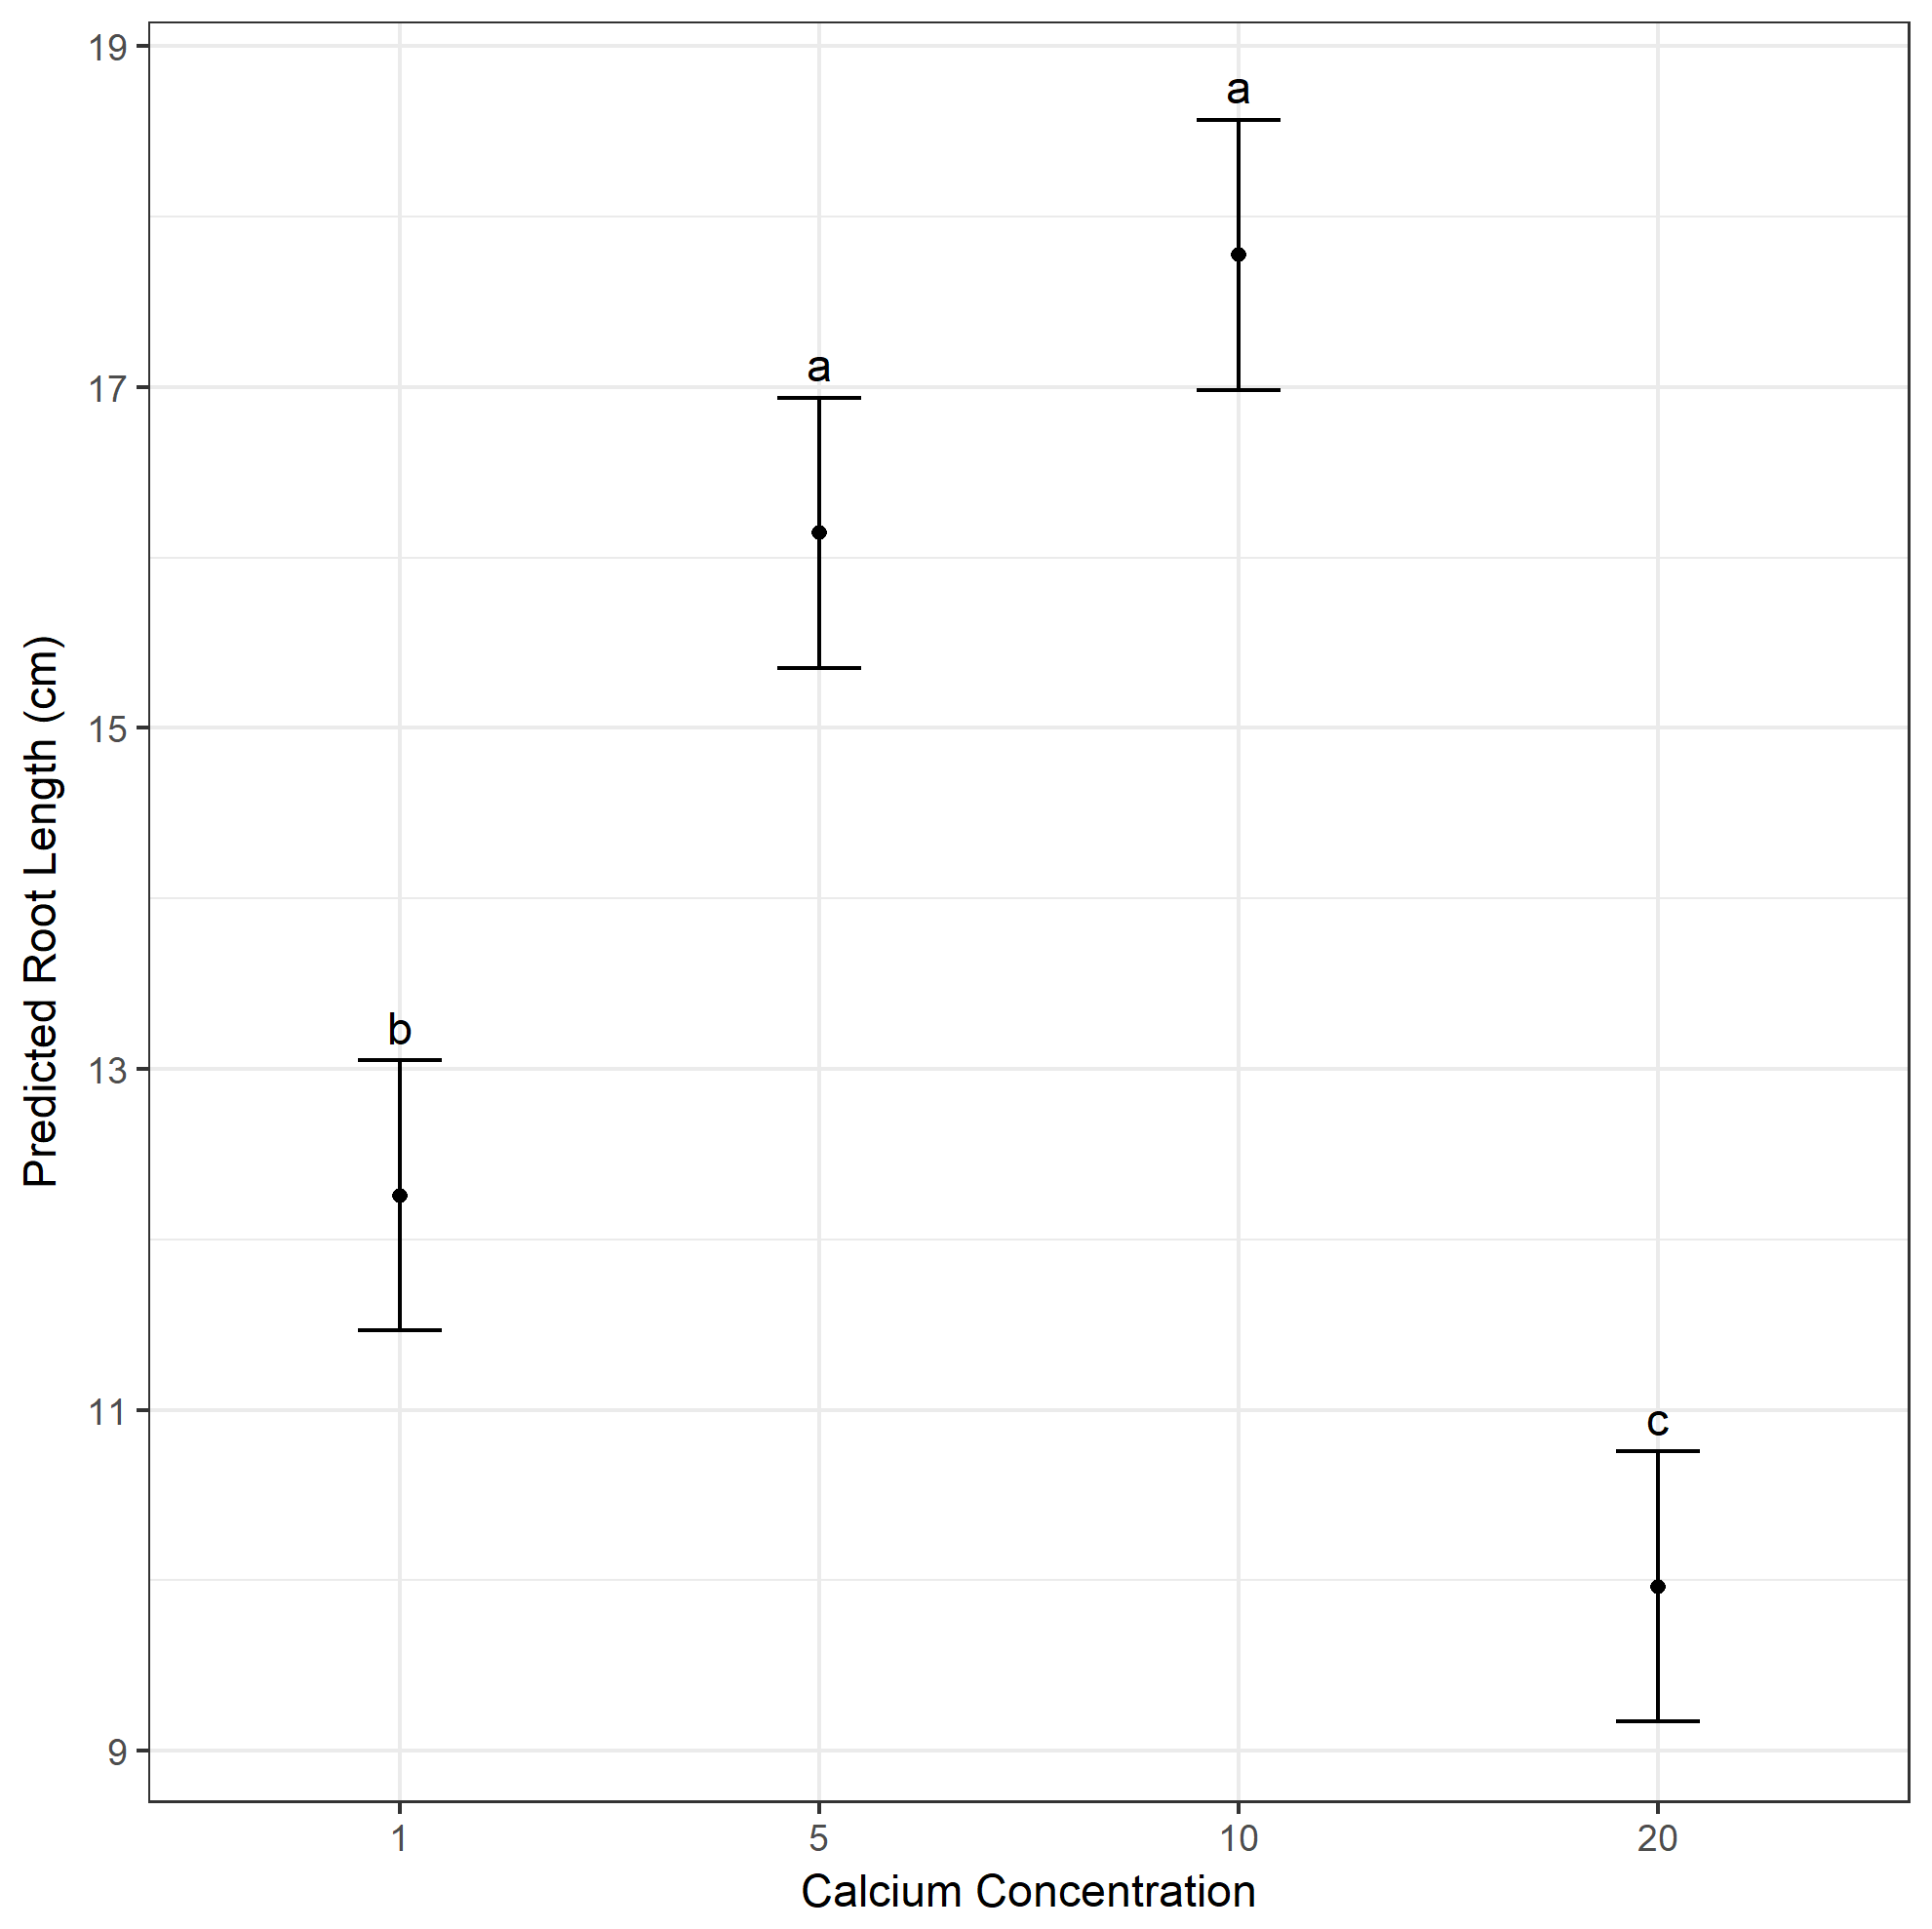
\includegraphics[width=0.8\textwidth, frame]{Example1Pred.png}
\end{tcolorbox}

\clearpage

\textbf{Example 2}

An experiment was run to investigate the effect of the differences in seven treatments in reducing scab disease in
potatoes. The experimental material consisted of 84 field plots arranged in a rectangular array of six rows and 14
columns. Each treatment was applied to 12 plots selected at random to give a CRD design. The response is the average
tuber length growth over a seven day period. The data can be found in \texttt{example2.csv}.


\begin{application}{Experiment Layout Sketch}
\vspace{10cm}
\end{application}


The analysis will be undertaken to determine
\begin{eqnarray*}
	H_0&:& \mu_{T1} = \mu_{T2} = \hdots = \mu_{T7} \\
	H_1&:& \texttt{not all the treatment means are the same}
\end{eqnarray*}
\subsection{Data Checking}
The code to create the boxplot is given below:


\tcbset {colback = code!10!white, colframe = code}
\begin{tcolorbox}[title = Import and graph the data]
\begin{verbatim}
dat <- read.csv("example2.csv")                                # import the data
dat$trt <- factor(dat$trt)          # convert the treatment variable to a factor
\end{verbatim}
\tcblower
\begin{verbatim}
ggplot(data = dat, aes(x = trt, y = TuberLengthGrowth)) + geom_boxplot() +
theme_bw() + labs(y = "Growth in Tuber Length (mm)", x = NULL)
\end{verbatim}
\end{tcolorbox}

\tcbset {colback = outpt!25!white, colframe = outpt}
\begin{tcolorbox}[title = Example 2 Boxplots of growth in tuber length for the treatments]
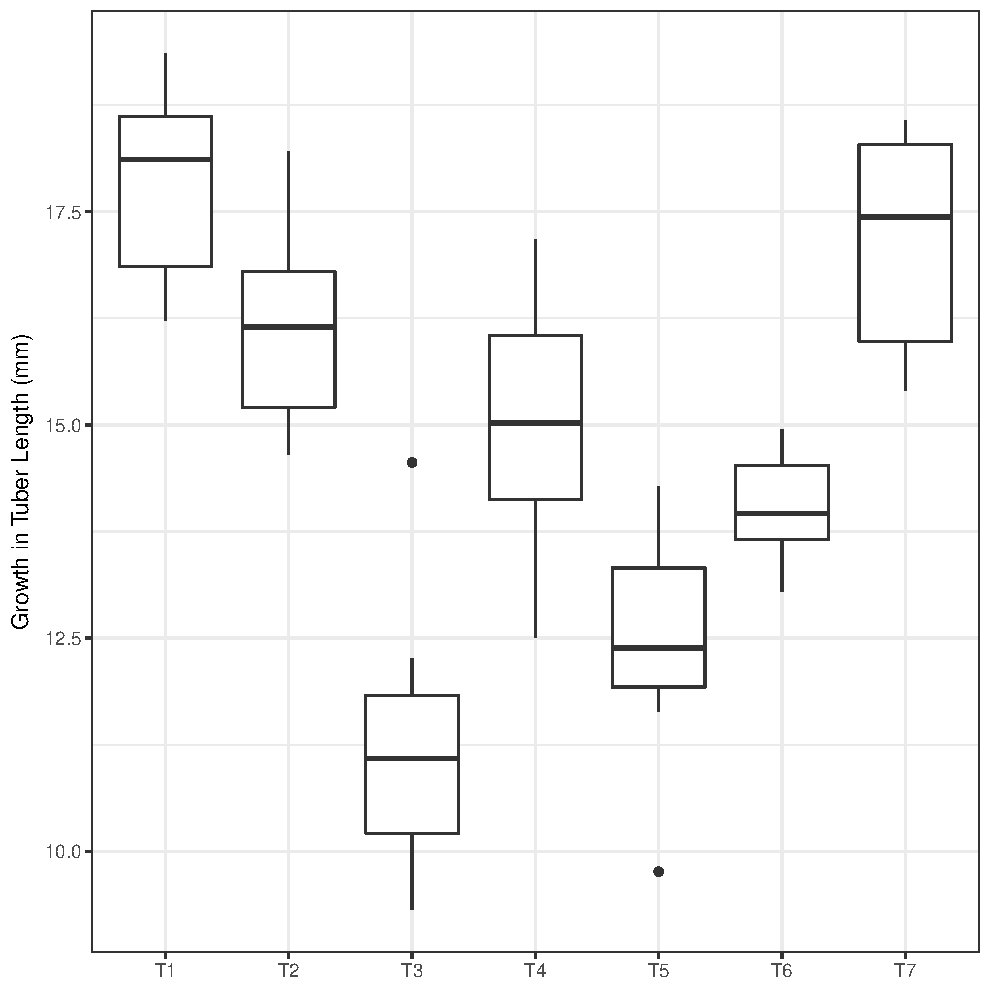
\includegraphics[width=0.8\textwidth, frame]{example2_boxplot.pdf}
\end{tcolorbox}
\clearpage
\subsection{Linear Model}

Using symbolic notation, the linear model is represented  as
\begin{eqnarray*}
	\texttt{Response variable}&:& \texttt{Tuber Length Growth} \\
	\texttt{Explanatory component}&:& \texttt{Treatment}\\
	\texttt{Residual}&:& \texttt{Assume independence}
\end{eqnarray*}


\subsection{Fitting the Model}

\tcbset {colback = code!10!white, colframe = code}
\begin{tcolorbox}[title = Fitting the linear model for a CRD]
\begin{verbatim}
dat$trt <- factor(dat$trt)                      # convert trt to a factor

dat.aov <- aov(TuberLengthGrowth ~ trt, data = dat)   # fitting the model

\end{verbatim}

\tcblower
\begin{verbatim}
par(mfrow = c(2, 2))
plot(dat.aov)
anova(dat.aov)
shapiro.test(dat.aov$residuals)
\end{verbatim}
\end{tcolorbox}

\tcbset {colback = outpt!25!white, colframe = outpt}
\begin{tcolorbox}[title = Example 2 Output]
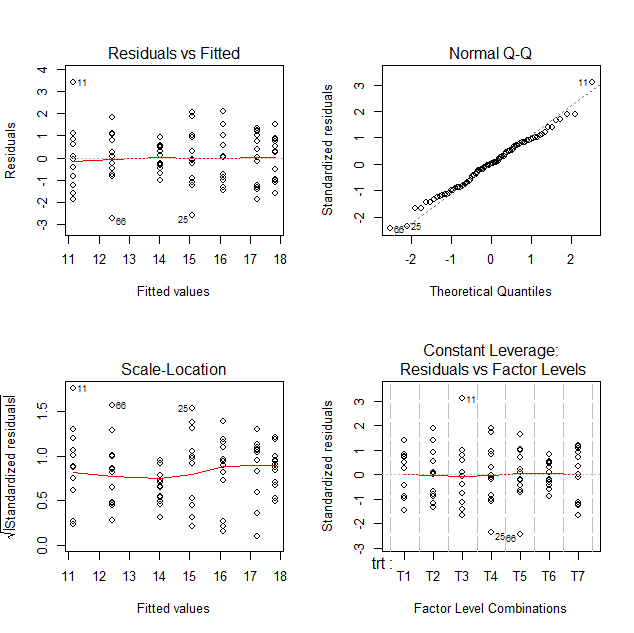
\includegraphics[width=0.8\textwidth, frame]{Example2Resplot.png}
\end{tcolorbox}

\begin{tcolorbox}[title = Example 2 Output]
\begin{verbatim}
Analysis of Variance Table

Response: TuberLengthGrowth
          Df Sum Sq Mean Sq F value    Pr(>F)
trt        6 436.01  72.668  54.989 < 2.2e-16 ***
Residuals 77 101.76   1.322
---
Signif. codes:  0 ‘***’ 0.001 ‘**’ 0.01 ‘*’ 0.05 ‘.’ 0.1 ‘ ’ 1

\end{verbatim}
\end{tcolorbox}


\subsection{Interpreting the Output}

The model assumptions need to be verified before the statistical inferences can be considered. Assumption 4 is assessed
using the first two graphs in the output (A and B) - the histogram and the QQ-plot. The histogram of the residuals
should be approximately symmetrical and bell-shaped, centred around zero. The QQ-plot displays the ordered residuals
plotted against the quantiles of the (in this case) Normal distribution. Deviations from the straight line indicates
deviation from the Normal distribution.

\tcbset {colback = interp!25!white, colframe = interp}
\begin{tcolorbox}[title = Example 2 Assumption 1]
\begin{verbatim}
When fitting an analysis of variance model as is done here Assumption 1
will always be true.
\end{verbatim}
\end{tcolorbox}


Assumption 2 is assessed using graph C - the residual plot. This plot should show approximately equal variance
(indicated by the vertical spread about zero) across the range of the fitted values.

\begin{tcolorbox}[title = Example 2 Assumption 2]
\begin{verbatim}
If the data have homogeneity of variances graph C should show
approximately equal variance across the range of the fitted values.

In this case the data show homogeneity of variances.
\end{verbatim}
\end{tcolorbox}

\begin{tcolorbox}[title = Example 2 Assumption 3]
\begin{verbatim}
Independence (Assumption 3) can safely be made given knowledge of the experimental
procedure. In this case we assume that the experiment was statistically designed
and run without complicating factors.
\end{verbatim}
\end{tcolorbox}

\begin{tcolorbox}[title = Example 2 Assumption 4]
\begin{verbatim}
Both the histogram and the QQ-plot show that the residuals follow an
approximate Normal distribution.

The Shapiro-Wilk test of normality is used to determine if the residuals
are normally distributed.
\end{verbatim}
\end{tcolorbox}

\tcbset {colback = outpt!25!white, colframe = outpt}
\begin{tcolorbox}[title = Example 2 Shapiro-Wilk normality test output]
\begin{verbatim}
        Shapiro-Wilk normality test

data:  dat.aov$residuals
W = 0.99165, p-value = 0.8718
\end{verbatim}
\end{tcolorbox}


\tcbset {colback = interp!25!white, colframe = interp}
\begin{tcolorbox}[title = Example 2 Shapiro-Wilk normality test interpretation]
\begin{verbatim}

In this case we can conclude that the residuals are derived from a population
that is normally distributed (as the Shapiro-Wilk p-value =0.8718).

\end{verbatim}
\end{tcolorbox}



\begin{tcolorbox}[title = Example2 Assumption 5]
\begin{verbatim}
It is assumed that the treatments are allocated without error.
\end{verbatim}
\end{tcolorbox}

The model assumptions are met - it is valid to consider the results in the analysis of variance table.

\tcbset {colback = interp!25!white, colframe = interp}
\begin{tcolorbox}[title = Example 2 ANOVA interpretation]
\begin{verbatim}

The p value = 2.2e-16, which is less than 0.001 - highly significant,
and conclude there is evidence to suggest that not all the treatment
means are the same.

\end{verbatim}
\end{tcolorbox}
\subsection{Prediction}

\tcbset {colback = code!10!white, colframe = code}
\begin{tcolorbox}[title = Example 2 predicted values]
\begin{verbatim}
library(emmeans)

pred.out <- emmeans(dat.aov, "trt")
pred.out
pred.out <- data.frame(pred.out)
\end{verbatim}
\end{tcolorbox}

\tcbset {colback = outpt!25!white, colframe = outpt}
\begin{tcolorbox}[title = Example 2 Predicted output]
\begin{verbatim}
 trt   emmean        SE df lower.CL upper.CL
 T1  17.82917 0.3318526 77 17.16836 18.48997
 T2  16.11167 0.3318526 77 15.45086 16.77247
 T3  11.15250 0.3318526 77 10.49170 11.81330
 T4  15.10083 0.3318526 77 14.44003 15.76164
 T5  12.45417 0.3318526 77 11.79336 13.11497
 T6  14.02500 0.3318526 77 13.36420 14.68580
 T7  17.24000 0.3318526 77 16.57920 17.90080
\end{verbatim}
\end{tcolorbox}

\tcbset {colback = interp!25!white, colframe = interp}
\begin{tcolorbox}[title = Example 2 Prediction interpretation]
\begin{lstlisting}

Treatment T3 has the lowest predicted value of 11.2mm ($\pm$0.33mm)
and T1 has the highest predicted value of 17.8mm
($\pm$0.33cm).
\end{lstlisting}
\end{tcolorbox}


\subsection{Multiple Comparison Test}

\tcbset {colback = code!10!white, colframe = code}
\begin{tcolorbox}[title = Example 2 Tukey's multiple comparison]
\begin{verbatim}
library(agricolae)

tuk.out <- HSD.test(dat.aov, trt = "trt", console = TRUE)
tuk.out$groups$trt <- factor(row.names(tuk.out$groups))

library(dplyr)

pred.out <- left_join(pred.out, tuk.out$groups, by = "trt")
pred.out
\end{verbatim}
\end{tcolorbox}
\clearpage


\tcbset {colback = outpt!25!white, colframe = outpt}
\begin{tcolorbox}[title = Example 2 Tukey's multiple comparison output]
\begin{verbatim}
Study: dat.aov ~ "trt"

HSD Test for TuberLengthGrowth

Mean Square Error:  1.321514

trt,  means

   TuberLengthGrowth       std  r   Min   Max
T1          17.82917 0.9911835 12 16.23 19.36
T2          16.11167 1.1392967 12 14.65 18.21
T3          11.15250 1.4232557 12  9.31 14.56
T4          15.10083 1.3563417 12 12.51 17.18
T5          12.45417 1.1768638 12  9.76 14.28
T6          14.02500 0.5815418 12 13.04 14.95
T7          17.24000 1.1754303 12 15.40 18.57

Alpha: 0.05 ; DF Error: 77
Critical Value of Studentized Range: 4.28176

Minimum Significant Difference: 1.420913

Treatments with the same letter are not significantly different.

   TuberLengthGrowth groups
T1          17.82917      a
T7          17.24000     ab
T2          16.11167     bc
T4          15.10083     cd
T6          14.02500      d
T5          12.45417      e
T3          11.15250      e
\end{verbatim}
\tcblower
\begin{verbatim}
  trt   emmean        SE df lower.CL upper.CL TuberLengthGrowth groups
1  T1 17.82917 0.3318526 77 17.16836 18.48997          17.82917      a
2  T2 16.11167 0.3318526 77 15.45086 16.77247          16.11167     bc
3  T3 11.15250 0.3318526 77 10.49170 11.81330          11.15250      e
4  T4 15.10083 0.3318526 77 14.44003 15.76164          15.10083     cd
5  T5 12.45417 0.3318526 77 11.79336 13.11497          12.45417      e
6  T6 14.02500 0.3318526 77 13.36420 14.68580          14.02500      d
7  T7 17.24000 0.3318526 77 16.57920 17.90080          17.24000     ab

\end{verbatim}
\end{tcolorbox}

\tcbset {colback = interp!25!white, colframe = interp}
\begin{tcolorbox}[title = Example 2 Prediction interpretation]
\begin{verbatim}
At the family 5% significance level:
- T1 and T7 are not significantly different but T1 is significantly higher than
the other treatments
- T2 is not significantly different from T4 or T7
- T3 is not significantly different T5
- T4 is not significantly different T2 or T6
- T6 is not significantly different T4
- T7 is not significantly different from T1 or T2
\end{verbatim}
\end{tcolorbox}
\tcbset {colback = code!10!white, colframe = code}
\begin{tcolorbox}[title = Example 2 Graph of predicted values]
\begin{verbatim}
# Calculate the upper and lower limits of the confidence intervals
pred.out$ci <-  qnorm(0.975)*pred.out$SE    #95% Confidence Interval
pred.out$low <- pred.out$emmean - pred.out$ci
pred.out$up <- pred.out$emmean + pred.out$ci

# order the treatment by growth
pred.out <- pred.out[order(pred.out$emmean),]
pred.out$trt <- factor(as.character(pred.out$trt),
                levels = as.character(pred.out$trt))
 
# graph the predicted values 
ggplot(data = pred.out, aes(x = trt)) +
geom_errorbar(aes(ymin = low, ymax = up), width = 0.2) +
geom_text(aes(x = trt, y = up, label = groups), vjust = 0, nudge_y = 0.1) +
geom_point(aes(y = emmean), color = "black", shape = 16) + theme_bw() +
labs(x = "Treatment", y = "Predicted Growth in Tuber Length (mm)")
\end{verbatim}
\end{tcolorbox}


\tcbset {colback = outpt!25!white, colframe = outpt}
\begin{tcolorbox}[title = Example 2 Graph of predicted values]
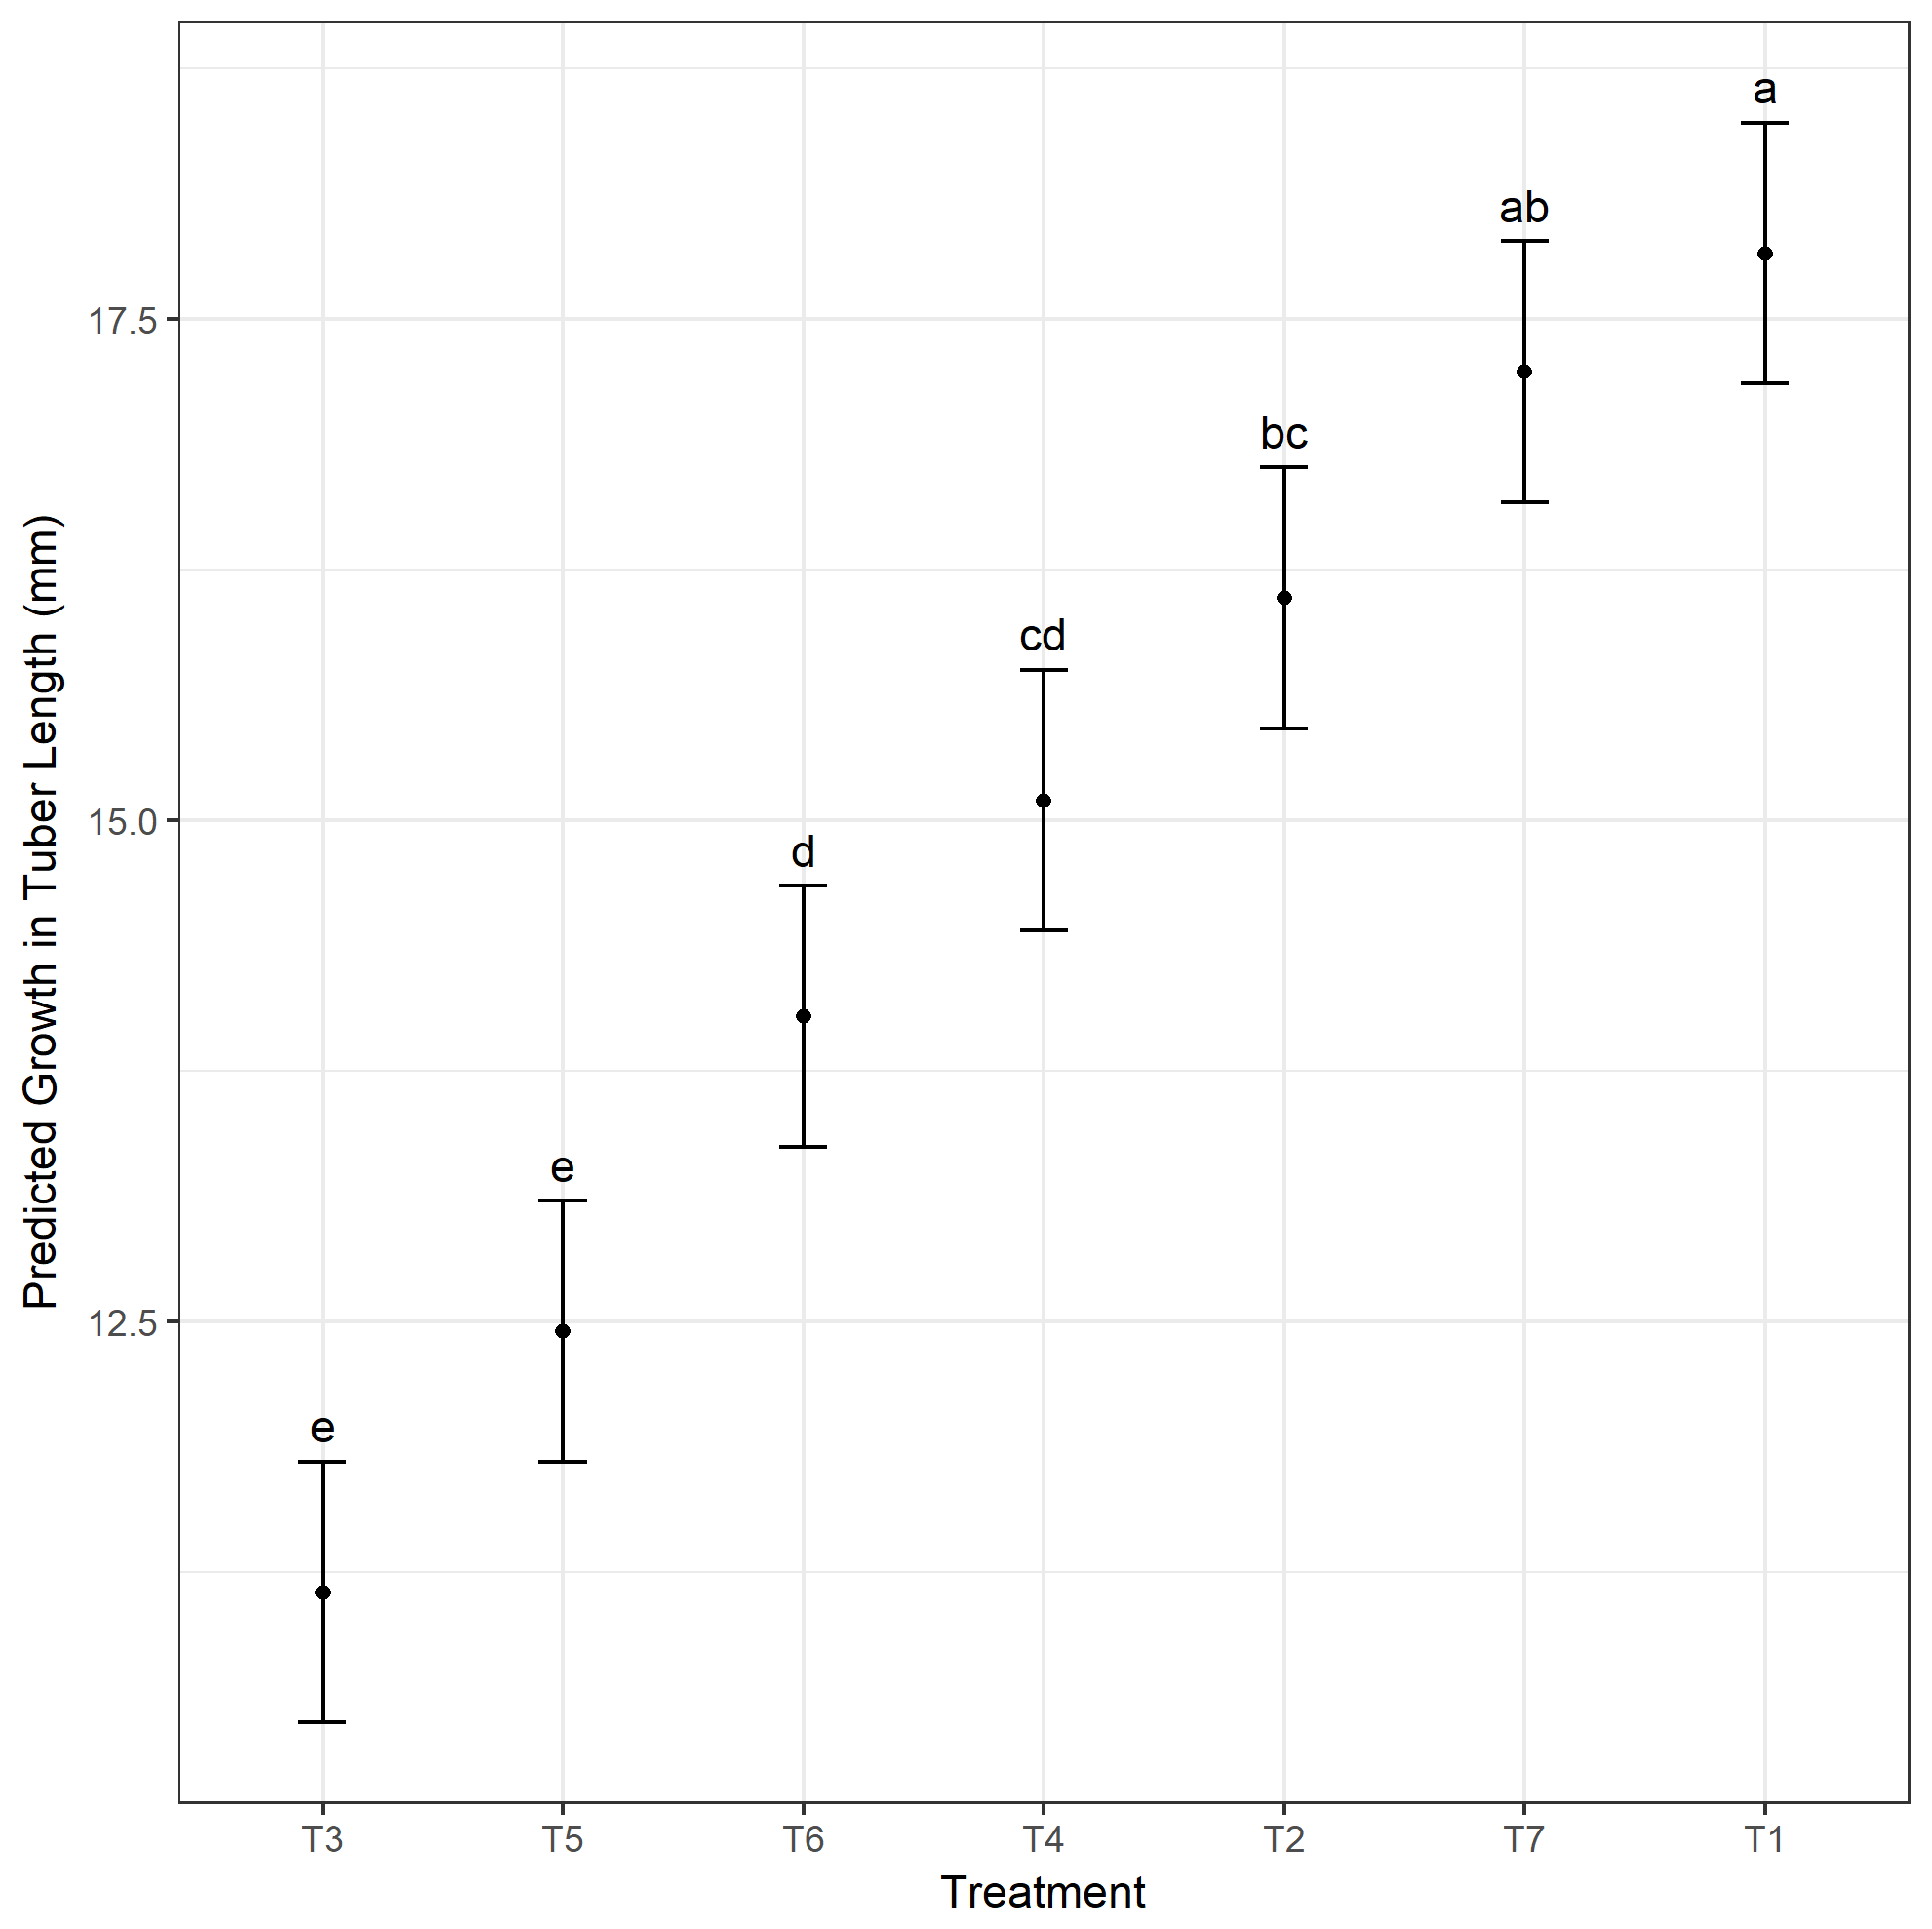
\includegraphics[width=0.8\textwidth, frame]{Example2Pred.png}
\end{tcolorbox}

\clearpage

\textbf{Exercise 1}

A  wheat variety trial run in Wagga in 2003 was designed using a completely randomised design. The aim of the
experiment was to determine if there were differences between the yields of the different varieties. The 12 varieties
were randomised to the plots in the field using a completely randomised design with three replicates. It was laid out
in the field in an array of plots 9 rows by 4 columns.

The 36 plots are the experimental and the observational units and the design layout is shown below:
\begin{center}
\small
\begin{tabular}{|l|c|c|c|c|}
  \hline
    & \textbf{Column 1} & \textbf{Column 2} & \textbf{Column 3} & \textbf{Column 4} \\
  \hline
  \textbf{Row 1} & Drysdale &  Pugsley & Baxter &  Zippy \\
  \hline
  \textbf{Row 2} & Caryina &  Zippy & Drysdale &  Janz \\
  \hline
  \textbf{Row 3} & Pugsley & Fortune &  Orion &  Caryina \\
  \hline
  \textbf{Row 4} & Lang &  Caryina &  Pugsley & Endure \\
  \hline
  \textbf{Row 5} & Endure &  Baxter &  Janz &  Lang \\
  \hline
  \textbf{Row 6} & Janz &  Wylah & Endure &  Orion \\
  \hline
  \textbf{Row 7} & Arrino &  Lang &  Fortune &  Wylah \\
  \hline
  \textbf{Row 8} & Fortune &  Drysdale &  Wylah & Arrino \\
  \hline
  \textbf{Row 9} & Baxter &  Arrino &  Zippy & Orion \\
  \hline
\end{tabular}\\
\end{center}

The data can be found in \texttt{exercise1.csv}. Import the data into R and analyse the data to determine whether
variety has an effect on yield. That is

\begin{align*}
& H_0: \mu_{Arrino} = \mu_{Baxter} = \hdots \ \mu_{Zippy} \: (\text{The variety means are equal})\\
& H_1: \texttt{not all } \mu_i \texttt{ are equal} \: (\text{Not all the variety means are equal})\\
\end{align*}

Carry out a complete analysis by:
\begin{enumerate}
  \item Graphing the data to determine whether the centres and the spread are the same or not.
  \item Fit the model to the data.
  \item Check the model assumptions.
  \item Interpret all the output.
  \item Predict the means and the standard errors from the model.
  \item If the variety factor is significant, carry out a Tukey's multiple comparison test and graph the results.
\end{enumerate}

\clearpage

\textbf{Exercise 2}

Seed priming has been successfully demonstrated to improve germination  and  emergence  in  seeds  of  many  crops, an
experiment was conducted to determine the effect of six different seed priming treatments on the time to germination
(days) on sunflower seeds. The six treatments were randomised to the plots in the field using a completely randomised
design with 4 replicates.  It was laid out in the field in an array of plots 8 rows by 3 columns.


The data can be found in \texttt{exercise2.csv}. Import the data into R and
analyse the data to determine whether treatment has an effect on time to
germination. That is

\begin{align*}
& H_0: \mu_{CN} = \mu_{CP} = \hdots \ \mu_{HE} \: (\text{The treatment means are equal})\\
& H_1: \texttt{not all } \mu_i \texttt{ are equal} \: (\text{Not all the treatment means are equal})\\
\end{align*}

Carry out a complete analysis by:
\begin{enumerate}
  \item Graphing the data to determine whether the centres and the spread are the same or not.
  \item Fit the model to the data.
  \item Check the model assumptions.
  \item Interpret all the output.
  \item Predict the means and the standard errors from the model.
  \item If the variety factor is significant, carry out a Tukey's multiple comparison test and graph the results.
\end{enumerate}

\clearpage



\section{Randomised Complete Block Design (RCBD)}

The randomised complete block design (RCBD) is the simplest design that includes blocking and is probably the most
frequently used design in research. In this design the number of experimental units in each block must equal the number
of treatments. Within each block, treatments are then randomly allocated within each block. As the design is carried
out taking into account the blocks, these are also fitted in the model when analysing the data.

From the design course we know that the skeletal ANOVA table for a RCBD looks like:

\begin{verbatim}
Source of Variation                      df
===================================================
Block stratum                            b-1
---------------------------------------------------
trt                                      t-1
Residual                                 (b-1)(t-1)
===================================================
Total                                    bt-1
\end{verbatim}

where $t$ are the number of treatments and $b$ is the number of blocks.

The total variance associated with the data is partitioned up into variance associated with the treatments, blocks and
residual.


\begin{figure}[!hbtp]
\centering
\fbox{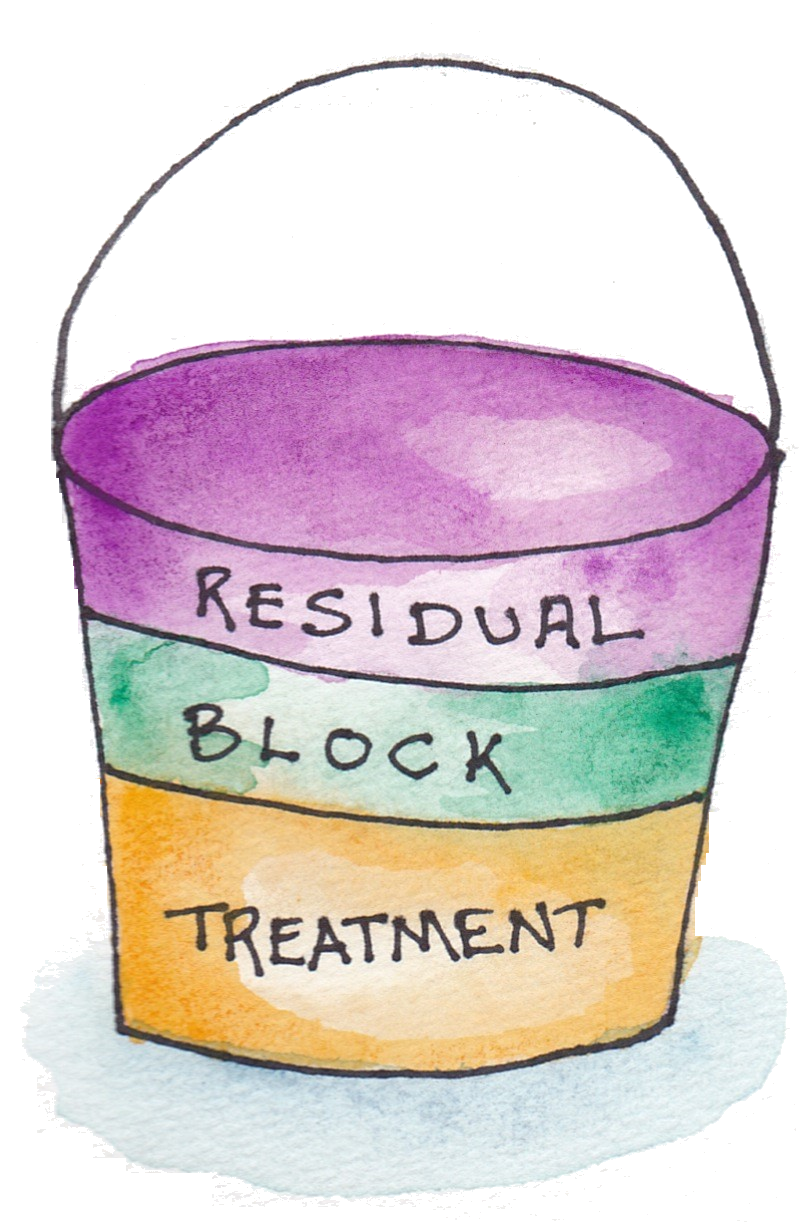
\includegraphics[width = 4cm]{rcbdbucket.png}}
\caption{Variance partitioning for a RCBD}
\label{fig:rcbdbucket}
\end{figure}

If Blocks are important (there is a difference between the blocks), the residual variation is reduced (as it is no
longer unexplained). As the hypothesis test concerning the treatments remains the same
($\frac{MS_{Trt}}{MS_{Residual}}$), treatment differences may be easier to detect. \clearpage

The analysis of variance table is formed as follows:

\footnotesize
\begin{tabular}{llllc}
\hline
   & & & &\\
  Source & SS & df & MS & F \\
   & & & &\\
  Treatment & $b \sum_{i=1}^{t} (\bar{y}_{i}-\bar{y})^2$ & $t-1$ & $\frac{SS_{Trt}}{t-1}$ & $\frac{MS_{Trt}}{MS_{Residual}}$ \\
   & & & &\\
  Block & $t \sum_{j=1}^{b} (\bar{y}_{j}-\bar{y})^2$ & $b-1$ & $\frac{SS_{Block}}{b-1}$ & \\
   & & & &\\
  Residual & $\sum_{i=1}^{t} \sum_{j=1}^{b} (\bar{y}_{ij}-\bar{y}_{i}-\bar{y}_{j} + \bar{y})^2$ & $(t-1)(b-1)$ & $\frac{SS_{Residual}}{(t-1)(b-1)}$ &  \\
   & & & &\\
   Total & $\sum_{i=1}^{t} \sum_{j=1}^{b} (\bar{y}_{ij}-\bar{y})^2 $ & $tb-1$ &  &  \\
   & & & &\\
  \hline
\end{tabular} \\
%\end{sidewaystable}
\normalsize

The main hypothesis of interest when analysing a randomised complete block design is the test for treatment effects.

\begin{eqnarray*}
H_0:& \texttt{all } \alpha_i = 0 \\
H_1:& \texttt{not all } \alpha_i \texttt{ are equal to zero} \\
\end{eqnarray*}\

or equivalently the test to determine whether the treatment means differ.

\begin{eqnarray*}
    H_0:& \texttt{all } \mu_i \texttt{ are equal} \\
    H_1:& \texttt{not all } \mu_i \texttt{ are equal} \\
\end{eqnarray*}\


The $F$ test statistic is given by:

\begin{eqnarray*}
F_{(t-1),(t-1)(b-1)} = \frac{MS_{Trt}}{MS_{Residual}}
\end{eqnarray*}


\clearpage
\textbf{Example 3}

A researcher wants to test for varietal differences between 4 varieties of field peas. Based on the information gained
during previous trials it was known that 5 replicates are required. The researcher used a randomised complete block
design, as there were known field trends that make using a randomised complete block a sensible option. The data can be
found in  \texttt{example3.csv}.


\begin{application}{Experiment Layout Sketch}
\vspace{10cm}
\end{application}


\begin{center}
\begin{tabular}{|c|c|c|c|c|c|}
  \hline
   & Col 1 & Col 2 & Col 3 & Col 4 & Col 5 \\
  \hline
  Row 1 & Parafield (0.45) & Yarrum (2.95) & Excell (6.28) & Kaspa (3.29) & Yarrum (8.20) \\
  \hline
  Row 2 & Yarrum (5.28) & Parafield (1.70) & Kaspa (0.30) & Yarrum (3.45) & Excell (5.14) \\
  \hline
  Row 3 & Excell (2.94) & Kaspa (1.94) & Parafield (1.69) & Parafield (0.04) & Kaspa (5.68) \\
  \hline
  Row 4 & Kaspa (2.17) & Excell (5.56) & Yarrum (3.74) & Excell (4.32) & Parafield (4.52) \\
  \hline
\end{tabular} \\
\end{center}
By inspection of this table we are able to confirm that a randomised complete block has been used and that the columns
form the blocks in this case. (Each column has a complete set of treatments.) The first part of this analysis will be
to graph the data to check the data integrity. The important aspects of this experiment are:

\begin{enumerate}
\item The null hypothesis is that all the varieties will have the same yield, that is:
\begin{align*}
& H_0: \texttt{The fieldpea yield is not dependent on the variety}\\
& H_1:\texttt{The fieldpea yield is dependent on the variety}\\
\end{align*}
\item A randomised complete block design has been used. \\
\item The treatments are the varieties.\\
\item The experimental unit is the plot, as the varieties have been randomised to the plots.\\
\item The observational unit is also the plot, as the whole plot was harvested to give the yield measurement.\\
\item The experiment was conducted in the field in a rectangular array of rows and columns.\\
\end{enumerate}


\subsection{Data Checking}
The code to create the boxplots is given below:

\tcbset {colback = code!10!white, colframe = code}
\begin{tcolorbox}[title = Import and graph the data]
\begin{verbatim}
dat <- read.csv("example3.csv")                                # import the data
dat$Block <- factor(dat$Block)          # convert the block variable to a factor

str(dat)
summary(dat)
\end{verbatim}
\tcblower
\begin{verbatim}
ggplot(data = dat, aes(x = Variety, y = Yield)) + geom_boxplot() +
theme_bw()

ggplot(data = dat, aes(x = Block, y = Yield)) + geom_boxplot() +
theme_bw()

\end{verbatim}
\end{tcolorbox}


\subsection{Linear Model}
The linear model that is fit can be symbolically written as:
\begin{eqnarray*}
	\texttt{Response variable}&:& \texttt{Yield} \\
	\texttt{Structural component}&:& \texttt{Block}\\
	\texttt{Explanatory component}&:& \texttt{Variety}\\
	\texttt{Residual}&:& \texttt{Assume independence}
\end{eqnarray*}


\tcbset {colback = outpt!25!white, colframe = outpt}
\begin{tcolorbox}[title = Example 3 Boxplots of Yield]
\includegraphics[width=0.8\textwidth, frame]{example3Var_boxplot.pdf}
\tcblower
\includegraphics[width=0.8\textwidth, frame]{example3Blk_boxplot.pdf}
\end{tcolorbox}


\subsection{Fitting the Model}

\tcbset {colback = code!10!white, colframe = code}
\begin{tcolorbox}[title = Fitting the linear model for a RCBD]
\begin{verbatim}
dat.aov <- aov(Yield ~ Block + Variety, data = dat)            # fitting the model
\end{verbatim}

\tcblower
\begin{verbatim}
par(mfrow = c(2, 2))
plot(dat.aov)
anova(dat.aov)
shapiro.test(dat.aov$residuals)
\end{verbatim}
\end{tcolorbox}

\tcbset {colback = outpt!25!white, colframe = outpt}
\begin{tcolorbox}[title = Example 3 Output]
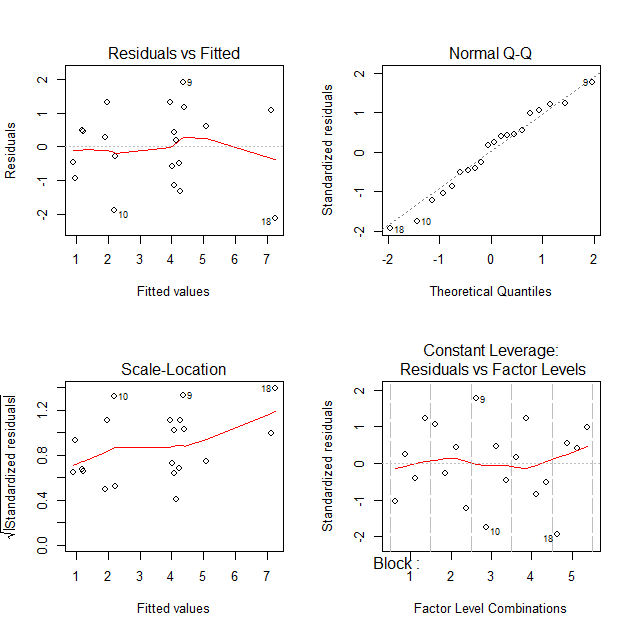
\includegraphics[width=0.8\textwidth, frame]{Example3Resplot.png}
\begin{verbatim}
Analysis of Variance Table

Response: Yield
          Df Sum Sq Mean Sq F value   Pr(>F)
Block      4 29.191  7.2977  3.7085 0.034525 *
Variety    3 36.527 12.1756  6.1873 0.008747 **
Residuals 12 23.614  1.9678
---
Signif. codes:  0 ‘***’ 0.001 ‘**’ 0.01 ‘*’ 0.05 ‘.’ 0.1 ‘ ’ 1
\end{verbatim}
\end{tcolorbox}

\clearpage
\subsection{Interpreting the Output}

The model assumptions need to be verified before the statistical inferences can be considered. Assumption 4 is assessed
using the first two graphs in the output (A and B) - the histogram and the QQ-plot. The histogram of the residuals
should be approximately symmetrical and bell-shaped, centred around zero. The QQ-plot displays the ordered residuals
plotted against the quantiles of the (in this case) Normal distribution. Deviations from the straight line indicates
deviation from the Normal distribution.

\tcbset {colback = interp!25!white, colframe = interp}
\begin{tcolorbox}[title = Example 3 Assumption 1]
\begin{verbatim}
When fitting an analysis of variance model as is done here Assumption 1
will always be true.
\end{verbatim}
\end{tcolorbox}


Assumption 2 is assessed using graph C - the residual plot. This plot should show approximately equal variance
(indicated by the vertical spread about zero) across the range of the fitted values.

\begin{tcolorbox}[title = Example 3 Assumption 2]
\begin{verbatim}
If the data have homogeneity of variances graph C should show
approximately equal variance across the range of the fitted values.

In this case the data show homogeneity of variances.
\end{verbatim}
\end{tcolorbox}

\begin{tcolorbox}[title = Example 3 Assumption 3]
\begin{verbatim}
Independence (Assumption 3) can safely be made given knowledge of the experimental
procedure. In this case we assume that the experiment was statistically designed
and run without complicating factors.
\end{verbatim}
\end{tcolorbox}

\begin{tcolorbox}[title = Example 3 Assumption 4]
\begin{verbatim}
Both the histogram and the QQ-plot show that the residuals follow an
approximate Normal distribution.

The Shapiro-Wilk test of normality is used to determine if the residuals
are normally distributed.
\end{verbatim}
\end{tcolorbox}

\tcbset {colback = outpt!25!white, colframe = outpt}
\begin{tcolorbox}[title = Example 3 Shapiro-Wilk normality test output]
\begin{verbatim}
        Shapiro-Wilk normality test

data:  dat.aov$residuals
W = 0.97153, p-value = 0.7868
\end{verbatim}
\end{tcolorbox}


\tcbset {colback = interp!25!white, colframe = interp}
\begin{tcolorbox}[title = Example 3 Shapiro-Wilk normality test interpretation]
\begin{verbatim}

In this case we can conclude that the residuals are derived from a population
that is normally distributed (as the Shapiro-Wilk p-value = 0.7868).

\end{verbatim}
\end{tcolorbox}



\begin{tcolorbox}[title = Example 3 Assumption 5]
\begin{verbatim}
It is assumed that the treatments are allocated without error.
\end{verbatim}
\end{tcolorbox}

The model assumptions are met - it is valid to consider the results in the analysis of variance table.

\tcbset {colback = interp!25!white, colframe = interp}
\begin{tcolorbox}[title = Example 3 ANOVA interpretation]
\begin{verbatim}

The p-value = 0.008747 is highly significant, and conclude there is
evidence to suggest that not all the variety means are the same. Less
importantly, there are also significant effects due to the Block variable,
p-value = 0.035.

\end{verbatim}
\end{tcolorbox}
\subsection{Prediction}

\tcbset {colback = code!10!white, colframe = code}
\begin{tcolorbox}[title = Example 3 predicted values]
\begin{verbatim}
library(emmeans)

pred.out <- emmeans(dat.aov, "Variety")
pred.out
pred.out <- data.frame(pred.out)

\end{verbatim}
\end{tcolorbox}

\tcbset {colback = outpt!25!white, colframe = outpt}
\begin{tcolorbox}[title = Example 3 Predicted output]
\begin{verbatim}
 Variety   emmean        SE df  lower.CL upper.CL
 Excell     4.848 0.6273483 12 3.4811256 6.214874
 Kaspa      2.676 0.6273483 12 1.3091256 4.042874
 Parafield  1.680 0.6273483 12 0.3131256 3.046874
 Yarrum     4.724 0.6273483 12 3.3571256 6.090874

Results are averaged over the levels of: Block
Confidence level used: 0.95

\end{verbatim}
\end{tcolorbox}

\tcbset {colback = interp!25!white, colframe = interp}
\begin{tcolorbox}[title = Example 3 Prediction interpretation]
\begin{lstlisting}
Parafield has the lowest predicted yield of 1.68t/ha ($\pm$ 0.627t/ha)
and Excell has the highest predicted yield of
4.85t/ha ($\pm$ 0.627t/ha).
\end{lstlisting}
\end{tcolorbox}

\clearpage
\subsection{Multiple Comparison Test}

\tcbset {colback = code!10!white, colframe = code}
\begin{tcolorbox}[title = Example 3 Tukey's multiple comparison]
\begin{verbatim}
tuk.out <- HSD.test(dat.aov, trt = "Variety", console = TRUE)
tuk.out$groups$Variety <- factor(row.names(tuk.out$groups))

pred.out <- left_join(pred.out, tuk.out$groups, by = "Variety")
pred.out
\end{verbatim}
\end{tcolorbox}


\tcbset {colback = outpt!25!white, colframe = outpt}
\begin{tcolorbox}[title = Example 3 Tukey's multiple comparison output]
\begin{verbatim}
Study: dat.aov ~ "Variety"

HSD Test for Yield

Mean Square Error:  1.967829

Variety,  means

          Yield      std r  Min  Max
Excell    4.848 1.280828 5 2.94 6.28
Kaspa     2.676 1.990234 5 0.30 5.68
Parafield 1.680 1.751328 5 0.04 4.52
Yarrum    4.724 2.128974 5 2.95 8.20

Alpha: 0.05 ; DF Error: 12
Critical Value of Studentized Range: 4.19866

Minimum Significant Difference: 2.634022

Treatments with the same letter are not significantly different.

          Yield groups
Excell    4.848      a
Yarrum    4.724      a
Kaspa     2.676     ab
Parafield 1.680      b

\end{verbatim}
\tcblower
\begin{verbatim}
    Variety emmean        SE df  lower.CL upper.CL Yield groups
1    Excell  4.848 0.6273483 12 3.4811256 6.214874 4.848      a
2     Kaspa  2.676 0.6273483 12 1.3091256 4.042874 2.676     ab
3 Parafield  1.680 0.6273483 12 0.3131256 3.046874 1.680      b
4    Yarrum  4.724 0.6273483 12 3.3571256 6.090874 4.724      a

\end{verbatim}
\end{tcolorbox}



\tcbset {colback = interp!25!white, colframe = interp}
\begin{tcolorbox}[title = Example 3 Prediction interpretation]
\begin{verbatim}
At the family 5% significance level:
- Excell and Yarrum are not significantly different (to each other)
but both are significantly higher than Parafield
- Kaspa is not significantly different from any of the other varieties
- Parafield is significantly lower than Excell and Yarrum
\end{verbatim}
\end{tcolorbox}




\tcbset {colback = code!10!white, colframe = code}
\begin{tcolorbox}[title = Example 3 Graph of predicted values]
\begin{verbatim}
# Calculate the upper and lower limits of the confidence intervals
pred.out$ci <-  qnorm(0.975)*pred.out$SE    #95% Confidence Interval
pred.out$low <- pred.out$emmean - pred.out$ci
pred.out$up <- pred.out$emmean + pred.out$ci

# order the Treatments by yield size
pred.out <- pred.out[order(pred.out$emmean),]
pred.out$Variety <- factor(as.character(pred.out$Variety),
                        levels = as.character(pred.out$Variety))
 
# graph the predicted values 
ggplot(data = pred.out, aes(x = Variety)) +
geom_errorbar(aes(ymin = low, ymax = up), width = 0.2) +
geom_text(aes(x = Variety, y = up, label = groups), vjust = 0, nudge_y = 0.05) +
geom_point(aes(y = emmean), color = "black", shape = 16) + theme_bw() +
labs(x = "Variety", y = "Predicted Yield (t/ha)")
\end{verbatim}
\end{tcolorbox}





\tcbset {colback = outpt!25!white, colframe = outpt}
\begin{tcolorbox}[title = Example 3 Graph of predicted values]
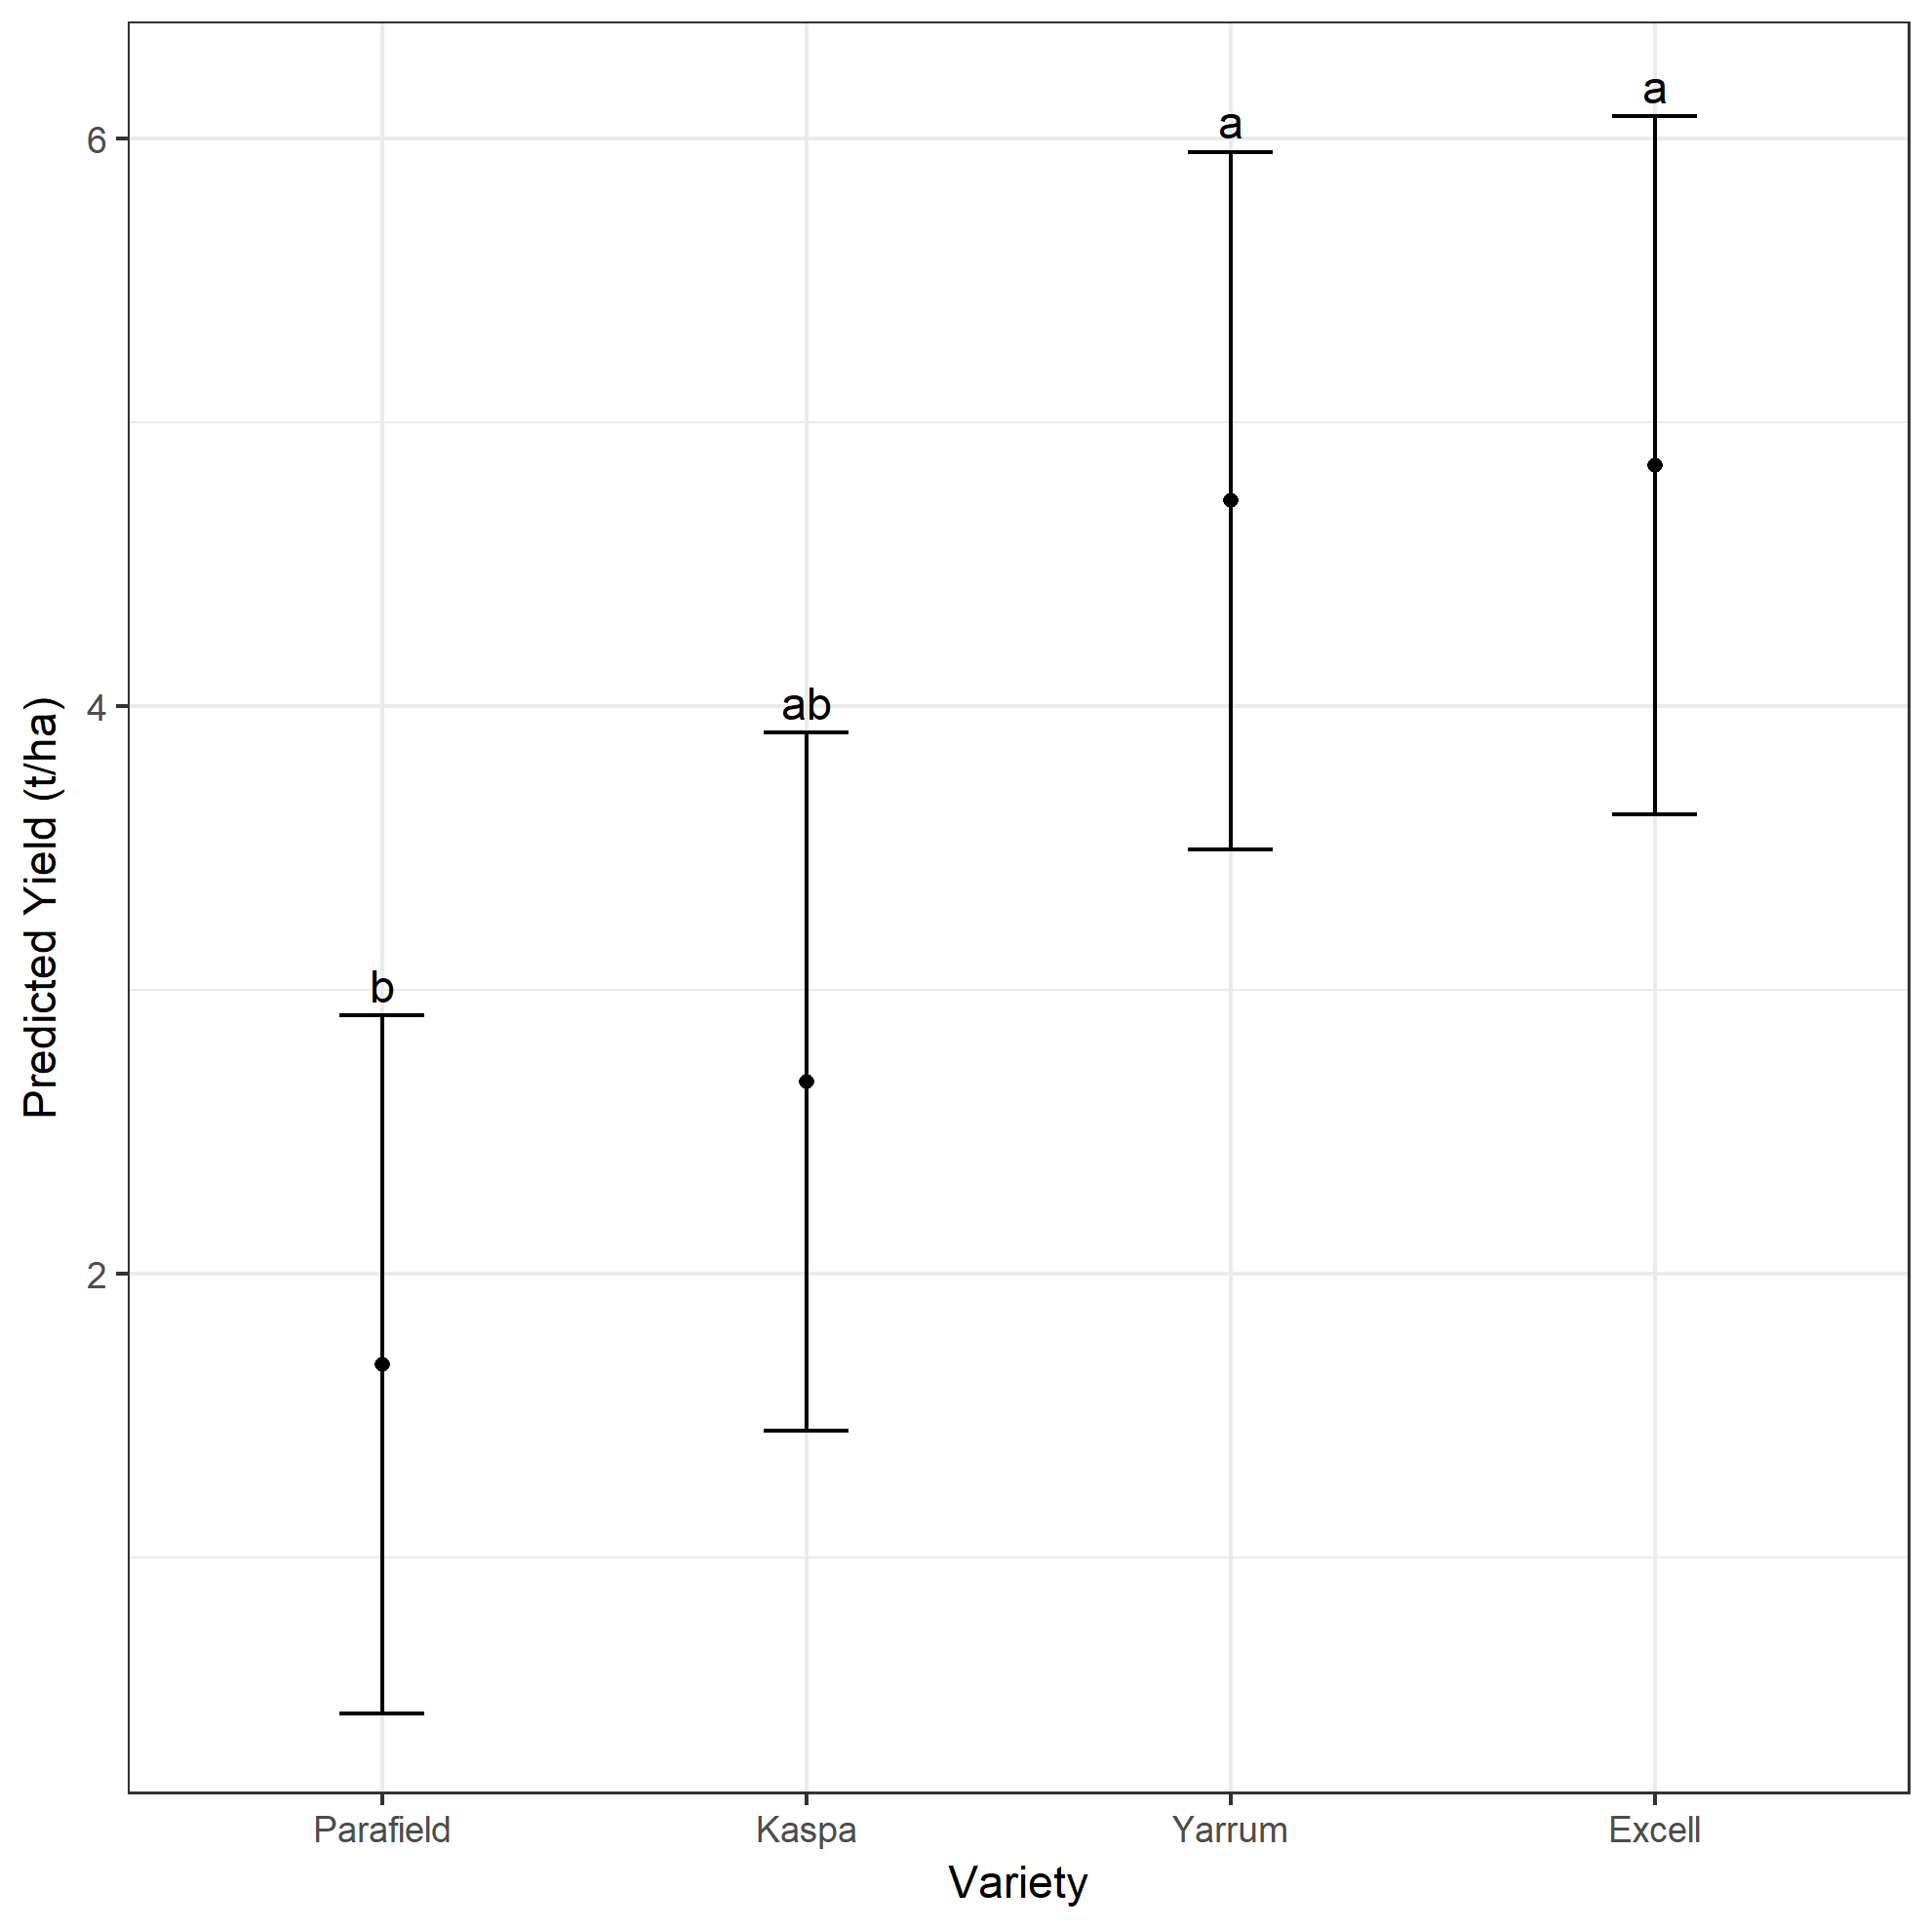
\includegraphics[width=0.8\textwidth, frame]{Example3Pred.png}
\end{tcolorbox}
\clearpage
\textbf{Exercise 3}

An experiment was conducted to assess the average fruit size (kg) in different watermelon varieties. A randomized
complete block layout was used where a complete set of varieties was randomised within a replicate which corresponded
to a row in the field. There were five replicates with seven varieties in each replicate. In the field the plots were
arranged in an array of 5 rows by 7 columns. The results can be found in \texttt{exercise3.csv}


Carry out a complete analysis by:
\begin{enumerate}
  \item Graphing the data to determine whether the centres and the spread are the same or not.
  \item Fit the model to the data.
  \item Check the model assumptions.
  \item Interpret all the output.
  \item Predict the means and the standard errors from the model.
  \item If the variety factor is significant, carry out a Tukey's multiple comparison test and graph the results.
\end{enumerate}


\textbf{Exercise 4}

An experiment was conducted to assess the yield (t/ha) of a single rice variety at various seeding rates (kg/ha) in a
field trial. A randomized complete block design based on six seeding rates with four blocks. In the field the plots
were arranged in an array of 6 rows by 4 columns. The results can be found in \texttt{exercise4.csv}


Carry out a complete analysis by:
\begin{enumerate}
  \item Graphing the data to determine whether the centres and the spread are the same or not.
  \item Fit the model to the data.
  \item Check the model assumptions.
  \item Interpret all the output.
  \item Predict the means and the standard errors from the model.
  \item If the seeding rate factor is significant, carry out a Tukey's multiple comparison test and graph the
      results.
\end{enumerate}

\clearpage


\section{Latin Square}

The Latin Square Design is where the number of rows and columns has to correspond to the number of treatment levels,
and therefore the number of replicates. The treatment allocation is done so that each treatment occurs once in each
column and row. As the design is carried out taking into account the rows and columns, these are also fitted in the
model when analysing the data.

From the design course we know that the skeletal ANOVA table for a LS looks like:

\begin{lstlisting}[mathescape=true]
Source of Variation                      df
============================================================
Row                                      (t-1)
Column                                   (t-1)
Treatment                                (t-1)
Residual                                 (t-1)(t-2)
============================================================
Total                                    (t$^2$ - 1)
\end{lstlisting}

where $t$ are the number of treatments.

The linear model that is fit can be symbolically written as:
\begin{eqnarray*}
	\texttt{Response variable}&:& \texttt{Yield} \\
	\texttt{Structural component}&:& \texttt{Row, Column}\\
	\texttt{Explanatory component}&:& \texttt{Variety}\\
	\texttt{Residual}&:& \texttt{Assume independence}
\end{eqnarray*}



The total variance associated with the data is partitioned up into variance associated with the treatments, rows,
columns and residual.


\begin{figure}[!hbtp]
\centering
\fbox{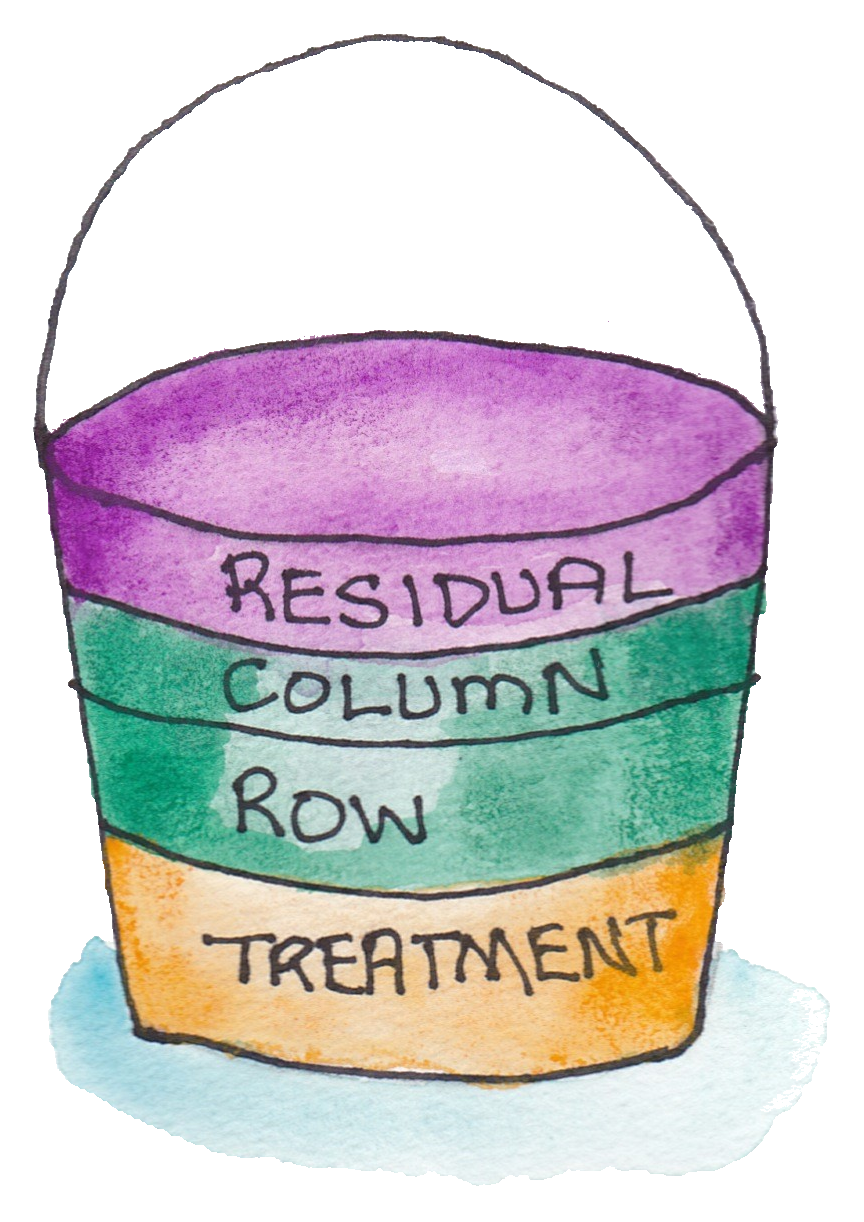
\includegraphics[width = 4cm]{lsbucket.png}}
\caption{Variance partitioning for a LS}
\label{fig:lsbucket}
\end{figure}

If Rows and/or Columns are important (there is a difference between the Rows and/or Columns), the residual variation is
reduced (as it is no longer unexplained). As the hypothesis test concerning the treatments remains the same
($\frac{MS_{Trt}}{MS_{Residual}}$), treatment differences may be easier to detect.

\clearpage

The analysis of variance table is formed as follows:

\footnotesize
\begin{tabular}{llllc}
\hline
   & & & &\\
  Source & SS & df & MS & F \\
   & & & &\\
  Row & $t \sum_{j=1}^{t} (\bar{y}_{j}-\bar{y})^2$ & $t-1$ & $\frac{SS_{Row}}{t-1}$ & \\
   & & & &\\
  Column & $t \sum_{k=1}^{t} (\bar{y}_{k}-\bar{y})^2$ & $t-1$ & $\frac{SS_{Column}}{t-1}$ & \\
   & & & &\\
  Treatment & $t \sum_{i=1}^{t} (\bar{y}_{i}-\bar{y})^2$ & $t-1$ & $\frac{SS_{Trt}}{t-1}$ & $\frac{MS_{Trt}}{MS_{Residual}}$ \\
   & & & &\\
  Residual & $ \sum_{j=1}^{t}\sum_{k=1}^{t} (\bar{y}_{ijk}-\bar{y}_{i}-\bar{y}_{j}-\bar{y}_{k} + 2\bar{y})^2$ & $(t-1)(t-2)$ & $\frac{SS_{Residual}}{(t-1)(t-2)}$ &  \\
   & & & &\\
   Total & $\sum_{i=1}^{t} \sum_{j=1}^{b} (\bar{y}_{ij}-\bar{y})^2 $ & $t^2-1$ &  &  \\
   & & & &\\
  \hline
\end{tabular} \\
%\end{sidewaystable}
\normalsize

The main hypothesis of interest when analysing a Latin square block design is the test for treatment effects.

\begin{eqnarray*}
H_0:& \texttt{all } \alpha_i = 0 \\
H_1:& \texttt{not all } \alpha_i \texttt{ are equal to zero} \\
\end{eqnarray*}\

or equivalently the test to determine whether the treatment means differ.

\begin{eqnarray*}
H_0:& \texttt{all } \mu_i \texttt{ are equal} \\
H_1:& \texttt{not all } \mu_i \texttt{ are equal} \\
\end{eqnarray*}\


The $F$ test statistic is given by:

\begin{eqnarray*}
F_{(t-1),(t-1)(b-1)} = \frac{MS_{Trt}}{MS_{Residual}}
\end{eqnarray*}

\textbf{Example 4}

An experiment was run to investigate the effects of four different soil type on the growth of lupins. The experiment was done with
pots on a bench in a glasshouse with systematic trend running along the bench (from left to right) as a result of the
temperature gradient, and across the bench (up and down) because of differing lighting levels. Due to this systematic
trend a LS design was used.


\begin{enumerate}
\item The null hypothesis is that all the soil types will have the same Dry Matter, that is:
\begin{align*}
& H_0: \texttt{The lupin dry matter is not dependent on the soil type}\\
& H_1:\texttt{The lupin dry matter is dependent on the soil type}\\
\end{align*}
\item A Latin square design has been used. \\
\item The treatments are the soil types.\\
\item The experimental unit is the pot, as the soil types have been randomised to the pots.\\
\item The observational unit is also the pot.\\
\item The experiment was conducted in the glasshouse in a rectangular array of rows and columns.\\
\end{enumerate}


\begin{application}{Experiment Layout Sketch}
\vspace{10cm}
\end{application}


\subsection{Data Checking}
The code to create the boxplots is given below:

\tcbset {colback = code!10!white, colframe = code}
\begin{tcolorbox}[title = Import and graph the data]
\begin{verbatim}
dat <- read.csv("example4.csv")               # import the data
dat$row <- factor(dat$row)
dat$col <- factor(dat$col)

str(dat)
summary(dat)
\end{verbatim}
\tcblower
\begin{verbatim}
ggplot(data = dat, aes(x = trt, y = DM)) + geom_boxplot() +
theme_bw()

ggplot(data = dat, aes(x = row, y = DM)) + geom_boxplot() +
theme_bw()

ggplot(data = dat, aes(x = col, y = DM)) + geom_boxplot() +
theme_bw()
\end{verbatim}
\end{tcolorbox}


\subsection{Linear Model}
The linear model that is fit can be symbolically written as:
\begin{eqnarray*}
	\texttt{Response variable}&:& \texttt{DM} \\
	\texttt{Structural component}&:& \texttt{row, column}\\
	\texttt{Explanatory component}&:& \texttt{Soil Type (trt)}\\
	\texttt{Residual}&:& \texttt{Assume independence}
\end{eqnarray*}


\tcbset {colback = outpt!25!white, colframe = outpt}
\begin{tcolorbox}[title = Example 4 Boxplots]
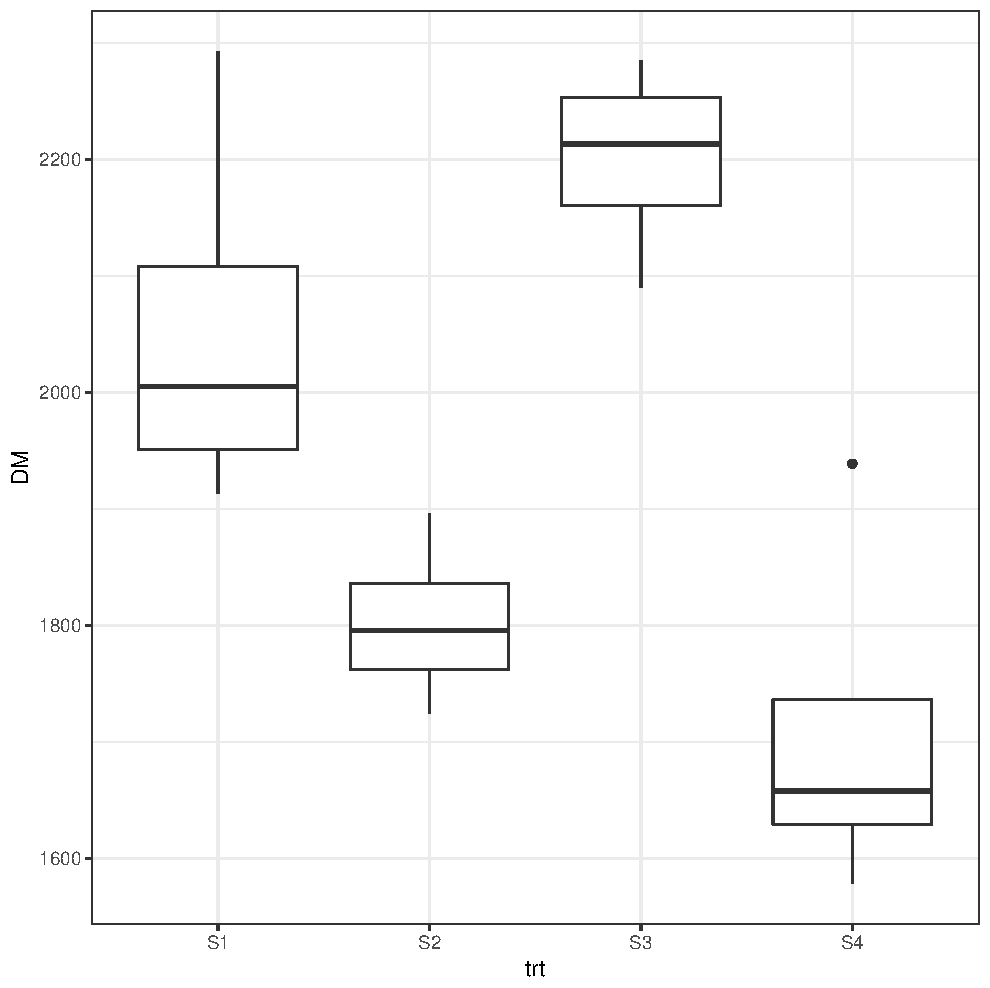
\includegraphics[width=0.5\textwidth, frame]{Example4trt_boxplot.pdf}
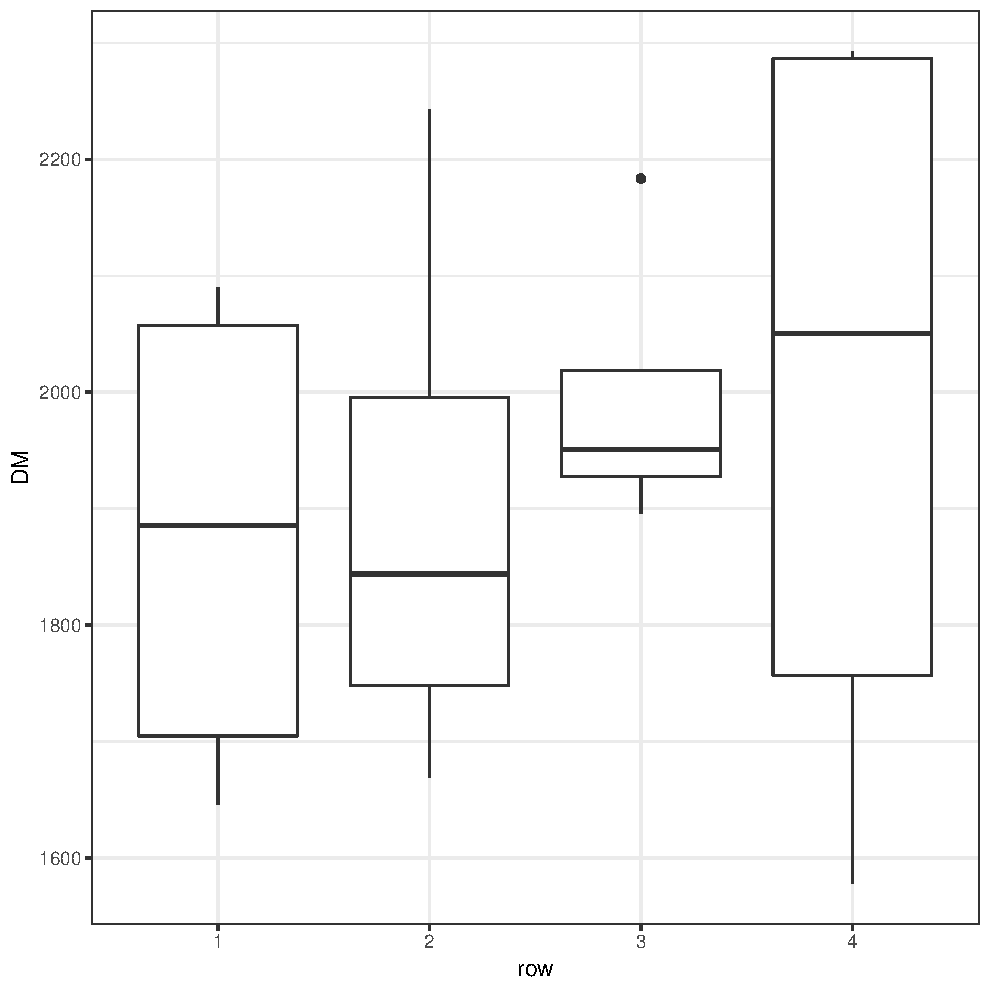
\includegraphics[width=0.5\textwidth, frame]{Example4row_boxplot.pdf}
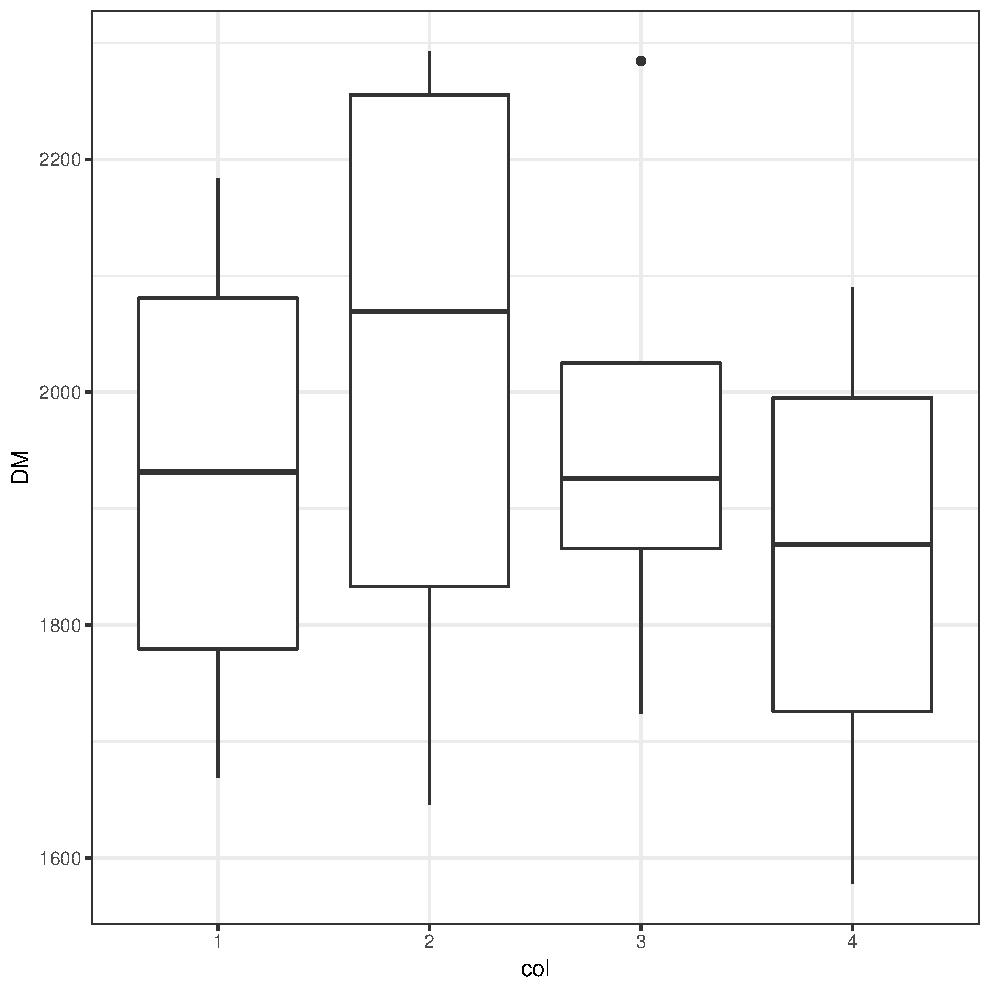
\includegraphics[width=0.5\textwidth, frame]{Example4col_boxplot.pdf}
\end{tcolorbox}


\subsection{Fitting the Model}

\tcbset {colback = code!10!white, colframe = code}
\begin{tcolorbox}[title = Fitting the linear model for a LS]
\begin{verbatim}
dat.aov <- aov(DM ~ row + col + trt, data = dat)
\end{verbatim}

\tcblower
\begin{verbatim}
par(mfrow = c(2, 2))
plot(dat.aov)
anova(dat.aov)
shapiro.test(dat.aov$residuals)
\end{verbatim}
\end{tcolorbox}

\tcbset {colback = outpt!25!white, colframe = outpt}
\begin{tcolorbox}[title = Example 4 Output]
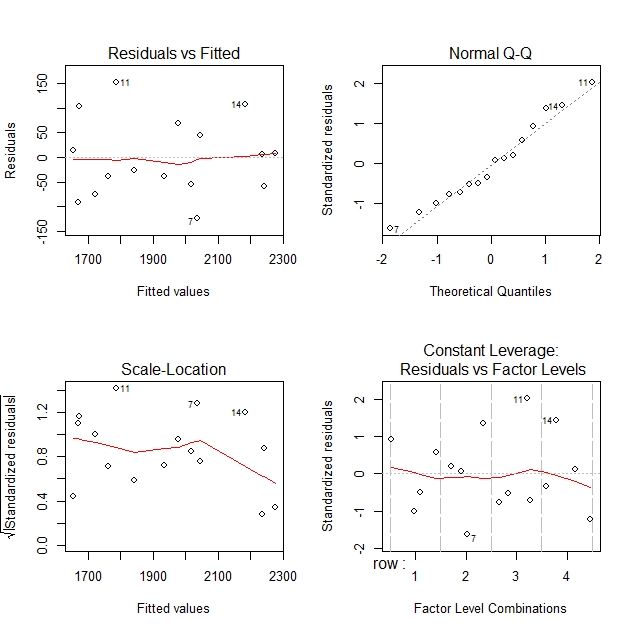
\includegraphics[width=0.8\textwidth, frame]{Example4Resplot.png}
\begin{verbatim}
Analysis of Variance Table

Response: DM
          Df Sum Sq Mean Sq F value   Pr(>F)
row        3  45760   15253  0.9928 0.457425
col        3  59232   19744  1.2851 0.361855
trt        3 613113  204371 13.3020 0.004638 **
Residuals  6  92184   15364
---
Signif. codes:  0 ‘***’ 0.001 ‘**’ 0.01 ‘*’ 0.05 ‘.’ 0.1 ‘ ’ 1
\end{verbatim}
\end{tcolorbox}


\subsection{Interpreting the Output}

The model assumptions need to be verified before the statistical inferences can be considered. Assumption 4 is assessed
using the first two graphs in the output (A and B) - the histogram and the QQ-plot. The histogram of the residuals
should be approximately symmetrical and bell-shaped, centred around zero. The QQ-plot displays the ordered residuals
plotted against the quantiles of the (in this case) Normal distribution. Deviations from the straight line indicates
deviation from the Normal distribution.

\tcbset {colback = interp!25!white, colframe = interp}
\begin{tcolorbox}[title = Example 4 Assumption 1]
\begin{verbatim}
When fitting an analysis of variance model as is done here
Assumption 1 will always be true.
\end{verbatim}
\end{tcolorbox}


Assumption 2 is assessed using graph C - the residual plot. This plot should show approximately equal variance
(indicated by the vertical spread about zero) across the range of the fitted values.

\begin{tcolorbox}[title = Example 4 Assumption 2]
\begin{verbatim}
If the data have homogeneity of variances graph C should show
approximately equal variance across the range of the fitted values.

In this case the data show homogeneity of variances.
\end{verbatim}
\end{tcolorbox}

\begin{tcolorbox}[title = Example 4 Assumption 3]
\begin{verbatim}
Independence (Assumption 3) can safely be made given knowledge of the experimental
procedure. In this case we assume that the experiment was statistically designed
and run without complicating factors.
\end{verbatim}
\end{tcolorbox}

\begin{tcolorbox}[title = Example 4 Assumption 4]
\begin{verbatim}
Both the histogram and the QQ-plot show that the residuals follow an
approximate Normal distribution.

The Shapiro-Wilk test of normality is used to determine if the residuals
are normally distributed.
\end{verbatim}
\end{tcolorbox}

\tcbset {colback = outpt!25!white, colframe = outpt}
\begin{tcolorbox}[title = Example 4 Shapiro-Wilk normality test output]
\begin{verbatim}
        Shapiro-Wilk normality test

data:  dat.aov$residuals
W = 0.96553, p-value = 0.762
\end{verbatim}
\end{tcolorbox}


\tcbset {colback = interp!25!white, colframe = interp}
\begin{tcolorbox}[title = Example 4 Shapiro-Wilk normality test interpretation]
\begin{verbatim}

In this case we can conclude that the residuals are derived from a population
that is normally distributed (as the Shapiro-Wilk p-value = 0.762).

\end{verbatim}
\end{tcolorbox}



\begin{tcolorbox}[title = Example 4 Assumption 5]
\begin{verbatim}
It is assumed that the treatments are allocated without error.
\end{verbatim}
\end{tcolorbox}

The model assumptions are met - it is valid to consider the results in the analysis of variance table.

\tcbset {colback = interp!25!white, colframe = interp}
\begin{tcolorbox}[title = Example 4 ANOVA interpretation]
\begin{verbatim}

The p-value = 0.004638 is highly significant, and conclude there is
evidence to suggest that not all the soil type means are the same.
\end{verbatim}
\end{tcolorbox}
\subsection{Prediction}

\tcbset {colback = code!10!white, colframe = code}
\begin{tcolorbox}[title = Example 4 predicted values]
\begin{verbatim}
library(emmeans)
pred.out <- emmeans(dat.aov, "trt")
pred.out
pred.out <- data.frame(pred.out)
\end{verbatim}
\end{tcolorbox}

\tcbset {colback = outpt!25!white, colframe = outpt}
\begin{tcolorbox}[title = Example 4 Predicted output]
\begin{verbatim}
 trt   emmean       SE df lower.CL upper.CL
 S1  2053.733 61.97568  6 1902.083 2205.382
 S2  1802.697 61.97568  6 1651.048 1954.347
 S3  2200.085 61.97568  6 2048.436 2351.734
 S4  1707.940 61.97568  6 1556.291 1859.589

Results are averaged over the levels of: row, col
Confidence level used: 0.95
\end{verbatim}
\end{tcolorbox}

\tcbset {colback = interp!25!white, colframe = interp}
\begin{tcolorbox}[title = Example 4 Prediction interpretation]
\begin{lstlisting}
S4 has the lowest predicted DM of 1708kg/ha ($\pm$ 62.0kg/ha)
and S3 has the highest predicted DM of 2200kg/ha
($\pm$62.0kg/ha).
\end{lstlisting}
\end{tcolorbox}


\subsection{Multiple Comparison Test}

\tcbset {colback = code!10!white, colframe = code}
\begin{tcolorbox}[title = Example 4 Tukey's multiple comparison]
\begin{verbatim}
tuk.out <- HSD.test(dat.aov, trt = "trt", console = TRUE)
tuk.out$groups$trt <- factor(row.names(tuk.out$groups))

pred.out <- left_join(pred.out, tuk.out$groups, by = "trt")
pred.out
\end{verbatim}
\end{tcolorbox}
\clearpage


\tcbset {colback = outpt!25!white, colframe = outpt}
\begin{tcolorbox}[title = Example 4 Tukey's multiple comparison output]
\begin{verbatim}
Study: dat.aov ~ "trt"

HSD Test for DM

Mean Square Error:  15363.94

trt,  means

         DM       std r     Min     Max
S1 2053.733 168.16724 4 1912.96 2292.06
S2 1802.697  72.44064 4 1724.18 1895.56
S3 2200.085  84.31568 4 2089.97 2284.36
S4 1707.940 158.39339 4 1578.44 1938.45

Alpha: 0.05 ; DF Error: 6
Critical Value of Studentized Range: 4.895599

Minimum Significant Difference: 303.4081

Treatments with the same letter are not significantly different.

         DM groups
S3 2200.085      a
S1 2053.733     ab
S2 1802.697     bc
S4 1707.940      c
\end{verbatim}
\tcblower
\begin{verbatim}
  trt   emmean       SE df lower.CL upper.CL       DM groups
1  S1 2053.733 61.97568  6 1902.083 2205.382 2053.733     ab
2  S2 1802.697 61.97568  6 1651.048 1954.347 1802.697     bc
3  S3 2200.085 61.97568  6 2048.436 2351.734 2200.085      a
4  S4 1707.940 61.97568  6 1556.291 1859.589 1707.940      c
\end{verbatim}
\end{tcolorbox}

\tcbset {colback = interp!25!white, colframe = interp}
\begin{tcolorbox}[title = Example 4 Prediction interpretation]
\begin{verbatim}
At the family 5% significance level:
- S1 and S4 are significantly different
- S2 and S3 are significantly different
- S3 is not significantly different to S1 but significantly different
      from both S2 or S4
- S4 is not significantly different to S2 but significantly different
      from S3
\end{verbatim}
\end{tcolorbox}
\tcbset {colback = code!10!white, colframe = code}
\begin{tcolorbox}[title = Example 4 Graph of predicted values]
\begin{verbatim}
# Calculate the upper and lower limits of the confidence intervals
pred.out$ci <-  qnorm(0.975)*pred.out$SE    #95% Confidence Interval
pred.out$low <- pred.out$emmean - pred.out$ci
pred.out$up <- pred.out$emmean + pred.out$ci

# order the Treatments by AverageFruitSize size
pred.out <- pred.out[order(pred.out$emmean),]
pred.out$trt <- factor(as.character(pred.out$trt),
                                levels = as.character(pred.out$trt))
 
# graph the predicted values 
ggplot(data = pred.out, aes(x = trt)) +
geom_errorbar(aes(ymin = low, ymax = up), width = 0.2) +
geom_text(aes(x = trt, y = up, label = groups), vjust = 0, nudge_y = 5) +
geom_point(aes(y = emmean), color = "black", shape = 16) + theme_bw() +
labs(x = "Soil Type", y = "Predicted Dry Matter (kg/ha)")
\end{verbatim}
\end{tcolorbox}


\tcbset {colback = outpt!25!white, colframe = outpt}
\begin{tcolorbox}[title = Example 4 Graph of predicted values]
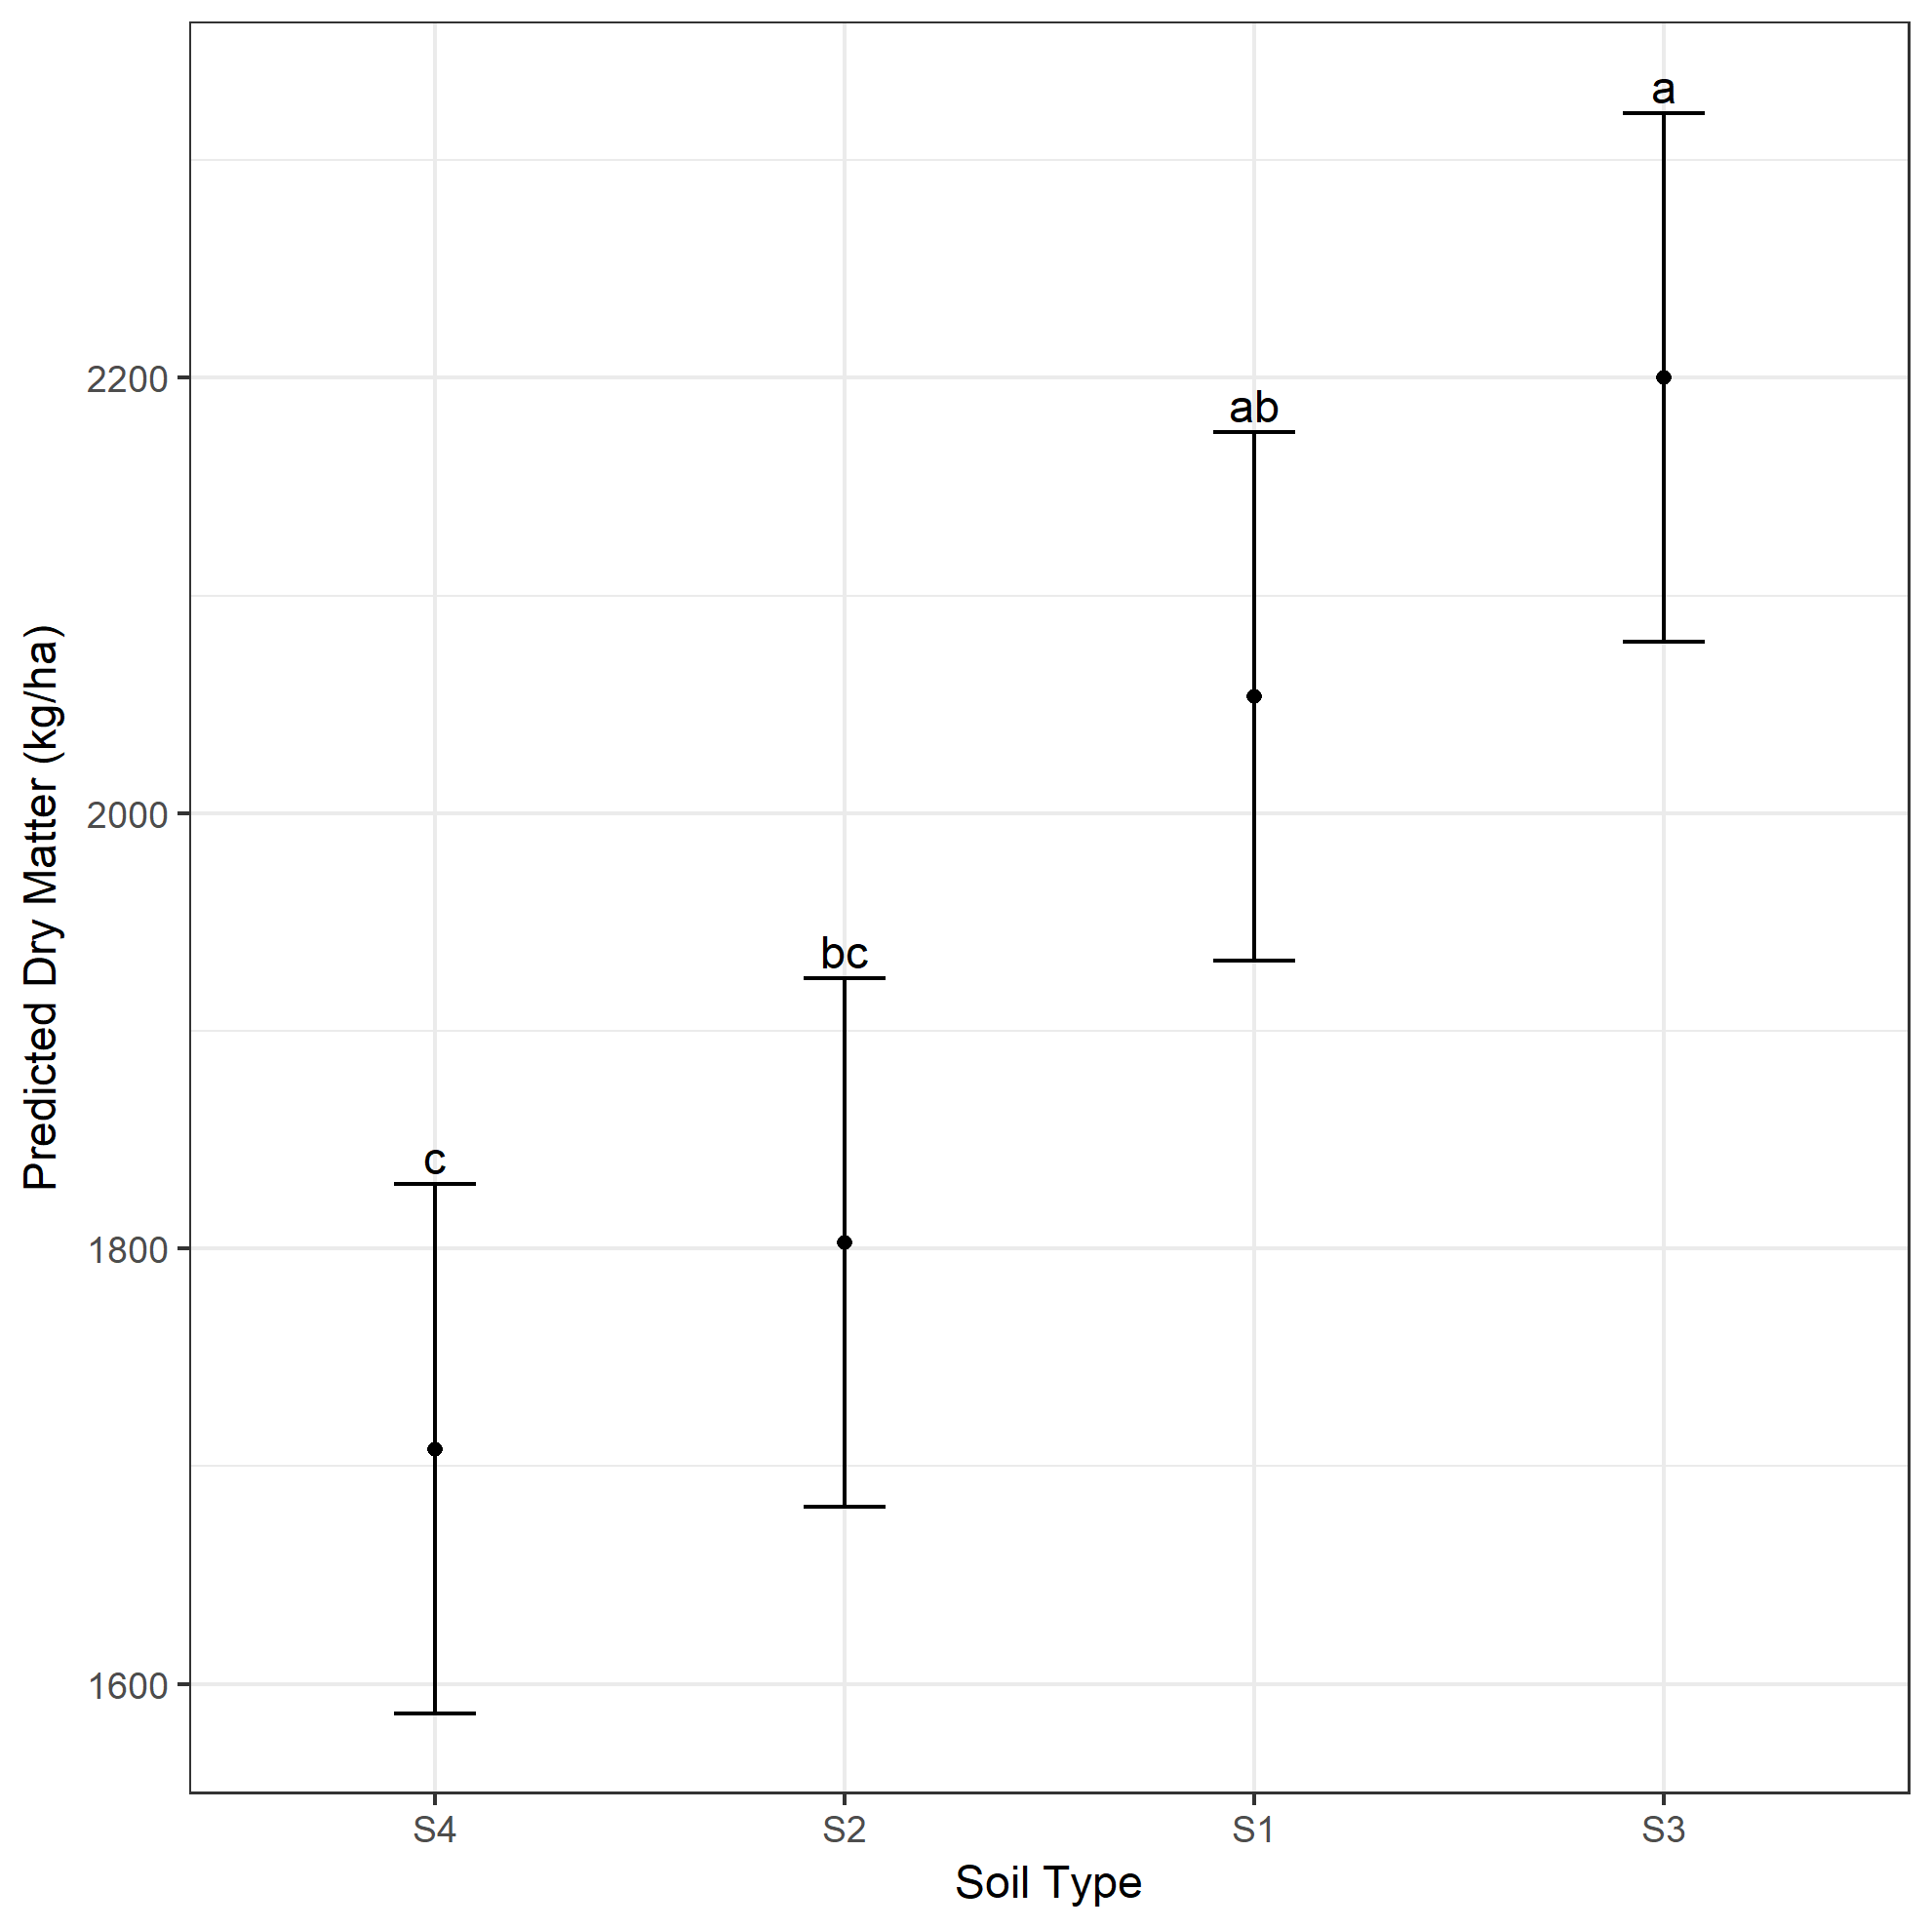
\includegraphics[width=0.8\textwidth, frame]{Example4Pred.png}
\end{tcolorbox}
\clearpage


\textbf{Exercise 5}

A pilot experiment was conducted to investigate the pathogen of Ear Rot in Maize. A Latin Square design was used with
five pathways of the pathogen into the plant, seed, stalks, silks, roots and plant damage. The researchers wanted to
determine the effect of the pathway on the percentage infection evident in the ear of the maize. The results can be
found in \texttt{exercise5.csv}


Carry out a complete analysis by:
\begin{enumerate}
  \item Graphing the data to determine whether the centres and the spread are the same or not.
  \item Fit the model to the data.
  \item Check the model assumptions.
  \item Interpret all the output.
  \item Predict the means and the standard errors from the model.
  \item If the pathogen pathway factor is significant, carry out a Tukey's multiple comparison test and graph the
      results.
\end{enumerate}


\textbf{Exercise 6}

Nutgrass management is an important issue affecting productivity and profitability in sugarcane production in
Australia. Studies have shown the capacity of nutgrass to compete with crops if left uncontrolled. An experiment was
conducted to determine the effect of the control of nutgrass on the sugar yield  (t/ha) of sugar cane. The trial design
was a Latin square design with four treatments:
\begin{enumerate}
\item T0 no nutgrass competition
\item T4 nutgrass controlled after 4 weeks competition
\item T8 nutgrass controlled after 8 weeks competition
\item T12 nutgrass controlled after 12 weeks competition
\end{enumerate}
The results can be found in \texttt{exercise6.csv}


Carry out a complete analysis by:
\begin{enumerate}
  \item Graphing the data to determine whether the centres and the spread are the same or not.
  \item Fit the model to the data.
  \item Check the model assumptions.
  \item Interpret all the output.
  \item Predict the means and the standard errors from the model.
  \item If the treatment factor is significant, carry out a Tukey's multiple comparison test and graph the results.
\end{enumerate}

\clearpage


\chapter{Linear mixed models - Analysis of Variance}

In the previous chapter a linear model was used to analyse data arising from CR, RCB and LS designs and in R \cite{r}
the \texttt{aov} function was used to carry out this analysis. The results were reliant on the model assumptions being
met and in all examples investigated this was the case. In research often there is data that do not meet these
requirements, or that are not complete, or arise from more complex experiments. These data can be analysed using Linear
Mixed Models (LMM) using much the same process as previously used.

LMM's can be used instead of linear models, the mathematics behind the model is
quite different to a linear model but the results will be equivalent. A LMM
combines two models into one, a \textbf{fixed model} and a \textbf{random
model}. The fixed is used to describe the explanatory structure of the
experiment and the random is used to describe the structural component of the
experiment. Also, using a LMM the assumption of independence required for
linear models can be relaxed, as dependence can be modelled using LMM's.

In the first part of this chapter some of the previous examples will be revisited and analysed using a LMM approach.
ASReml-R \cite{asremlr} is used as the tool to analyse the data using the function \texttt{asreml}.

\section{LMM - introduction}

\textbf{Example 3}

The data can be found in  \texttt{example3.csv}.

\subsection{Linear Mixed Model}
The linear mixed model that is fit can be symbolically written as:
\begin{eqnarray*}
	\texttt{Response variable}&:& \texttt{Yield} \\
	\texttt{Structural component}&:& \texttt{Block}\\
	\texttt{Explanatory component}&:& \texttt{Variety}\\
	\texttt{Residual}&:& \texttt{Assume independence}
\end{eqnarray*}

As the data checking etc has already been completed it will not be repeated here, but would normally be the first part
of the analysis.

\subsection{Fitting the Model}

\tcbset {colback = code!10!white, colframe = code}
\begin{tcolorbox}[title = Fitting the linear mixed model for a RCBD]
\begin{verbatim}
library{asreml}
dat$Plot <- factor(dat$Plot)

dat.asr <- asreml(Yield ~ Variety, random = ~ Block,
                residual = ~ id(Plot), data = dat)
dat.ww <- wald(dat.asr, denDF = "default")$Wald
\end{verbatim}

\tcblower
\begin{verbatim}
plot(dat.asr)

#The ANOVA table
round(dat.ww,3)
shapiro.test(dat.asr$residuals)
\end{verbatim}
\end{tcolorbox}

\tcbset {colback = outpt!25!white, colframe = outpt}
\begin{tcolorbox}[title = Example 3 Output]
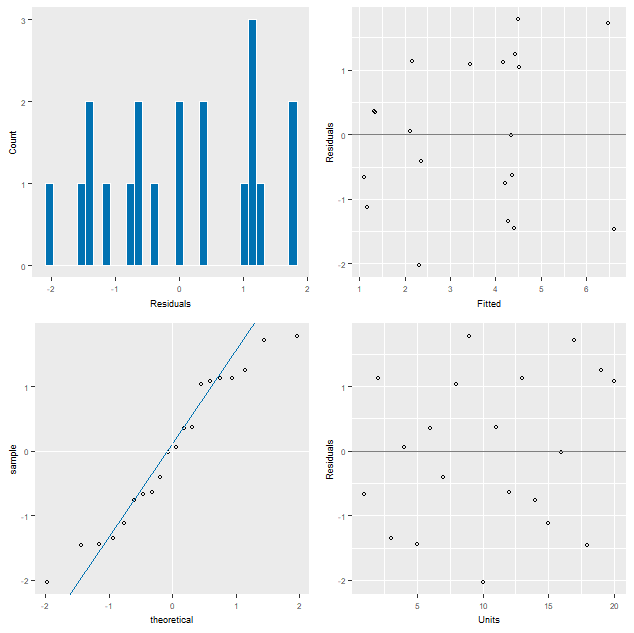
\includegraphics[width=0.8\textwidth, frame]{Example3LMMResplot.png}
\begin{verbatim}
            Df denDF  F.inc    Pr
(Intercept)  1     4 33.230 0.004
Variety      3    12  6.187 0.009
\end{verbatim}
\end{tcolorbox}


\subsection{Interpreting the Output}

The model assumptions need to be verified before the statistical inferences can be considered. The model assumptions
for a LMM are exactly the same as seen previously. Assumption 4 is assessed using the first two graphs in the output (A
and B) - the histogram and the QQ-plot. The histogram of the residuals should be approximately symmetrical and
bell-shaped, centred around zero. The QQ-plot displays the ordered residuals plotted against the quantiles of the (in
this case) Normal distribution. Deviations from the straight line indicates deviation from the Normal distribution.

\tcbset {colback = interp!25!white, colframe = interp}
\begin{tcolorbox}[title = Example 3 Assumption 1]
\begin{verbatim}
When fitting an analysis of variance model as is done here Assumption 1
will always be true.
\end{verbatim}
\end{tcolorbox}


Assumption 2 is assessed using graph C - the residual plot. This plot should show approximately equal variance
(indicated by the vertical spread about zero) across the range of the fitted values.

\begin{tcolorbox}[title = Example 3 Assumption 2]
\begin{verbatim}
If the data have homogeneity of variances graph C should show
approximately equal variance across the range of the fitted values.

In this case the data show homogeneity of variances.
\end{verbatim}
\end{tcolorbox}

\begin{tcolorbox}[title = Example 3 Assumption 3]
\begin{verbatim}
Independence (Assumption 3) can safely be made given knowledge of the experimental
procedure. In this case we assume that the experiment was statistically designed
and run without complicating factors.
\end{verbatim}
\end{tcolorbox}

\begin{tcolorbox}[title = Example 3 Assumption 4]
\begin{verbatim}
Both the histogram and the QQ-plot show that the residuals follow an
approximate Normal distribution.

The Shapiro-Wilk test of normality is used to determine if the residuals
are normally distributed.
\end{verbatim}
\end{tcolorbox}

\tcbset {colback = outpt!25!white, colframe = outpt}
\begin{tcolorbox}[title = Example 3 Shapiro-Wilk normality test output]
\begin{verbatim}
       Shapiro-Wilk normality test

data:  dat.asr$residuals
W = 0.94567, p-value = 0.306
\end{verbatim}
\end{tcolorbox}


\tcbset {colback = interp!25!white, colframe = interp}
\begin{tcolorbox}[title = Example 3 Shapiro-Wilk normality test interpretation]
\begin{verbatim}

In this case we can conclude that the residuals are derived from a population
that is normally distributed (as the Shapiro-Wilk p-value = 0.306).

\end{verbatim}
\end{tcolorbox}



\begin{tcolorbox}[title = Example 3 Assumption 5]
\begin{verbatim}
It is assumed that the Varieties are allocated without error.
\end{verbatim}
\end{tcolorbox}

The model assumptions are met - it is valid to consider the results in the analysis of variance table.

\tcbset {colback = interp!25!white, colframe = interp}
\begin{tcolorbox}[title = Example 3 ANOVA interpretation]
\begin{verbatim}

The p-value = 0.009 is highly significant, and conclude there is
evidence to suggest that not all the variety means are the same.
\end{verbatim}
\end{tcolorbox}
\subsection{Prediction}

\tcbset {colback = code!10!white, colframe = code}
\begin{tcolorbox}[title = Example 3 predicted values]
\begin{verbatim}
dat.pred <- predict(dat.asr, classify = "Variety",
sed = TRUE)
\end{verbatim}
\end{tcolorbox}

\tcbset {colback = outpt!25!white, colframe = outpt}
\begin{tcolorbox}[title = Example 3 Predicted output]
\begin{verbatim}
$pvals

Notes:
- The predictions are obtained by averaging across the hypertable
  calculated from model terms constructed solely from factors in
  the averaging and classify sets.
- Use 'average' to move ignored factors into the averaging set.
- The ignored set: Block


    Variety predicted.value std.error    status
1    Excell           4.848 0.8124417 Estimable
2     Kaspa           2.676 0.8124417 Estimable
3 Parafield           1.680 0.8124417 Estimable
4    Yarrum           4.724 0.8124417 Estimable

$sed
4 x 4 Matrix of class "dspMatrix"
          [,1]      [,2]      [,3]      [,4]
[1,]        NA 0.8872044 0.8872044 0.8872044
[2,] 0.8872044        NA 0.8872044 0.8872044
[3,] 0.8872044 0.8872044        NA 0.8872044
[4,] 0.8872044 0.8872044 0.8872044        NA

$avsed
      min      mean       max
0.8872044 0.8872044 0.8872044
\end{verbatim}
\end{tcolorbox}

\tcbset {colback = interp!25!white, colframe = interp}
\begin{tcolorbox}[title = Example 3 Prediction interpretation]
\begin{lstlisting}
Parafield has the lowest predicted yield of 1.68t/ha ($\pm$ 0.812t/ha) and
Excell has the highest predicted yield of
4.85t/ha ($\pm$ 0.812t/ha).
\end{lstlisting}
\end{tcolorbox}

\clearpage
\subsection{Multiple Comparison Test}

\tcbset {colback = code!10!white, colframe = code}
\begin{tcolorbox}[title = Example 3 Tukey's multiple comparison]
\begin{verbatim}
pred.out <- tuk.out(model.obj = dat.asr, pred.obj = dat.pred,
                    pred = "Variety", sig = 0.95)
\end{verbatim}
\end{tcolorbox}



\tcbset {colback = outpt!25!white, colframe = outpt}
\begin{tcolorbox}[title = Example 3 Tukey's multiple comparison output]
\begin{verbatim}
  predicted.value   Variety std.error    status groups       ci         low       up
1           1.680 Parafield 0.8124417 Estimable      a 1.722299 -0.04229944 3.402299
2           2.676     Kaspa 0.8124417 Estimable     ab 1.722299  0.95370056 4.398299
3           4.724    Yarrum 0.8124417 Estimable      b 1.722299  3.00170056 6.446299
4           4.848    Excell 0.8124417 Estimable      b 1.722299  3.12570056 6.570299
\end{verbatim}
\end{tcolorbox}

\tcbset {colback = interp!25!white, colframe = interp}
\begin{tcolorbox}[title = Example 3 Prediction interpretation]
\begin{verbatim}
At the family 5% significance level:
- Excell and Yarrum are not significantly different (to each other)
but both are significantly higher than Parafield
- Kaspa is not significantly different from any of the other varieties
- Parafield is significantly lower than Excell and Yarrum
\end{verbatim}
\end{tcolorbox}
\tcbset {colback = code!10!white, colframe = code}
\begin{tcolorbox}[title = Example 3 Graph of predicted values]
\begin{verbatim}
# order the Treatments by Yield size
pred.out <- pred.out[order(pred.out$predicted.value),]
pred.out$Variety <- factor(as.character(pred.out$Variety),
            levels = as.character(pred.out$Variety))

# graph the predicted values 
ggplot(data = pred.out, aes(x = Variety)) +
geom_errorbar(aes(ymin = low, ymax = up), width = 0.2) +
geom_text(aes(x = Variety, y = up, label = groups), vjust = 0, nudge_y = 0.2) +
geom_point(aes(y = predicted.value), color = "black", shape = 16) + theme_bw() +
labs(x = "", y = "Predicted Yield (t/ha)")
\end{verbatim}
\end{tcolorbox}


\tcbset {colback = outpt!25!white, colframe = outpt}
\begin{tcolorbox}[title = Example 3 Graph of predicted values]
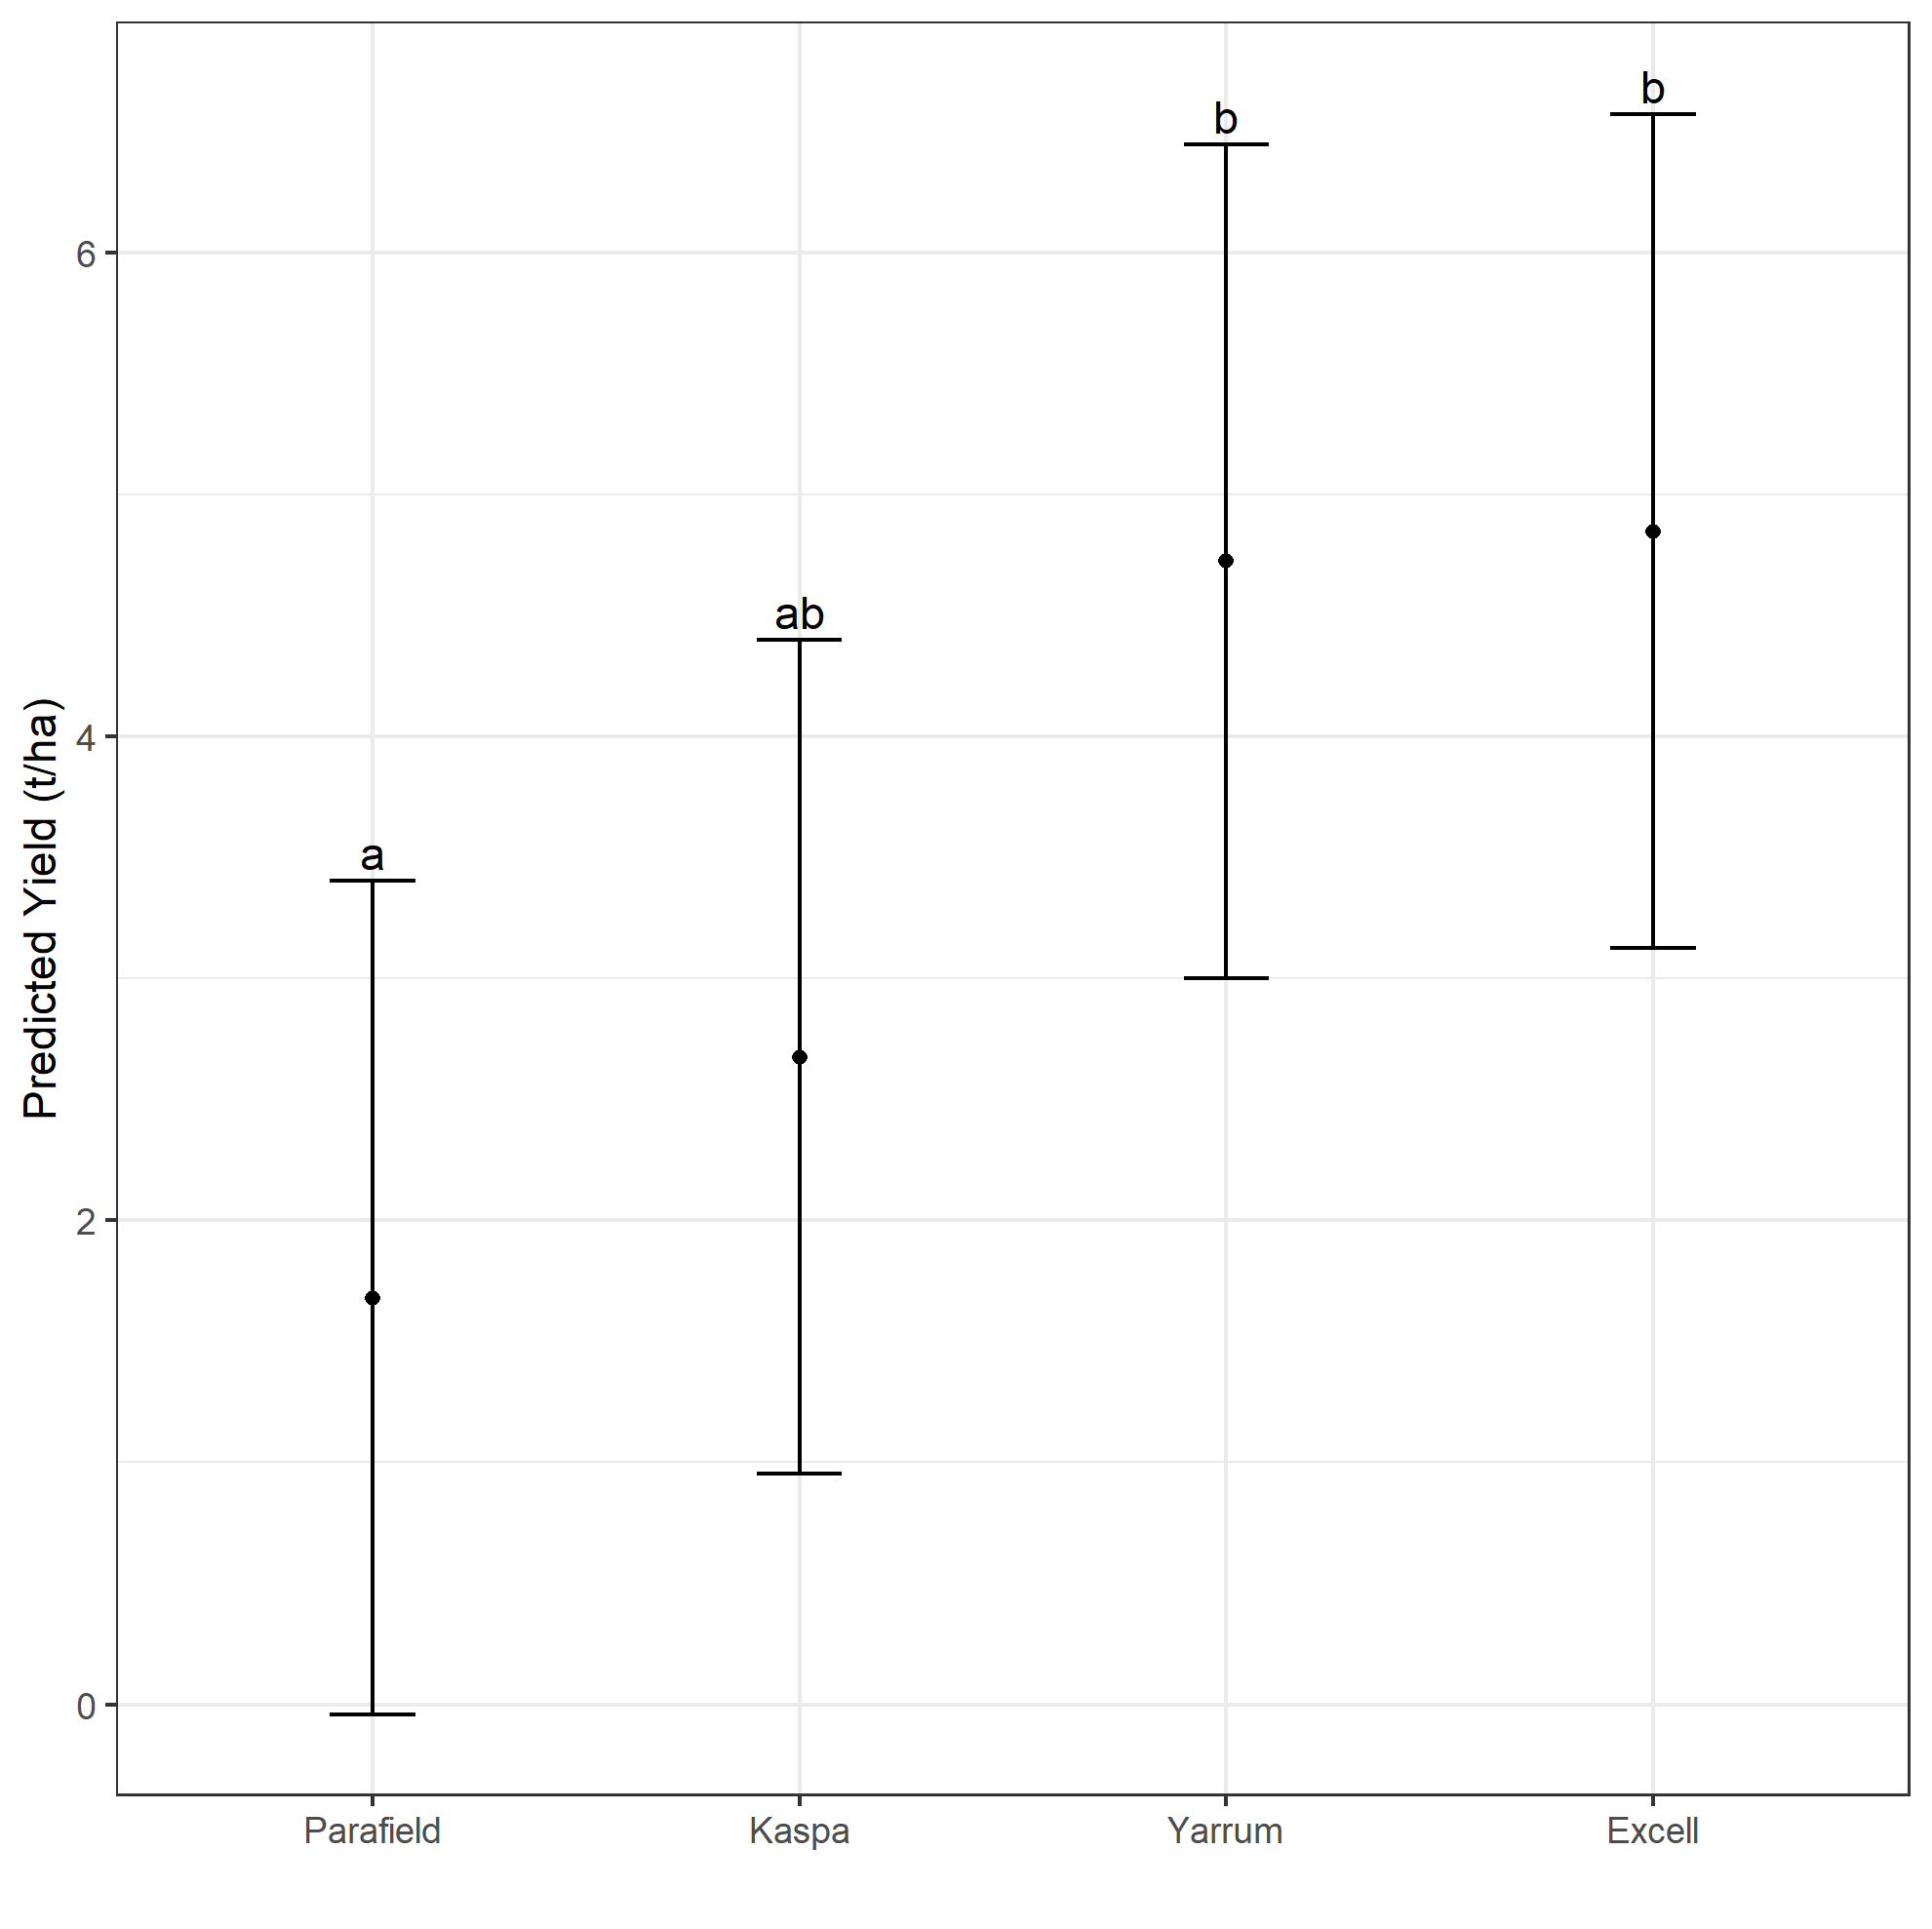
\includegraphics[width=0.8\textwidth, frame]{Example3LMMPred.png}
\end{tcolorbox}

\clearpage
\textbf{Example 4}

The data can be found in  \texttt{example4.csv}.

\subsection{Linear Mixed Model}
The linear mixed model that is fit can be symbolically written as:
\begin{eqnarray*}
	\texttt{Response variable}&:& \texttt{DM} \\
	\texttt{Structural component}&:& \texttt{row, column}\\
	\texttt{Explanatory component}&:& \texttt{Soil Type (trt)}\\
	\texttt{Residual}&:& \texttt{Assume independence}
\end{eqnarray*}

As the data checking etc has already been completed it will not be repeated here, but would normally be the first part
of the analysis.

\subsection{Fitting the Model}

\tcbset {colback = code!10!white, colframe = code}
\begin{tcolorbox}[title = Fitting the linear mixed model for a LS]
\begin{verbatim}
dat$plots <- factor(dat$plots)

dat.asr <- asreml(DM ~ trt, random = ~ row + col,
residual = ~ id(plots), data = dat)
dat.ww <- wald(dat.asr, denDF = "default")$Wald
\end{verbatim}

\tcblower
\begin{verbatim}
plot(dat.asr)
anova(dat.asr)
shapiro.test(dat.asr$residuals)
\end{verbatim}
\end{tcolorbox}
\clearpage \tcbset {colback = outpt!25!white, colframe = outpt}
\begin{tcolorbox}[title = Example 4 Output]
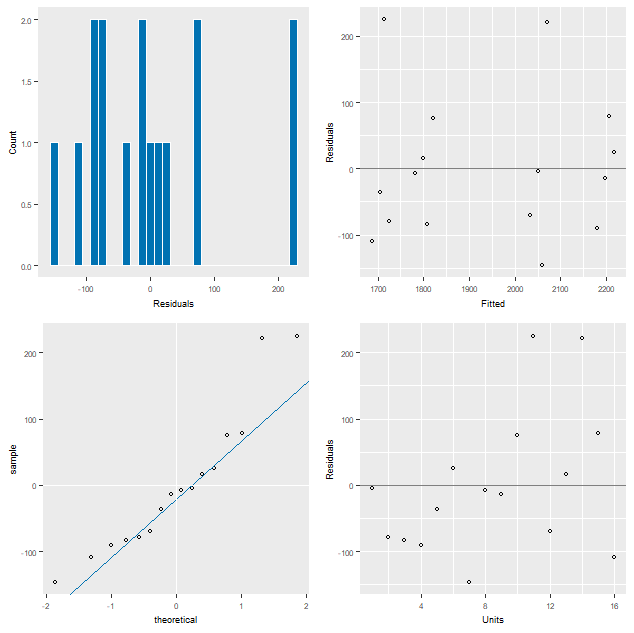
\includegraphics[width=0.8\textwidth, frame]{Example4LMMResplot.png}
\begin{verbatim}
            Df denDF   F.inc    Pr
(Intercept)  1     3 3053.00 0.000
trt          3     9   13.33 0.001
\end{verbatim}
\end{tcolorbox}


\subsection{Interpreting the Output}

The model assumptions need to be verified before the statistical inferences can be considered. Assumption 4 is assessed
using the first two graphs in the output (A and B) - the histogram and the QQ-plot. The histogram of the residuals
should be approximately symmetrical and bell-shaped, centred around zero. The QQ-plot displays the ordered residuals
plotted against the quantiles of the (in this case) Normal distribution. Deviations from the straight line indicates
deviation from the Normal distribution.

\tcbset {colback = interp!25!white, colframe = interp}
\begin{tcolorbox}[title = Example 4 Assumption 1]
\begin{verbatim}
When fitting an analysis of variance model as is done here
Assumption 1 will always be true.
\end{verbatim}
\end{tcolorbox}


Assumption 2 is assessed using graph C - the residual plot. This plot should show approximately equal variance
(indicated by the vertical spread about zero) across the range of the fitted values.

\begin{tcolorbox}[title = Example 4 Assumption 2]
\begin{verbatim}
If the data have homogeneity of variances graph C should show
approximately equal variance across the range of the fitted values.

In this case the data show homogeneity of variances.
\end{verbatim}
\end{tcolorbox}

\begin{tcolorbox}[title = Example 4 Assumption 3]
\begin{verbatim}
Independence (Assumption 3) can safely be made given knowledge of the experimental
procedure. In this case we assume that the experiment was statistically designed
and run without complicating factors.
\end{verbatim}
\end{tcolorbox}

\begin{tcolorbox}[title = Example 4 Assumption 4]
\begin{verbatim}
Both the histogram and the QQ-plot show that the residuals follow an
approximate Normal distribution.

The Shapiro-Wilk test of normality is used to determine if the residuals
are normally distributed.
\end{verbatim}
\end{tcolorbox}

\tcbset {colback = outpt!25!white, colframe = outpt}
\begin{tcolorbox}[title = Example 4 Shapiro-Wilk normality test output]
\begin{verbatim}
        Shapiro-Wilk normality test

data:  dat.asr$residuals
W = 0.9023, p-value = 0.0875
\end{verbatim}
\end{tcolorbox}


\tcbset {colback = interp!25!white, colframe = interp}
\begin{tcolorbox}[title = Example 4 Shapiro-Wilk normality test interpretation]
\begin{verbatim}

In this case we can conclude that the residuals are derived from a population
that is normally distributed (as the Shapiro-Wilk p-value = 0.0875).

\end{verbatim}
\end{tcolorbox}



\begin{tcolorbox}[title = Example 4 Assumption 5]
\begin{verbatim}
It is assumed that the treatments are allocated without error.
\end{verbatim}
\end{tcolorbox}

The model assumptions are met - it is valid to consider the results in the analysis of variance table.

\tcbset {colback = interp!25!white, colframe = interp}
\begin{tcolorbox}[title = Example 4 ANOVA interpretation]
\begin{verbatim}
The p-value = 0.001 is highly significant, and conclude there is
evidence to suggest that not all the soil type means are the same.
\end{verbatim}
\end{tcolorbox}
\subsection{Prediction}

\tcbset {colback = code!10!white, colframe = code}
\begin{tcolorbox}[title = Example 4 predicted values]
\begin{verbatim}
dat.pred <- predict(dat.asr, classify = "trt",
sed = TRUE)
\end{verbatim}
\end{tcolorbox}

\tcbset {colback = outpt!25!white, colframe = outpt}
\begin{tcolorbox}[title = Example 4 Predicted output]
\begin{verbatim}
$pvals

Notes:
- The predictions are obtained by averaging across the hypertable
  calculated from model terms constructed solely from factors in
  the averaging and classify sets.
- Use 'average' to move ignored factors into the averaging set.
- The ignored set: row,col


  trt predicted.value std.error    status
1  S1        2053.733  64.09245 Estimable
2  S2        1802.697  64.09245 Estimable
3  S3        2200.085  64.09245 Estimable
4  S4        1707.940  64.09245 Estimable

$sed
4 x 4 Matrix of class "dspMatrix"
        [,1]    [,2]    [,3]    [,4]
[1,]      NA 87.5417 87.5417 87.5417
[2,] 87.5417      NA 87.5417 87.5417
[3,] 87.5417 87.5417      NA 87.5417
[4,] 87.5417 87.5417 87.5417      NA

$avsed
    min    mean     max
87.5417 87.5417 87.5417
\end{verbatim}
\end{tcolorbox}

\tcbset {colback = interp!25!white, colframe = interp}
\begin{tcolorbox}[title = Example 4 Prediction interpretation]
\begin{lstlisting}
S4 has the lowest predicted DM of 1708kg/ha ($\pm$ 64.0kg/ha)
and S3 has the highest predicted DM of 2200kg/ha
($\pm$64.0kg/ha).
\end{lstlisting}
\end{tcolorbox}%%
\subsection{Multiple Comparison Test}

\tcbset {colback = code!10!white, colframe = code}
\begin{tcolorbox}[title = Example 4 Tukey's multiple comparison]
\begin{verbatim}
pred.out <- tuk.out(model.obj = dat.asr, pred.obj = dat.pred,
                            pred = "trt", sig = 0.95)
pred.out
\end{verbatim}
\end{tcolorbox}

\tcbset {colback = outpt!25!white, colframe = outpt}
\begin{tcolorbox}[title = Example 4 Tukey's multiple comparison output]
\begin{verbatim}
  predicted.value trt std.error groups       ci      low       up
1        1707.940  S4  64.09245      a 139.6454 1568.295 1847.585
2        1802.697  S2  64.09245     ab 139.6454 1663.052 1942.343
3        2053.733  S1  64.09245     bc 139.6454 1914.087 2193.378
4        2200.085  S3  64.09245      c 139.6454 2060.440 2339.730

\end{verbatim}
\end{tcolorbox}

\tcbset {colback = interp!25!white, colframe = interp}
\begin{tcolorbox}[title = Example 4 Prediction interpretation]
\begin{verbatim}
At the family 5% significance level:
- S1 and S4 are significantly different
- S2 and S3 are significantly different
- S3 is not significantly different to S1 but significantly different
      from both S2 or S4
- S4 is not significantly different to S2 but significantly different
      from S3
\end{verbatim}
\end{tcolorbox}


\tcbset {colback = code!10!white, colframe = code}
\begin{tcolorbox}[title = Example 4 Graph of predicted values]
\begin{verbatim}
# order the Treatments by DM
pred.out <- pred.out[order(pred.out$predicted.value),]
pred.out$trt <- factor(as.character(pred.out$trt),
                        levels = as.character(pred.out$trt))


# graph the predicted values 
ggplot(data = pred.out, aes(x = trt)) +
geom_errorbar(aes(ymin = low, ymax = up), width = 0.2) +
geom_text(aes(x = trt, y = up, label = groups), vjust = 0, nudge_y = 5) +
geom_point(aes(y = predicted.value), color = "black", shape = 16) + theme_bw() +
labs(x = "Soil Type", y = "Predicted Dry Matter (kg/ha)")

\end{verbatim}
\end{tcolorbox}


\tcbset {colback = outpt!25!white, colframe = outpt}
\begin{tcolorbox}[title = Example 4 Graph of predicted values]
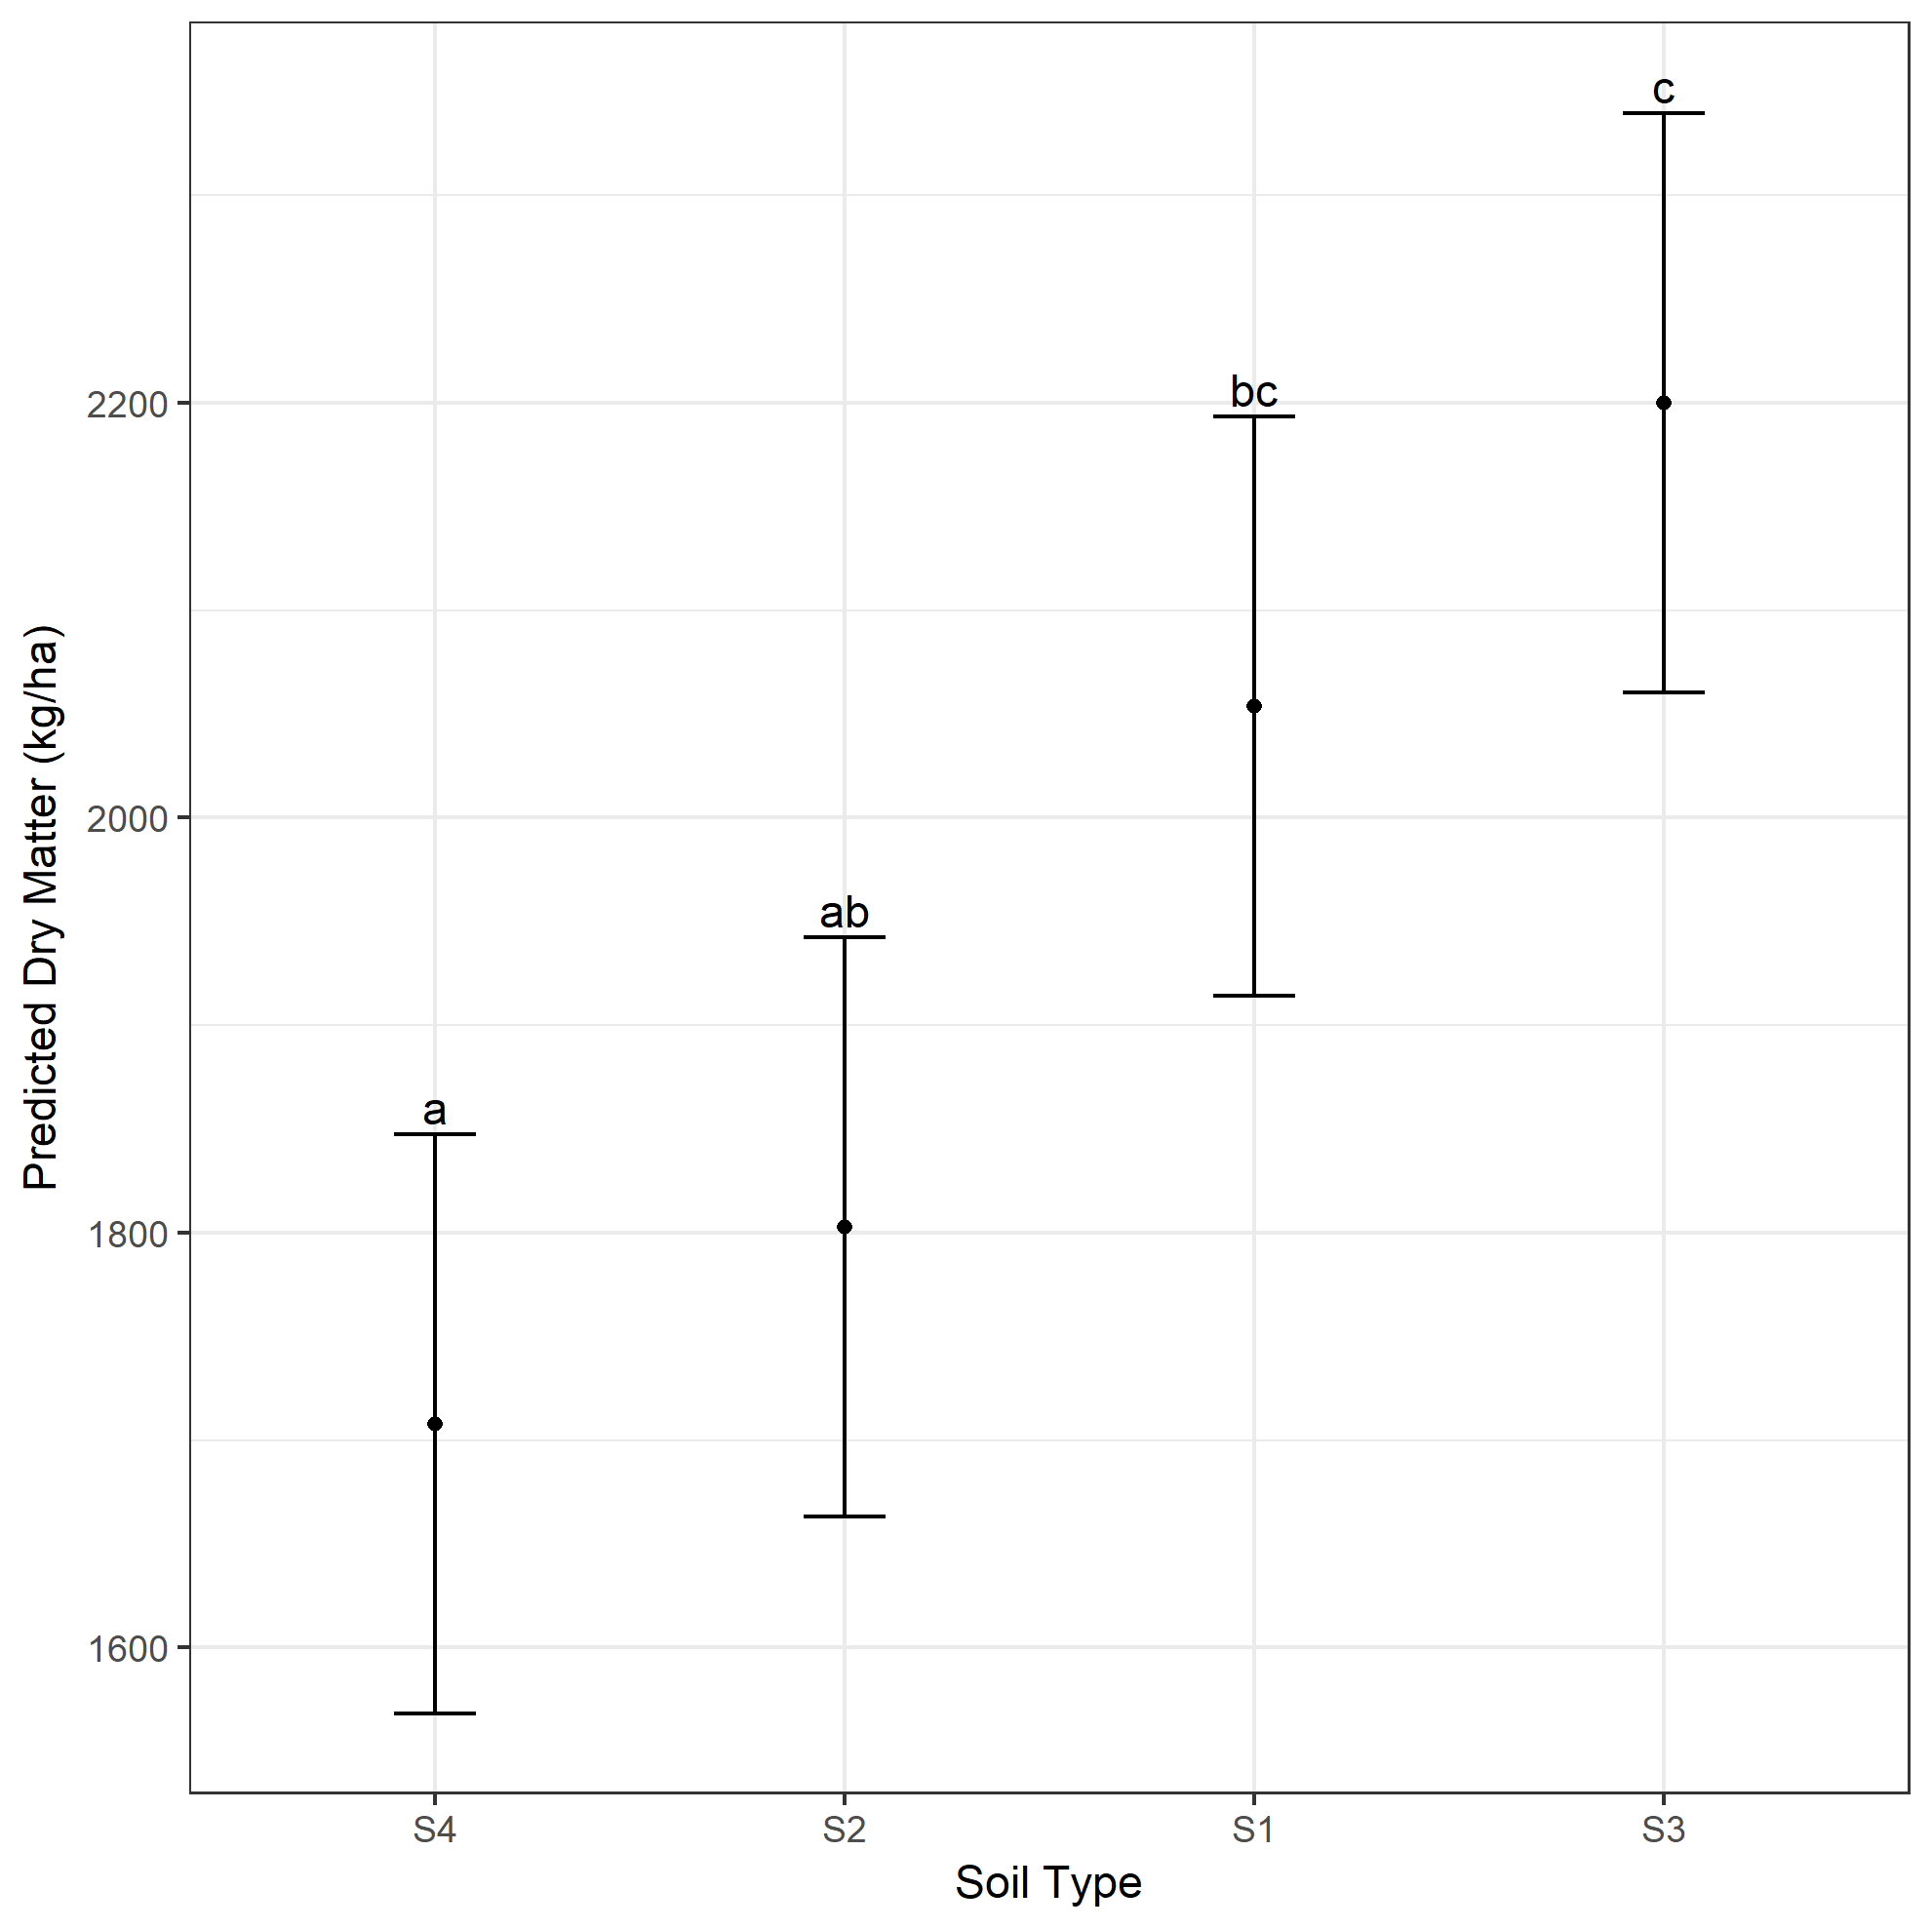
\includegraphics[width=0.8\textwidth, frame]{Example4LMMPred.png}
\end{tcolorbox}

\clearpage
\section{Variance Components}

The variances of the random terms are referred to as the variance components. These can be interpreted in the context
of the analysis even though they are not presented in the ANOVA table. To see a summary of the variance components the
following code is used.

\tcbset {colback = code!10!white, colframe = code}
\begin{tcolorbox}[title = Example 4 Graph of predicted values]
\begin{verbatim}
summary(dat.asr)$varcomp
\end{verbatim}
\end{tcolorbox}

\tcbset {colback = outpt!25!white, colframe = outpt}
\begin{tcolorbox}[title = Example 4 Tukey's multiple comparison output]
\begin{verbatim}
            component    std.error   z.ratio bound %ch
row     1.443632e-02 6.805333e-03 2.1213237     B   0
col     1.104250e+03 4.416586e+03 0.2500234     P   0
plots!R 1.532705e+04 7.225230e+03 2.1213237     P   0

\end{verbatim}
\end{tcolorbox}

There are three variance components presented in this table, the 2 random components that were fitted in the model (row
and column) and the residual variance (R!variance). The variances can be found in the column labelled
\texttt{component}. The variance associated with the residual, $\sigma^2_{res} = 15,327$. The row variance is on the
\texttt{Boundary} (see the \texttt{constraint} column). This means that there is no variance associated with row. The
column variance $\sigma^2_{col} = 1,104$. It is not possible to determine whether this is significant or not from this
table.

\subsection{Likelihood ratio test}

To determine whether the random term in the model are statistically significant, we use a likelihood ratio test, to
test
\begin{eqnarray*}
	H_0&:& \texttt{The reduced model is true} \\
	H_1&:& \texttt{The current model is true}
\end{eqnarray*}
Here to test the null hypothesis that an arbitrary group of $k$ coefficients from the model is set equal to zero (e.g.
no relationship with the response), we need to fit two \textbf{nested} models, the:
\begin{enumerate}
\item \textbf{reduced model} which omits the $k$ predictors in question, and
\item \textbf{current model} which includes them.
\end{enumerate}
The likelihood-ratio test is

\begin{eqnarray*}
\Delta = -2 \times logL \texttt{ from reduced model} - (-2 \times logL \texttt{ from current model})
\end{eqnarray*}


and the degrees of freedom is $k$ (the number of coefficients in question). The $p$-value is $P(\chi^2_k \geq \Delta)$.

As the random terms reflect the design of the experiment, they are left in the model regardless of significance.

The code to do a likelihood ratio test follows:

\tcbset {colback = code!10!white, colframe = code}
\begin{tcolorbox}[title = Example 4 Likelihood Ratio Test]
\begin{verbatim}
library(asremlPlus)
# Note: row is on the boundary

dat.current <- asreml(DM ~ trt, random = ~ col,
residual = ~ id(plots), data = dat)
dat.current <- update(dat.current)

dat.reduced <- asreml(DM ~ trt,
residual = ~ id(plots), data = dat)

dat.reduced <- update(dat.reduced)

REMLRT(h1.asreml.obj = dat.current,
       h0.asreml.obj = dat.reduced)

reml.lrt.asreml(full.asreml.obj = dat.current, reduced.asreml.obj = dat.reduced)
\end{verbatim}
\end{tcolorbox}

\tcbset {colback = outpt!25!white, colframe = outpt}
\begin{tcolorbox}[title = Example 4 Likelihood Ratio Test output]
\begin{verbatim}
      REMLRT DF         p NBound.h0 NBound.h1
1 0.07512287  1 0.7840189         0         0
\end{verbatim}
\end{tcolorbox}

\tcbset {colback = interp!25!white, colframe = interp}
\begin{tcolorbox}[title = Example 4 Likelihood Ratio Test Interpretation]
\begin{verbatim}
Although there is some variance associated with the column
variance component, it is not significant, p-value = 0.784.
\end{verbatim}
\end{tcolorbox}

Most of the time this information is probably not relevant to the aims of the experiment, but it can be informative
from a management perspective.

\textbf{Exercises 7 - 12}


Repeat Exercises 1 - 6 using a LMM. Also, check any random terms for significance using a likelihood ratio test.

\clearpage
\section{Split-plot}

A split-plot design consists of blocks, that contain a complete set of treatments.  Each block divided into whole
plots, with levels of treatment factor A randomised to the whole plots separately with each block. Finally, each whole
plot is divided into a number of subplots and the levels of factor B are randomised onto subplots within each whole
plot.

\textbf{Reminder}

Two factors are crossed when every category of one factor co-occurs in the
design with every category of the other factor. In other words, there is at
least one observation in every combination of levels for the two factors.

A factor is nested within another factor when each level of the first factor
co-occurs with only one level of the other. In other words, an observation has
to be within one level of Factor 2 in order to have a specific level of Factor
1. All combinations of levels are not represented.

If two factors are crossed, you can calculate an interaction. If they are
nested, you cannot because you do not have every combination of one factor
along with every combination of the other.




From the design course we know that the skeletal ANOVA table for a split-plot is partitioned as follows:

\begin{verbatim}
Source of Variation                           df
=============================================================
Block stratum                                 b-1
-------------------------------------------------------------
Whole plot stratum
          Factor A                            t1-1
Whole plot Residual                           (t1-1)(b-1)
=============================================================
Subplot stratum
          Factor B                            t2-1
          Factor A:Factor B                   (t1-1)(t2-1)
          Subplot Residual                    t1(t2-1)(b-1)
=============================================================
Total                                         n-1
\end{verbatim}

where $b$ are the number of blocks, $t1$ are the number of levels in Factor A, $t2$ are the number of levels in Factor
B and $n$ are the total number of observations.

The total variance associated with the data is partitioned into variance associated with Blocks, Whole-plots, Factor A,
Factor B, the interaction of Factor A and B and the residual.

\begin{figure}[!hbtp]
\centering
\fbox{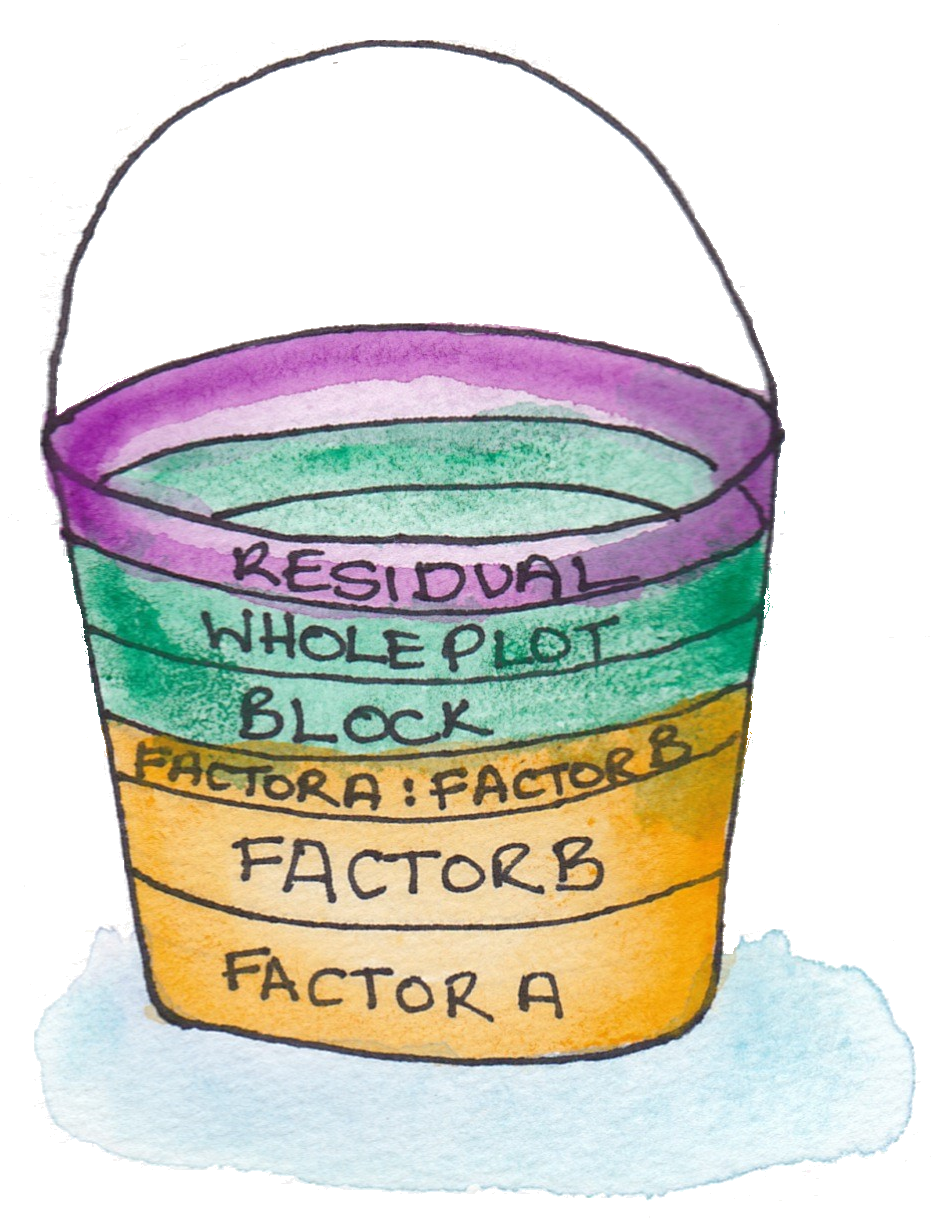
\includegraphics[width = 4cm]{SPBucket.png}}
\caption{Variance partitioning for a Split-plot Design}
\label{fig:spbucket}
\end{figure}

\textbf{Example 5}

The data for the split-plot example is from the \texttt{agridat} package \cite{agridat} and is called
\texttt{durban.splitplot}. The data has been saved to the file \texttt{example5.csv}. The details of the data are as
follows:

\textit{Grown in 1995-1996 at the Scottish Crop Research Institute.   Split-plot design with 4 blocks,  2 whole-plot
fungicide treatments, and 70 barley varieties or variety mixes.  Total area was 10 rows (north/south) by 56 columns
(east/west).}


\begin{application}{Experiment Layout Sketch}
\vspace{10cm}
\end{application}

It is presumed that the aim of this analysis is to determine if the treatments effect the yield, either as a
combination (interaction) or as a main effect.

\clearpage
\subsection{Data Checking}

The code to create the boxplots is given below:

\tcbset {colback = code!10!white, colframe = code}
\begin{tcolorbox}[title = Import and graph the data]
\begin{verbatim}
dat <- read.csv("example5.csv")
dat$WholePlot <- factor(dat$WholePlot)
\end{verbatim}
\tcblower
\begin{verbatim}
ggplot(data = dat, aes(x = Genotype, y = Yield)) + geom_boxplot() +
theme_bw() + theme(axis.text.x = element_text(angle = 90, hjust = 0, size = 6))

ggplot(data = dat, aes(x = Fungicide, y = Yield)) + geom_boxplot() +
theme_bw()

ggplot(data = dat, aes(x = Block, y = Yield)) + geom_boxplot() +
theme_bw()
\end{verbatim}
\end{tcolorbox}


\subsection{Linear Model}
The linear model that is fit can be symbolically written as:
\begin{eqnarray*}
	\texttt{Response variable}&:& \texttt{Yield} \\
	\texttt{Structural component}&:& \texttt{Block, Whole-plot within Block}\\
	\texttt{Explanatory component}&:& \texttt{Genotype, Fungicide}\\
	\texttt{Residual}&:& \texttt{Assume independence}
\end{eqnarray*}


\tcbset {colback = outpt!25!white, colframe = outpt}
\begin{tcolorbox}[title = Example 5 Boxplots]
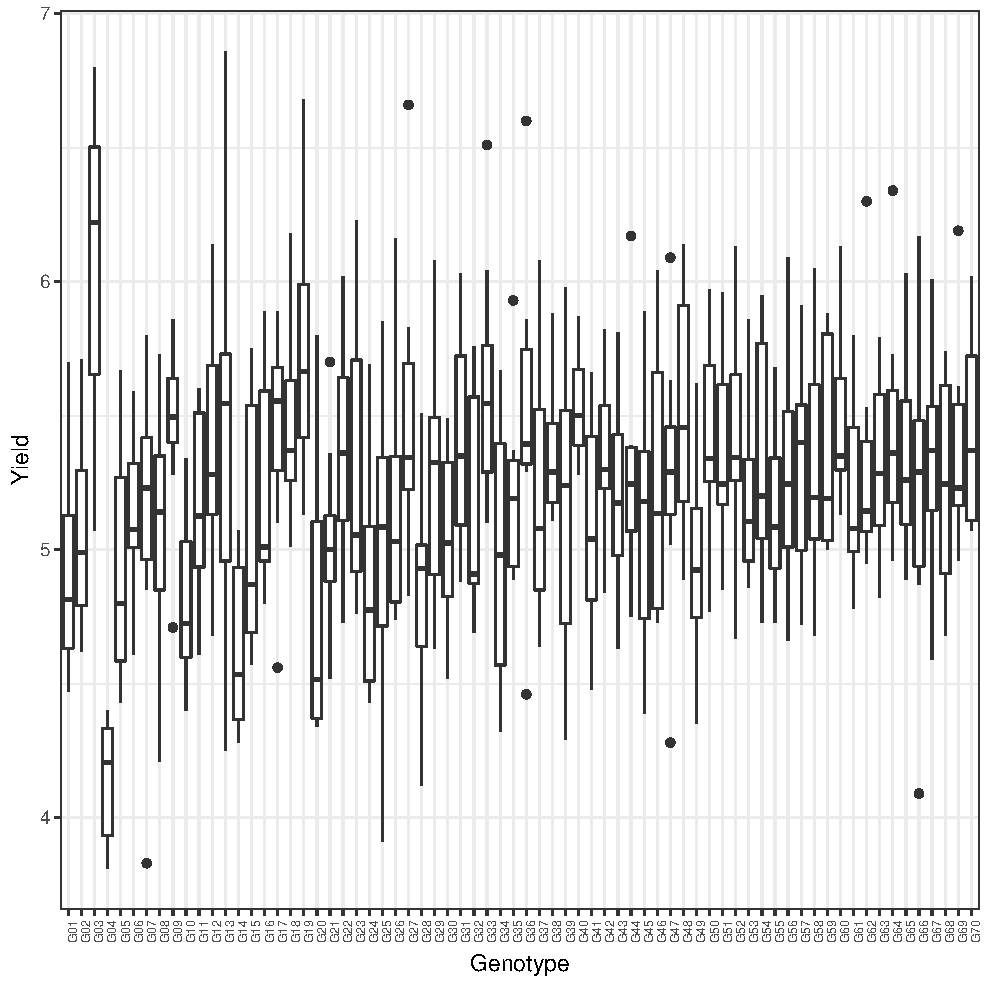
\includegraphics[width=0.5\textwidth, frame]{example5_Genoboxplot.pdf}
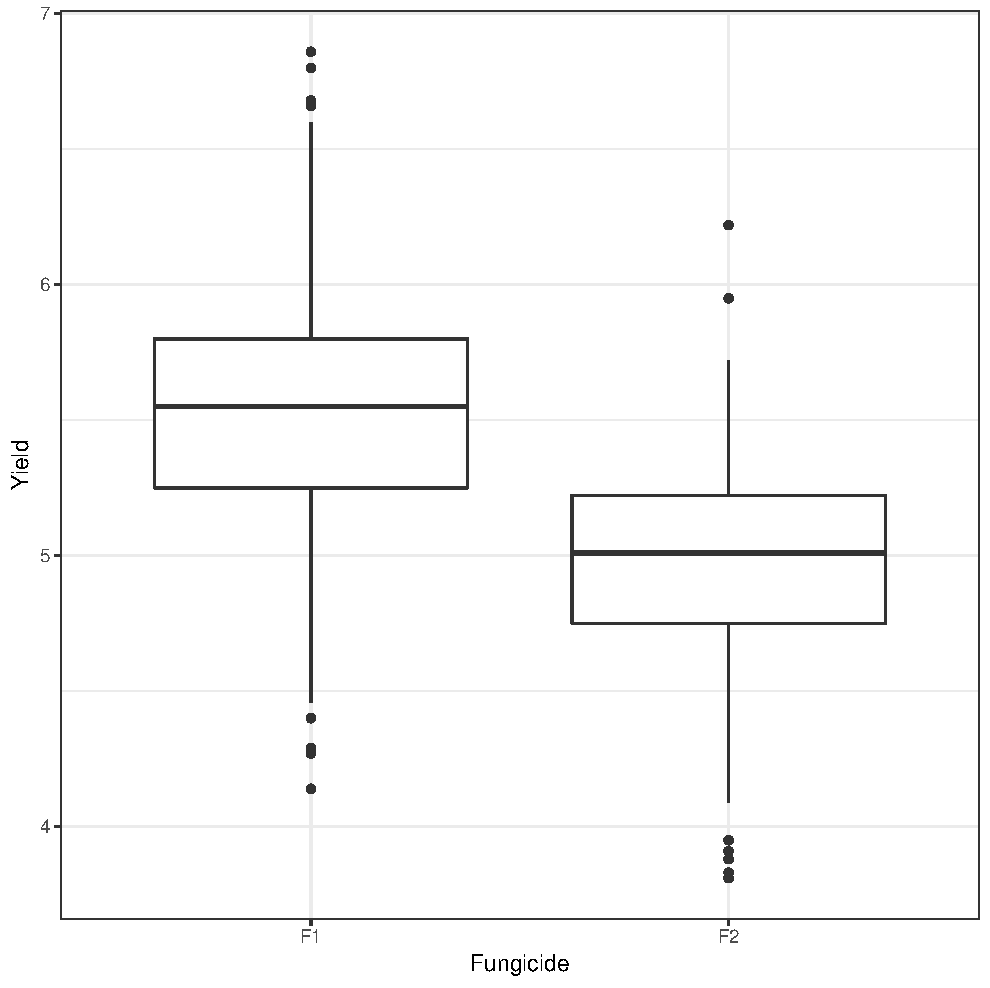
\includegraphics[width=0.5\textwidth, frame]{example5_Fungboxplot.pdf}
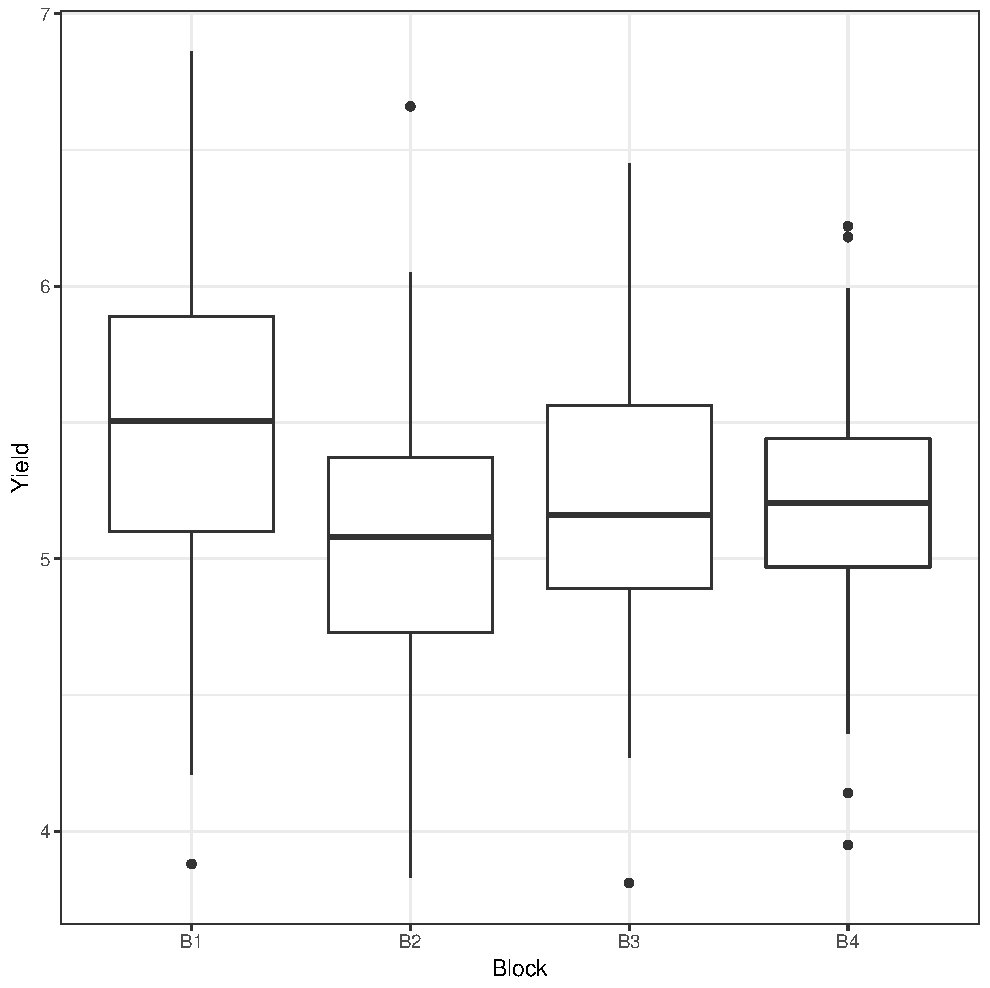
\includegraphics[width=0.5\textwidth, frame]{example5_Blockboxplot.pdf}
\end{tcolorbox}


\subsection{Fitting the Model}

\tcbset {colback = code!10!white, colframe = code}
\begin{tcolorbox}[title = Fitting the linear model for a Split-plot Design]
\begin{verbatim}
# fitting the model
dat.asr <- asreml(Yield ~ Genotype + Fungicide + Genotype:Fungicide,
random = ~ Block + Block:WholePlot,
residual =  ~ units, data = dat)
dat.ww <- wald(dat.asr, denDF = "default")$Wald
\end{verbatim}

\tcblower
\begin{verbatim}
plot(dat.asr)
round(dat.ww,3)
shapiro.test(dat.asr$residuals)
\end{verbatim}
\end{tcolorbox}

\tcbset {colback = outpt!25!white, colframe = outpt}
\begin{tcolorbox}[title = Example 5 Output]
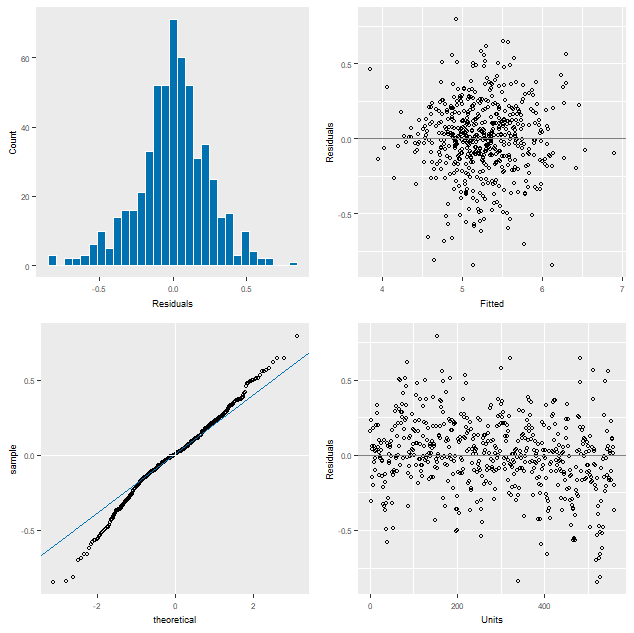
\includegraphics[width=0.8\textwidth, frame]{Example5Resplot.png}
\end{tcolorbox}


\subsection{Interpreting the Output}

The model assumptions need to be verified before the statistical inferences can be considered.

\tcbset {colback = outpt!25!white, colframe = outpt}
\begin{tcolorbox}[title = Example 5 Shapiro-Wilk normality test output]
\begin{verbatim}
Wald tests for fixed effects.
Response: Yield
            Df denDF   F.inc    Pr
(Intercept)  1     3 3029.00 0.000
Fungicide    1     3   40.27 0.008
Genotype    69   483    7.27 0.000

\end{verbatim}

\tcblower

\begin{verbatim}
        Shapiro-Wilk normality test

data:  dat.asr$residuals
W = 0.98183, p-value = 1.915e-06
\end{verbatim}
\end{tcolorbox}

\tcbset {colback = interp!25!white, colframe = interp}
\begin{tcolorbox}[title = Example 5 Output Interpretation]
\begin{verbatim}
Inspection of the residual plots indicates that the model
assumptions are met. Even though there are slight deviations
from a true normal distribution and the Shapiro Wilks
normality test indicates that the residuals are not normally
distributed (p-value < 0.001), the conclusion would be that
the residuals approximately follow a normal distribution.
LMM techniques are robust against departures from normality,
so this would not be considered a serious problem in this
case.

The interaction of Genotype and Fungicide is not significant,
p-value $\ge 0.05$.
\end{verbatim}
\end{tcolorbox}

In this case Genotype and Fungicide are acting independently on Yield, if this
were not the case the interaction term would be significant in the model. When
this  happens the interaction term is removed from the model and the model is
fit again. Of course the model assumptions will need to be checked again as a
different model is now fitted. The main effects of this model are then assessed
for significance.

\tcbset {colback = code!10!white, colframe = code}
\begin{tcolorbox}[title = Fitting the linear model for a Split-plot Design]
\begin{verbatim}
# fitting the model
dat.asr <- asreml(Yield ~ Genotype + Fungicide,
random = ~ Block + Block:WholePlot, residual =  ~ units, data = dat)
dat.ww <- wald(dat.asr, denDF = "default")$Wald
\end{verbatim}

\tcblower
\begin{verbatim}
plot(dat.asr)
round(dat.ww,3)
shapiro.test(dat.asr$residuals)
\end{verbatim}
\end{tcolorbox}

\tcbset {colback = outpt!25!white, colframe = outpt}
\begin{tcolorbox}[title = Example 5 Output]
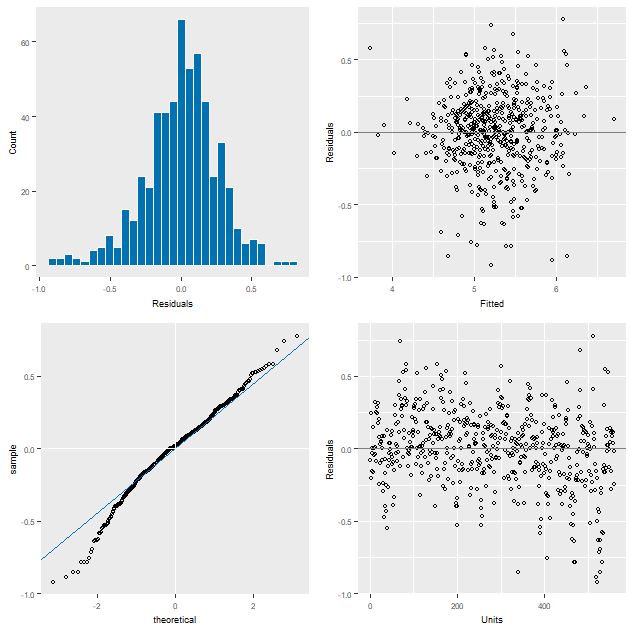
\includegraphics[width=0.8\textwidth, frame]{Example5Resplot2.png}
\end{tcolorbox}

The model assumptions need to be verified before the statistical inferences can be considered.

\tcbset {colback = outpt!25!white, colframe = outpt}
\begin{tcolorbox}[title = Example 5 Shapiro-Wilk normality test output]
\begin{verbatim}
            Df denDF   F.inc    Pr
(Intercept)  1     3 3029.00 0.000
Genotype    69   483    7.27 0.000
Fungicide    1     3   40.27 0.008
\end{verbatim}
\tcblower
\begin{verbatim}
        Shapiro-Wilk normality test

data:  dat.asr$residuals
W = 0.98183, p-value = 1.915e-06
\end{verbatim}
\end{tcolorbox}

\tcbset {colback = interp!25!white, colframe = interp}
\begin{tcolorbox}[title = Example 5 Output Interpretation]
\begin{verbatim}
Inspection of the residual plots indicates that the model
assumptions are met. Even though there are slight deviations
from a true normal distribution and the Shapiro Wilks
normality test indicates that the residuals are not normally
distributed (p-value < 0.001), the conclusion would be that
the residuals approximately follow a normal distribution.
LMM techniques are robust against departures from normality,
so this would not be considered a serious problem in this
case.

The both main effects of Genotype and Fungicide are significant,
p-values < 0.001 and = 0.008, respectively.
\end{verbatim}
\end{tcolorbox}



\subsection{Prediction - Genotype}

As there are two model terms that are significant, two predict statements need to be run. First the predicted values
for Genotype are calculated.

\tcbset {colback = code!10!white, colframe = code}
\begin{tcolorbox}[title = Example 5 predicted values]
\begin{verbatim}
dat.pred <- predict(dat.asr, classify = "Genotype",
sed = TRUE)
\end{verbatim}
\end{tcolorbox}

\subsection{Multiple Comparison Test - Genotype}

\tcbset {colback = code!10!white, colframe = code}
\begin{tcolorbox}[title = Example 5 Tukey's multiple comparison]
\begin{verbatim}
pred.out <- tuk.out(model.obj = dat.asr, pred.obj = dat.pred,
                    pred = "Genotype", sig = 0.95)
pred.out
\end{verbatim}
\end{tcolorbox}
\clearpage


\tcbset {colback = outpt!25!white, colframe = outpt}
\begin{tcolorbox}[title = Example 5 Tukey's multiple comparison output]
\begin{verbatim}
# Truncated output - the first 20 lines only
   predicted.value Genotype std.error     groups        ci      low       up
1          4.14500      G04 0.1367965          a 0.2687815 3.876218 4.413782
2          4.63250      G14 0.1367965         ab 0.2687815 4.363718 4.901282
3          4.79625      G20 0.1367965         bc 0.2687815 4.527468 5.065032
4          4.81250      G10 0.1367965        bcd 0.2687815 4.543718 5.081282
5          4.84000      G28 0.1367965       bcde 0.2687815 4.571218 5.108782
6          4.85500      G24 0.1367965      bcdef 0.2687815 4.586218 5.123782
7          4.91000      G01 0.1367965     bcdefg 0.2687815 4.641218 5.178782
8          4.94250      G05 0.1367965    bcdefgh 0.2687815 4.673718 5.211282
9          4.94750      G49 0.1367965   bcdefghi 0.2687815 4.678718 5.216282
10         5.00625      G34 0.1367965   bcdefghi 0.2687815 4.737468 5.275032
11         5.01625      G25 0.1367965   bcdefghi 0.2687815 4.747468 5.285032
12         5.04250      G30 0.1367965  bcdefghij 0.2687815 4.773718 5.311282
13         5.04750      G21 0.1367965  bcdefghij 0.2687815 4.778718 5.316282
14         5.06250      G02 0.1367965  bcdefghij 0.2687815 4.793718 5.331282
15         5.07125      G15 0.1367965  bcdefghij 0.2687815 4.802468 5.340032
16         5.08750      G41 0.1367965  bcdefghij 0.2687815 4.818718 5.356282
17         5.09000      G08 0.1367965  bcdefghij 0.2687815 4.821218 5.358782
18         5.09875      G07 0.1367965  bcdefghij 0.2687815 4.829968 5.367532
19         5.10625      G45 0.1367965  bcdefghij 0.2687815 4.837468 5.375032
20         5.12625      G06 0.1367965  bcdefghij 0.2687815 4.857468 5.395032
\end{verbatim}
\end{tcolorbox}

\tcbset {colback = code!10!white, colframe = code}
\begin{tcolorbox}[title = Example 5 Graph of predicted values]
\begin{verbatim} 
# graph the predicted values 
ggplot(data = pred.out, aes(x = Genotype)) +
geom_errorbar(aes(ymin = low, ymax = up), width = 0.2) +
geom_text(aes(x = Genotype, y = up, label = groups),
vjust = 0, hjust = 0, nudge_y = 0.05, angle = 90, size = 2) +
geom_point(aes(y = predicted.value), color = "black", shape = 16) + theme_bw() +
labs(x = "", y = "Predicted Yield (t/ha)") +
theme(axis.text.x = element_text(angle = 90, vjust = 0.5, size = 6))
\end{verbatim}
\end{tcolorbox}


\tcbset {colback = outpt!25!white, colframe = outpt}
\begin{tcolorbox}[title = Example 5 Graph of predicted Genotype values]
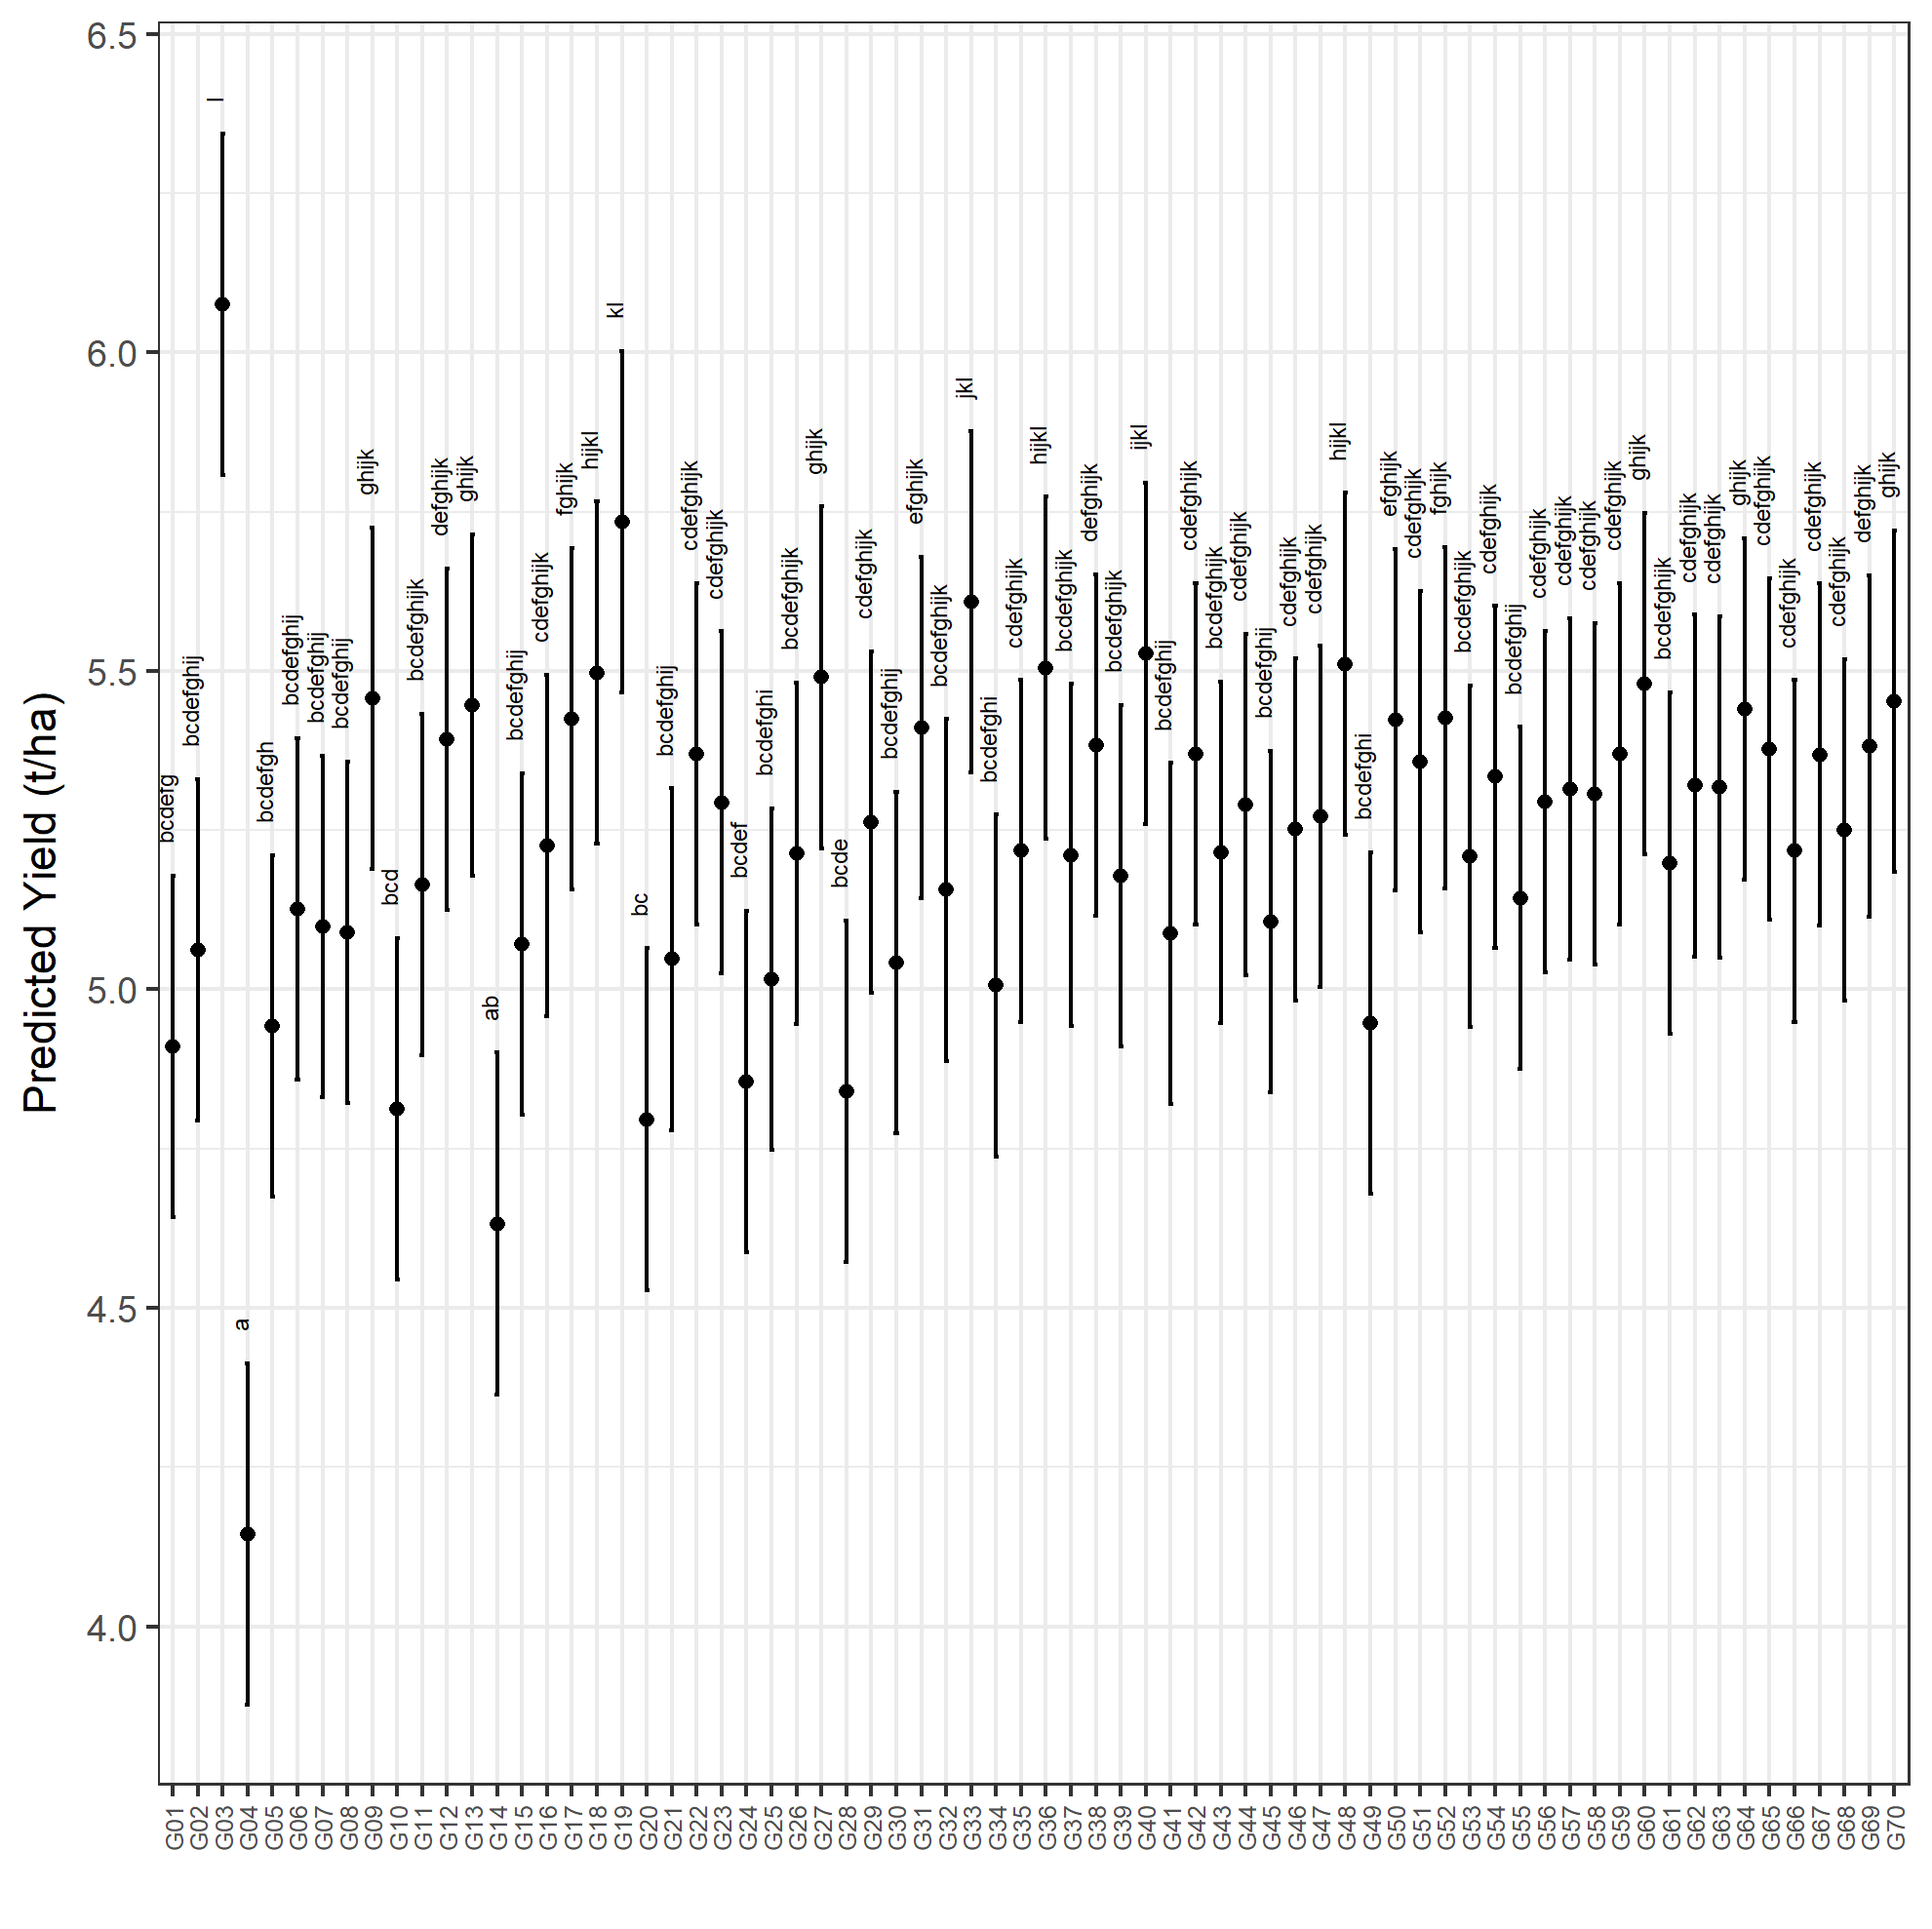
\includegraphics[width=0.8\textwidth, frame]{Example5GenoPred.png}
\end{tcolorbox}


\subsection{Prediction - Fungicide}

Next the predicted values for Fungicide are calculated.

\tcbset {colback = code!10!white, colframe = code}
\begin{tcolorbox}[title = Example 5 predicted values]
\begin{verbatim}
dat.pred <- predict(dat.asr, classify = "Fungicide",
sed = TRUE)
\end{verbatim}
\end{tcolorbox}

\subsection{Multiple Comparison Test - Fungicide}

\tcbset {colback = code!10!white, colframe = code}
\begin{tcolorbox}[title = Example 5 Tukey's multiple comparison]
\begin{verbatim}
pred.out <- tuk.out(model.obj = dat.asr, pred.obj = dat.pred,
                    pred = "Fungicide", sig = 0.95)
pred.out
\end{verbatim}
\end{tcolorbox}
\clearpage


\tcbset {colback = outpt!25!white, colframe = outpt}
\begin{tcolorbox}[title = Example 5 Tukey's multiple comparison output]
\begin{verbatim}
  predicted.value Fungicide std.error groups        ci      low       up
1        4.965786        F2 0.1045358      a 0.2053948 4.760391 5.171180
2        5.513643        F1 0.1045358      b 0.2053948 5.308248 5.719038

\end{verbatim}
\end{tcolorbox}

\tcbset {colback = code!10!white, colframe = code}
\begin{tcolorbox}[title = Example 5 Graph of predicted values]
\begin{verbatim}
# graph the predicted values 
ggplot(data = pred.out, aes(x = Fungicide)) +
geom_errorbar(aes(ymin = low, ymax = up), width = 0.2) +
geom_text(aes(x = Fungicide, y = up, label = groups), vjust = 0, nudge_y = 0.05) +
geom_point(aes(y = predicted.value), color = "black", shape = 16) + theme_bw() +
labs(x = "", y = "Predicted Yield (t/ha)")
\end{verbatim}
\end{tcolorbox}


\tcbset {colback = outpt!25!white, colframe = outpt}
\begin{tcolorbox}[title = Example 5 Graph of predicted Fungicide values]
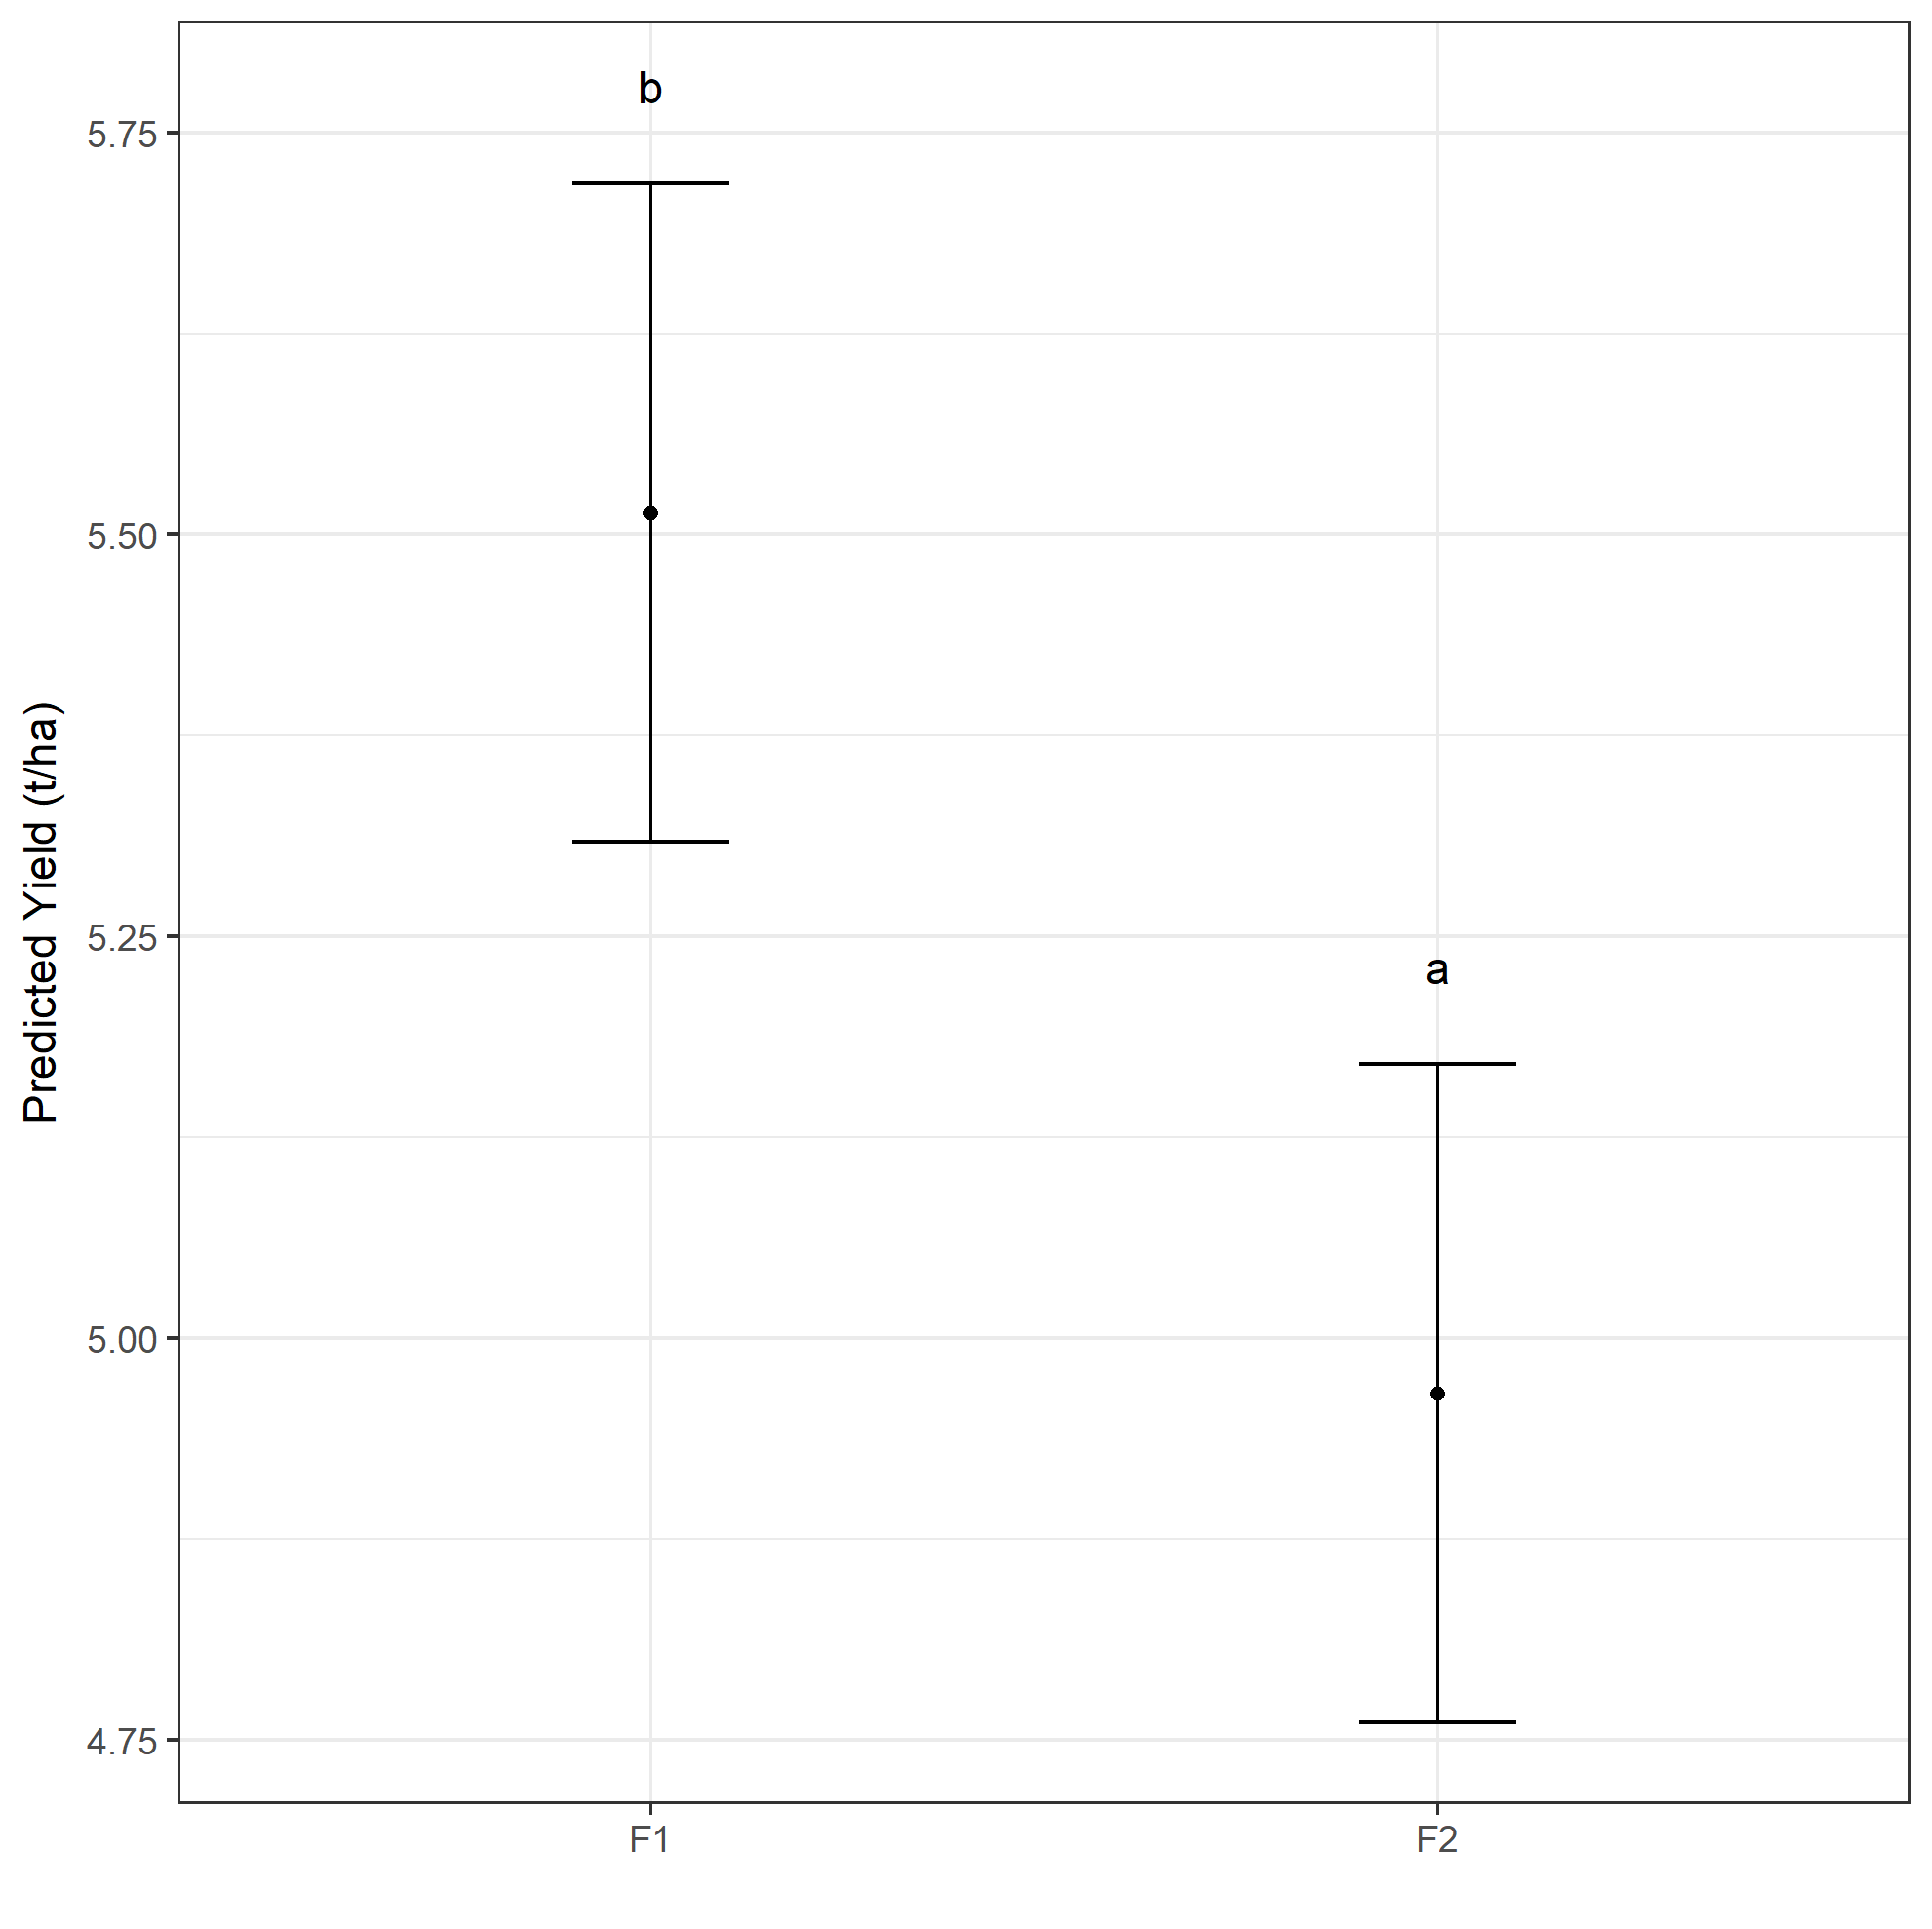
\includegraphics[width=0.8\textwidth, frame]{Example5FungPred.png}
\end{tcolorbox}
\clearpage

\subsection{Likelihood Ratio Test}

\tcbset {colback = code!10!white, colframe = code}
\begin{tcolorbox}[title = Example 5 Likelihood Ratio Test]
\begin{verbatim}
# Likelihood Ratio test for Block:WholePlot

dat.current <- asreml(Yield ~ Genotype + Fungicide,
random = ~ Block + Block:WholePlot, residual = ~ units, data = dat)

dat.reduced <- asreml(Yield ~ Genotype + Fungicide,
random = ~ Block, residual = ~ units, data = dat)

dat.reduced <- update(dat.reduced)


REMLRT(h1.asreml.obj = dat.current,
       h0.asreml.obj = dat.reduced)

\end{verbatim}
\tcblower
\begin{verbatim}
# Likelihood Ratio test for Block

dat.current <- asreml(Yield ~ Genotype + Fungicide,
random = ~ Block, residual = ~ units, data = dat)

dat.current <- update(dat.current)


dat.reduced <- asreml(Yield ~ Genotype + Fungicide,
residual = ~ units, data = dat)

REMLRT(h1.asreml.obj = dat.current,
       h0.asreml.obj = dat.reduced)

\end{verbatim}
\end{tcolorbox}

\tcbset {colback = outpt!25!white, colframe = outpt}
\begin{tcolorbox}[title = Example 5 Likelihood Ratio Test output]
\begin{verbatim}
    REMLRT DF            p NBound.h0 NBound.h1
1 27.86557  1 1.300436e-07         0         0

\end{verbatim}
\tcblower
\begin{verbatim}
    REMLRT DF p NBound.h0 NBound.h1
1 139.2956  1 0         0         0

\end{verbatim}
\end{tcolorbox}

\tcbset {colback = interp!25!white, colframe = interp}
\begin{tcolorbox}[title = Example 4 Likelihood Ratio Test Interpretation]
\begin{verbatim}
The variance associated with both the Block and Whole-plot within
Block variance components is significant, p-values < 0.001.
\end{verbatim}
\end{tcolorbox}


\textbf{Exercise 13}

The data for the split-plot example is from the \texttt{agridat} package \cite{agridat} and is called
\texttt{yates.oats}. The data has been saved to the file \texttt{exercise13.csv}. The details of the data are as
follows:

\textit{The yield of oats from a split-plot field trial conducted at Rothamsted in 1931. Varieties were applied to the
main plots. Manurial (nitrogen) treatments were applied to the sub-plots.}


It is presumed that the aim of this analysis is to determine if the treatments effect the yield (number of 1/4 lbs),
either as a combination (interaction) or as a main effect.

Import the data into R and analyse the data to determine whether Genotype and/or Nitrogen has an effect on yield.


Carry out a complete analysis by:
\begin{enumerate}
  \item Graphing the data to determine whether the centres and the spread are the same or not.
  \item Fit the model to the data.
  \item Check the model assumptions.
  \item Interpret all the output.
  \item Predict the means and the standard errors from the model.
  \item If the variety factor is significant, carry out a Tukey's multiple comparison test and graph the results.
  \item Test whether the random terms are significant .
\end{enumerate}


\textbf{Exercise 14}

In an irrigated canola variety experiment, the first factor is irrigation and it has two levels, rainfed and irrigated.
There are five different canola varieties suited to the environment in which the experiment will be conducted, these
varieties will form the second factor. These varieties are:

\begin{itemize}
\item Bravo
\item Cobbler
\item Hyola
\item Thumper
\item Victory
\end{itemize}

The physical plot area that is available for this experiment is laid out in an array of 6 rows and 5 columns. The rows
will form the main plots for the irrigation treatment and the plots within the row will form the subplots to which the
varieties will be randomised.

The data can be found in \texttt{exercise14.csv}. Import the data into R and analyse the data to determine whether the
treatments have an effect on yield. Carry out a complete analysis by:

\begin{enumerate}
  \item Graphing the data to determine whether the centres and the spread are the same or not.
  \item Fit the model to the data.
  \item Check the model assumptions.
  \item Interpret all the output.
  \item Predict the means and the standard errors from the model.
  \item If the variety factor is significant, carry out a Tukey's multiple comparison test and graph the results.
  \item Test whether the random terms are significant .
\end{enumerate}

\chapter{Extending the model to include spatial modelling}

This section is based on a workshop developed by Beverley Gogel called \emph{Understanding linear mixed models from the
ground up Notes for new biometricians in plant breeding}.

Up until now we have seen simple linear mixed models in which the random model terms and the residual error term are
all assumed to be independently and identically distributed. We call these variance component models. These models
accommodate broad scale variation in the field but they do not capture small scale variation. Field trial data
typically exhibit local variation (also called plot-to-plot variation or spatial trend). This can be due to moisture
gradients and fertility trends in the field. This results in a higher correlation between plots that are closer to each
spatially. In spatial analysis, broad scale variation is accommodated by including appropriate blocking factors as
random terms in the analysis (for example, block in the RCB and both block and row in the LS designs). Alternatively,
spatial variation is accommodated by specifying a more sophisticated spatial covariance structure for the residual
error term. Spatial analysis results in estimated treatment effects that are more accurate and precise than their
counterparts for more traditional methods of analysis.


Local trend reflects that data for plots that are closer together in the experimental layout are more alike than those
that are further apart. As such, the residuals are correlated, with the correlation being a function of the spatial
distance between the plots.

We make some assumptions:

\textbf{Assumption 1}



It is assumed that the correlation for pairs of plots that are the same distance from each other as the crow flies and
irrespective of where they are positioned in the experimental layout, is the same.



\textbf{Assumption 2}



Effects can be indexed by columns and rows. The distance between 2 effects is defined by their separation in the column
and row direction, for example, $\varepsilon_{12}$ and $\varepsilon_{35}$ are 2 apart in the row direction and 3 apart
in the column direction. It is assumed that the correlation between 2 smooth trend effects is the product of the
correlation between the column effects of their separation in columns and the correlation between the row effects of
their separation in rows. We call this the assumption of separability. The assumption of separability is
computationally convenient and appears to be reasonable for the two-dimensional smooth trend process associated with
field trials.




Many forms for modelling the spatial correlation are possible. After the analysis of many hundred field trails, a
separable autoregressive spatial model of order 1 (AR1 $\times$ AR1) is a plausible model for smooth trend in field
trial analysis.


\clearpage

There are special rules that apply to specifying the spatial variance structure for the residual error term:

\textbf{Rule 1}

The number of effects in the residual term must be equal to the number of data units included in the analysis.


\textbf{Rule 2}

Where a compound model term is specified for the residuals, each combination of levels of the factors comprising this
term must uniquely identify one unit of the data.

\textbf{Rule 3}

The data must be ordered to match the R structure specified.



Rule 1 and Rule 2 would be broken if there were missing values in either the response or the explanatory variables for
every column by row combination. Rule 3 would be broken if the data were ordered as columns within rows.

\textbf{Rule 4}

Never fit an autoregressive correlation structure for less than 5 rows or
columns.

\textbf{Example 6}

A field trial to test the response of a crop to herbicide treatments was
designed as a RCBD with three blocks of 21 plots. The yield at harvest was
recorded for each plot.  The data can be found in \texttt{example6.csv}. Is
there any evidence of differences in yield among the herbicide treatments?


\begin{application}{Experiment Layout Sketch}
\vspace{10cm}
\end{application}


\subsection{Data Checking}

The code to create the boxplots is given below:

\tcbset {colback = code!10!white, colframe = code}
\begin{tcolorbox}[title = Import and graph the data]
\begin{verbatim}
dat <- read.csv("example6.csv")

dat$Row <- factor(dat$Row)
dat$Column <- factor(dat$Column)
dat$Block <- factor(dat$Block)
\end{verbatim}
\tcblower
\begin{verbatim}
ggplot(data = dat, aes(x = Treatment, y = Yield)) + geom_boxplot() +
theme_bw()

ggplot(data = dat, aes(x = Block, y = Yield)) + geom_boxplot() +
theme_bw()
\end{verbatim}
\end{tcolorbox}


\subsection{Linear Mixed Model}
The linear model that is fit can be symbolically written as:
\begin{eqnarray*}
	\texttt{Response variable}&:& \texttt{Yield} \\
	\texttt{Structural component}&:& \texttt{Block}\\
	\texttt{Explanatory component}&:& \texttt{Treatment}\\
	\texttt{Residual}&:& \texttt{Explore spatial correlation}
\end{eqnarray*}
The modelling process is altered by fitting an ID $\times$ AR1 process to accommodate a smooth spatial trend.

\tcbset {colback = outpt!26!white, colframe = outpt}
\begin{tcolorbox}[title = Example 6 Boxplots]
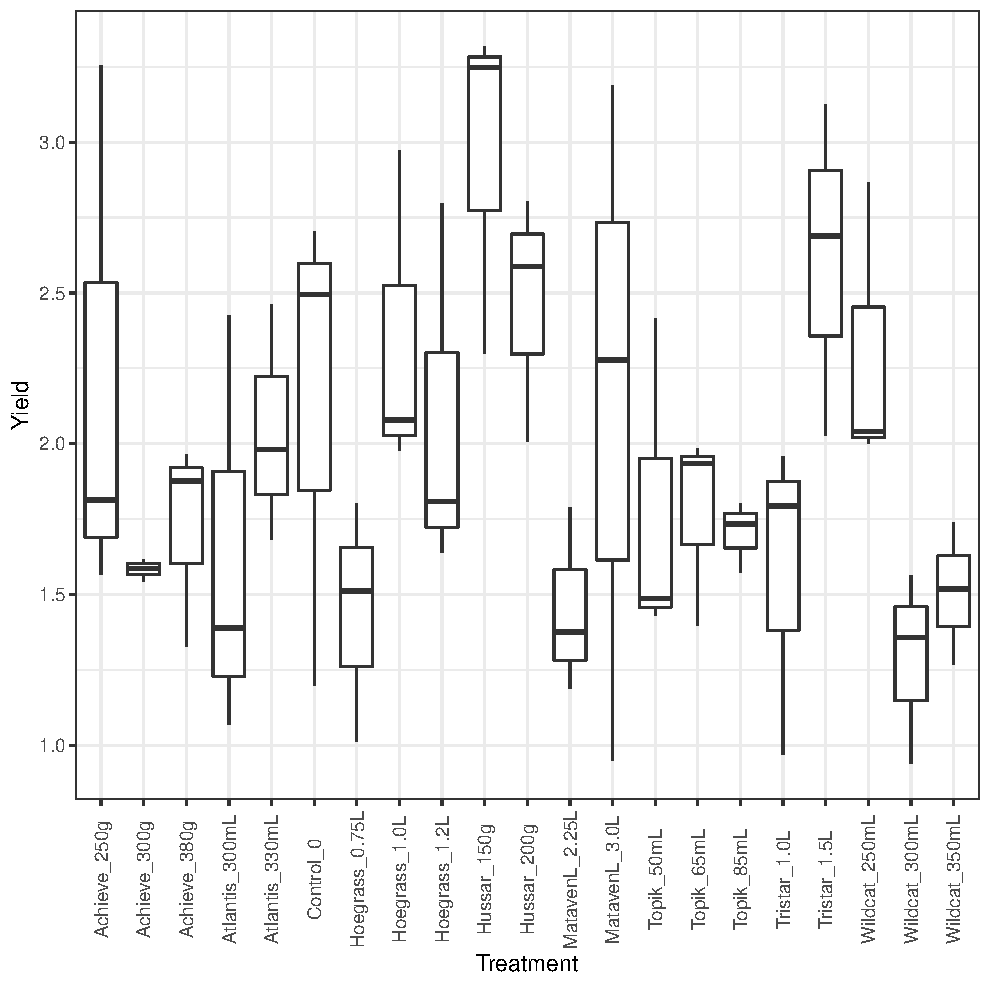
\includegraphics[width=0.6\textwidth, frame]{example6_Treatboxplot.pdf}
\tcblower
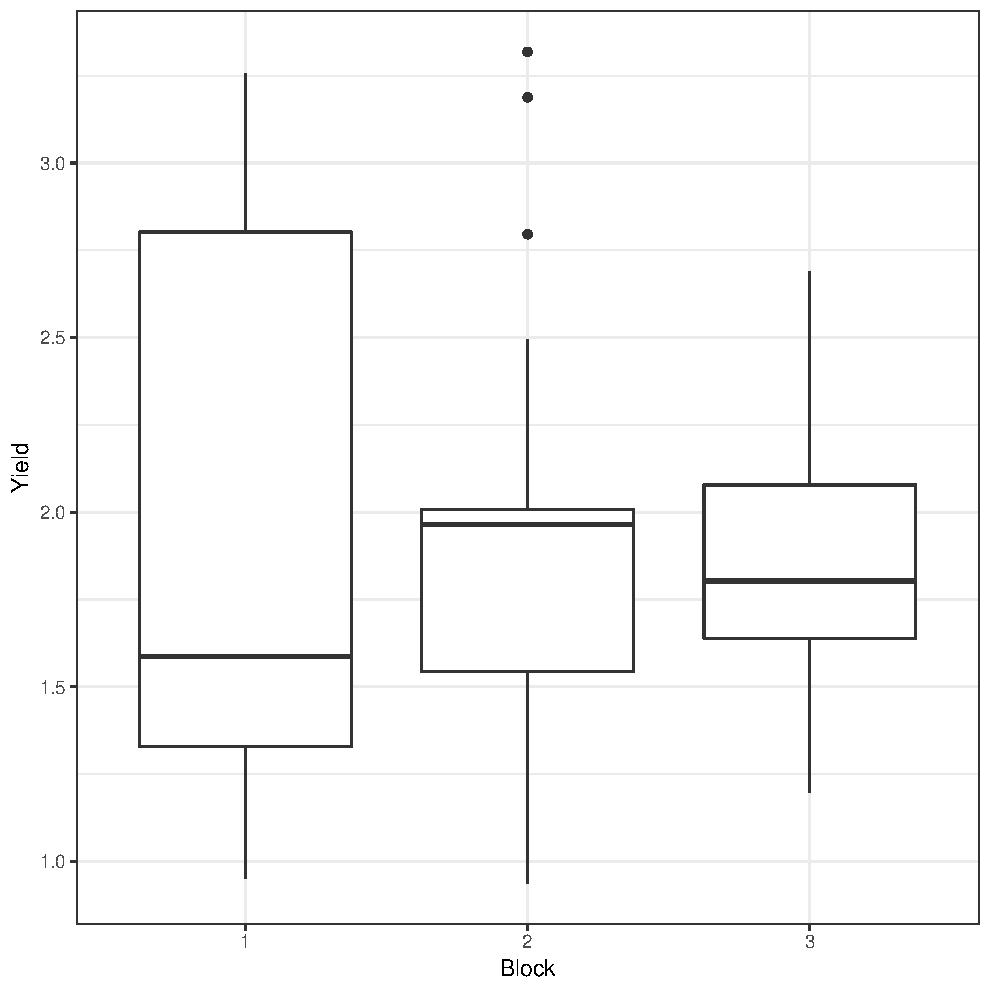
\includegraphics[width=0.6\textwidth, frame]{example6_Blockboxplot.pdf}
\end{tcolorbox}


\subsection{Fitting the Model}

\tcbset {colback = code!10!white, colframe = code}
\begin{tcolorbox}[title = Fitting the linear model for a Split-plot Design]
\begin{verbatim}
# fitting the model
dat.asr <- asreml(Yield ~ Treatment, random = ~ Block,
residual = ~ id(Column):ar1(Row), data = dat)

dat.ww <- wald(dat.asr, denDF = "default")$Wald

\end{verbatim}

\tcblower
\begin{verbatim}
plot(dat.asr)
round(dat.ww,3)
shapiro.test(dat.asr$residuals)
\end{verbatim}
\end{tcolorbox}

\tcbset {colback = outpt!26!white, colframe = outpt}
\begin{tcolorbox}[title = Example 6 Output]
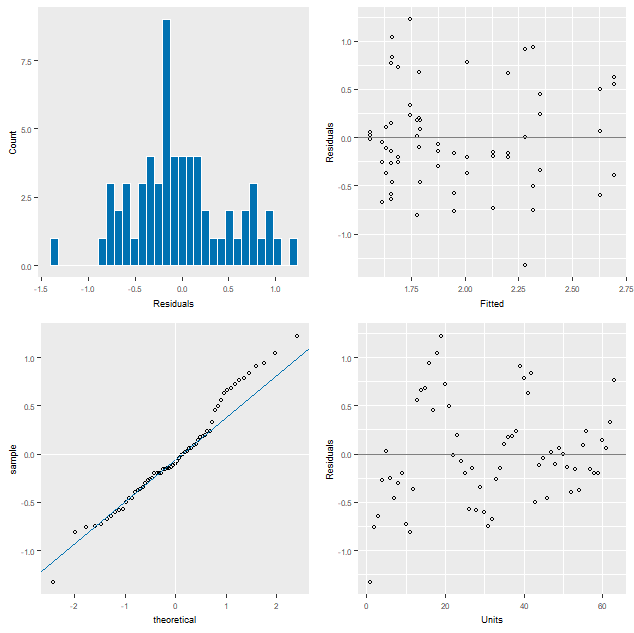
\includegraphics[width=0.8\textwidth, frame]{Example6Resplot.png}
\end{tcolorbox}


\subsection{Interpreting the Output}

The model assumptions need to be verified before the statistical inferences can be considered.

\tcbset {colback = outpt!26!white, colframe = outpt}
\begin{tcolorbox}[title = Example 6 Shapiro-Wilk normality test output]
\begin{verbatim}
 Wald tests for fixed effects.
Response: Yield

            Df denDF   F.inc    Pr
(Intercept)  1   4.0 106.000 0.000
Treatment   20  30.6   3.036 0.003

\end{verbatim}
\tcblower

\begin{verbatim}
        Shapiro-Wilk normality test

data:  dat.asr$residuals
W = 0.97739, p-value = 0.2978

\end{verbatim}
\end{tcolorbox}


\textbf{Assumption 3}

The assumption of independence is no longer relevant - when a spatial model is fitted it is assumed that the residuals
are dependent.

\tcbset {colback = interp!26!white, colframe = interp}
\begin{tcolorbox}[title = Example 6 Output Interpretation]
\begin{verbatim}

Inspection of the residual plots indicates that the model
assumptions are met. The Shapiro Wilks normality test indicates
that the residuals are normally distributed (p-value < 0.05).

The main effect of Treatment is significant, p-value < 0.001.
\end{verbatim}
\end{tcolorbox}

\subsection{Variogram}
A variogram is a graph of the spatial continuity of the data. The experimental
variogram is a discrete function calculated using a measure of variability
between pairs of points at various distances. The distances between pairs at
which the variogram is calculated are called lags .

\tcbset {colback = code!10!white, colframe = code}
\begin{tcolorbox}[title = Producing a variogram]
\begin{verbatim}
plot(varioGram(dat.asr))
\end{verbatim}
\end{tcolorbox}

\tcbset {colback = outpt!26!white, colframe = outpt}
\begin{tcolorbox}[title = Example 6 Variogram]
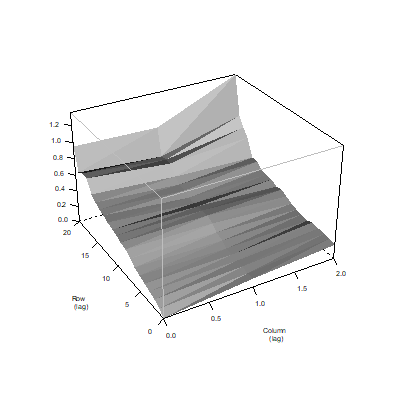
\includegraphics[width=0.8\textwidth, frame]{Example6Variogram.png}
\end{tcolorbox}

\tcbset {colback = interp!26!white, colframe = interp}
\begin{tcolorbox}[title = Example 6 Variogram Interpretation]
\begin{verbatim}
There appears to be a linear trend in the row direction.
\end{verbatim}
\end{tcolorbox}

\subsection{Prediction}

\tcbset {colback = code!10!white, colframe = code}
\begin{tcolorbox}[title = Example 6 predicted values]
\begin{verbatim}
dat.pred <- predict(dat.asr, classify = "Treatment",
sed = TRUE)
\end{verbatim}
\end{tcolorbox}

\subsection{Multiple Comparison Test}

\tcbset {colback = code!10!white, colframe = code}
\begin{tcolorbox}[title = Example 6 Tukey's multiple comparison]
\begin{verbatim}
pred.out <- tuk.out(model.obj = dat.asr, pred.obj = dat.pred,
                        pred = "Treatment", sig = 0.95)
pred.out
\end{verbatim}
\end{tcolorbox}
\clearpage


\tcbset {colback = outpt!26!white, colframe = outpt}
\begin{tcolorbox}[title = Example 6 Tukey's multiple comparison output]
\begin{verbatim}
   predicted.value      Treatment std.error groups        ci      low       up
1         1.560548   Achieve_300g 0.2672702      a 0.5393731 1.021175 2.099921
2         1.613703  Wildcat_300mL 0.2629203      a 0.5305947 1.083108 2.144298
3         1.634260  Wildcat_350mL 0.2642979      a 0.5333747 1.100885 2.167634
4         1.657113 Hoegrass_0.75L 0.2648059      a 0.5344000 1.122713 2.191513
5         1.657669 Atlantis_300mL 0.2681999     ab 0.5412494 1.116419 2.198918
6         1.660627      Control_0 0.2670224      a 0.5388730 1.121754 2.199500
7         1.690366     Topik_50mL 0.2625707     ab 0.5298892 1.160477 2.220256
8         1.747527  Hoegrass_1.0L 0.2619068     ab 0.5285493 1.218978 2.276077
9         1.777929   Tristar_1.0L 0.2633748     ab 0.5315118 1.246417 2.309441
10        1.785587 Atlantis_330mL 0.2622080     ab 0.5291572 1.256429 2.314744
11        1.789971   Achieve_380g 0.2648037     ab 0.5343955 1.255576 2.324367
12        1.876730     Topik_85mL 0.2667394     ab 0.5383020 1.338428 2.415032
13        1.951260 MatavenL_2.25L 0.2668934     ab 0.5386127 1.412648 2.489873
14        2.013181  Hoegrass_1.2L 0.2677548     ab 0.5403511 1.472830 2.553532
15        2.132837     Topik_65mL 0.2653032     ab 0.5354036 1.597433 2.668240
16        2.203311  Wildcat_250mL 0.2648805     ab 0.5345506 1.668760 2.737861
17        2.278864  MatavenL_3.0L 0.2679992     ab 0.5408443 1.738020 2.819708
18        2.317689   Achieve_250g 0.2680859     ab 0.5410193 1.776670 2.858708
19        2.350540    Hussar_200g 0.2612771     ab 0.5272786 1.823261 2.877818
20        2.627455   Tristar_1.5L 0.2665067     ab 0.5378323 2.089623 3.165287
21        2.694812    Hussar_150g 0.2662682      b 0.5373510 2.157461 3.232163

\end{verbatim}
\end{tcolorbox}

\tcbset {colback = code!10!white, colframe = code}
\begin{tcolorbox}[title = Example 6 Graph of predicted values]
\begin{verbatim}
# graph the predicted values 
ggplot(data = pred.out, aes(x = Treatment)) +
geom_errorbar(aes(ymin = low, ymax = up), width = 0.2) +
geom_text(aes(x = Treatment, y = up, label = groups),
vjust = 0, angle = 90, nudge_y = 0.1) +
geom_point(aes(y = predicted.value), color = "black", shape = 16) +
theme_bw() +
labs(x = "", y = "Predicted Yield (t/ha)") +
theme(axis.text.x = element_text(angle = 90, hjust = 0, size = 8))
\end{verbatim}
\end{tcolorbox}


\tcbset {colback = outpt!26!white, colframe = outpt}
\begin{tcolorbox}[title = Example 6 Graph of predicted Treatment values]
\includegraphics[width=0.8\textwidth, frame]{Example6Pred.png}
\end{tcolorbox}
\clearpage

\subsection{Likelihood Ratio Test}

\tcbset {colback = code!10!white, colframe = code}
\begin{tcolorbox}[title = Example 6 Variance Components]
\begin{verbatim}
summary(dat.asr)$varcomp
\end{verbatim}
\end{tcolorbox}

\tcbset {colback = outpt!26!white, colframe = outpt}
\begin{tcolorbox}[title = Example 6 Variance Component output]
\begin{verbatim}
                      component    std.error  z.ratio bound %ch
Block              6.096306e-07 2.392077e-07 2.548541     B   0
Column:Row!R       3.810191e-01 1.495048e-01 2.548541     P   0
Column:Row!Row!cor 7.795568e-01 9.457545e-02 8.242698     U   0
\end{verbatim}
\end{tcolorbox}


\tcbset {colback = code!10!white, colframe = code}
\begin{tcolorbox}[title = Example 6 Likelihood Ratio Test]
\begin{verbatim}
# Likelihood Ratio test for ar1(Row)

dat.current <- asreml(Yield ~ Treatment,
random = ~ Block, residual = ~ id(Column):ar1(Row), data = dat)

dat.reduced <- asreml(Yield ~ Treatment,
random = ~ Block, residual = ~ id(Column):id(Row), data = dat)

dat.reduced <- update(dat.reduced)

REMLRT(h1.asreml.obj = dat.current,
       h0.asreml.obj = dat.reduced)

\end{verbatim}
\end{tcolorbox}

\tcbset {colback = outpt!26!white, colframe = outpt}
\begin{tcolorbox}[title = Example 6 Likelihood Ratio Test output]
\begin{verbatim}
# Likelihood Ratio test for ar1(Row)
    REMLRT DF            p NBound.h0 NBound.h1
1 21.29566  1 3.936222e-06         1         1
Warning message:
In DFdiff(bound.h1, bound.h0, DF = DF, bound.exclusions = bound.exclusions) :
  There were a total of 1 bound terms. These bound terms occur in both models

\end{verbatim}
\end{tcolorbox}

\tcbset {colback = interp!26!white, colframe = interp}
\begin{tcolorbox}[title = Example 6 Likelihood Ratio Test Interpretation]
\begin{verbatim}
The residuals show evidence of autoregressive correlation in
the row direction, p-value < 0.001.
\end{verbatim}
\end{tcolorbox}

\clearpage
\textbf{Exercise 15}

Repeat the analysis of Exercise 13 adding a spatial correlation component.
Also, check all random terms for significance using a likelihood ratio test.


\textbf{Exercise 16}

A RCBD experiment on wheat was conducted in El Batan, Mexico.  There are three
replicates with 50 varieties in each replicate. The data are from the
\texttt{agridat} package \cite{agridat} and is called \texttt{besag.elbatan}.
The data has been saved to the file \texttt{exercise16.csv}.

Import the data into R and analyse the data to determine whether the treatments
have an effect on yield. Carry out a complete spatial analysis by:

\begin{enumerate}
  \item Graphing the data to determine whether the centres and the spread are
      the same or not.
  \item Fit the model to the data.
  \item Check the model assumptions.
  \item Interpret all the output.
  \item Predict the means and the standard errors from the model.
  \item If the variety factor is significant, carry out a Tukey's multiple
      comparison test and graph the results.
  \item Test whether the random terms are significant.
  \item Test which spatial model is the ``best'' one to use.
\end{enumerate}


\chapter[Modelling complex treatment structures]{Extending the model to include more complex treatment structures}

In the design workshop we saw that it was possible to plan experiments with more than one treatment variable. We have
seen the analysis of a split-plot experiment where there was a factorial treatment structure with two explanatory
variables. There are other more complex treatment structures that can be used when analysing experimental data.

For example, Example 6 had 21 herbicide treatments, one of which was a control. The treatments were:

\begin{enumerate}
\item  Achieve\_250g
\item  Achieve\_300g
\item  Achieve\_380g
\item  Atlantis\_300mL
\item  Atlantis\_330mL
\item  Control\_0
\item  Hoegrass\_0.75L
\item  Hoegrass\_1.0L
\item  Hoegrass\_1.2L
\item  Hussar\_150g
\item  Hussar\_200g
\item  MatavenL\_2.25L
\item  MatavenL\_3.0L
\item  Topik\_50mL
\item  Topik\_65mL
\item  Topik\_85mL
\item  Tristar\_1.0L
\item  Tristar\_1.5L
\item  Wildcat\_250mL
\item  Wildcat\_300mL
\item  Wildcat\_350mL
\end{enumerate}

The simple hypothesis was tested:

\begin{eqnarray*}
	H_0&:& \texttt{Yield is the same for all Treatments} \\
	H_1&:& \texttt{Yield is not the same for all Treatments}
\end{eqnarray*}

It can be seen that the 21 treatments are made up of 8 different herbicides with 2 or 3 different rates of application
within a herbicide. This treatment structure would have been purposefully made, specifically to answer the following
hypotheses:

\begin{eqnarray*}
	H_0&:& \texttt{Yield is the same for the Control and the Treatments} \\
	H_1&:& \texttt{Yield is not the same for the Control and the Treatments}
\end{eqnarray*}

\begin{eqnarray*}
	H_0&:& \texttt{Yield is not affected by the different Herbicide Treatments} \\
	H_1&:& \texttt{Yield is affected by the different Herbicide Treatments}
\end{eqnarray*}

\begin{eqnarray*}
	H_0&:& \texttt{Yield is not affected differently by rate of application within the Herbicide Treatments} \\
	H_1&:& \texttt{Yield is affected differently by rate of application within the Herbicide Treatments}
\end{eqnarray*}

To fit a model to answer these three hypotheses the data must contain a separate columns for Control (Yes/No),
Herbicide (Achieve, Atlantis, Control, Hoegrass, Hussar, MatavenL, Topik, Tristar \& Wildcat) and Application Rate.
Each column relates to each of the hypotheses.


\textbf{Example 7}

This example is based on the data from Example 6 but contains the columns required to complete the data analysis to
answer the three hypotheses stated. The data can be found in \texttt{example7.csv}.

\begin{application}{Experiment Layout Sketch}
\vspace{10cm}
\end{application}


The code to create the boxplots is given below:

\tcbset {colback = code!10!white, colframe = code}
\begin{tcolorbox}[title = Import and graph the data]
\begin{verbatim}
dat <- read.csv("example7.csv")

dat$Row <- factor(dat$Row)
dat$Column <- factor(dat$Column)
dat$Block <- factor(dat$Block)
\end{verbatim}
\tcblower
\begin{verbatim}
ggplot(data = dat, aes(x = Herbicide, y = Yield)) + geom_boxplot() +
theme_bw()

ggplot(data = dat, aes(x = Rate, y = Yield)) + geom_boxplot() +
theme_bw()

ggplot(data = dat, aes(x = Block, y = Yield)) + geom_boxplot() +
theme_bw()
\end{verbatim}
\end{tcolorbox}

\subsection{Linear Mixed Model}
The linear model that is fit can be symbolically written as:
\begin{eqnarray*}
	\texttt{Response variable}&:& \texttt{Yield} \\
	\texttt{Structural component}&:& \texttt{Block}\\
	\texttt{Explanatory component}&:& \texttt{Control, Herbicide, Herbicide:Rate}\\
    \texttt{Residual}&:& \texttt{Explore spatial correlation}
\end{eqnarray*}
The modelling process is altered by fitting an ID $\times$ AR1 process to
accommodate a smooth spatial trend.

\tcbset {colback = outpt!26!white, colframe = outpt}
\begin{tcolorbox}[title = Example 7 Boxplots]
\includegraphics[width=0.6\textwidth, frame]{example7_Herbboxplot.pdf}
{\color{outpt} {\hrule height 1pt}}
\includegraphics[width=0.6\textwidth, frame]{example7_Rateboxplot.pdf}
\end{tcolorbox}


\subsection{Fitting the Model}

\tcbset {colback = code!10!white, colframe = code}
\begin{tcolorbox}[title = Fitting the linear mixed model]
\begin{verbatim}
# fitting the model
dat.asr <- asreml(Yield ~ Control + Herbicide + Herbicide:Rate,
random = ~ Block,  residual = ~ id(Column):ar1(Row), data = dat)

dat.ww <- wald(dat.asr, denDF = "default")$Wald
\end{verbatim}

\tcblower
\begin{verbatim}
plot(dat.asr)
round(dat.ww,3)
shapiro.test(dat.asr$residuals)
plot(varioGram(dat.asr))
\end{verbatim}
\end{tcolorbox}

\tcbset {colback = outpt!26!white, colframe = outpt}
\begin{tcolorbox}[title = Example 7 Output]
\includegraphics[width=0.8\textwidth, frame]{Example7Resplot.png}
\begin{verbatim}
Wald tests for fixed effects.
Response: Yield

               Df denDF   F.inc    Pr
(Intercept)     1   4.0 106.000 0.000
Control         1  32.0   3.904 0.057
Herbicide       7  30.3   3.514 0.007
Herbicide:Rate 12  31.0   2.684 0.013
\end{verbatim}
\end{tcolorbox}


\subsection{Interpreting the Output}

The model assumptions need to be verified before the statistical inferences can be considered.

\tcbset {colback = outpt!26!white, colframe = outpt}
\begin{tcolorbox}[title = Example 7 Shapiro-Wilk normality test output]
\begin{verbatim}
        Shapiro-Wilk normality test

data:  dat.asr$residuals
W = 0.97739, p-value = 0.2978
\end{verbatim}
\end{tcolorbox}


\textbf{Assumption 3}

The assumption of independence is no longer relevant - when a spatial model is fitted the residuals are dependent.

\tcbset {colback = interp!26!white, colframe = interp}
\begin{tcolorbox}[title = Example 7 Output Interpretation]
\begin{verbatim}

Inspection of the residual plots indicates that the model
assumptions are met. The Shapiro Wilks normality test indicates
that the residuals are normally distributed (p-value $\ge\ 0.05$).

The Control is different to the other Treatments, p-value < 0.001.
There are differences in yield due to the Herbicide Treatment,
p-value < 0.001. Also, there are differences in Yield due to the
different application Rates within Herbicide, p-value = 0.002.
\end{verbatim}
\end{tcolorbox}


\subsection{Variogram}


\tcbset {colback = outpt!26!white, colframe = outpt}
\begin{tcolorbox}[title = Example 7 Variogram]
\includegraphics[width=0.6\textwidth, frame]{Example6Variogram.png}
\end{tcolorbox}


\subsection{Prediction}

\tcbset {colback = code!10!white, colframe = code}
\begin{tcolorbox}[title = Example 7 predicted values]
\begin{verbatim}
dat.pred <- predict(dat.asr, classify = "Herbicide",
present = c("Control", "Herbicide", "Rate"), sed = TRUE)
\end{verbatim}
{\color{code} {\hrule height 1pt}}
\begin{verbatim}
dat.pred <- predict(dat.asr, classify = "Herbicide:Rate",
present = c("Control", "Herbicide", "Rate"), sed = TRUE)
\end{verbatim}
\end{tcolorbox}

The \texttt{present} statement is required as this is not a balanced design with respect to Herbicide and Rate. When
this happens the fixed effects from the model should be included in the \texttt{present} statement.

\subsection{Multiple Comparison Test}

\tcbset {colback = code!10!white, colframe = code}
\begin{tcolorbox}[title = Example 7 Tukey's multiple comparison]
\begin{verbatim}
pred.out <- tuk.out(model.obj = dat.asr, pred.obj = dat.pred,
                pred = "Herbicide", sig = 0.95)
pred.out
\end{verbatim}
{\color{code} {\hrule height 1pt}}
\begin{verbatim}
pred.out <- tuk.out(model.obj = dat.asr, pred.obj = dat.pred,
                pred = "Herbicide:Rate", sig = 0.95)
pred.out
# Form a Treatment column for graphing purposes
pred.out$Treatment <- paste(pred.out$Herbicide,
pred.out$Rate, sep = "_")
\end{verbatim}
\end{tcolorbox}
\clearpage


\tcbset {colback = outpt!26!white, colframe = outpt}
\begin{tcolorbox}[title = Example 7 Tukey's multiple comparison output]
\begin{verbatim}
  predicted.value Herbicide std.error groups        ci      low       up
1        1.660627   Control 0.2670224      a 0.5388730 1.121754 2.199500
2        1.721628  Atlantis 0.2260947      a 0.4562775 1.265350 2.177905
3        1.805940  Hoegrass 0.2154778      a 0.4348518 1.371089 2.240792
4        1.817091   Wildcat 0.2179157      a 0.4397716 1.377319 2.256863
5        1.889403   Achieve 0.2136628      a 0.4311890 1.458214 2.320592
6        1.899978     Topik 0.2179169      a 0.4397741 1.460204 2.339752
7        2.115062  MatavenL 0.2365338     ab 0.4773446 1.637718 2.592407
8        2.202692   Tristar 0.2261994     ab 0.4564889 1.746203 2.659181
9        2.522676    Hussar 0.2278659      b 0.4598520 2.062824 2.982528
\end{verbatim}
{\color{outpt} {\hrule height 1pt}}
\begin{verbatim}
   predicted.value Herbicide  Rate std.error groups        ci      low       up
1         1.560548   Achieve  300g 0.2672702      a 0.5393731 1.021175 2.099921
2         1.613703   Wildcat 300mL 0.2629203      a 0.5305947 1.083108 2.144298
3         1.634260   Wildcat 350mL 0.2642979      a 0.5333747 1.100885 2.167634
4         1.657113  Hoegrass 0.75L 0.2648059      a 0.5344000 1.122713 2.191513
5         1.657669  Atlantis 300mL 0.2681999     ab 0.5412494 1.116419 2.198918
6         1.660627   Control     0 0.2670224      a 0.5388730 1.121754 2.199500
7         1.690366     Topik  50mL 0.2625707     ab 0.5298892 1.160477 2.220256
8         1.747527  Hoegrass  1.0L 0.2619068     ab 0.5285493 1.218978 2.276077
9         1.777929   Tristar  1.0L 0.2633748     ab 0.5315118 1.246417 2.309441
10        1.785587  Atlantis 330mL 0.2622080     ab 0.5291572 1.256429 2.314744
11        1.789971   Achieve  380g 0.2648037     ab 0.5343955 1.255576 2.324367
12        1.876730     Topik  85mL 0.2667394     ab 0.5383020 1.338428 2.415032
13        1.951260  MatavenL 2.25L 0.2668934     ab 0.5386127 1.412648 2.489873
14        2.013181  Hoegrass  1.2L 0.2677548     ab 0.5403511 1.472830 2.553532
15        2.132837     Topik  65mL 0.2653032     ab 0.5354036 1.597433 2.668240
16        2.203311   Wildcat 250mL 0.2648805     ab 0.5345506 1.668760 2.737861
17        2.278864  MatavenL  3.0L 0.2679992     ab 0.5408443 1.738020 2.819708
18        2.317689   Achieve  250g 0.2680859     ab 0.5410193 1.776670 2.858708
19        2.350540    Hussar  200g 0.2612771     ab 0.5272786 1.823261 2.877818
20        2.627455   Tristar  1.5L 0.2665067     ab 0.5378323 2.089623 3.165287
21        2.694812    Hussar  150g 0.2662682      b 0.5373510 2.157461 3.232163
\end{verbatim}
{\color{outpt} {\hrule height 1pt}}
\end{tcolorbox}

\tcbset {colback = code!10!white, colframe = code}
\begin{tcolorbox}[title = Example 7 Graph of predicted values]
\begin{verbatim}
# graph the predicted values 
ggplot(data = pred.out, aes(x = Herbicide)) +
geom_errorbar(aes(ymin = low, ymax = up), width = 0.2) +
geom_text(aes(x = Herbicide, y = up, label = groups), vjust = 0, nudge_y = 0.01) +
geom_point(aes(y = predicted.value), color = "black", shape = 16) + theme_bw() +
labs(x = "", y = "Predicted Yield (t/ha)")
\end{verbatim}
{\color{code} {\hrule height 1pt}}
\begin{verbatim}
# graph the predicted values 
ggplot(data = pred.out, aes(x = Treatment)) +
geom_errorbar(aes(ymin = low, ymax = up), width = 0.2) +
geom_text(aes(x = Treatment, y = up, label = groups), vjust = 0,
angle = 90, nudge_y = 0.1) +
geom_point(aes(y = predicted.value), color = "black", shape = 16) + theme_bw() +
labs(x = "", y = "Predicted Yield (t/ha)")  +
theme(axis.text.x = element_text(angle = 90, hjust = 0, size = 8))
\end{verbatim}
\end{tcolorbox}


\tcbset {colback = outpt!26!white, colframe = outpt}
\begin{tcolorbox}[title = Example 7 Graph of predicted Control values]
\includegraphics[width=0.6\textwidth, frame]{Example7HerbicidePred.png}
\end{tcolorbox}

\tcbset {colback = outpt!26!white, colframe = outpt}
\begin{tcolorbox}[title = Example 7 Graph of predicted Control values]
\includegraphics[width=0.6\textwidth, frame]{Example7HerbRatePred.png}
\end{tcolorbox}


\subsection{Likelihood Ratio Test}

\tcbset {colback = code!10!white, colframe = code}
\begin{tcolorbox}[title = Example 7 Variance Components]
\begin{verbatim}
summary(dat.asr)$varcomp
\end{verbatim}
\end{tcolorbox}

\tcbset {colback = outpt!26!white, colframe = outpt}
\begin{tcolorbox}[title = Example 7 Variance Component output]
\begin{verbatim}
                      component    std.error  z.ratio bound %ch
Block              6.096306e-07 2.392077e-07 2.548541     B   0
Column:Row!R       3.810191e-01 1.495048e-01 2.548541     P   0
Column:Row!Row!cor 7.795568e-01 9.457545e-02 8.242698     U   0

\end{verbatim}
\end{tcolorbox}


\tcbset {colback = code!10!white, colframe = code}
\begin{tcolorbox}[title = Example 7 Likelihood Ratio Test]
\begin{verbatim}
dat.current <- asreml(Yield ~ Control + Herbicide + Herbicide:Rate + lin(Row),
                      random = ~ Block, residual = ~ id(Column):ar1(Row), data = dat)

dat.reduced <- asreml(Yield ~ Control + Herbicide + Herbicide:Rate +lin(Row),
random = ~ Block, residual = ~ id(Column):id(Row), data = dat)

dat.reduced <- update(dat.reduced)


REMLRT(h1.asreml.obj = dat.current,
       h0.asreml.obj = dat.reduced)
\end{verbatim}
\end{tcolorbox}

\tcbset {colback = outpt!26!white, colframe = outpt}
\begin{tcolorbox}[title = Example 7 Likelihood Ratio Test output]
\begin{verbatim}
# Likelihood Ratio test for ar1(Row)
    REMLRT DF           p NBound.h0 NBound.h1
1 9.364563  1 0.002212207         1         1
Warning message:
In DFdiff(bound.h1, bound.h0, DF = DF, bound.exclusions = bound.exclusions) :
  There were a total of 1 bound terms. These bound terms occur in both models
\end{verbatim}
\end{tcolorbox}

\tcbset {colback = interp!26!white, colframe = interp}
\begin{tcolorbox}[title = Example 7 Likelihood Ratio Test Interpretation]
\begin{verbatim}

The residuals show evidence of autoregressive correlation in
the row direction, p-value < 0.001.
\end{verbatim}
\end{tcolorbox}

\textbf{Exercise 17}


The  experiment  was  conducted  to  investigate  the  effect  of  sulfur  on
controlling  scab  disease  in potatoes. There were seven treatments. Control,
plus spring and fall application of 300, 600, 1200 lbs/acre of sulfur. The
response variable was infection as a percent of the surface area covered with
scab. A completely randomized design was used with 8 replications of the
control and 4 replications of the other treatments.


The data are from the \texttt{agridat} package \cite{agridat} and is called
\texttt{cochran.crd}. The data has been saved to the file
\texttt{exercise17.csv}.

Import the data into R and analyse the data to determine whether the treatments
have an effect on controlling  scab  disease  in potatoes. Carry out a complete
spatial analysis taking into account the complex treatment structure by:

\begin{enumerate}
  \item Graphing the data to determine whether the centres and the spread are
      the same or not.
  \item Fit the model to the data.
  \item Check the model assumptions.
  \item Interpret all the output.
  \item Predict the means and the standard errors from the model.
  \item If the variety factor is significant, carry out a Tukey's multiple
      comparison test and graph the results.
  \item Test whether the random terms are significant.
  \item Test which spatial model is the ``best'' one to use.
\end{enumerate}

\chapter{Exercise Solutions}
\tcbset {colback = code!10!white, colframe = code}
\begin{tcolorbox}[title = Exercise 1 code]
\begin{verbatim}
str(dat)        # check that variety is set up as a factor
summary(dat)    # check the summary statistics

# Graph the data
ggplot(data = dat, aes(x = Variety, y = Yield)) + geom_boxplot() +
theme_bw()

#Fit the model and generate the residual plots
dat.aov <- aov(Yield ~ Variety, data = dat)
par(mfrow = c(2, 2))
plot(dat.aov)
anova(dat.aov)

#Predictions
library(emmeans)

pred.out <- emmeans(dat.aov, "Variety")
pred.out
pred.out <- data.frame(pred.out)

#Tukey's Multiple Comparisons Test
library(agricolae)

tuk.out <- HSD.test(dat.aov, trt = "Variety", console = TRUE)
tuk.out$groups$Variety <- factor(row.names(tuk.out$groups))

library(dplyr)

pred.out <- left_join(pred.out, tuk.out$groups, by = "Variety")

# Calculate the upper and lower limits of the confidence intervals
pred.out$ci <-  qnorm(0.975)*pred.out$SE    #95% Confidence Interval
pred.out$low <- pred.out$emmean - pred.out$ci
pred.out$up <- pred.out$emmean + pred.out$ci

# order the Varieties by yield size
pred.out <- pred.out[order(pred.out$emmean),]
pred.out$Variety <- factor(as.character(pred.out$Variety),
                levels = as.character(pred.out$Variety))
 
# graph the predicted values 
ggplot(data = pred.out, aes(x = Variety)) +
geom_errorbar(aes(ymin = low, ymax = up), width = 0.2) +
geom_text(aes(x = Variety, y = up, label = groups), vjust = 0, nudge_y = 0.05) +
geom_point(aes(y = emmean), color = "black", shape = 16) + theme_bw() +
labs(x = "Variety", y = "Predicted Yield (t/ha)")
\end{verbatim}
\end{tcolorbox}

\tcbset {colback = outpt!25!white, colframe = outpt}
\begin{tcolorbox}[title = Exercise 1 output]
\begin{verbatim}
'data.frame':   36 obs. of  5 variables:
 $ Plot   : int  1 2 3 4 5 6 7 8 9 10 ...
 $ Row    : int  1 2 3 4 5 6 7 8 9 1 ...
 $ Column : int  1 1 1 1 1 1 1 1 1 2 ...
 $ Variety: Factor w/ 12 levels "Arrino","Baxter",..: 4 3 10 8 5 7 1 6 2 10 ...
 $ Yield  : num  2 2.4 2.78 1.61 2.35 2.29 2.71 2.64 2.2 2.87 ...
\end{verbatim}
{\color{outpt} {\hrule height 1pt}}
\begin{verbatim}
      Plot            Row        Column         Variety       Yield
 Min.   : 1.00   Min.   :1   Min.   :1.00   Arrino  : 3   Min.   :1.610
 1st Qu.: 9.75   1st Qu.:3   1st Qu.:1.75   Baxter  : 3   1st Qu.:2.132
 Median :18.50   Median :5   Median :2.50   Caryina : 3   Median :2.285
 Mean   :18.50   Mean   :5   Mean   :2.50   Drysdale: 3   Mean   :2.328
 3rd Qu.:27.25   3rd Qu.:7   3rd Qu.:3.25   Endure  : 3   3rd Qu.:2.545
 Max.   :36.00   Max.   :9   Max.   :4.00   Fortune : 3   Max.   :2.900
 \end{verbatim}
{\color{outpt} {\hrule height 1pt}}
\includegraphics[width=0.8\textwidth, frame]{Exercise1Resplot.png}
\end{tcolorbox}

\begin{tcolorbox}[title = Exercise 1 output continued]
\begin{verbatim}

Analysis of Variance Table

Response: Yield
          Df  Sum Sq  Mean Sq F value    Pr(>F)
Variety   11 2.14254 0.194777  4.6796 0.0007707 ***
Residuals 24 0.99893 0.041622
---
Signif. codes:  0 ‘***’ 0.001 ‘**’ 0.01 ‘*’ 0.05 ‘.’ 0.1 ‘ ’ 1

\end{verbatim}
{\color{outpt} {\hrule height 1pt}}
\begin{verbatim}
Study: dat.aov ~ "Variety"

HSD Test for Yield

Mean Square Error:  0.04162222

Variety,  means

            Yield        std r  Min  Max
Arrino   2.753333 0.13051181 3 2.65 2.90
Baxter   2.140000 0.08717798 3 2.04 2.20
Caryina  2.540000 0.19287302 3 2.40 2.76
Drysdale 2.130000 0.14106736 3 2.00 2.28
Endure   2.240000 0.10535654 3 2.14 2.35
Fortune  2.526667 0.10263203 3 2.44 2.64
Janz     2.193333 0.24946610 3 1.91 2.38
Lang     1.973333 0.33857545 3 1.61 2.28
Orion    2.270000 0.28844410 3 2.03 2.59
Pugsley  2.750000 0.13747727 3 2.60 2.87
Wylah    2.130000 0.25514702 3 1.87 2.38
Zippy    2.283333 0.22810816 3 2.08 2.53

Alpha: 0.05 ; DF Error: 24
Critical Value of Studentized Range: 5.09913

Minimum Significant Difference: 0.6006176

Treatments with the same letter are not significantly different.

            Yield groups
Arrino   2.753333      a
Pugsley  2.750000      a
Caryina  2.540000     ab
Fortune  2.526667     ab
Zippy    2.283333     ab
Orion    2.270000     ab
Endure   2.240000     ab
Janz     2.193333     ab
Baxter   2.140000      b
Drysdale 2.130000      b
Wylah    2.130000      b
Lang     1.973333      b
\end{verbatim}
\end{tcolorbox}

\begin{tcolorbox}[title = Exercise 1 output continued]
\includegraphics[width=0.8\textwidth, frame]{Exercise1Pred.png}

\end{tcolorbox}

\tcbset {colback = interp!25!white, colframe = interp}
\begin{tcolorbox}[title = Exercise 1 interpretation]
\begin{verbatim}
A single factor analysis of variance was fitted to the Yield data to
determine whether the was an effect on Yield due to the factor Variety.
The model assumptions were checked and met. There was a significant
effect on Yield due the Variety (p-value < 0.001). The lower yields are
associated with Lang, Wylah, Drysdale and Baxter which were significantly
lower than the higher yielding Pugsley and Arrino.
\end{verbatim}
\end{tcolorbox}


\tcbset {colback = code!10!white, colframe = code}
\begin{tcolorbox}[title = Exercise 2 code]
\begin{verbatim}
str(dat)        # check that treatment is set up as a factor
summary(dat)    # check the summary statistics

# Graph the data
ggplot(data = dat, aes(x = Treatment, y = Time)) + geom_boxplot() +
theme_bw()

#Fit the model and generate the residual plots
dat.aov <- aov(Time ~ Treatment, data = dat)
par(mfrow = c(2, 2))
plot(dat.aov)
anova(dat.aov)

#Predictions
pred.out <- emmeans(dat.aov, "Treatment")
pred.out
pred.out <- data.frame(pred.out)

tuk.out <- HSD.test(dat.aov, trt = "Treatment", console = TRUE)
tuk.out$groups$Treatment <- factor(row.names(tuk.out$groups))
pred.out <- left_join(pred.out, tuk.out$groups, by = "Treatment")

# Calculate the upper and lower limits of the confidence intervals
pred.out$ci <-  qnorm(0.975)*pred.out$SE    #95% Confidence Interval
pred.out$low <- pred.out$emmean - pred.out$ci
pred.out$up <- pred.out$emmean + pred.out$ci

# order the Treatments by time
pred.out <- pred.out[order(pred.out$emmean),]
pred.out$Treatment <- factor(as.character(pred.out$Treatment),
                            levels = as.character(pred.out$Treatment))
 
# graph the predicted values 
ggplot(data = pred.out, aes(x = Treatment)) +
geom_errorbar(aes(ymin = low, ymax = up), width = 0.2) +
geom_text(aes(x = Treatment, y = up, label = groups), vjust = 0, nudge_y = 0.05) +
geom_point(aes(y = emmean), color = "black", shape = 16) + theme_bw() +
labs(x = "Treatment", y = "Predicted Time (days)")
\end{verbatim}
\end{tcolorbox}

\tcbset {colback = outpt!25!white, colframe = outpt}
\begin{tcolorbox}[title = Exercise 2 output]
\begin{verbatim}
'data.frame':   24 obs. of  5 variables:
 $ plots    : int  1 2 3 4 5 6 7 8 9 10 ...
 $ row      : int  1 2 3 4 5 6 7 8 1 2 ...
 $ column   : int  1 1 1 1 1 1 1 1 2 2 ...
 $ Treatment: Factor w/ 6 levels "CN","CP","HE",..: 3 4 4 3 1 6 1 5 2 1 ...
 $ Time     : num  2.92 2.63 2.87 3.01 2.79 2.42 2.5 1.73 3.39 2.88 ...
\end{verbatim}
{\color{outpt} {\hrule height 1pt}}
\begin{verbatim}
     plots            row           column  Treatment      Time
 Min.   : 1.00   Min.   :1.00   Min.   :1   CN:4      Min.   :1.730
 1st Qu.: 6.75   1st Qu.:2.75   1st Qu.:1   CP:4      1st Qu.:2.160
 Median :12.50   Median :4.50   Median :2   HE:4      Median :2.815
 Mean   :12.50   Mean   :4.50   Mean   :2   HL:4      Mean   :2.640
 3rd Qu.:18.25   3rd Qu.:6.25   3rd Qu.:3   KC:4      3rd Qu.:2.925
 Max.   :24.00   Max.   :8.00   Max.   :3   PE:4      Max.   :3.840
 \end{verbatim}
{\color{outpt} {\hrule height 1pt}}
\includegraphics[width=0.8\textwidth, frame]{Exercise2Resplot.png}
\end{tcolorbox}

\begin{tcolorbox}[title = Exercise 2 output continued]
\begin{verbatim}

Analysis of Variance Table

Response: Time
          Df Sum Sq Mean Sq F value   Pr(>F)
Treatment  5 4.2352 0.84704  6.4554 0.001331 **
Residuals 18 2.3619 0.13122
---
Signif. codes:  0 ‘***’ 0.001 ‘**’ 0.01 ‘*’ 0.05 ‘.’ 0.1 ‘ ’ 1


\end{verbatim}
{\color{outpt} {\hrule height 1pt}}
\begin{verbatim}
Study: dat.aov ~ "Treatment"

HSD Test for Time

Mean Square Error:  0.1312153

Treatment,  means

     Time       std r  Min  Max
CN 2.7700 0.1870829 4 2.50 2.91
CP 3.3650 0.3708099 4 2.94 3.84
HE 2.7975 0.4096645 4 2.19 3.07
HL 2.6150 0.3820558 4 2.07 2.89
KC 2.1250 0.4954796 4 1.73 2.84
PE 2.1650 0.2355844 4 1.95 2.42

Alpha: 0.05 ; DF Error: 18
Critical Value of Studentized Range: 4.49442

Minimum Significant Difference: 0.8140215

Treatments with the same letter are not significantly different.

     Time groups
CP 3.3650      a
HE 2.7975     ab
CN 2.7700     ab
HL 2.6150     ab
PE 2.1650      b
KC 2.1250      b

\end{verbatim}
\end{tcolorbox}

\begin{tcolorbox}[title = Exercise 2 output continued]
\includegraphics[width=0.8\textwidth, frame]{Exercise2Pred.png}

\end{tcolorbox}

\tcbset {colback = interp!25!white, colframe = interp}
\begin{tcolorbox}[title = Exercise 2 interpretation]
\begin{verbatim}
A single factor analysis of variance was fitted to the Time data to
determine whether the was an effect on Time due to the factor Treatment.
The model assumptions were checked and met. There was a significant
effect on Time due the Treatment (p-value = 0.001). The fastest germination
times are associated with KC and PE which were significantly
faster germinating than the slower germinating CP.
\end{verbatim}
\end{tcolorbox}

\clearpage

%%%%%%%%%%%%%%%%%%%%%%%%%%%%%%%%%%%%%%%%%%%%%%%%%%%%%%%%%%%%%%%%%%%%%%%%%%%%%%%%%%%%%%%%%%%%%%%%%%%%%%%%%

\tcbset {colback = code!10!white, colframe = code}
\begin{tcolorbox}[title = Exercise 3 code]
\begin{verbatim}
dat$Replicate <- factor(dat$Replicate)
str(dat)
summary(dat)

ggplot(data = dat, aes(x = Variety, y = AverageFruitSize)) + geom_boxplot() +
theme_bw()
ggplot(data = dat, aes(x = Replicate, y = AverageFruitSize)) + geom_boxplot() +
theme_bw()

# fitting the model
dat.aov <- aov(AverageFruitSize ~ Replicate + Variety, data = dat)

par(mfrow = c(2, 2))
plot(dat.aov)
anova(dat.aov)
shapiro.test(dat.aov$residuals)

pred.out <- emmeans(dat.aov, "Variety")
pred.out <- data.frame(pred.out)

tuk.out <- HSD.test(dat.aov, trt = "Variety", console = TRUE)
tuk.out$groups$Variety <- factor(row.names(tuk.out$groups))
pred.out <- left_join(pred.out, tuk.out$groups, by = "Variety")

# Calculate the upper and lower limits of the confidence intervals
pred.out$ci <-  qnorm(0.975)*pred.out$SE    #95% Confidence Interval
pred.out$low <- pred.out$emmean - pred.out$ci
pred.out$up <- pred.out$emmean + pred.out$ci

# order the Variety by AverageFruitSize size
pred.out <- pred.out[order(pred.out$emmean),]
pred.out$Variety <- factor(as.character(pred.out$Variety),
levels = as.character(pred.out$Variety))
 
# graph the predicted values 
ggplot(data = pred.out, aes(x = Variety)) +
geom_errorbar(aes(ymin = low, ymax = up), width = 0.2) +
geom_text(aes(x = Variety, y = up, label = groups), vjust = 0, nudge_y = 0.05) +
geom_point(aes(y = emmean), color = "black", shape = 16) + theme_bw() +
labs(x = "Variety", y = "Predicted AverageFruitSize (kg)")
\end{verbatim}
\end{tcolorbox}

\tcbset {colback = outpt!25!white, colframe = outpt}
\begin{tcolorbox}[title = Exercise 3 output]
\includegraphics[width=0.8\textwidth, frame]{Exercise3Var_boxplot.pdf}
\vspace{0.1cm}

{\color{outpt} {\hrule height 1pt}}

\vspace{0.1cm}


\includegraphics[width=0.8\textwidth, frame]{Exercise3Blk_boxplot.pdf}
\end{tcolorbox}


\begin{tcolorbox}[title = Exercise 3 output continued]
\begin{verbatim}
'data.frame':   35 obs. of  6 variables:
 $ Plot            : int  1 2 3 4 5 6 7 8 9 10 ...
 $ Row             : int  1 1 1 1 1 1 1 2 2 2 ...
 $ Column          : int  1 2 3 4 5 6 7 1 2 3 ...
 $ Replicate       : Factor w/ 5 levels "1","2","3","4",..: 1 1 1 1 1 1 1 2 2 2 ...
 $ Variety         : Factor w/ 7 levels "CarolinaCross",..: 1 2 7 3 4 6 5 3 6 1 ...
 $ AverageFruitSize: num  1.5 2.5 7.2 2 3 2.3 1.8 3.9 2.8 3.4 ...
\end{verbatim}
{\color{outpt} {\hrule height 1pt}}
\begin{verbatim}
      Plot           Row        Column  Replicate          Variety
 Min.   : 1.0   Min.   :1   Min.   :1   1:7       CarolinaCross:5
 1st Qu.: 9.5   1st Qu.:2   1st Qu.:2   2:7       Hercules     :5
 Median :18.0   Median :3   Median :4   3:7       Melitopolski :5
 Mean   :18.0   Mean   :3   Mean   :4   4:7       Orangeglo    :5
 3rd Qu.:26.5   3rd Qu.:4   3rd Qu.:6   5:7       Phantom      :5
 Max.   :35.0   Max.   :5   Max.   :7             Pharoah      :5
                                                  Sudanese     :5
 AverageFruitSize
 Min.   : 1.400
 1st Qu.: 2.900
 Median : 3.900
 Mean   : 4.586
 3rd Qu.: 6.400
 Max.   :10.500  \end{verbatim}
{\color{outpt} {\hrule height 1pt}}
\vspace{0.2cm}

\includegraphics[width=0.8\textwidth, frame]{Exercise3Resplot.png}
\end{tcolorbox}

\begin{tcolorbox}[title = Exercise 3 output continued]
\begin{verbatim}
Analysis of Variance Table

Response: AverageFruitSize
          Df  Sum Sq Mean Sq F value    Pr(>F)
Replicate  4  44.969 11.2421  12.696 1.092e-05 ***
Variety    6 134.623 22.4371  25.339 2.868e-09 ***
Residuals 24  21.251  0.8855
---
Signif. codes:  0 ‘***’ 0.001 ‘**’ 0.01 ‘*’ 0.05 ‘.’ 0.1 ‘ ’ 1
\end{verbatim}
{\color{outpt} {\hrule height 1pt}}
\begin{verbatim}
        Shapiro-Wilk normality test

data:  dat.aov$residuals
W = 0.98307, p-value = 0.8536
\end{verbatim}
{\color{outpt} {\hrule height 1pt}}
\begin{verbatim}
Study: dat.aov ~ "Variety"

HSD Test for AverageFruitSize

Mean Square Error:  0.8854762

Variety,  means

              AverageFruitSize       std r Min  Max
CarolinaCross             2.84 1.0945319 5 1.5  4.1
Hercules                  4.70 1.9811613 5 2.5  7.7
Melitopolski              4.78 1.8713631 5 2.0  6.6
Orangeglo                 4.96 1.7840964 5 3.0  6.9
Phantom                   3.08 1.5155857 5 1.4  5.0
Pharoah                   2.86 0.7893035 5 1.9  3.7
Sudanese                  8.88 1.3516656 5 7.2 10.5

Alpha: 0.05 ; DF Error: 24
Critical Value of Studentized Range: 4.541314

Minimum Significant Difference: 1.911107

Treatments with the same letter are not significantly different.

              AverageFruitSize groups
Sudanese                  8.88      a
Orangeglo                 4.96      b
Melitopolski              4.78      b
Hercules                  4.70     bc
Phantom                   3.08     bc
Pharoah                   2.86      c
CarolinaCross             2.84      c
\end{verbatim}
\end{tcolorbox}

\begin{tcolorbox}[title = Exercise 3 output continued]
\includegraphics[width=0.8\textwidth, frame]{Exercise3Pred.png}

\end{tcolorbox}

\tcbset {colback = interp!25!white, colframe = interp}
\begin{tcolorbox}[title = Exercise 3 interpretation]
\begin{verbatim}
An analysis of variance model was fitted to the AverageFruitSize data to
determine whether the was an effect on AverageFruitSize due to the factor Variety.
The model assumptions were checked and met. There was a significant
effect on AverageFruitSize due the Variety (p-value < 0.001). The largest fruit
are associated with Sudanese which were significantly larger than all the other
Varieties. Also, Orangeglo and Melitopolski and significantly larger than
Pharoah and CarolinaCross.
\end{verbatim}
\end{tcolorbox}

\clearpage


%%%%%%%%%%%%%%%%%%%%%%%%%%%%%%%%%%%%%%%%%%%%%%%%%%%%%%%%%%%%%%%%%%%%%%%%%%%%%%%%%%%%%%%%%%%%%%%%%%%%%%%%%%%


\tcbset {colback = code!10!white, colframe = code}
\begin{tcolorbox}[title = Exercise 4 code]
\begin{verbatim}
dat$Block <- factor(dat$Block)
dat$SeedingRate <- factor(dat$SeedingRate)

str(dat)
summary(dat)

ggplot(data = dat, aes(x = SeedingRate, y = Yield)) + geom_boxplot() +
theme_bw()

ggplot(data = dat, aes(x = Block, y = Yield)) + geom_boxplot() +
theme_bw()

# fitting the model
dat.aov <- aov(Yield ~ Block + SeedingRate, data = dat)

par(mfrow = c(2, 2))
plot(dat.aov)
anova(dat.aov)
shapiro.test(dat.aov$residuals)
\end{verbatim}
\end{tcolorbox}

\tcbset {colback = outpt!25!white, colframe = outpt}
\begin{tcolorbox}[title = Exercise 4 output]
\includegraphics[width=0.8\textwidth, frame]{Exercise4Var_boxplot.pdf}
\vspace{0.1cm}

{\color{outpt} {\hrule height 1pt}}

\vspace{0.1cm}


\includegraphics[width=0.8\textwidth, frame]{Exercise4Blk_boxplot.pdf}
\end{tcolorbox}


\begin{tcolorbox}[title = Exercise 4 output continued]
\begin{verbatim}
'data.frame':   24 obs. of  6 variables:
 $ Plot       : int  1 2 3 4 5 6 7 8 9 10 ...
 $ Row        : int  1 2 3 4 5 6 1 2 3 4 ...
 $ Column     : int  1 1 1 1 1 1 2 2 2 2 ...
 $ SeedingRate: Factor w/ 6 levels "25","50","75",..: 5 2 6 1 3 4 3 5 4 1 ...
 $ Block      : Factor w/ 4 levels "1","2","3","4": 1 1 1 1 1 1 2 2 2 2 ...
 $ Yield      : num  5.11 5.35 5.27 5.16 4.8 ...
\end{verbatim}
{\color{outpt} {\hrule height 1pt}}
\begin{verbatim}
      Plot            Row          Column     SeedingRate Block     Yield
 Min.   : 1.00   Min.   :1.0   Min.   :1.00   25 :4       1:6   Min.   :4.098
 1st Qu.: 6.75   1st Qu.:2.0   1st Qu.:1.75   50 :4       2:6   1st Qu.:4.709
 Median :12.50   Median :3.5   Median :2.50   75 :4       3:6   Median :4.883
 Mean   :12.50   Mean   :3.5   Mean   :2.50   100:4       4:6   Mean   :4.960
 3rd Qu.:18.25   3rd Qu.:5.0   3rd Qu.:3.25   125:4             3rd Qu.:5.281
 Max.   :24.00   Max.   :6.0   Max.   :4.00   150:4             Max.   :5.952
\end{verbatim}
{\color{outpt} {\hrule height 1pt}}
\vspace{0.2cm}

\includegraphics[width=0.8\textwidth, frame]{Exercise4Resplot.png}
\end{tcolorbox}

\begin{tcolorbox}[title = Exercise 4 output continued]
\begin{verbatim}
Analysis of Variance Table

Response: Yield
            Df  Sum Sq Mean Sq F value  Pr(>F)
Block        3 1.94436 0.64812  4.9021 0.01434 *
SeedingRate  5 0.87353 0.17471  1.3214 0.30758
Residuals   15 1.98317 0.13221
---
Signif. codes:  0 ‘***’ 0.001 ‘**’ 0.01 ‘*’ 0.05 ‘.’ 0.1 ‘ ’ 1

\end{verbatim}
{\color{outpt} {\hrule height 1pt}}
\begin{verbatim}
        Shapiro-Wilk normality test

data:  dat.aov$residuals
W = 0.97683, p-value = 0.831

\end{verbatim}

\end{tcolorbox}


\tcbset {colback = interp!25!white, colframe = interp}
\begin{tcolorbox}[title = Exercise 4 interpretation]
\begin{verbatim}
An analysis of variance model was fitted to the Yield data to determine
whether the was an effect on Yield due to the factor Seeding Rate.
The model assumptions were checked and met. There was not a significant
effect on Yield due the Seeding Rate (p-value = 0.308). There is, however,
a significant effect due to the blocking variable (p-value = 0.014).
\end{verbatim}
\end{tcolorbox}

\clearpage


%%%%%%%%%%%%%%%%%%%%%%%%%%%%%%%%%%%%%%%%%%%%%%%%%%%%%%%%%%%%%%%%%%%%%%%%%%%%%%%%%%%%%%%%%%%%%%%%%%%%%%%%%%%


\tcbset {colback = code!10!white, colframe = code}
\begin{tcolorbox}[title = Exercise 5 code]
\begin{verbatim}
dat$row <- factor(dat$row)
dat$col <- factor(dat$col)

str(dat)
summary(dat)

ggplot(data = dat, aes(x = Treatment, y = EarInfect)) + geom_boxplot() +
theme_bw()

ggplot(data = dat, aes(x = row, y = EarInfect)) + geom_boxplot() +
theme_bw()

ggplot(data = dat, aes(x = col, y = EarInfect)) + geom_boxplot() +
theme_bw()

# fitting the model
dat.aov <- aov(EarInfect ~ row + col + Treatment, data = dat)

par(mfrow = c(2, 2))
plot(dat.aov)
anova(dat.aov)
shapiro.test(dat.aov$residuals)

pred.out <- emmeans(dat.aov, "Treatment")
pred.out <- data.frame(pred.out)

tuk.out <- HSD.test(dat.aov, trt = "Treatment", console = TRUE)
tuk.out$groups$Treatment <- factor(row.names(tuk.out$groups))

pred.out <- left_join(pred.out, tuk.out$groups, by = "Treatment")

# Calculate the upper and lower limits of the confidence intervals
pred.out$ci <-  qnorm(0.975)*pred.out$SE    #95% Confidence Interval
pred.out$low <- pred.out$emmean - pred.out$ci
pred.out$up <- pred.out$emmean + pred.out$ci

# order the Treatments by EarInfect size
pred.out <- pred.out[order(pred.out$emmean),]
pred.out$Treatment <- factor(as.character(pred.out$Treatment),
                        levels = as.character(pred.out$Treatment))
 
# graph the predicted values 
ggplot(data = pred.out, aes(x = Treatment)) +
geom_errorbar(aes(ymin = low, ymax = up), width = 0.2) +
geom_text(aes(x = Treatment, y = up, label = groups), vjust = 0, nudge_y = 1) +
geom_point(aes(y = emmean), color = "black", shape = 16) + theme_bw() +
labs(x = "", y = "Predicted Ear Infection (%)")
\end{verbatim}
\end{tcolorbox}

\tcbset {colback = outpt!25!white, colframe = outpt}
\begin{tcolorbox}[title = Exercise 5 output]
\includegraphics[width=0.5\textwidth, frame]{Exercise5trt_boxplot.pdf}
\includegraphics[width=0.5\textwidth, frame]{Exercise5row_boxplot.pdf}
\includegraphics[width=0.5\textwidth, frame]{Exercise5col_boxplot.pdf}
\end{tcolorbox}


\begin{tcolorbox}[title = Exercise 5 output continued]
\begin{verbatim}
'data.frame':   25 obs. of  5 variables:
 $ plots    : int  11 12 13 14 15 21 22 23 24 25 ...
 $ row      : Factor w/ 5 levels "1","2","3","4",..: 1 1 1 1 1 2 2 2 2 2 ...
 $ col      : Factor w/ 5 levels "1","2","3","4",..: 1 2 3 4 5 1 2 3 4 5 ...
 $ Treatment: Factor w/ 5 levels "Damage","Root",..: 5 2 4 3 1 1 3 2 5 4 ...
 $ EarInfect: num  37.8 34.4 46.9 32.2 39.4 ...
\end{verbatim}
{\color{outpt} {\hrule height 1pt}}
\begin{verbatim}
> summary(dat)
     plots    row   col    Treatment   EarInfect
 Min.   :11   1:5   1:5   Damage:5   Min.   :27.88
 1st Qu.:22   2:5   2:5   Root  :5   1st Qu.:34.63
 Median :33   3:5   3:5   Seed  :5   Median :39.35
 Mean   :33   4:5   4:5   Silk  :5   Mean   :39.63
 3rd Qu.:44   5:5   5:5   Stalk :5   3rd Qu.:45.52
 Max.   :55                          Max.   :50.62
\end{verbatim}
{\color{outpt} {\hrule height 1pt}} \vspace{0.2cm}

\includegraphics[width=0.8\textwidth, frame]{Exercise5Resplot.png}
\end{tcolorbox}

\begin{tcolorbox}[title = Exercise 5 output continued]
\begin{verbatim}
Analysis of Variance Table

Response: EarInfect
          Df Sum Sq Mean Sq F value    Pr(>F)
row        4  83.62  20.906  3.4428   0.04287 *
col        4  24.77   6.193  1.0199   0.43576
Treatment  4 826.56 206.640 34.0302 1.842e-06 ***
Residuals 12  72.87   6.072
---
Signif. codes:  0 ‘***’ 0.001 ‘**’ 0.01 ‘*’ 0.05 ‘.’ 0.1 ‘ ’ 1
\end{verbatim}
{\color{outpt} {\hrule height 1pt}}
\begin{verbatim}
        Shapiro-Wilk normality test

data:  dat.aov$residuals
W = 0.96837, p-value = 0.604
\end{verbatim}

\end{tcolorbox}


\tcbset {colback = interp!25!white, colframe = interp}
\begin{tcolorbox}[title = Exercise 5 interpretation]
\begin{verbatim}
An analysis of variance model was fitted to the Ear Infection data to determine
whether the was an effect on Ear Infection due to the pathway.
The model assumptions were checked and met. There was a significant
effect on Ear Infection due the pathway (p-value < 0.001). There is also
a significant effect due to the row variable (p-value = 0.043).
\end{verbatim}
\end{tcolorbox}

\tcbset {colback = outpt!25!white, colframe = outpt}
\begin{tcolorbox}[title = Exercise 5 output continued]
\begin{verbatim}
Study: dat.aov ~ "Treatment"

HSD Test for EarInfect

Mean Square Error:  6.072253

Treatment,  means

       EarInfect      std r   Min   Max
Damage    43.518 3.455144 5 39.35 46.94
Root      31.608 2.889683 5 27.88 34.63
Seed      35.978 4.111042 5 31.16 40.79
Silk      48.118 1.959980 5 45.52 50.62
Stalk     38.952 2.070005 5 36.40 41.22

Alpha: 0.05 ; DF Error: 12
Critical Value of Studentized Range: 4.50771

Minimum Significant Difference: 4.967592

Treatments with the same letter are not significantly different.

       EarInfect groups
Silk      48.118      a
Damage    43.518     ab
Stalk     38.952     bc
Seed      35.978     cd
Root      31.608      d
\end{verbatim}
\end{tcolorbox}

\begin{tcolorbox}[title = Exercise 5 output continued]
\includegraphics[width=0.8\textwidth, frame]{Exercise5Pred.png}

\end{tcolorbox}

\tcbset {colback = interp!25!white, colframe = interp}
\begin{tcolorbox}[title = Exercise 5 interpretation]
\begin{verbatim}
At the family 5% significance level, the percentage ear infection:

- was significantly greater for the Silk pathway compared to the Root,
  Seed and Stalk.
- was significantly greater for Damage than Root or Seed but equivalent
  to the Stalk and Silk.
- was significantly lower in the Stalk from the Silk and significantly
  greater from the Root.
- was significantly lower in the Seed from the Silk and the Damage.
- was equivalent to the Seed but significantly lower than the other
  pathways.
\end{verbatim}
\end{tcolorbox}

%%%%%%%%%%%%%%%%%%%%%%%%%%%%%%%%%%%%%%%%%%%%%%%%%%%%%%%%%%%%%%%%%%%%%%%%%%%%%%%%%%%%%%%%%%%%%%%%%%%%%%%%%%%
%%%%%%%%%%%%%%%%%%%%%%%%%%%%%%%%%%%%%%%%%%%%%%%%%%%%%%%%%%%%%%%%%%%%%%%%%%%%%%%%%%%%%%%%%%%%%%%%%%%%%%%%%%%
\tcbset {colback = code!10!white, colframe = code}
\begin{tcolorbox}[title = Exercise 6 code]
\begin{verbatim}
dat$row <- factor(dat$row)
dat$col <- factor(dat$col)

str(dat)
summary(dat)

ggplot(data = dat, aes(x = Treatment, y = SugarYield)) + geom_boxplot() +
theme_bw()

ggplot(data = dat, aes(x = row, y = SugarYield)) + geom_boxplot() +
theme_bw()

ggplot(data = dat, aes(x = col, y = SugarYield)) + geom_boxplot() +
theme_bw()

# fitting the model
dat.aov <- aov(SugarYield ~ row + col + Treatment, data = dat)

par(mfrow = c(2, 2))
plot(dat.aov)
anova(dat.aov)
shapiro.test(dat.aov$residuals)

pred.out <- emmeans(dat.aov, "Treatment")
pred.out <- data.frame(pred.out)

tuk.out <- HSD.test(dat.aov, trt = "Treatment", console = TRUE)
tuk.out$groups$Treatment <- factor(row.names(tuk.out$groups))

pred.out <- left_join(pred.out, tuk.out$groups, by = "Treatment")

# Calculate the upper and lower limits of the confidence intervals
pred.out$ci <-  qnorm(0.975)*pred.out$SE    #95% Confidence Interval
pred.out$low <- pred.out$emmean - pred.out$ci
pred.out$up <- pred.out$emmean + pred.out$ci

# order the Treatments by EarInfect size
pred.out <- pred.out[order(pred.out$emmean),]
pred.out$Treatment <- factor(as.character(pred.out$Treatment),
         levels = as.character(pred.out$Treatment))
 
# graph the predicted values 
ggplot(data = pred.out, aes(x = Treatment)) +
geom_errorbar(aes(ymin = low, ymax = up), width = 0.2) +
geom_text(aes(x = Treatment, y = up, label = groups), vjust = 0, nudge_y = 0.2) +
geom_point(aes(y = emmean), color = "black", shape = 16) + theme_bw() +
labs(x = "", y = "Predicted Sugar Yield (t/ha)")
\end{verbatim}
\end{tcolorbox}

\tcbset {colback = outpt!25!white, colframe = outpt}
\begin{tcolorbox}[title = Exercise 6 output]
\includegraphics[width=0.5\textwidth, frame]{Exercise6trt_boxplot.pdf}
\includegraphics[width=0.5\textwidth, frame]{Exercise6row_boxplot.pdf}
\includegraphics[width=0.5\textwidth, frame]{Exercise6col_boxplot.pdf}
\end{tcolorbox}


\begin{tcolorbox}[title = Exercise 6 output continued]
\begin{verbatim}
'data.frame':   16 obs. of  5 variables:
 $ plots     : int  11 12 13 14 21 22 23 24 31 32 ...
 $ row       : Factor w/ 4 levels "1","2","3","4": 1 1 1 1 2 2 2 2 3 3 ...
 $ col       : Factor w/ 4 levels "1","2","3","4": 1 2 3 4 1 2 3 4 1 2 ...
 $ Treatment : Factor w/ 4 levels "T0","T12","T4",..: 3 2 4 1 1 4 3 2 4 1 ...
 $ SugarYield: num  12.8 18.5 18.9 24.3 19.1 ...
\end{verbatim}
{\color{outpt} {\hrule height 1pt}}
\begin{verbatim}
     plots       row   col   Treatment   SugarYield
 Min.   :11.00   1:4   1:4   T0 :4     Min.   :12.77
 1st Qu.:19.25   2:4   2:4   T12:4     1st Qu.:16.48
 Median :27.50   3:4   3:4   T4 :4     Median :19.02
 Mean   :27.50   4:4   4:4   T8 :4     Mean   :19.83
 3rd Qu.:35.75                         3rd Qu.:21.44
 Max.   :44.00                         Max.   :30.51
\end{verbatim}
{\color{outpt} {\hrule height 1pt}} \vspace{0.2cm}

\includegraphics[width=0.8\textwidth, frame]{Exercise6Resplot.png}
\end{tcolorbox}

\begin{tcolorbox}[title = Exercise 6 output continued]
\begin{verbatim}
Analysis of Variance Table

Response: SugarYield
          Df  Sum Sq Mean Sq F value   Pr(>F)
row        3  11.778   3.926  1.0854 0.424093
col        3 101.145  33.715  9.3212 0.011231 *
Treatment  3 172.965  57.655 15.9398 0.002901 **
Residuals  6  21.702   3.617
---
Signif. codes:  0 ‘***’ 0.001 ‘**’ 0.01 ‘*’ 0.05 ‘.’ 0.1 ‘ ’ 1

\end{verbatim}
{\color{outpt} {\hrule height 1pt}}
\begin{verbatim}
        Shapiro-Wilk normality test

data:  dat.aov$residuals
W = 0.97419, p-value = 0.9011
\end{verbatim}

\end{tcolorbox}


\tcbset {colback = interp!25!white, colframe = interp}
\begin{tcolorbox}[title = Exercise 6 interpretation]
\begin{verbatim}
An analysis of variance model was fitted to the Sugar Yield data to determine
whether the was an effect on Sugar Yield due to the Treatment.
The model assumptions were checked and met. There was a significant
effect on Sugar Yield due the Treatment (p-value = 0.003). There is also
a significant effect due to the column variable (p-value = 0.011).
\end{verbatim}
\end{tcolorbox}

\tcbset {colback = outpt!25!white, colframe = outpt}
\begin{tcolorbox}[title = Exercise 6 output continued]
\begin{verbatim}
Study: dat.aov ~ "Treatment"

HSD Test for SugarYield

Mean Square Error:  3.61704

Treatment,  means

    SugarYield      std r   Min   Max
T0     24.3900 4.687949 4 19.11 30.51
T12    21.4025 3.260004 4 18.52 26.08
T4     16.0100 3.187235 4 12.77 20.30
T8     17.5100 1.453295 4 15.98 18.92

Alpha: 0.05 ; DF Error: 6
Critical Value of Studentized Range: 4.895599

Minimum Significant Difference: 4.655352

Treatments with the same letter are not significantly different.

    SugarYield groups
T0     24.3900      a
T12    21.4025     ab
T8     17.5100     bc
T4     16.0100      c
\end{verbatim}
\end{tcolorbox}

\begin{tcolorbox}[title = Exercise 6 output continued]
\includegraphics[width=0.8\textwidth, frame]{Exercise6Pred.png}

\end{tcolorbox}

\tcbset {colback = interp!25!white, colframe = interp}
\begin{tcolorbox}[title = Exercise 6 interpretation]
\begin{verbatim}
At the family 5% significance level, the Sugar Yield (t/ha):

- was significantly greater for the T0 compared to T4 and T8.
- was significantly lower for T4 than T0 and T12.
- was significantly lower fir T8 than T0.
- was significantly higher for T12 than T4.
\end{verbatim}
\end{tcolorbox}
%%%%%%%%%%%%%%%%%%%%%%%%%%%%%%%%%%%%%%%%%%%%%%%%%%%%%%%%%%%%%%%%%%%%%%%%%%%%%%%%%%%%%%%%%%%%%%%%%%%%%%%%%%%
%%%%%%%%%%%%%%%%%%%%%%%%%%%%%%%%%%%%%%%%%%%%%%%%%%%%%%%%%%%%%%%%%%%%%%%%%%%%%%%%%%%%%%%%%%%%%%%%%%%%%%%%%%%

\tcbset {colback = code!10!white, colframe = code}
\begin{tcolorbox}[title = Exercise 7 code]
\begin{verbatim}
dat.asr <- asreml(Yield ~ Variety,
residual = ~ id(plot), data = dat)            # fitting the model
dat.ww <- wald(dat.asr, denDF = "default")$Wald

plot(dat.asr)

#The ANOVA table
round(dat.ww,3)
shapiro.test(dat.asr$residuals)

dat.pred <- predict(dat.asr, classify = "Variety",
sed = TRUE)

pred.out <- tuk.out(model.obj = dat.asr, pred.obj = dat.pred,
                            pred = "Variety", sig = 0.95)
pred.out


# order the Varieties by yield size
pred.out <- pred.out[order(pred.out$predicted.value),]
pred.out$Variety <- factor(as.character(pred.out$Variety),
                levels = as.character(pred.out$Variety))
 
# graph the predicted values 
ggplot(data = pred.out, aes(x = Variety)) +
geom_errorbar(aes(ymin = low, ymax = up), width = 0.2) +
geom_text(aes(x = Variety, y = up, label = groups), vjust = 0, nudge_y = 0.05) +
geom_point(aes(y = predicted.value), color = "black", shape = 16) + theme_bw() +
labs(x = "Variety", y = "Predicted Yield (t/ha)")
\end{verbatim}
\end{tcolorbox}

\tcbset {colback = outpt!25!white, colframe = outpt}
\begin{tcolorbox}[title = Exercise 7 output]
\includegraphics[width=0.8\textwidth, frame]{Exercise7Resplot.png}
\end{tcolorbox}

\begin{tcolorbox}[title = Exercise 7 output continued]
\begin{verbatim}
Wald tests for fixed effects.
Response: Yield

            Df denDF  F.inc    Pr
(Intercept)  1    24 4686.0 0.000
Variety     11    24    4.7 0.001
\end{verbatim}
{\color{outpt} {\hrule height 1pt}}
\begin{verbatim}
        Shapiro-Wilk normality test

data:  dat.asr$residuals
W = 0.98678, p-value = 0.9365
\end{verbatim}

{\color{outpt} {\hrule height 1pt}}
\begin{verbatim}
   predicted.value  Variety std.error groups       ci      low       up
1         1.973333     Lang 0.1177883      a 0.243103 1.730230 2.216436
2         2.130000 Drysdale 0.1177883      a 0.243103 1.886897 2.373103
3         2.130000    Wylah 0.1177883      a 0.243103 1.886897 2.373103
4         2.140000   Baxter 0.1177883      a 0.243103 1.896897 2.383103
5         2.193333     Janz 0.1177883     ab 0.243103 1.950230 2.436436
6         2.240000   Endure 0.1177883     ab 0.243103 1.996897 2.483103
7         2.270000    Orion 0.1177883     ab 0.243103 2.026897 2.513103
8         2.283333    Zippy 0.1177883     ab 0.243103 2.040230 2.526436
9         2.526667  Fortune 0.1177883     ab 0.243103 2.283564 2.769770
10        2.540000  Caryina 0.1177883     ab 0.243103 2.296897 2.783103
11        2.750000  Pugsley 0.1177883      b 0.243103 2.506897 2.993103
12        2.753333   Arrino 0.1177883      b 0.243103 2.510230 2.996436
\end{verbatim}
\end{tcolorbox}

\begin{tcolorbox}[title = Exercise 7 output continued]
\includegraphics[width=0.8\textwidth, frame]{Exercise7Pred.png}

\end{tcolorbox}



%%%%%%%%%%%%%%%%%%%%%%%%%%%%%%%%%%%%%%%%%%%%%%%%%%%%%%%%%%%%%%%%%%%%%%%%%%%%%%%%%%%%%%%%%%%%%%%%%%%%%%%%%%%
%%%%%%%%%%%%%%%%%%%%%%%%%%%%%%%%%%%%%%%%%%%%%%%%%%%%%%%%%%%%%%%%%%%%%%%%%%%%%%%%%%%%%%%%%%%%%%%%%%%%%%%%%%%

\tcbset {colback = code!10!white, colframe = code}
\begin{tcolorbox}[title = Exercise 8 code]
\begin{verbatim}
dat <- read.csv("exercise2.csv")
dat$plots <- factor(dat$plots)

# Fitting the model
dat.asr <- asreml(Time ~ Treatment,
residual = ~ id(plots), data = dat)
dat.ww <- wald(dat.asr, denDF = "default")$Wald

plot(dat.asr)

#The ANOVA table
round(dat.ww,3)
shapiro.test(dat.asr$residuals)

dat.pred <- predict(dat.asr, classify = "Treatment", sed = TRUE)
pred.out <- tuk.out(model.obj = dat.asr, pred.obj = dat.pred,
                        pred = "Treatment", sig = 0.95)
pred.out

# order the Treatment by Time

pred.out <- pred.out[order(pred.out$predicted.value),]
pred.out$Treatment <-factor(as.character(pred.out$Treatment),
                levels = as.character(pred.out$Treatment))

# graph the predicted values 
ggplot(data = pred.out, aes(x = Treatment)) +
geom_errorbar(aes(ymin = low, ymax = up), width = 0.2) +
geom_text(aes(x = Treatment, y = up, label = groups), vjust = 0, nudge_y = 0.05) +
geom_point(aes(y = predicted.value), color = "black", shape = 16) +
theme_bw() + labs(x = "Treatment", y = "Predicted Time (days)")
\end{verbatim}
\end{tcolorbox}

\tcbset {colback = outpt!25!white, colframe = outpt}
\begin{tcolorbox}[title = Exercise 8 output]
\includegraphics[width=0.8\textwidth, frame]{Exercise8Resplot.png}
\end{tcolorbox}

\begin{tcolorbox}[title = Exercise 8 output continued]
\begin{verbatim}
Wald tests for fixed effects.
Response: Time

            Df denDF   F.inc    Pr
(Intercept)  1    18 1274.00 0.000
Treatment    5    18    6.46 0.001
\end{verbatim}
{\color{outpt} {\hrule height 1pt}}
\begin{verbatim}
        Shapiro-Wilk normality test

data:  dat.asr$residuals
W = 0.97864, p-value = 0.8696
\end{verbatim}
{\color{outpt} {\hrule height 1pt}}
\begin{verbatim}
  predicted.value Treatment std.error groups        ci      low       up
1          2.1250        KC 0.1811182      a 0.3805153 1.744485 2.505515
2          2.1650        PE 0.1811182      a 0.3805153 1.784485 2.545515
3          2.6150        HL 0.1811182     ab 0.3805153 2.234485 2.995515
4          2.7700        CN 0.1811182     ab 0.3805153 2.389485 3.150515
5          2.7975        HE 0.1811182     ab 0.3805153 2.416985 3.178015
6          3.3650        CP 0.1811182      b 0.3805153 2.984485 3.745515
\end{verbatim}
\end{tcolorbox}

\begin{tcolorbox}[title = Exercise 8 output continued]
\includegraphics[width=0.8\textwidth, frame]{Exercise8Pred.png}
\end{tcolorbox}

%%%%%%%%%%%%%%%%%%%%%%%%%%%%%%%%%%%%%%%%%%%%%%%%%%%%%%%%%%%%%%%%%%%%%%%%%%%%%%%%%%%%%%%%%%%%%%%%%%%%%%%%%%%
%%%%%%%%%%%%%%%%%%%%%%%%%%%%%%%%%%%%%%%%%%%%%%%%%%%%%%%%%%%%%%%%%%%%%%%%%%%%%%%%%%%%%%%%%%%%%%%%%%%%%%%%%

\tcbset {colback = code!10!white, colframe = code}
\begin{tcolorbox}[title = Exercise 9 code]
\begin{verbatim}
dat <- read.csv("exercise3.csv")
dat$Replicate <- factor(dat$Replicate)
dat$Plot <- factor(dat$Plot)

# fitting the model
dat.asr <- asreml(AverageFruitSize ~ Variety, random = ~ Replicate,
residual = ~ id(Plot), data = dat)
dat.ww <- wald(dat.asr, denDF = "default")$Wald

plot(dat.asr)
round(dat.ww,3)
shapiro.test(dat.asr$residuals)

dat.pred <- predict(dat.asr, classify = "Variety",
sed = TRUE)

pred.out <- tuk.out(model.obj = dat.asr, pred.obj = dat.pred,
                            pred = "Variety", sig = 0.95)
pred.out

# order the Variety by AverageFruitSize
pred.out <- pred.out[order(pred.out$predicted.value),]
pred.out$Variety <- factor(as.character(pred.out$Variety),
                levels = as.character(pred.out$Variety))
 
# graph the predicted values 
ggplot(data = pred.out, aes(x = Variety)) +
geom_errorbar(aes(ymin = low, ymax = up), width = 0.2) +
geom_text(aes(x = Variety, y = up, label = groups), vjust = 0, nudge_y = 0.05) +
geom_point(aes(y = predicted.value), color = "black", shape = 16) + theme_bw() +
labs(x = "Variety", y = "Predicted Average Fruit Size (kg)")

# Likelihood Ratio Test
library(asremlPlus)
dat.current <- asreml(AverageFruitSize ~ Variety, random = ~ Replicate,
residual = ~ id(Plot), data = dat)
dat.reduced <- asreml(AverageFruitSize ~ Variety,
residual = ~ id(Plot), data = dat)

REMLRT(h1.asreml.obj = dat.current,
       h0.asreml.obj = dat.reduced)
\end{verbatim}
\end{tcolorbox}

\tcbset {colback = outpt!25!white, colframe = outpt}

\begin{tcolorbox}[title = Exercise 9 output]
\begin{verbatim}
Wald tests for fixed effects.
Response: AverageFruitSize

            Df denDF F.inc    Pr
(Intercept)  1     4 65.47 0.001
Variety      6    24 25.34 0.000
\end{verbatim}
{\color{outpt} {\hrule height 1pt}}
\begin{verbatim}
        Shapiro-Wilk normality test

data:  dat.asr$residuals
W = 0.98672, p-value = 0.9404
\end{verbatim}
{\color{outpt} {\hrule height 1pt}}
\vspace{0.2cm}
\includegraphics[width=0.8\textwidth, frame]{Exercise9Resplot.png}
\end{tcolorbox}

\begin{tcolorbox}[title = Exercise 9 output continued]
\begin{verbatim}
  predicted.value Treatment std.error groups        ci      low       up
1          2.1250        KC 0.1811182      a 0.3710039 1.753996 2.496004
2          2.1650        PE 0.1811182      a 0.3710039 1.793996 2.536004
3          2.6150        HL 0.1811182     ab 0.3710039 2.243996 2.986004
4          2.7700        CN 0.1811182     ab 0.3710039 2.398996 3.141004
5          2.7975        HE 0.1811182     ab 0.3710039 2.426496 3.168504
6          3.3650        CP 0.1811182      b 0.3710039 2.993996 3.736004

\end{verbatim}
\end{tcolorbox}

\begin{tcolorbox}[title = Exercise 9 output continued]
\includegraphics[width=0.8\textwidth, frame]{Exercise9Pred.png}
\end{tcolorbox}

\begin{tcolorbox}[title = Exercise 9 output continued]
\begin{verbatim}
    REMLRT DF            p NBound.h0 NBound.h1
1 17.34222  1 3.121737e-05         0         0
\end{verbatim}
\end{tcolorbox}

\tcbset {colback = interp!25!white, colframe = interp}
\begin{tcolorbox}[title = Exercise 9 interpretation]
\begin{verbatim}
The variance associated with Replicate is significant, p-value < 0.001.
\end{verbatim}
\end{tcolorbox}
%%%%%%%%%%%%%%%%%%%%%%%%%%%%%%%%%%%%%%%%%%%%%%%%%%%%%%%%%%%%%%%%%%%%%%%%%%%%%%%%%%%%%%%%%%%%%%%%%%%%%%%%%%%
%%%%%%%%%%%%%%%%%%%%%%%%%%%%%%%%%%%%%%%%%%%%%%%%%%%%%%%%%%%%%%%%%%%%%%%%%%%%%%%%%%%%%%%%%%%%%%%%%%%%%%%%%%%
\tcbset {colback = code!10!white, colframe = code}
\begin{tcolorbox}[title = Exercise 10 code]
\begin{verbatim}
dat <- read.csv("exercise4.csv")
dat$Block <- factor(dat$Block)
dat$SeedingRate <- factor(dat$SeedingRate)
dat$Plot <- factor(dat$Plot)

# fitting the model
dat.asr <- asreml(Yield ~ SeedingRate, random = ~ Block,
residual = ~ id(Plot), data = dat)
dat.ww <- wald(dat.asr, denDF = "default")$Wald

plot(dat.asr)
round(dat.ww,3)
shapiro.test(dat.asr$residuals)

# Likelihood Ratio Test
dat.current <- asreml(Yield ~ SeedingRate, random = ~ Block,
residual = ~ id(Plot), data = dat)
dat.reduced <- asreml(Yield ~ SeedingRate,
residual = ~ id(Plot), data = dat)

REMLRT(h1.asreml.obj = dat.current,
       h0.asreml.obj = dat.reduced)
\end{verbatim}
\end{tcolorbox}

\tcbset {colback = outpt!25!white, colframe = outpt}
\begin{tcolorbox}[title = Exercise 10 output]
\begin{verbatim}
 Wald tests for fixed effects.
Response: Yield

            Df denDF  F.inc    Pr
(Intercept)  1     3 910.80 0.000
SeedingRate  5    15   1.32 0.308

\end{verbatim}
{\color{outpt} {\hrule height 1pt}}
\begin{verbatim}
        Shapiro-Wilk normality test

data:  dat.asr$residuals
W = 0.98159, p-value = 0.9233
\end{verbatim}
{\color{outpt} {\hrule height 1pt}} \vspace{0.2cm}

\includegraphics[width=0.8\textwidth, frame]{Exercise10Resplot.png}
\end{tcolorbox}
\tcbset {colback = outpt!25!white, colframe = outpt}
\begin{tcolorbox}[title = Exercise 10 output]
\begin{verbatim}
    REMLRT DF          p NBound.h0 NBound.h1
1 4.248839  1 0.03927718         0         0
\end{verbatim}
\end{tcolorbox}


\tcbset {colback = interp!25!white, colframe = interp}
\begin{tcolorbox}[title = Exercise 10 interpretation]
\begin{verbatim}
The variance associated with Block is significant, p-value = 0.039.
\end{verbatim}
\end{tcolorbox}

%%%%%%%%%%%%%%%%%%%%%%%%%%%%%%%%%%%%%%%%%%%%%%%%%%%%%%%%%%%%%%%%%%%%%%%%%%%%%%%%%%%%%%%%%%%%%%%%%%%%%%%%%%%
%%%%%%%%%%%%%%%%%%%%%%%%%%%%%%%%%%%%%%%%%%%%%%%%%%%%%%%%%%%%%%%%%%%%%%%%%%%%%%%%%%%%%%%%%%%%%%%%%%%%%%%%%%%

\tcbset {colback = code!10!white, colframe = code}
\begin{tcolorbox}[title = Exercise 11 code]
\begin{verbatim}
dat <- read.csv("exercise5.csv")

dat$row <- factor(dat$row)
dat$col <- factor(dat$col)
dat$plots <- factor(dat$plots)

# fitting the model
dat.asr <- asreml(EarInfect ~ Treatment, random = ~ row + col,
residual = ~ id(plots), data = dat)
dat.ww <- wald(dat.asr, denDF = "default")$Wald

plot(dat.asr)
round(dat.ww,3)
shapiro.test(dat.asr$residuals)

dat.pred <- predict(dat.asr, classify = "Treatment",
sed = TRUE)

pred.out <- tuk.out(model.obj = dat.asr, pred.obj = dat.pred,
                                pred = "Treatment", sig = 0.95)
pred.out

# order the Treatment by EarInfect
pred.out <- pred.out[order(pred.out$predicted.value),]
pred.out$Treatment <- factor(as.character(pred.out$Treatment),
                levels = as.character(pred.out$Treatment))
 
# graph the predicted values 
ggplot(data = pred.out, aes(x = Treatment)) +
geom_errorbar(aes(ymin = low, ymax = up), width = 0.2) +
geom_text(aes(x = Treatment, y = up, label = groups), vjust = 0, nudge_y = 0.05) +
geom_point(aes(y = predicted.value), color = "black", shape = 16) + theme_bw() +
labs(x = "Treatment", y = "Predicted Ear Infection (%)")

# Likelihood Ratio Test for column
dat.current <- asreml(EarInfect ~ Treatment, random =~ row + col,
residual = ~ id(plots), data = dat)
dat.reduced <- asreml(EarInfect ~ Treatment, random =~ row,
residual = ~ id(plots), data = dat)

REMLRT(h1.asreml.obj = dat.current,
       h0.asreml.obj = dat.reduced)

# Likelihood Ratio Test for row
dat.reduced <- asreml(EarInfect ~ Treatment, random =~ col,
residual = ~ id(plots), data = dat)

REMLRT(h1.asreml.obj = dat.current,
       h0.asreml.obj = dat.reduced)
\end{verbatim}
\end{tcolorbox}

\tcbset {colback = outpt!25!white, colframe = outpt}
\begin{tcolorbox}[title = Exercise 11 output]
\includegraphics[width=0.8\textwidth, frame]{Exercise11Resplot.png}
\end{tcolorbox}

\begin{tcolorbox}[title = Exercise 11 output continued]
\begin{verbatim}
            Df denDF   F.inc Pr
(Intercept)  1   3.6 1868.00  0
Treatment    4  12.0   34.03  0
\end{verbatim}
{\color{outpt} {\hrule height 1pt}}
\begin{verbatim}
        Shapiro-Wilk normality test

data:  dat.asr$residuals
W = 0.98001, p-value = 0.8853
\end{verbatim}
\end{tcolorbox}

\begin{tcolorbox}[title = Exercise 11 output continued]
\begin{verbatim}
  predicted.value Treatment std.error groups       ci     low      up
1          31.608      Root  1.346334      a 2.808404 28.7996 34.4164
2          35.978      Seed  1.346334     ab 2.808404 33.1696 38.7864
3          38.952     Stalk  1.346334     bc 2.808404 36.1436 41.7604
4          43.518    Damage  1.346334     cd 2.808404 40.7096 46.3264
5          48.118      Silk  1.346334      d 2.808404 45.3096 50.9264
\end{verbatim}
\end{tcolorbox}

\begin{tcolorbox}[title = Exercise 11 output continued]
\includegraphics[width=0.8\textwidth, frame]{Exercise11Pred.png}
\end{tcolorbox}

\tcbset {colback = outpt!25!white, colframe = outpt}
\begin{tcolorbox}[title = Exercise 11 output continued]
\begin{verbatim}
# Likelihood Ratio Test for column
       REMLRT DF         p NBound.h0 NBound.h1
1 0.000582054  1 0.9807523         0         0
\end{verbatim}
{\color{outpt} {\hrule height 1pt}}
\begin{verbatim}
# Likelihood Ratio Test for row
   REMLRT DF         p NBound.h0 NBound.h1
1 2.98574  2 0.2247267         1         0
Warning message:
In DFdiff(bound.h1, bound.h0, DF = DF, bound.exclusions = bound.exclusions) :
  There were a total of 1 bound terms.
  The following bound terms occur in only one of the models
  compared and so were discounted:
   col
\end{verbatim}
\end{tcolorbox}

\tcbset {colback = interp!25!white, colframe = interp}
\begin{tcolorbox}[title = Exercise 11 interpretation]
\begin{verbatim}
The variance associated with col is on the boundary when row
is not included in the model.

The variance associated with both row and column are
not significant, p-value $\ge 0.05$.
\end{verbatim}
\end{tcolorbox}


%%%%%%%%%%%%%%%%%%%%%%%%%%%%%%%%%%%%%%%%%%%%%%%%%%%%%%%%%%%%%%%%%%%%%%%%%%%%%%%%%%%%%%%%%%%%%%%%%%%%%%%%%%%
%%%%%%%%%%%%%%%%%%%%%%%%%%%%%%%%%%%%%%%%%%%%%%%%%%%%%%%%%%%%%%%%%%%%%%%%%%%%%%%%%%%%%%%%%%%%%%%%%%%%%%%%%%%
\tcbset {colback = code!10!white, colframe = code}
\begin{tcolorbox}[title = Exercise 12 code]
\begin{verbatim}
dat <- read.csv("exercise6.csv")

dat$row <- factor(dat$row)
dat$col <- factor(dat$col)
dat$plots <- factor(dat$plots)

# fitting the model
dat.asr <- asreml(SugarYield ~ Treatment, random = ~ row + col,
residual = ~ plots, data = dat)
dat.ww <- wald(dat.asr, denDF = "default")$Wald

plot(dat.asr)
round(dat.ww,3)
shapiro.test(dat.asr$residuals)

dat.pred <- predict(dat.asr, classify = "Treatment",
sed = TRUE)

pred.out <- tuk.out(model.obj = dat.asr, pred.obj = dat.pred,
                        pred = "Treatment", sig = 0.95)
pred.out

# order the Treatment by SugarYield
pred.out <- pred.out[order(pred.out$predicted.value),]
pred.out$Treatment <- factor(as.character(pred.out$Treatment),
                levels = as.character(pred.out$Treatment))
 
# graph the predicted values 
ggplot(data = pred.out, aes(x = Treatment)) +
geom_errorbar(aes(ymin = low, ymax = up), width = 0.2) +
geom_text(aes(x = Treatment, y = up, label = groups), vjust = 0, nudge_y = 0.05) +
geom_point(aes(y = predicted.value), color = "black", shape = 16) + theme_bw() +
labs(x = "Treatment", y = "Predicted Sugar Yield (t/ha)")


library(asremlPlus)
# Likelihood Ratio Test for column

dat.current <- asreml(SugarYield ~ Treatment, random = ~ row + col,
residual = ~ plots, data = dat)
dat.reduced <- asreml(SugarYield ~ Treatment, random = ~ row,
residual = ~ plots, data = dat)

REMLRT(h1.asreml.obj = dat.current,
       h0.asreml.obj = dat.reduced)

# Likelihood Ratio Test for row
dat.reduced <- asreml(SugarYield ~ Treatment, random = ~ col,
residual = ~ plots, data = dat)

REMLRT(h1.asreml.obj = dat.current,
       h0.asreml.obj = dat.reduced)

\end{verbatim}
\end{tcolorbox}

\tcbset {colback = outpt!25!white, colframe = outpt}
\begin{tcolorbox}[title = Exercise 12 output]
\begin{verbatim}
Wald tests for fixed effects.
Response: SugarYield

            Df denDF  F.inc    Pr
(Intercept)  1     3 184.90 0.001
Treatment    3     6  15.94 0.003

\end{verbatim}
{\color{outpt} {\hrule height 1pt}}
\begin{verbatim}
        Shapiro-Wilk normality test

data:  dat.asr$residuals
W = 0.94579, p-value = 0.426
\end{verbatim}
{\color{outpt} {\hrule height 1pt}} \vspace{0.2cm}

\includegraphics[width=0.8\textwidth, frame]{Exercise12Resplot.png}
\end{tcolorbox}

\begin{tcolorbox}[title = Exercise 12 output continued]
\begin{verbatim}
  predicted.value Treatment std.error groups       ci     low      up
1         16.0100        T4  1.674721      a 3.648903 12.3611 19.6589
2         17.5100        T8  1.674721     ab 3.648903 13.8611 21.1589
3         21.4025       T12  1.674721     bc 3.648903 17.7536 25.0514
4         24.3900        T0  1.674721      c 3.648903 20.7411 28.0389

\end{verbatim}
\end{tcolorbox}

\begin{tcolorbox}[title = Exercise 12 output continued]
\includegraphics[width=0.8\textwidth, frame]{Exercise12Pred.png}
\end{tcolorbox}

\begin{tcolorbox}[title = Exercise 12 output]
\begin{verbatim}
# Likelihood Ratio Test for column
    REMLRT DF          p NBound.h0 NBound.h1
1 6.640473  2 0.03614429         1         0
Warning message:
In DFdiff(bound.h1, bound.h0, DF = DF, bound.exclusions = bound.exclusions) :
  There were a total of 1 bound terms.
  The following bound terms occur in only one of the models compared
  and so were discounted:
   row

\end{verbatim}
{\color{outpt} {\hrule height 1pt}}

\begin{verbatim}
# Likelihood Ratio Test for row
       REMLRT DF         p NBound.h0 NBound.h1
1 0.006775137  1 0.9343992         0         0

\end{verbatim}
\end{tcolorbox}

\tcbset {colback = interp!25!white, colframe = interp}
\begin{tcolorbox}[title = Exercise 12 interpretation]
\begin{verbatim}
The variance associated with Column is significant, p-value = 0.010.
\end{verbatim}
\end{tcolorbox}
%%%%%%%%%%%%%%%%%%%%%%%%%%%%%%%%%%%%%%%%%%%%%%%%%%%%%%%%%%%%%%%%%%%%%%%%%%%%%%%%%%%%%%%%%%%%%%%%%%%%%%%%%%%
%%%%%%%%%%%%%%%%%%%%%%%%%%%%%%%%%%%%%%%%%%%%%%%%%%%%%%%%%%%%%%%%%%%%%%%%%%%%%%%%%%%%%%%%%%%%%%%%%%%%%%%%%%%
%%%%%%%%%%%%%%%%%%%%%%%%%%%%%%%%%%%%%%%%%%%%%%%%%%%%%%%%%%%%%%%%%%%%%%%%%%%%%%%%%%%%%%%%%%%%%%%%%%%%%%%%%%%
\tcbset {colback = code!10!white, colframe = code}
\begin{tcolorbox}[title = Exercise 13 code]
\begin{verbatim}
dat <- read.csv("exercise13.csv")
dat$WholePlot <- factor(dat$WholePlot)
dat$Row <- factor(dat$Row)
dat$Column <- factor(dat$Column)
dat$Nitrogen <- factor(dat$Nitrogen)

dat.asr <- asreml(Yield ~ Genotype + Nitrogen + Genotype:Nitrogen,
random = ~ Block + Block:WholePlot,
residual= ~ units, data = dat)
dat.ww <- wald(dat.asr, denDF = "default")$Wald

plot(dat.asr)
round(dat.ww,3)
shapiro.test(dat.asr$residuals)

dat.asr <- asreml(Yield ~ Genotype + Nitrogen,
random = ~ Block + Block:WholePlot,
residual= ~ units, data = dat)
dat.ww <- wald(dat.asr, denDF = "default")$Wald

plot(dat.asr)
round(dat.ww,3)
shapiro.test(dat.asr$residuals)

dat.pred <- predict(dat.asr, classify = "Genotype", sed = TRUE)

pred.out <- tuk.out(model.obj = dat.asr, pred.obj = dat.pred,
                    pred = "Genotype", sig = 0.95)
pred.out
# graph the predicted values 
ggplot(data = pred.out, aes(x = Genotype)) +
geom_errorbar(aes(ymin = low, ymax = up), width = 0.2) +
geom_text(aes(x = Genotype, y = up, label = groups), vjust = 0, nudge_y = 1) +
geom_point(aes(y = predicted.value), color = "black", shape = 16) + theme_bw() +
labs(x = "", y = "Predicted Yield (number of 1/4 lbs)")

dat.pred <- predict(dat.asr, classify = "Nitrogen",
sed = TRUE)
pred.out <- tuk.out(model.obj = dat.asr, pred.obj = dat.pred,
                    pred = "Nitrogen", sig = 0.95)
pred.out
# graph the predicted values 
ggplot(data = pred.out, aes(x = Nitrogen)) +
geom_errorbar(aes(ymin = low, ymax = up), width = 0.2) +
geom_text(aes(x = Nitrogen, y = up, label = groups), vjust = 0, nudge_y = 1) +
geom_point(aes(y = predicted.value), color = "black", shape = 16) + theme_bw() +
labs(x = "Nitrogen", y = "Predicted Yield (number of 1/4 lbs)")

summary(dat.asr)$varcomp
# Likelihood Ratio Test for Block
dat.current <- asreml(Yield ~ Genotype + Nitrogen,
random = ~ Block, residual= ~ units, data = dat)

dat.reduced <- asreml(Yield ~ Genotype + Nitrogen,
residual= ~ units, data = dat)

REMLRT(h1.asreml.obj = dat.current, h0.asreml.obj = dat.reduced)
\end{verbatim}
\end{tcolorbox}

\tcbset {colback = outpt!25!white, colframe = outpt}
\begin{tcolorbox}[title = Exercise 13 output]
\begin{verbatim}
Wald tests for fixed effects.
Response: Yield

                  Df denDF   F.inc    Pr
(Intercept)        1     5 245.100 0.000
Genotype           2    55   3.513 0.037
Nitrogen           3    55  26.250 0.000
Genotype:Nitrogen  6    55   0.211 0.972



Wald tests for fixed effects.
Response: Yield

            Df denDF   F.inc    Pr
(Intercept)  1     5 245.100 0.000
Genotype     2    61   3.809 0.028
Nitrogen     3    61  28.460 0.000


\end{verbatim}
{\color{outpt} {\hrule height 1pt}}
\begin{verbatim}
        Shapiro-Wilk normality test

data:  dat.asr$residuals
W = 0.97619, p-value = 0.1887

\end{verbatim}
{\color{outpt} {\hrule height 1pt}} \vspace{0.2cm}

\includegraphics[width=0.8\textwidth, frame]{Exercise13Resplot2.png}
\end{tcolorbox}

\begin{tcolorbox}[title = Exercise 13 output continued]
\begin{verbatim}
  predicted.value   Genotype std.error groups       ci      low       up
1         97.6250    Victory  7.152596      a 14.28062 83.34438 111.9056
2        104.5000 GoldenRain  7.152596     ab 14.28062 90.21938 118.7806
3        109.7917 Marvellous  7.152596      b 14.28062 95.51105 124.0723



  predicted.value Nitrogen std.error groups      ci       low        up
1        79.38889        0  7.339506      a 14.6538  64.73509  94.04269
2        98.88889      0.2  7.339506      b 14.6538  84.23509 113.54269
3       114.22222      0.4  7.339506      c 14.6538  99.56842 128.87602
4       123.38889      0.6  7.339506      c 14.6538 108.73509 138.04268


\end{verbatim}
\end{tcolorbox}

\begin{tcolorbox}[title = Exercise 13 output continued]
\includegraphics[width=0.8\textwidth, frame]{Exercise13GenoPred.png}
\includegraphics[width=0.8\textwidth, frame]{Exercise13NitroPred.png}
\end{tcolorbox}

\begin{tcolorbox}[title = Exercise 13 output]
\begin{verbatim}
                   component    std.error  z.ratio bound %ch
Block           2.450609e+02 1.672044e+02 1.465637     P 0.1
Block:WholePlot 1.268370e-04 2.296721e-05 5.522525     B 0.0
units!R         2.345017e+02 4.246277e+01 5.522525     P 0.0
\end{verbatim}
{\color{outpt} {\hrule height 1pt}}

\begin{verbatim}
# Likelihood Ratio Test for Block
    REMLRT DF            p NBound.h0 NBound.h1
1 31.04924  1 2.515648e-08         0         0

\end{verbatim}
\end{tcolorbox}

\tcbset {colback = interp!25!white, colframe = interp}
\begin{tcolorbox}[title = Exercise 13 interpretation]
\begin{verbatim}
The variance associated with Block is significant, p-value < 0.001.
\end{verbatim}
\end{tcolorbox}

%%%%%%%%%%%%%%%%%%%%%%%%%%%%%%%%%%%%%%%%%%%%%%%%%%%%%%%%%%%%%%%%%%%%%%%%%%%%%%%%%%%%%%%%%%%%%%%%%%%%%%%%%%%
%%%%%%%%%%%%%%%%%%%%%%%%%%%%%%%%%%%%%%%%%%%%%%%%%%%%%%%%%%%%%%%%%%%%%%%%%%%%%%%%%%%%%%%%%%%%%%%%%%%%%%%%%%%
\tcbset {colback = code!10!white, colframe = code}
\begin{tcolorbox}[title = Exercise 14 code]
\begin{verbatim}
dat <- read.csv("exercise14.csv")
dat$WholePlot <- factor(dat$WholePlot)
dat$Block <- factor(dat$Block)
dat$Row <- factor(dat$Row)
dat$Column <- factor(dat$Column)

ggplot(data = dat, aes(x = Variety, y = Yield)) + geom_boxplot() +
theme_bw()
ggplot(data = dat, aes(x = Irrigation, y = Yield)) + geom_boxplot() +
theme_bw()
ggplot(data = dat, aes(x = Block, y = Yield)) + geom_boxplot() +
theme_bw()

# fitting the model
dat.asr <- asreml(Yield ~ Variety + Irrigation + Variety:Irrigation,
random = ~ Block + Block:WholePlot, residual = ~ units, data = dat)
dat.ww <- wald(dat.asr, denDF = "default")$Wald

plot(dat.asr)
round(dat.ww,3)
shapiro.test(dat.asr$residuals)

dat.pred <- predict(dat.asr, classify = "Variety:Irrigation",
sed = TRUE)

pred.out <- tuk.out(model.obj = dat.asr, pred.obj = dat.pred,
            pred = "Variety:Irrigation", sig = 0.95)
pred.out

# graph the predicted values 
ggplot(data = pred.out, aes(x = Variety)) +
facet_wrap(~Irrigation) +
geom_errorbar(aes(ymin = low, ymax = up), width = 0.2) +
geom_text(aes(x = Variety, y = up, label = groups),
vjust = 0, nudge_y = 1) +
geom_point(aes(y = predicted.value), color = "black",
shape = 16) + theme_bw() +
labs(x = "", y = "Predicted Yield (number of 1/4 lbs)")

summary(dat.asr)$varcomp

\end{verbatim}
\end{tcolorbox}

\begin{tcolorbox}[title = Exercise 14 code]
\begin{verbatim}
# Likelihood Ratio test for Block:WholePlot
dat.current <- asreml(Yield ~ Variety + Irrigation + Variety:Irrigation,
random = ~ Block + Block:WholePlot, residual = ~ units, data = dat)

dat.reduced <- asreml(Yield ~ Variety + Irrigation + Variety:Irrigation,
random = ~ Block, residual = ~ units, data = dat)

REMLRT(h1.asreml.obj = dat.current, h0.asreml.obj = dat.reduced)
# Likelihood Ratio test for Block

dat.current <- asreml(Yield ~ Variety + Irrigation + Variety:Irrigation,
random = ~ Block, residual = ~ units, data = dat)

dat.reduced <- asreml(Yield ~ Variety + Irrigation + Variety:Irrigation,
residual = ~ units, data = dat)
REMLRT(h1.asreml.obj = dat.current, h0.asreml.obj = dat.reduced)
\end{verbatim}
\end{tcolorbox}

\tcbset {colback = outpt!25!white, colframe = outpt}
\begin{tcolorbox}[title = Exercise 14 output]
\begin{verbatim}
Wald tests for fixed effects.
Response: Yield

                   Df denDF  F.inc    Pr
(Intercept)         1     2 48.000 0.020
Variety             4    16  6.943 0.002
Irrigation          1     2 22.820 0.041
Variety:Irrigation  4    16  3.994 0.020
\end{verbatim}
{\color{outpt} {\hrule height 1pt}}
\begin{verbatim}
        Shapiro-Wilk normality test

data:  dat.asr$residuals
W = 0.96076, p-value = 0.3239


\end{verbatim}
{\color{outpt} {\hrule height 1pt}} \vspace{0.2cm}

\includegraphics[width=0.8\textwidth, frame]{Exercise14Resplot.png}
\end{tcolorbox}

\begin{tcolorbox}[title = Exercise 14 output continued]
\begin{verbatim}
predicted.value Variety Irrigation std.error groups    ci      low       up
1     4.613333 Thumper    Rainfed 0.9902407      a 2.065606 2.547727 6.678939
2     5.470000 Cobbler    Rainfed 0.9902407     ab 2.065606 3.404394 7.535606
3     5.906667   Bravo    Rainfed 0.9902407      b 2.065606 3.841061 7.972273
4     6.193333   Hyola    Rainfed 0.9902407     bc 2.065606 4.127727 8.258939
5     6.433333 Victory    Rainfed 0.9902407     bc 2.065606 4.367727 8.498939
6     6.923333 Thumper  Irrigated 0.9902407     bc 2.065606 4.857727 8.988939
7     7.023333 Victory  Irrigated 0.9902407     bc 2.065606 4.957727 9.088939
8     7.683333   Bravo  Irrigated 0.9902407      c 2.065606 5.617727 9.748939
9     7.703333   Hyola  Irrigated 0.9902407      c 2.065606 5.637727 9.768939
10    7.753333 Cobbler  Irrigated 0.9902407      c 2.065606 5.687727 9.818939
\end{verbatim}
\end{tcolorbox}

\begin{tcolorbox}[title = Exercise 14 output continued]
\includegraphics[width=0.8\textwidth, frame]{Exercise14Pred.png}
\end{tcolorbox}

\begin{tcolorbox}[title = Exercise 14 output]
\begin{verbatim}
# Likelihood Ratio Test for Block:WholePlot
    REMLRT DF          p NBound.h0 NBound.h1
1 3.455853  1 0.06302821         0         0
\end{verbatim}
{\color{outpt} {\hrule height 1pt}}

\begin{verbatim}
# Likelihood Ratio Test for Block
    REMLRT DF            p NBound.h0 NBound.h1
1 38.51916  1 5.421892e-10         0         0
\end{verbatim}
\end{tcolorbox}

\tcbset {colback = interp!25!white, colframe = interp}
\begin{tcolorbox}[title = Exercise 14 interpretation]
\begin{verbatim}
The variance associated with Block is significant, p-value < 0.001.
\end{verbatim}
\end{tcolorbox}

%%%%%%%%%%%%%%%%%%%%%%%%%%%%%%%%%%%%%%%%%%%%%%%%%%%%%%%%%%%%%%%%%%%%%%%%%%%%%%%%%%%%%%%%%%%%%%%%%%%%%%%%%%%
%%%%%%%%%%%%%%%%%%%%%%%%%%%%%%%%%%%%%%%%%%%%%%%%%%%%%%%%%%%%%%%%%%%%%%%%%%%%%%%%%%%%%%%%%%%%%%%%%%%%%%%%%%%
\tcbset {colback = code!10!white, colframe = code}
\begin{tcolorbox}[title = Exercise 15 code]
\begin{verbatim}
# fitting the model
dat.asr <- asreml(Yield ~ Genotype + Nitrogen + Genotype:Nitrogen,
random = ~ Block + Block:WholePlot,
residual = ~ id(Column):ar1(Row), data = dat)
dat.ww <- wald(dat.asr, denDF = "default")$Wald

dat.asr <- asreml(Yield ~ Genotype + Nitrogen,
random = ~ Block + Block:WholePlot,
residual = ~ id(Column):ar1(Row), data = dat)
dat.ww <- wald(dat.asr, denDF = "default")$Wald

plot(dat.asr)

round(dat.ww,3)
shapiro.test(dat.asr$residuals)

summary(dat.asr)$varcomp
plot(varioGram(dat.asr))

# Likelihood Ratio test for Block

dat.current <- asreml(Yield ~ Genotype + Nitrogen +
Genotype:Nitrogen,
random = ~ Block, residual = ~ id(Column):ar1(Row), data = dat)

dat.reduced <- asreml(Yield ~ Genotype + Nitrogen +
Genotype:Nitrogen,
residual = ~ id(Column):ar1(Row), data = dat)

REMLRT(h1.asreml.obj = dat.current,
       h0.asreml.obj = dat.reduced)

# Likelihood Ratio test for ar1(Row)
dat.current <- asreml(Yield ~ Genotype + Nitrogen +
Genotype:Nitrogen,
random = ~ Block + Block:WholePlot,
residual = ~ id(Column):ar1(Row), data = dat)

dat.reduced <- asreml(Yield ~ Genotype + Nitrogen +
Genotype:Nitrogen,
random = ~ Block + Block:WholePlot,
residual = ~ id(Column):id(Row), data = dat)

REMLRT(h1.asreml.obj = dat.current,
       h0.asreml.obj = dat.reduced)

\end{verbatim}
\end{tcolorbox}

\begin{tcolorbox}[title = Exercise 15 code]
\begin{verbatim}
dat.pred <- predict(dat.asr, classify = "Genotype",
sed = TRUE)

pred.out <- tuk.out(model.obj = dat.asr, pred.obj = dat.pred,
pred = "Genotype", sig = 0.95)
pred.out

# graph the predicted values 
ggplot(data = pred.out, aes(x = Genotype)) +
geom_errorbar(aes(ymin = low, ymax = up), width = 0.2) +
geom_text(aes(x = Genotype, y = up, label = groups),
vjust = 0, nudge_y = 1) +
geom_point(aes(y = predicted.value), color = "black",
shape = 16) + theme_bw() +
labs(x = "", y = "Predicted Yield (number of 1/4 lbs)")

dat.pred <- predict(dat.asr, classify = "Nitrogen",
sed = TRUE)

pred.out <- tuk.out(model.obj = dat.asr, pred.obj = dat.pred,
pred = "Nitrogen", sig = 0.95)
pred.out
 
# graph the predicted values 
ggplot(data = pred.out, aes(x = Nitrogen)) +
geom_errorbar(aes(ymin = low, ymax = up), width = 0.05) +
geom_text(aes(x = Nitrogen, y = up, label = groups),
 vjust = 0, nudge_y = 1) +
geom_point(aes(y = predicted.value), color = "black",
shape = 16) + theme_bw() +
labs(x = "Nitrogen (hundredweight per acre)",
y = "Predicted Yield (number of 1/4 lbs)")
\end{verbatim}
\end{tcolorbox}


\tcbset {colback = outpt!25!white, colframe = outpt}
\begin{tcolorbox}[title = Exercise 15 output]
\begin{verbatim}
Wald tests for fixed effects.
Response: Yield

                  Df denDF   F.inc    Pr
(Intercept)        1   5.5 247.200 0.000
Genotype           2  55.4   4.069 0.022
Nitrogen           3  42.9  45.030 0.000
Genotype:Nitrogen  6  41.4   0.465 0.830



Wald tests for fixed effects.
Response: Yield

            Df denDF   F.inc    Pr
(Intercept)  1   5.4 241.300 0.000
Genotype     2  61.1   4.332 0.017
Nitrogen     3  49.0  47.790 0.000

\end{verbatim}
{\color{outpt} {\hrule height 1pt}}
\begin{verbatim}
        Shapiro-Wilk normality test

data:  dat.asr$residuals
W = 0.98048, p-value = 0.3263
\end{verbatim}
{\color{outpt} {\hrule height 1pt}} \vspace{0.2cm}

\includegraphics[width=0.8\textwidth, frame]{Exercise15Resplot2.png}
\end{tcolorbox}

\begin{tcolorbox}[title = Exercise 15 output continued]
\begin{verbatim}
  predicted.value   Genotype std.error groups       ci      low       up
1        97.80461    Victory  7.206781      a 14.38880 83.41580 112.1934
2       102.57666 GoldenRain  7.264648     ab 14.50434 88.07232 117.0810
3       109.27679 Marvellous  7.175646      b 14.32664 94.95015 123.6034


  predicted.value Nitrogen std.error groups       ci       low        up
1        77.08206        0  7.251809      a 14.47870  62.60335  91.56076
2        98.47013      0.2  7.209918      b 14.39506  84.07507 112.86519
3       114.44260      0.4  7.198464      c 14.37220 100.07040 128.81479
4       122.88263      0.6  7.224191      c 14.42356 108.45906 137.30619

\end{verbatim}
{\color{outpt} {\hrule height 1pt}} \vspace{0.2cm}

\end{tcolorbox}

\begin{tcolorbox}[title = Exercise 15 output continued]
\includegraphics[width=0.8\textwidth, frame]{Exercise15GenoPred.png}
\includegraphics[width=0.8\textwidth, frame]{Exercise15NitroPred.png}
\end{tcolorbox}

\begin{tcolorbox}[title = Exercise 15 output]
\begin{verbatim}
# Likelihood Ratio Test for Block
    REMLRT DF          p NBound.h0 NBound.h1
1 7.736089  1 0.00541279         0         0
\end{verbatim}

{\color{outpt} {\hrule height 1pt}}

\begin{verbatim}
# Likelihood Ratio Test for Row
    REMLRT DF          p NBound.h0 NBound.h1
1 10.77014  1 0.00103151         1         1
Warning message:
In DFdiff(bound.h1, bound.h0, DF = DF, bound.exclusions = bound.exclusions) :
  There were a total of 1 bound terms. These bound terms occur in both models
\end{verbatim}
\includegraphics[width=0.8\textwidth, frame]{Exercise15Vario.png}

\end{tcolorbox}

%%%%%%%%%%%%%%%%%%%%%%%%%%%%%%%%%%%%%%%%%%%%%%%%%%%%%%%%%%%%%%%%%%%%%%%%%%%%%%%%%%%%%%%%%%%%%%%%%%%%%%%%%%%
%%%%%%%%%%%%%%%%%%%%%%%%%%%%%%%%%%%%%%%%%%%%%%%%%%%%%%%%%%%%%%%%%%%%%%%%%%%%%%%%%%%%%%%%%%%%%%%%%%%%%%%%%%%
\tcbset {colback = code!10!white, colframe = code}
\begin{tcolorbox}[title = Exercise 16 code]
\begin{verbatim}
dat$Row <- factor(dat$Row)
dat$Column <- factor(dat$Column)
dat$Block <- factor(dat$Block)

ggplot(data = dat, aes(x = Genotype, y = Yield)) + geom_boxplot() +
theme_bw()
ggplot(data = dat, aes(x = Block, y = Yield)) + geom_boxplot() +
theme_bw()

######################################################################
# RCBD analysis
######################################################################
# fitting the model
dat.asr <- asreml(Yield ~ Genotype,
random = ~ Block,
residual = ~ id(Column):ar1(Row), data = dat)
dat.ww <- wald(dat.asr, denDF = "default")$Wald

plot(dat.asr)

round(dat.ww,3)
shapiro.test(dat.asr$residuals)

summary(dat.asr)$varcomp
plot(varioGram(dat.asr))

# Likelihood Ratio test for Block
dat.current <- asreml(Yield ~ Genotype,
random = ~ Block,
residual = ~ id(Column):ar1(Row), data = dat)

dat.reduced <- asreml(Yield ~ Genotype,
residual = ~ id(Column):ar1(Row), data = dat)

reml.lrt.asreml(full.asreml.obj = dat.current, reduced.asreml.obj = dat.reduced)

\end{verbatim}
\end{tcolorbox}

\begin{tcolorbox}[title = Exercise 16 code]
\begin{verbatim}
# Likelihood Ratio test for ar1(Row)
dat.current <- asreml(Yield ~ Genotype,
residual = ~ id(Column):ar1(Row), data = dat)

dat.reduced <- asreml(Yield ~ Genotype,
residual = ~ id(Column):id(Row), data = dat)

dat.reduced <- update(dat.reduced)
REMLRT(h1.asreml.obj = dat.current, h0.asreml.obj = dat.reduced)

dat.asr <- asreml(Yield ~ Genotype,
random = ~ Block,
residual = ~ id(Column):ar1(Row), data = dat)

dat.pred <- predict(dat.asr, classify = "Genotype",
sed = TRUE)

pred.out <- tuk.out(model.obj = dat.asr, pred.obj = dat.pred,
                    pred = "Genotype", sig = 0.95)
pred.out

pred.out <- pred.out[order(pred.out$predicted.value),]
pred.out$Genotype <- factor(as.character(pred.out$Genotype),
                levels = as.character(pred.out$Genotype))
 
# graph the predicted values 
ggplot(data = pred.out, aes(x = Genotype)) +
geom_errorbar(aes(ymin = low, ymax = up), width = 0.2) +
geom_text(aes(x = Genotype, y = up, label = groups), vjust = 0,
nudge_y = 0.2, angle = 90, size = 3) +
geom_point(aes(y = predicted.value), color = "black", shape = 16)
 + theme_bw() + labs(x = "Genotype", y = "Predicted Yield") +
theme(axis.text.x = element_text(angle = 90, vjust = 0, size = 8))
\end{verbatim}
\end{tcolorbox}


\tcbset {colback = outpt!25!white, colframe = outpt}
\begin{tcolorbox}[title = Exercise 16 output]
\begin{verbatim}
Wald tests for fixed effects.
Response: Yield

            Df denDF   F.inc Pr
(Intercept)  1  12.2 273.300  0
Genotype    49  80.9   4.783  0



                      component    std.error   z.ratio bound %ch
Block              5.116888e-08 1.111480e-08  4.603671     B 0.0
Column:Row!R       5.056568e-01 1.098377e-01  4.603671     P 0.0
Column:Row!Row!cor 7.677053e-01 5.050952e-02 15.199219     U 0.1
\end{verbatim}
{\color{outpt} {\hrule height 1pt}}
\begin{verbatim}
        Shapiro-Wilk normality test

data:  dat.asr$residuals
W = 0.96347, p-value = 0.0005186
\end{verbatim}
{\color{outpt} {\hrule height 1pt}} \vspace{0.2cm}

\includegraphics[width=0.8\textwidth, frame]{Exercise16Resplot.png}
\end{tcolorbox}

\tcbset {colback = outpt!25!white, colframe = outpt}
\begin{tcolorbox}[title = Exercise 16 output]
\includegraphics[width=0.8\textwidth, frame]{Exercise16Variogram.png}
\end{tcolorbox}

\begin{tcolorbox}[title = Exercise 16 output continued]
\begin{verbatim}
   predicted.value Genotype std.error   groups        ci      low       up
1         1.531944      G36 0.2764750       ab 0.5485185 0.983426 2.080463
2         1.590845      G28 0.2747931       ac 0.5451817 1.045663 2.136027
3         1.808187      G07 0.2701121     abce 0.5358947 1.272293 2.344082
4         1.874460      G46 0.2687801    abcef 0.5332521 1.341208 2.407712
5         1.884487      G29 0.2684802    abcef 0.5326571 1.351829 2.417144
6         1.886878      G43 0.2685921    abcef 0.5328791 1.353999 2.419757
7         1.893823      G21 0.2700622     abce 0.5357958 1.358027 2.429618
8         1.894747      G30 0.2682546    abcef 0.5322094 1.362538 2.426956
9         1.922190      G45 0.2712766    abcef 0.5382051 1.383985 2.460395
10        1.960216      G23 0.2774420    abcef 0.5504370 1.409778 2.510653
11        1.966362      G06 0.2703439   abcefg 0.5363545 1.430008 2.502717
12        1.990030      G49 0.2689414  abcefgh 0.5335720 1.456458 2.523602
13        2.166232      G38 0.2706011 abcefghi 0.5368649 1.629367 2.703097
14        2.229308      G33 0.2756306 abcefghi 0.5468432 1.682464 2.776151
15        2.234466      G05 0.2711599 abcefghi 0.5379736 1.696492 2.772440
16        2.245495      G19 0.2693044 abcefghi 0.5342923 1.711203 2.779787
17        2.258754      G15 0.2699480 abcefghi 0.5355692 1.723185 2.794323
18        2.264131      G48 0.2702791 abcefghi 0.5362261 1.727905 2.800357
19        2.315007      G27 0.2758817 abcefghi 0.5473415 1.767666 2.862348
20        2.330810      G37 0.2691268 abcefghi 0.5339399 1.796870 2.864750
21        2.365241      G31 0.2694843 abcefghi 0.5346493 1.830592 2.899890
22        2.369658      G44 0.2700376 abcefghi 0.5357469 1.833911 2.905405
23        2.385561      G39 0.2844853 abcefghi 0.5644107 1.821150 2.949971
24        2.421468      G35 0.2686147 abcefghi 0.5329240 1.888544 2.954392
25        2.422029      G34 0.2753249 abcefghi 0.5462367 1.875793 2.968266
26        2.461244      G47 0.2697063 abcefghi 0.5350896 1.926154 2.996334
27        2.477231      G08 0.2761263 abcefghi 0.5478267 1.929405 3.025058
28        2.484759      G18 0.2778389 abcefghi 0.5512244 1.933534 3.035983
29        2.501481      G13 0.2695126 abcefghi 0.5347052 1.966776 3.036186
30        2.509919      G24 0.2759984 abcefghi 0.5475729 1.962346 3.057492
31        2.534058      G41 0.2808475 abcefghi 0.5571935 1.976864 3.091251
32        2.560927      G25 0.2689791 abcefghi 0.5336469 2.027281 3.094574
33        2.595767      G14 0.2779736 abcefghi 0.5514917 2.044275 3.147259
34        2.608776      G26 0.2706362 abcefghi 0.5369346 2.071841 3.145710
35        2.653857      G40 0.2810006 abcefghi 0.5574972 2.096359 3.211354
36        2.735087      G22 0.2715480 abcefghi 0.5387434 2.196343 3.273830
37        2.860714      G16 0.2796327       bd 0.5547834 2.305931 3.415498
38        2.872596      G10 0.2763813 abcefghi 0.5483326 2.324263 3.420928
39        2.892011      G02 0.2684974       cd 0.5326911 2.359320 3.424702
40        2.896904      G42 0.2686221       cd 0.5329387 2.363966 3.429843
41        2.914294      G03 0.2694091       de 0.5345001 2.379794 3.448794
42        2.957619      G50 0.2791592      cde 0.5538439 2.403775 3.511463
43        3.021215      G32 0.2692997       de 0.5342829 2.486932 3.555498
44        3.053527      G01 0.2868136       de 0.5690299 2.484497 3.622557
45        3.063440      G11 0.2761334       de 0.5478408 2.515599 3.611281
46        3.078088      G09 0.2718998       de 0.5394414 2.538647 3.617529
47        3.159274      G20 0.2704913       df 0.5366471 2.622627 3.695921
48        3.256422      G17 0.2689664       dg 0.5336216 2.722800 3.790043
49        3.335097      G12 0.2764218       dh 0.5484130 2.786684 3.883510
50        3.405436      G04 0.2701702       di 0.5360099 2.869426 3.941446
\end{verbatim}
\end{tcolorbox}

\begin{tcolorbox}[title = Exercise 16 output continued]
\includegraphics[width=0.8\textwidth, frame]{Exercise16GenoPred.png}
\end{tcolorbox}

\begin{tcolorbox}[title = Exercise 16 output continued]

\begin{verbatim}
# Likelihood Ratio Test for Row
    REMLRT DF p NBound.h0 NBound.h1
1 72.52074  1 0         0         0
\end{verbatim}
\end{tcolorbox}
\clearpage

%%%%%%%%%%%%%%%%%%%%%%%%%%%%%%%%%%%%%%%%%%%%%%%%%%%%%%%%%%%%%%%%%%%%%%%%%%%%%%%%%%%%%%%%%%%%%%%%%%%%%%%%%%%
%%%%%%%%%%%%%%%%%%%%%%%%%%%%%%%%%%%%%%%%%%%%%%%%%%%%%%%%%%%%%%%%%%%%%%%%%%%%%%%%%%%%%%%%%%%%%%%%%%%%%%%%%%%
\tcbset {colback = code!10!white, colframe = code}
\begin{tcolorbox}[title = Exercise 17 code]
\begin{verbatim}
# Set up factors
dat$row <- factor(dat$row)
dat$col <- factor(dat$col)
dat$Control <- factor(dat$Control)
dat$Season <- factor(dat$Season)
dat$Rate <- factor(dat$Rate)

# Order the data
dat <- dat[order(dat$col, dat$row),]

dat.asr <- asreml(inf ~ Control + Season + Rate + Season:Rate,
residual = ~ ar1(col):id(row), data = dat)

dat.ww <- wald(dat.asr, denDF = "default")$Wald

plot(dat.asr)
round(dat.ww,3)
shapiro.test(dat.asr$residuals)

summary(dat.asr)$varcomp

# Drop the interaction

dat.asr <- asreml(inf ~ Control + Season + Rate,
residual = ~ ar1(col):id(row), data = dat)

dat.ww <- wald(dat.asr, denDF = "default")$Wald

plot(dat.asr)
round(dat.ww,3)
shapiro.test(dat.asr$residuals)

summary(dat.asr)$varcomp
plot(varioGram(dat.asr))

# Likelihood Ratio test for ar1(Column)
    dat.current <- asreml(inf ~ Control + Season + Rate,
    residual = ~ ar1(col):id(row), data = dat)

    dat.reduced <- asreml(inf ~ Control + Season + Rate,
    residual = ~ id(col):id(row), data = dat)

    REMLRT(h1.asreml.obj = dat.current, h0.asreml.obj = dat.reduced)
\end{verbatim}
\end{tcolorbox}

\begin{tcolorbox}[title = Exercise 17 code]
\begin{verbatim}
dat.pred <- predict(dat.asr, classify = "Control",
present = c("Control", "Season", "Rate"), sed = TRUE)

pred.out <- tuk.out(model.obj = dat.asr, pred.obj = dat.pred,
                pred = "Control", sig = 0.95)
pred.out

# graph the predicted values 
ggplot(data = pred.out, aes(x = Control)) +
geom_errorbar(aes(ymin = low, ymax = up), width = 0.2) +
geom_text(aes(x = Control, y = up, label = groups), vjust = 0, nudge_y = 0.3) +
geom_point(aes(y = predicted.value), color = "black", shape = 16) + theme_bw() +
labs(x = "", y = "Predicted Yield")

dat.pred <- predict(dat.asr, classify = "Season",
present = c("Control", "Season", "Rate"), sed = TRUE)

pred.out <- tuk.out(model.obj = dat.asr, pred.obj = dat.pred,
                        pred = "Season", sig = 0.95)
pred.out
 
# graph the predicted values 
ggplot(data = pred.out, aes(x = Season)) +
geom_errorbar(aes(ymin = low, ymax = up), width = 0.2) +
geom_text(aes(x = Season, y = up, label = groups), vjust = 0, nudge_y = 0.01) +
geom_point(aes(y = predicted.value), color = "black", shape = 16) + theme_bw() +
labs(x = "", y = "Predicted Yield")

dat.pred <- predict(dat.asr, classify = "Rate",
present = c("Control", "Season", "Rate"), sed = TRUE)

pred.out <- tuk.out(model.obj = dat.asr, pred.obj = dat.pred,
                        pred = "Rate", sig = 0.95)
pred.out

# graph the predicted values 
ggplot(data = pred.out, aes(x = Rate)) +
geom_errorbar(aes(ymin = low, ymax = up), width = 0.2) +
geom_text(aes(x = Rate, y = up, label = groups), vjust = 0, nudge_y = 0.5) +
geom_point(aes(y = predicted.value), color = "black", shape = 16) + theme_bw() +
labs(x = "", y = "Predicted Yield")
\end{verbatim}
\end{tcolorbox}


\tcbset {colback = outpt!25!white, colframe = outpt}
\begin{tcolorbox}[title = Exercise 17 output]
\begin{verbatim}
Wald tests for fixed effects.
Response: inf

            Df denDF  F.inc    Pr
(Intercept)  1   4.9 69.880 0.000
Control      1  15.5 20.000 0.000
Season       1  16.4  6.271 0.023
Rate         2  15.3  4.027 0.039
Season:Rate  2  20.9  0.275 0.762


            Df denDF  F.inc    Pr
(Intercept)  1   4.7 64.960 0.001
Control      1  16.9 22.230 0.000
Season       1  17.9  6.816 0.018
Rate         2  16.8  4.595 0.026


                 component  std.error  z.ratio bound %ch
col:row!R       46.5729751 15.8556962 2.937302     P 0.0
col:row!col!cor  0.4587697  0.2097672 2.187042     U 0.3

\end{verbatim}
{\color{outpt} {\hrule height 1pt}}
\begin{verbatim}
        Shapiro-Wilk normality test

data:  dat.asr$residuals
W = 0.958, p-value = 0.2419

\end{verbatim}
{\color{outpt} {\hrule height 1pt}} \vspace{0.2cm}

\includegraphics[width=0.8\textwidth, frame]{Exercise17Resplot2.png}
\end{tcolorbox}

\tcbset {colback = outpt!25!white, colframe = outpt}
\begin{tcolorbox}[title = Exercise 17 output]
\includegraphics[width=0.8\textwidth, frame]{Exercise17Variogram.png}
\end{tcolorbox}

\begin{tcolorbox}[title = Exercise 17 output continued]
\begin{verbatim}
  predicted.value Control std.error groups       ci      low       up
1        12.05221      No  1.871703      a 3.840417  8.21179 15.89262
2        22.84462     Yes  2.452749      b 5.032625 17.81199 27.87724


  predicted.value Season std.error groups       ci       low       up
1        9.158917      F  2.132531      a 4.375593  4.783324 13.53451
2       14.945498      S  2.200014      b 4.514057 10.431441 19.45955
3       22.844618      O  2.452749      c 5.032625 17.811994 27.87724


  predicted.value Rate std.error groups       ci       low       up
1        7.813065   12  2.398790      a 4.921911  2.891154 12.73498
2       14.087980    6  2.410639      a 4.946222  9.141758 19.03420
3       14.255578    3  2.370603      a 4.864076  9.391502 19.11965
4       22.844618    0  2.452749      b 5.032625 17.811994 27.87724


\end{verbatim}
\end{tcolorbox}

\begin{tcolorbox}[title = Exercise 17 output continued]
\includegraphics[width=0.8\textwidth, frame]{Exercise17ControlPred.png}
\includegraphics[width=0.8\textwidth, frame]{Exercise17SeasonPred.png}
\end{tcolorbox}

\begin{tcolorbox}[title = Exercise 17 output continued]
\includegraphics[width=0.8\textwidth, frame]{Exercise17RatePred.png}
\end{tcolorbox}

\begin{tcolorbox}[title = Exercise 17 output continued]
\begin{verbatim}
# Likelihood Ratio Test for Column
    REMLRT DF          p NBound.h0 NBound.h1
1 3.037529  1 0.08135968         0         0
\end{verbatim}
\end{tcolorbox}
\clearpage

\bibliographystyle{apacite}
\bibliography{ref2}



\end{document}
